\documentclass[10pt]{article}
\usepackage[utf8]{inputenc}
\usepackage[T1]{fontenc}
\usepackage{amsmath}
\usepackage{amsfonts}
\usepackage{amssymb}
\usepackage{stmaryrd}
\usepackage{hyperref}
\hypersetup{colorlinks=true, linkcolor=blue, filecolor=magenta, urlcolor=cyan,}
\urlstyle{same}
\usepackage{graphicx}
\usepackage[export]{adjustbox}
\usepackage{mdframed}
\usepackage{booktabs,array,multirow}
\usepackage{esint}
\usepackage{xeCJK}
\usepackage{adjustbox}
\newcommand{\HRule}{\begin{center}\rule{0.5\linewidth}{0.2mm}\end{center}}
\graphicspath{ {./images/} }
\newcommand{\customfootnote}[1]{
  \let\thefootnote\relax\footnotetext{#1}
}
\begin{document}

\begin{center}
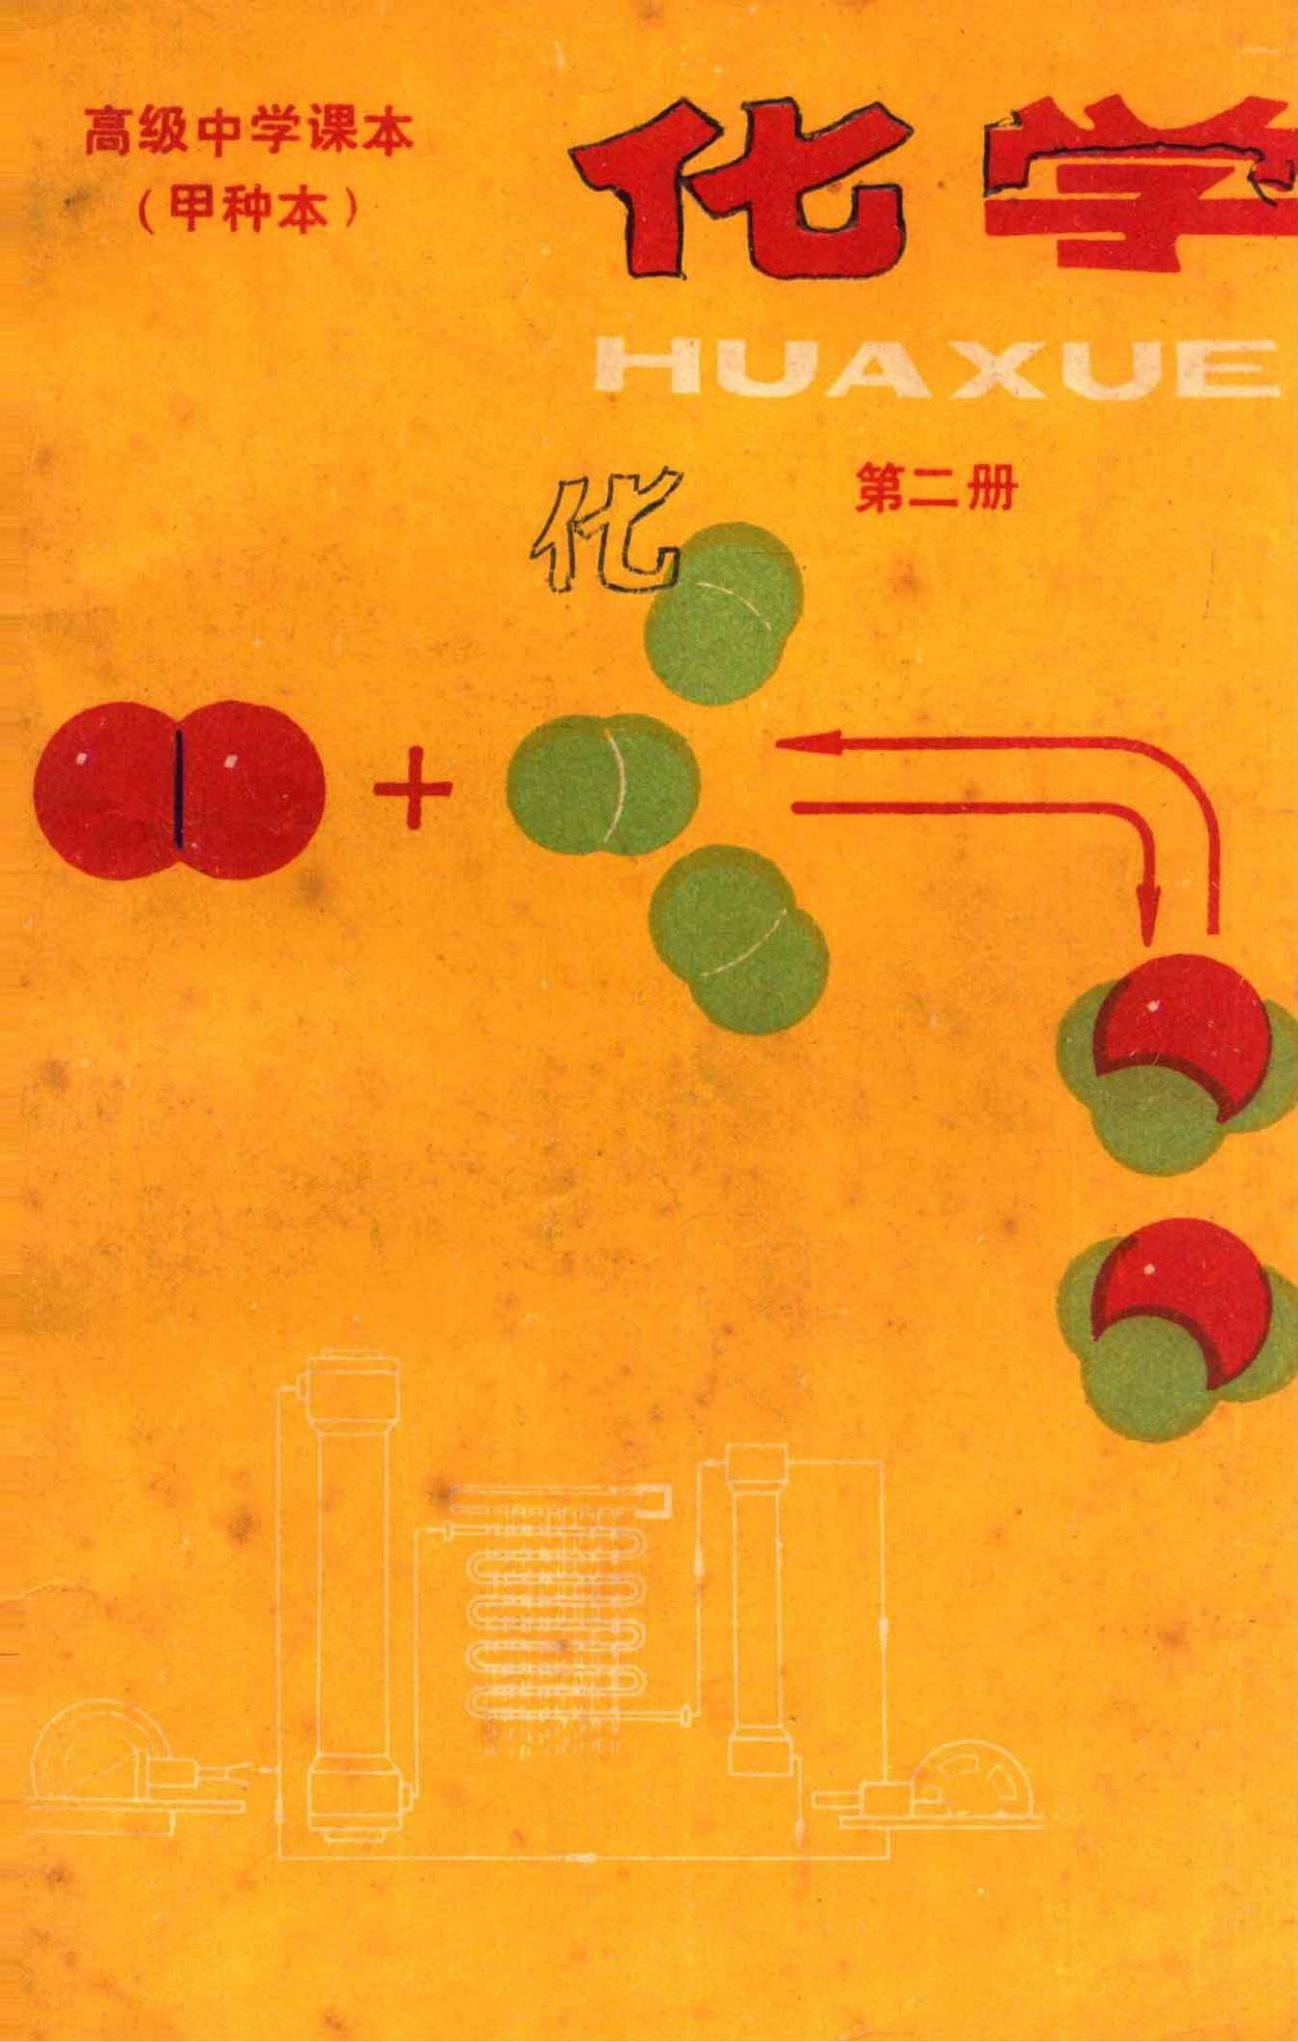
\includegraphics[max width=1.0\textwidth]{images/01912d13-9986-7822-a012-3f3f7be99dcb_1_875799.jpg}
\end{center}

\section*{说 明}

本书是根据教育部 1983 年 11 月颁发的高中化学教学纲要 (草案) 中的较高要求内容部分, 在人民教育出版社化学室编的六年制重点中学高中课本(试用本)《化学》第二册的基础上编写修改而成的。

教育部《关于颁发高中数学、物理、化学三科两种要求的教学纲要的通知》规定, 首批办好的重点中学, 可按较高要求的教学纲要进行教学, 其它三年制高中, 可根据学校的实际情况自行确定。因此, 本书可供三年制高中二年级选用。

参加本书编写和修改工作的有程名荣、张颂培、李文鼎等。北京师范大学化学系何少华也参加了编写修改工作。责任编辑是程名荣, 审定者是武永兴、梁英豪。

希望广大教师和研究中学化学教学的同志提出批评和修改意见。

\section*{目 录}

第一章 化学键和分子结构 -1

第一节 离子键 .1

第二节 共价键 - 6

第三节 非极性分子和极性分子 15

第四节 分子间作用力 \(\cdot {20}\)

第五节 氢键 .22

内容提要 .26

第二章 氮族 .29

第一节 氮族元素 .29

第二节 氮气. .32

第三节 氨 铵盐 .35

第四节 硝酸的工业制法. .43

第五节 硝酸 硝酸盐. 45

第六节 氧化-还原反应方程式的配平 .49

第七节 磷 磷酸 磷酸盐. -52

内容提要 .56

第三章 化学反应速度和化学平衡 .60

第一节 化学反应速度 .60

第二节 化学平 衡. .70

第三节 影响化学平衡的条件 -81

第四节 合成氨工业 .86

内容提要 .93

第四章 硅 胶体 .98

第一节 碳族元素 .98

第二节 硅及其重要的化合物 100

第三节 硅酸盐工业简述 107

第四节 股体 .110

内容提要 118

第五章 电解质溶液 122

第一节 强电解质和弱电解质 .122

第二节 电离度和电离常数 .126

第三节 水的电离和溶液的 \(\mathrm{{pH}}\) 值 .132

第四节 盐类的水 解 -137

第五节 酸碱的当量浓度 .143

第六节 酸和碱的中和反应 151

第七节 原电池 金属的腐蚀和防护 .154

第八节 电解和电镀 161

内容提要 169

第六章 镁 铝 176

第一节 金属键 176

第二节 镁和铝的性质 179

第三节 镁和铝的重要化合物 铝的冶炼 186

第四节 硬水及其软化 193

内容提要 193

学生实验 206

实验一 氨的制备和性质 铵离子的检验 .206

实验二 硝酸和硝酸盐的性质 .208

实验三 化学反应速度 化学平衡. .210

实验四 实验习题 .212

实验五 胶体的性质 .213

实验六 电解质溶液 .214

实验七 中和滴定 .216

实验八 中和热的测定 .218

实验九 原电池 金属的电化腐蚀 .220

实验十 电解 电镀. .222

实验十一 铝和氢氧化铝的化学性 质. .223

实验十二 分子量的测 定. 2.225

实验十三 实验习题. .227

\section*{第一章 化学键和分子结构}

我们已经学习了原子结构以及原子结构与元素性质递变关系的初步知识, 从本章起, 我们将学习有关原子怎样互相结合, 以及分子结构与物质性质的关系等初步知识。

\section*{第一节 离子键}

\section*{一、什么是化学键}

人们已经发现和合成了几百万种物质。为什么仅仅一百零几种元素的原子能够形成这么多种形形色色的物质呢? 原子是怎样互相结合的? 为什么两个氢原子能自动结合成氢分子, 而两个氦原子不能结合在一起? 为什么原子间按一定数目比互相结合? 原子结合成分子后, 性质为什么与原来的差别很大? 为了弄清以上的许多问题, 首先, 就要在原子结构知识基础上, 进一步研究原子在形成分子时的相互作用。

原子既然可以结合成分子, 原子之间必然存在着相互作用, 这种相互作用不仅存在于直接相邻的原子之间, 而且也存在于分子内的非直接相邻的原子之间。前一种相互作用比较强烈, 是使原子相互作用而联结成分子的主要因素, 破坏它要消耗比较大的能量。这种相邻的两个或多个原子之间强烈的相互作用, 通常叫做化学键。

化学键的主要类型有离子键、共价键、金属键等, 在这一章里, 我们先学习离子键和共价键。

\section*{二、离子键}

我们已经知道, 金属钠跟氯气能发生反应, 生成氯化钠:

\[
2\mathrm{{Na}} + {\mathrm{{Cl}}}_{2} = 2\mathrm{{NaCl}}
\]

因为钠原子的电离能很小, 容易失去电子, 而氯原子很容易结合电子。当钠跟氯气起反应时,钠原子的 \({3s}\) 电子转移到氯原子的 \({3p}\) 轨道上:

\begin{center}
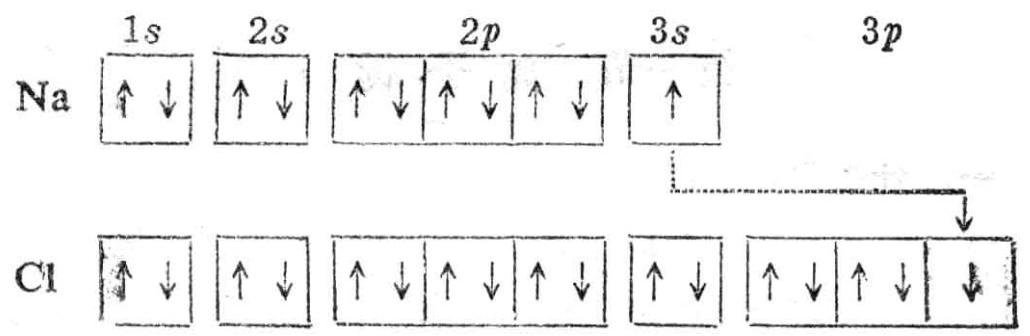
\includegraphics[max width=1.0\textwidth]{images/01912d13-9986-7822-a012-3f3f7be99dcb_7_558894.jpg}
\end{center}

钠原子失去 1 个 \({3s}\) 电子,形成类似氖原子的稳定电子层结构,带上一个单位正电荷,成为钠离子 \(\left( {\mathrm{{Na}}}^{ + }\right)\) ; 氯原子得到 1 个电子, 形成类似氩原子的稳定电子层结构, 带上一个单位负电荷, 成为氯离子(Cl-)。

\begin{center}
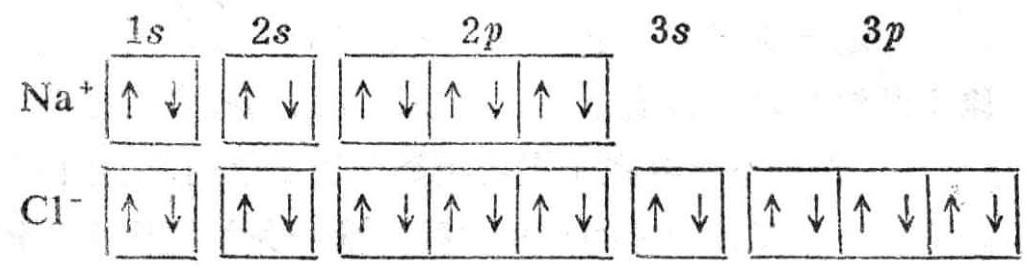
\includegraphics[max width=1.0\textwidth]{images/01912d13-9986-7822-a012-3f3f7be99dcb_7_866768.jpg}
\end{center}

钠离子和氯离子之间除了有静电相互吸引作用外, 还有电子与电子、原子核与原子核之间的相互排斥作用。当两种离子接近到某一定距离时, 吸引和排斥作用达到了平衡, 于是阴、阳离子之间就形成了稳定的化学键。

氯化钠的生成也可以用电子式来表示:

\[
{\mathrm{{Na}}}^{ \times } + \cdot \ddot{\mathrm{{Cl}}} : \rightarrow {\mathrm{{Na}}}^{ + }\left\lbrack {\dot{\mathrm{C}}\ddot{\mathrm{C}}1 : }\right\rbrack
\]

象氯化钠那样, 阴、阳离子间通过静电作用所形成的化学键叫做离子键。

活泼金属(如钾、钠、钙等)跟活泼非金属(如氯、溴等)化合时, 都能形成离子键。例如, 溴化钙就是由离子键所形成的。

\[
{\mathrm{{Ca}}}_{ \times }^{ \times } + 2 \cdot \ddot{\mathrm{{Br}}} : \rightarrow \left\lbrack { : \ddot{\mathrm{{Br}}}\dot{ \times }}\right\rbrack {\mathrm{{Ca}}}^{2 + }\left\lbrack {\dot{ \times }\ddot{\mathrm{{Br}}} : }\right\rbrack
\]

\section*{三、离子的结构特征}

\section*{1. 离子的电荷}

离子是带电荷的原子或原子团, 离子所带电荷的符号和数目与原子成键时得失电子数有关。例如, 镁跟氯起反应生成氯化镁,每个镁原子失去 2 个电子形成 \({\mathrm{{Mg}}}^{2 + }\) ,每个氯原子得到 1 个电子形成 \({\mathrm{{Cl}}}^{ - }\) 。

\section*{2. 离子的电子层结构}

主族元素所形成的离子的电子层一般是饱和的, 例如, \({\mathrm{{Li}}}^{ + }\text{、}{\mathrm{{Be}}}^{2 + }\) 等离子最外层是两个电子, \({\mathrm{{Na}}}^{ + }\text{、}{\mathrm{K}}^{ + }\text{、}{\mathrm{{Ca}}}^{2 + }\text{、}{\mathrm{{Mg}}}^{2 + }\) 、 \({\mathrm{{Al}}}^{3 + }\text{、}{\mathrm{O}}^{2 - }\text{、}{\mathrm{S}}^{2 - }\text{、}{\mathrm{F}}^{ - }\text{、}{\mathrm{{Cl}}}^{ - }\) 等离子最外层是 8 个电子; 副族和第 VIII 族元素所形成的离子的电子层常常是不饱和的, 例如, \({\mathrm{{Fe}}}^{3 + }\) 最外层有 13 个电子, \({\mathrm{{Co}}}^{3 + }\) 最外层有 14 个电子,等等。

\section*{3. 离子的半径}

由于阳离子是由原子失去外层电子而形成的, 所以, 阳离子的半径比相应的原子半径小, 例如:

\begin{center}
\adjustbox{max width=\textwidth}{
\begin{tabular}{|c|c|c|c|c|c|}
\hline
\phantom{X} & Li & \(\mathrm{{Na}}\) & \(\mathrm{K}\) & Rb & Cs \\
\hline
原子半径 \(\left( {10}^{-{10}}\right.\) 米 \()\) & 1.52 & 1.86 & 2.27 & 2.48 & 2.65 \\
\hline
离子半径 \(\left( {10}^{-{10}}\right.\) 米 \()\) & 0.68 & 0.97 & 1.33 & 1.47 & 1.67 \\
\hline
\end{tabular}
}
\end{center}

由于阴离子的外层电子数比相应的原子增多, 而核电荷没有变化, 所以, 阴离子的半径比相应的原子半径大。例如:

\begin{center}
\adjustbox{max width=\textwidth}{
\begin{tabular}{|c|c|c|c|c|}
\hline
\phantom{X} & F & Cl & \(\mathrm{{Br}}\) & I \\
\hline
原子半径 \(\left( {10}^{-{10}}\right.\) 米 & 0.71 & 0.99 & 1.14 & 1.33 \\
\hline
离子半径 \(\left( {10}^{-{10}}\right.\) 米 \()\) & 1.33 & 1.81 & 1.96 & 2.20 \\
\hline
\end{tabular}
}
\end{center}

对于电子层结构相同的离子,如 \({\mathrm{F}}^{ - }\text{、}{\mathrm{{Na}}}^{ + }\text{、}{\mathrm{{Mg}}}^{2 + }\text{、}{\mathrm{{Al}}}^{3 + }\) (它们的电子层结构与氖原子相同), 随着核电荷的逐渐增加, 离子半径逐渐减小。下面列出这几种离子的半径 \(\left( {10}^{-{10}}\right.\) 米)。

\begin{center}
\adjustbox{max width=\textwidth}{
\begin{tabular}{|c|c|c|c|}
\hline
\({\mathrm{F}}^{ - }\) & \({\mathrm{{Na}}}^{ + }\) & \({\mathrm{{Mg}}}^{2 + }\) & A1 3 + \\
\hline
1.33 & 0.97 & 0.65 & 0.50 \\
\hline
\end{tabular}
}
\end{center}

\section*{四、离子晶体}

以离子键结合的化合物就是离子化合物。离子化合物在室温下是以晶体形式存在。离子间通过离子键结合而成的品体叫做离子晶体。

在离子晶体中, 阴、阳离子按一定规律在空间排列。图 1-1 所示是 \(\mathrm{{NaCl}}\) 的晶体 结构,图 1-2 所示是 \(\mathrm{{CsCl}}\) 的晶体结构。

在 \(\mathrm{{NaCl}}\) 晶体中,每个 \({\mathrm{{Na}}}^{ + }\) 离子同时吸引着 6 个 \({\mathrm{{Cl}}}^{ - }\) 离子,每个 \({\mathrm{{Cl}}}^{ - }\) 离子也同时吸引着 6 个 \({\mathrm{{Na}}}^{ + }\) 离子。在 \({\mathrm{{CsCl}}}_{\mathrm{{fin}}}\) 体中,每个 \({\mathrm{{Cs}}}^{ + }\) 离子同时吸引着 8 个 \({\mathrm{{Cl}}}^{ - }\) 离子,每个 \({\mathrm{{Cl}}}^{ - }\) 离子也同时吸引着 8 个 \({\mathrm{{Cs}}}^{ + }\) 离子。因此,在 \(\mathrm{{NaCl}}\) 或 \(\mathrm{{CsCl}}\) 晶体中都不存在着单个的 \(\mathrm{{NaCl}}\) 分子或单个的 \(\mathrm{{CsCl}}\) 分子。但是, 在这两种晶体里, 阴、阳离子数目的比都是 \(1 : 1\) 。所以,严格地说, \(\mathrm{{NaCl}}\) 和 \(\mathrm{{CsCl}}\) 都是表示离子晶体中离子的个数比,它们都是用元素符号表示物质组成的化学式, 而不是表示分子组成的分子式。

\begin{center}
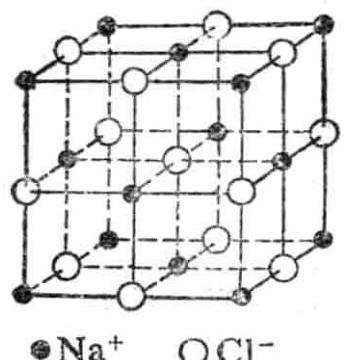
\includegraphics[max width=0.4\textwidth]{images/01912d13-9986-7822-a012-3f3f7be99dcb_10_571460.jpg}
\end{center}

\begin{center}
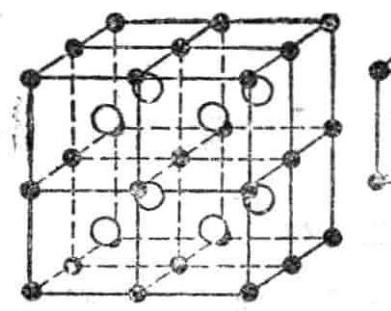
\includegraphics[max width=0.4\textwidth]{images/01912d13-9986-7822-a012-3f3f7be99dcb_10_385357.jpg}
\end{center}

\(\Delta {\mathrm{{Cs}}}^{ + }\) OCl-

图 1-1 NaCl 的晶体结构 图 1-2 CsCl 的晶体结构

在离子化合物中, 离子间存在着较强的离子键, 因此, 离子化合物一般说来, 硬度较高, 密度较大, 难于压缩, 难于挥发, 有较高的熔点和沸点。

\section*{习 题}

1. 用轨道表示式画出 \(\mathrm{{Mg}}\) 和 \(\mathrm{F}\) 原子的电子层和亚层的结构,并用电子式来表示 \({\mathrm{{MgF}}}_{2}\) 离子键的形成过程。

\({2f}\) 用轨道表示式画出 \(\mathrm{{Na}}\) 和 \(\mathrm{S}\) 原子的电子层和亚层的结构,并用电子式来表示 \({\mathrm{{Na}}}_{2}\mathrm{\;S}\) 离子键的形成过程。

3 用轨道表示式画出 \({\mathrm{{Ba}}}^{2 + }\text{、}{\mathrm{{Ag}}}^{ + }\text{、}{\mathrm{{Al}}}^{3 + }\text{、}{\mathrm{{Fe}}}^{2 + }\text{、}{\mathrm{{Fe}}}^{3 + }\) 的离子的电子层和亚层的结构。

4. 为什么说离子晶体中不存在单个的分子?

\section*{第二节 共 价 键}

\section*{一、共价键}

共价键是一种重要类型的化学键。现在举几种单质和化合物为例来说明共价键的形成和性质。

首先, 我们来学习氢原子是怎样结合成氢分子的。在通常状况下, 当一个氢原子和另一个氢原子接近时, 就相互作用而生成氢分子。

\[
\mathrm{H} + \mathrm{H} = {\mathrm{H}}_{2}
\]

在形成氢分子过程中, 电子不是从一个氢原子转移到另一个氢原子, 而是在两个氢原子间共用。这两个共用的电子, 填充了两个氢原子的 \({1s}\) 轨道,在两个原子核周围运动。这样,每个氢原子的 \({1s}\) 轨道是充满的,每个氢原子具有氦原子的稳定结构。

氢分子中的共用电子对可用下式表示:

\begin{center}
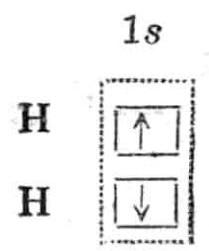
\includegraphics[max width=0.2\textwidth]{images/01912d13-9986-7822-a012-3f3f7be99dcb_11_655797.jpg}
\end{center}

氢分子的电子式为: \({\mathrm{H}}_{ \times }{\mathrm{H}}_{0}\)

在化学上常用一根短线表示一对共用电子, 因此, 氢分子又可表示为: \(\mathrm{H} - \mathrm{H}\) 。

从氢分子的电子云分布来看, 当两个电子自旋方向相同的氢原子互相接近时, 两个核间的电子云是稀疏的, 不能形成稳定的氢分子; 当两个电子自旋方向相反的氢原子互相接近时, 两个核间的电子云密集, 对两核产生引力, 能形成稳定的 \({\mathrm{H}}_{2}\) 分子(图 1-3)。

\begin{center}
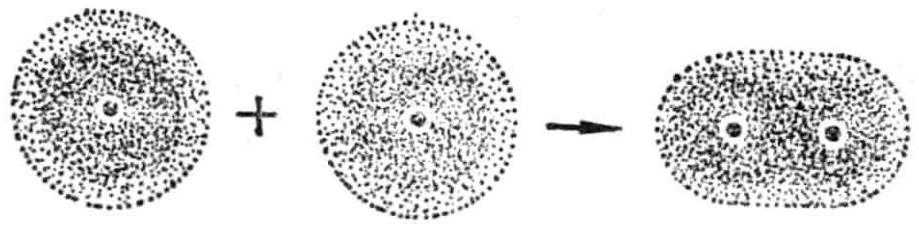
\includegraphics[max width=1.0\textwidth]{images/01912d13-9986-7822-a012-3f3f7be99dcb_12_238619.jpg}
\end{center}

图 1-3 氢分子的形成

氢分子的形成过程也可以用电子云的重叠来说明, 两个原子的电子云部分重叠以后, 两核间的电子云密集, 形成稳定分子。电子云重叠愈多, 分子愈稳定。

象氢分子那样, 原子间通过共用电子对 (电子云重叠) 所形成的化学键, 叫做共价键。

在分子中, 两个成键的原子的核间的平均距离叫做键长。例如, \(A\mathrm{H} - \mathrm{H}\) 键长 \({0.74} \times {10}^{-{10}}\) 米 (图 1-4), \(\mathrm{C} - \mathrm{C}\) 键长 \({1.54} \times {10}^{-{10}}\) 米, \(\mathrm{{Cl}} - \mathrm{{Cl}}\) 键长 \({1.98} \times {10}^{-{10}}\) 米。 一般说来, 两个原子之间所形成的键越短的, 键就越强, 越牢固。

\begin{center}
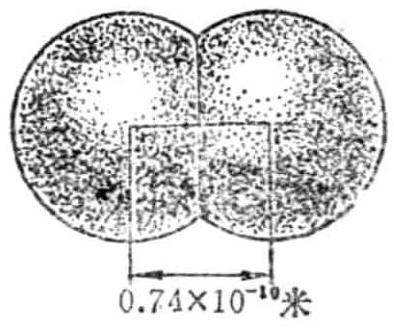
\includegraphics[max width=0.4\textwidth]{images/01912d13-9986-7822-a012-3f3f7be99dcb_12_265981.jpg}
\end{center}

图 1-4 \(\mathrm{H} - \mathrm{H}\) 键的键长

在 \(\mathrm{H}\) 原子形成 \({\mathrm{H}}_{2}\) 的过程中,要放出热量:

\[
\mathrm{H} + \mathrm{H} \rightarrow {\mathrm{H}}_{2} + {104.2}\text{千卡}
\]

由上式可知,1 摩尔 \(\mathrm{H}\) 原子和 1 摩尔 \(\mathrm{H}\) 原子作用,生成 1 摩尔 \({\mathrm{H}}_{2}\) 分子,放出 104.2 千卡热。上式也可说明 \({\mathrm{H}}_{2}\) 分子比 \(\mathrm{H}\) 原子的能量降低, \({\mathrm{H}}_{2}\) 分子比 \(\mathrm{H}\) 原子稳定。

如果要使 1 摩尔的 \({\mathrm{H}}_{2}\) 分子分裂为 2 摩尔 \(\mathrm{H}\) 原子,同样也需要吸收 104.2 千卡的热:

\[
{\mathrm{H}}_{2} + {104.2}\text{ 千卡 } \rightarrow \mathrm{H} + \mathrm{H}
\]

由上式可知,要拆开 1 摩尔的 \(\mathrm{H} - \mathrm{H}\) 键,需要吸收 104.2 千卡的能量,这个能量就是 \(\mathrm{H} - \mathrm{H}\) 键的键能。键能越大,表示化学键越牢固, 含有该键的分子越稳定。

表 1-1 列出了某些共价键的键能的数值。

表 1-1 某些共价键的键能 (千卡/摩尔)

\begin{center}
\adjustbox{max width=\textwidth}{
\begin{tabular}{|c|c|c|c|}
\hline
键 & 键 能 & 键 & 键 能 \\
\hline
\(\mathrm{H} - \mathrm{H}\) & 104.2 & \(\mathrm{C} - \mathrm{H}\) & 98.8 \\
\hline
C1-C1 & 58.0 & O—H & 110.6 \\
\hline
\(\mathrm{{Br}} - \mathrm{{Br}}\) & 46.3 & \(\mathrm{N} - \mathrm{H}\) & 93.4 \\
\hline
I-1 & 36.5 & \(\mathrm{H} - \mathrm{{Cl}}\) & 103.2 \\
\hline
\(\mathrm{C} - \mathrm{C}\) & 83.1 & \(\mathrm{H} - 1\) & 71.4 \\
\hline
\end{tabular}
}
\end{center}

\section*{[讨论] 现有反应}

\[
{\mathrm{H}}_{2} + {\mathrm{{Cl}}}_{2} = 2\mathrm{{HCl}} + {44.2}\text{ 千卡 }
\]

试讨论反应物 \(\left( {\mathrm{H} - \mathrm{H}\text{、}\mathrm{{Cl}} - \mathrm{{Cl}}}\right)\) 和生成物 \(\left( {\mathrm{H} - \mathrm{{Cl}}}\right)\) 的键能与这个反应的反应热的关系。

双原子的 \({\mathrm{{Cl}}}_{2}\) 分子的形成跟 \({\mathrm{H}}_{2}\) 分子相似。两个氯原子共用一对电子,这一对电子互相充填未充满的 \({3p}\) 轨道,这样, 每个氯原子具有氩原子的电子层结构。

\begin{center}
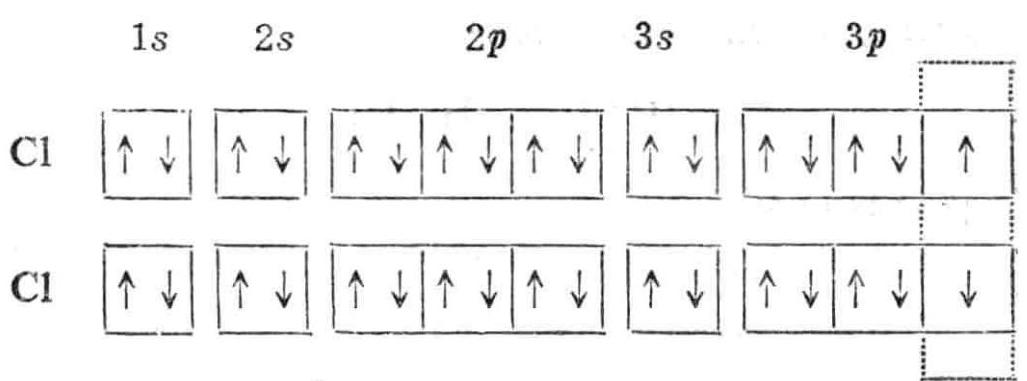
\includegraphics[max width=1.0\textwidth]{images/01912d13-9986-7822-a012-3f3f7be99dcb_14_931588.jpg}
\end{center}

氯分子可以用下列式子表示:

\[
{}_{\times \times }^{\times \times }{}_{\times \times }^{\times \times }{}_{\cdot \cdot }^{\cdot \cdot }{}_{\cdot \cdot }^{\cdot \cdot }\;\mathrm{{Cl}} - \mathrm{{Cl}}
\]

氮分子的形成跟氯分子相似,只是有三对 \(p\) 电子共用,形成三键。

\begin{center}
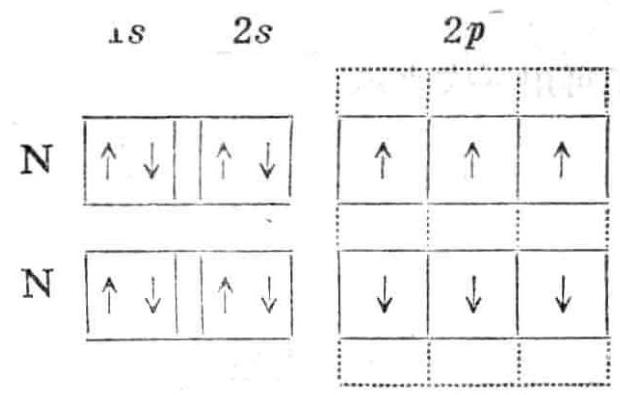
\includegraphics[max width=0.7\textwidth]{images/01912d13-9986-7822-a012-3f3f7be99dcb_14_219593.jpg}
\end{center}

氮分子可以用下列式子表示:

\[
{}_{ \times }^{ \times }{\mathrm{N}}_{ \times }^{ \times }\vdots \mathrm{N} : \;\mathrm{N} \equiv \mathrm{N}
\]

现在举两个不同原子以共价键结合成分子的例子, 如

\begin{center}
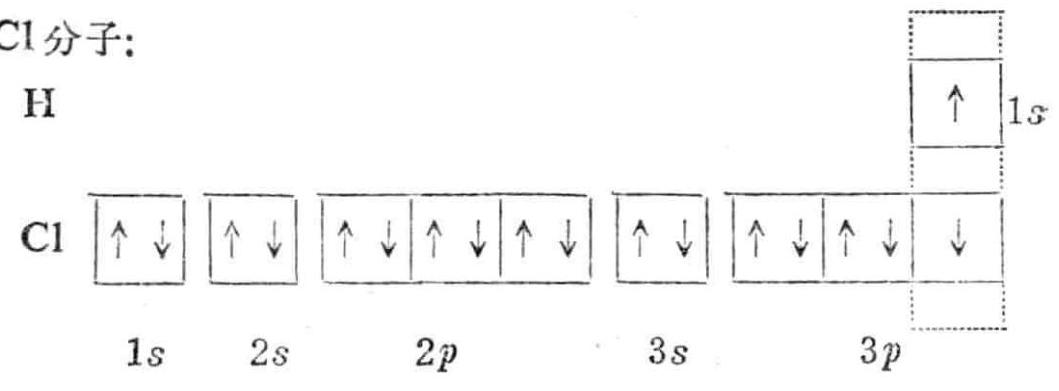
\includegraphics[max width=1.0\textwidth]{images/01912d13-9986-7822-a012-3f3f7be99dcb_14_721329.jpg}
\end{center}

\(\mathrm{{HCl}}\) 分子可用下列式子表示:

\[
{\mathrm{H}}_{ \times }\ddot{\mathrm{{Cl}}} : \;\mathrm{H} - \mathrm{{Cl}}
\]

再如 \({\mathrm{H}}_{2}\mathrm{O}\) 分子:

\begin{center}
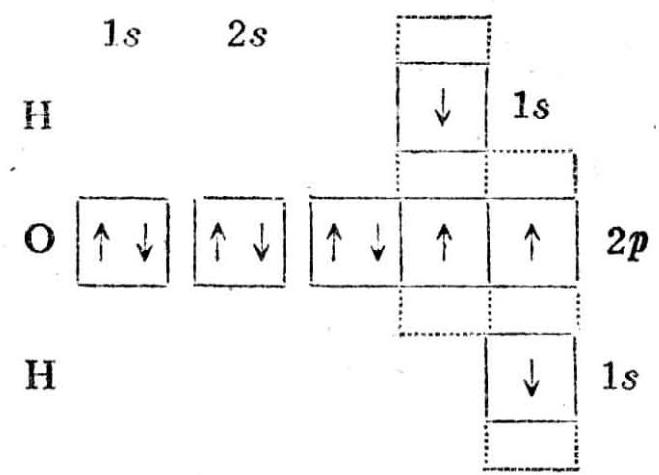
\includegraphics[max width=0.7\textwidth]{images/01912d13-9986-7822-a012-3f3f7be99dcb_15_743845.jpg}
\end{center}

\({\mathrm{H}}_{2}\mathrm{O}\) 分子可用下式表示:

\begin{center}
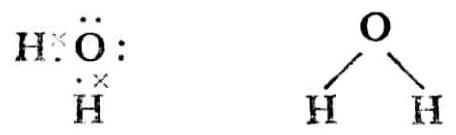
\includegraphics[max width=0.5\textwidth]{images/01912d13-9986-7822-a012-3f3f7be99dcb_15_422269.jpg}
\end{center}

\section*{二、共价键的饱和性和方向性}

根据上面学过的几种单质和化合物中共价键的形成的知识, 我们可以看出共价键具有以下两个共同的性质。

\section*{1. 饱和性}

由于一个原子的未成对电子跟另一个原子的自旋相反的电子配对成键后, 就不能跟第三个电子配对成键, 因此, 一个原子有几个未成对电子, 就可和几个自旋相反的电子配对成键。这就是共价键的饱和性。例如, 硫原子和氢原子能结合生成硫化氢分子,因为每个硫原子有两个未成对的 \({3p}\) 电子, 每个氢原子有一个未成对的 \({1s}\) 电子,所以,一个硫原子可以跟两个氢原子结合成 \({\mathrm{H}}_{2}\mathrm{\;S}\) 分子,而不可能生成 \({\mathrm{H}}_{3}\mathrm{\;S}\) 或 \({\mathrm{H}}_{4}\mathrm{\;S}\) 的分子。

\section*{2. 方向性}

我们知道,除 \(s\) 轨道的电子云是球形对称的以外,其它轨道 ( \(p\) 轨道、 \(d\) 轨道等) 的电子云都具有一定的伸展方向。在形成共价键时, 成键电子的电子云重叠愈多, 核间电子云密度愈大, 形成的共价键愈稳固。因此, 共价键的形成尽可能沿着电子云密度最大的方向。例如, 在硫原子跟氢原子结合生成 \({\mathrm{H}}_{2}\mathrm{\;S}\) 分子时, 因为硫原子的最外层两个不成对的 \({3p}\) 电子的电子云互成直角,氢

\begin{center}
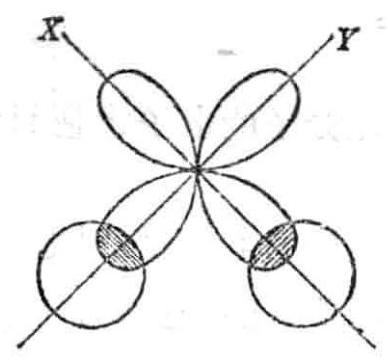
\includegraphics[max width=0.4\textwidth]{images/01912d13-9986-7822-a012-3f3f7be99dcb_16_224219.jpg}
\end{center}

原子的 \({1s}\) 电子云要沿着直角的 图 1-5 硫化氢分子的成键方向跟 \({3p}\) 电子云重叠,这样 \({\mathrm{H}}_{2}\mathrm{\;S}\) 分子中两个共价键的夹角应接近 \({90}^{ \circ }\) (图 1-5)。

在分子中键和键之间的夹角叫做键角。例如, 水分子中两个 \(\mathrm{O} - \mathrm{H}\) 键间的夹角是 \({104.5}^{ \circ }\) ,二氧化碳分子中两个 \(\mathrm{C} = \mathrm{O}\) 键成直线,夹角是 \({180}^{ \circ }\) ,氨分子中两个 \(\mathrm{N} - \mathrm{H}\) 键间的夹角是 \({107}^{ \circ }{18}^{\prime }\) ,甲烷分子中两个 \(\mathrm{C} - \mathrm{H}\) 键间的夹角是 \({109}^{ \circ }{28}^{\prime }\) 。

\section*{三、配位键}

上面介绍的共价键中, 电子对都是由两个原子各提供未成对电子而形成的。还有一类特殊的共价键, 电子对是由一个原子单方面提供而跟另一个原子共用的。这样的共价键叫做配位键。

现在以铵离子 \(\left( {\mathrm{{NH}}}_{4}^{ + }\right)\) 为例来说明配位键的形成。我们已经知道, 氨跟酸起反应生成铵盐, 例如:

\[
{\mathrm{{NH}}}_{3} + \mathrm{{HCl}} = {\mathrm{{NH}}}_{4}\mathrm{{Cl}}
\]

这个反应可用离子方程式来表示:

\[
{\mathrm{{NH}}}_{3} + {\mathrm{H}}^{ + } = {\mathrm{{NH}}}_{4}^{ + }
\]

上式表示氨跟能产生氢离子的物质(酸)相作用, 生成铵离子。

氨分子的电子式是 \(\mathrm{H} : \begin{matrix} \mathrm{H} \\ \mathrm{N} \\ \mathrm{H} \\ \mathrm{H} \end{matrix} :\) ,氮原子上有一对没有跟其它

原子共用的电子 (孤对电子)。氢离子 \(\left( {\mathrm{H}}^{ + }\right)\) 是氢原子失去 \({1s}\) 电子而形成的,它具有一个 \({1s}\) 空轨道。当氨分子跟氢离子相作用时, 氨分子上的孤对电子进入氢离子的空轨道, 这一对电子在氮、氢原子间共用,形成了配位键。配位键可以用 \(\mathrm{A} \rightarrow \mathrm{B}\) 来表示, 其中 A 是提供孤对电子的原子, B 是具有空轨道接受电子的原子。

\begin{center}
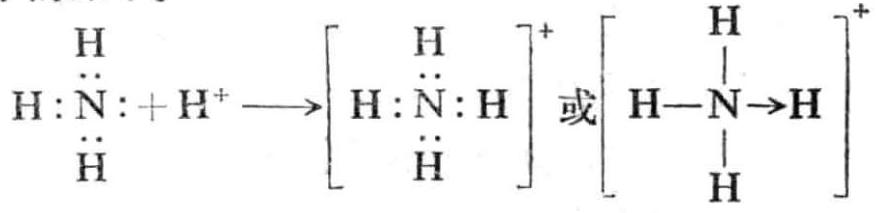
\includegraphics[max width=1.0\textwidth]{images/01912d13-9986-7822-a012-3f3f7be99dcb_17_176417.jpg}
\end{center}

在铵离子中,虽然有一个 \(\mathrm{N} - \mathrm{H}\) 键跟其他三个 \(\mathrm{N} - \mathrm{H}\) 键的形成过程不同, 但是它们的键长、键能、键角都是一样的, 四个键表现的化学性质也完全相同。所以, 铵离子通常就用下式表示:

\begin{center}
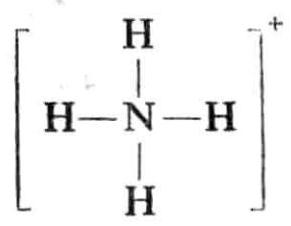
\includegraphics[max width=0.3\textwidth]{images/01912d13-9986-7822-a012-3f3f7be99dcb_17_186848.jpg}
\end{center}

\section*{四、原子晶体}

我们已经知道, 金刚石和石墨都是由碳原子形成的单质, 但它们的性质很不相同。这是由于它们的晶体结构不相同的缘故。

\begin{center}
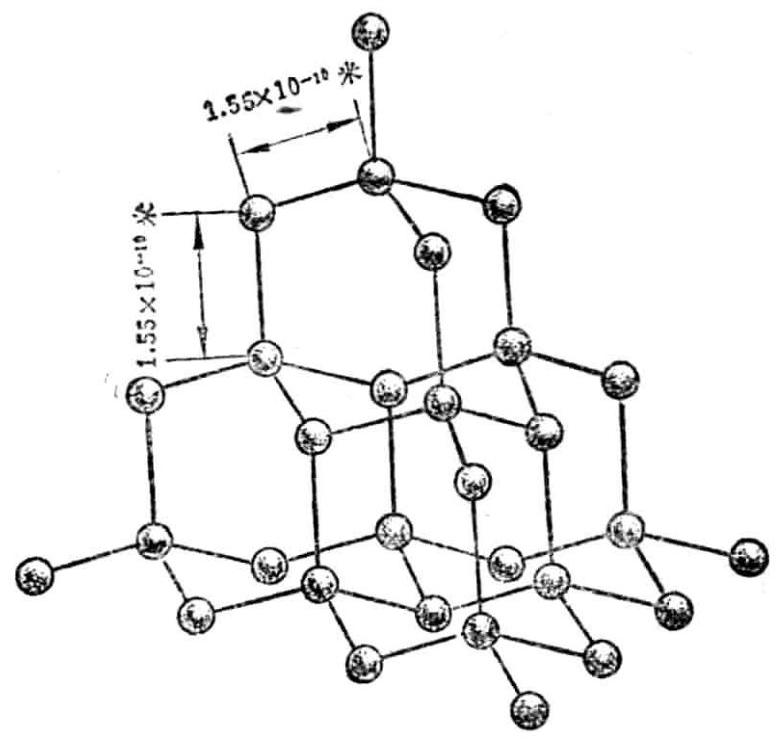
\includegraphics[max width=0.8\textwidth]{images/01912d13-9986-7822-a012-3f3f7be99dcb_18_466715.jpg}
\end{center}

图 1-6 金刚石的晶体结构示意图

在金刚石的晶体里, 每个碳原子都被相邻的 4 个碳原子包围, 处于 4 个碳原子的中心, 以共价键跟这 4 个碳原子结合, 成为正四面体结构, 这些正四面体结构向空间发展, 构成一种坚实的、彼此联结的空间网状晶体 (图 1-6)。相邻的碳原子间共用一对电子,共价键的键长为 \({1.55} \times {10}^{-{10}}\) 米,键角为 \({109}^{ \circ }{28}^{\prime }\) 。这种相邻原子间以共价键相结合而形成空间网状结构的晶体, 叫做原子晶体。

石墨的晶体 (图 1-7) 是层次结构, 在每一层内, 碳原子排成六边形, 一个个六边形排列成平面的网状结构 (图 1-8), 每

\begin{center}
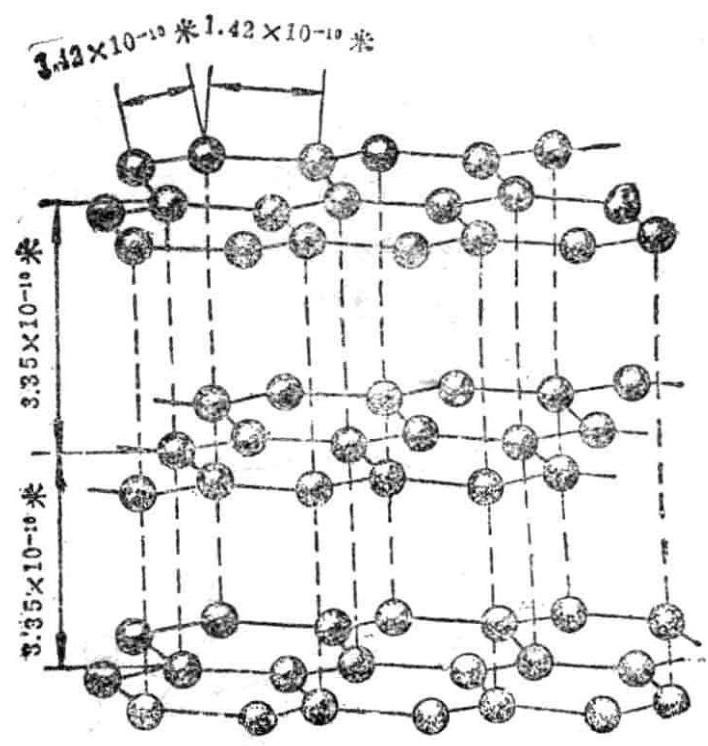
\includegraphics[max width=0.8\textwidth]{images/01912d13-9986-7822-a012-3f3f7be99dcb_19_268531.jpg}
\end{center}

图 1-7 石墨的晶体结构示意图

一个碳原子都跟其他 3 个碳原子相结合。在同一层内, 相邻的碳原子以共价键结合, 键长为 \({1.42} \times {10}^{-{10}}\) 米。相邻的两层间的距离为 \({3.35} \times {10}^{-{10}}\) 米。在石墨的每个碳原子最外电子层的 4 个电子中, 有 3 个电子形成单键。第四个电子形成比较复杂的键,可以在层内移动 \({}^{\left( 1\right) }\) 。

\begin{center}
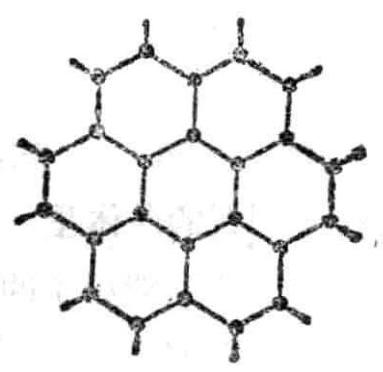
\includegraphics[max width=0.4\textwidth]{images/01912d13-9986-7822-a012-3f3f7be99dcb_19_995840.jpg}
\end{center}

图 1-8 石墨的晶体结构俯视图

在原子晶体中, 原子间用

较强的共价键相结合, 因而熔点和沸点较高, 如金刚石的熔点高于 \({3550}^{ \circ }\mathrm{C}\) ,沸点为 \({4827}^{ \circ }\mathrm{C}\) ,石墨的熔点为 \({3652} - {3697}^{ \circ }\mathrm{C}\) (升华),沸点为 \({4827}^{ \circ }\mathrm{C}\) ,它们都难溶于溶剂。

\customfootnote{

① 严格地说, 石墨是一种过渡型晶体。

}

\section*{习 题}

1. 用轨道表示式画出 \(\mathrm{F}\) 原子和 \(\mathrm{{Br}}\) 原子的电子层和亚层的结构,并表示 \({\mathrm{F}}_{2}\) 分子、 \({\mathrm{{Br}}}_{2}\) 分子的形成过程。

2. 用轨道表示式画出 \(\mathbf{N}\) 原子和 \(\mathbf{H}\) 原子的电子层和亚层的结构,并表示 \({\mathrm{{NH}}}_{3}\) 分子的形成过程。

3. 什么是共价键的饱和性和方向性?

4. 惰性气体为什么不能形成双原子分子?

5. 从 \({\mathrm{H}}_{2}\text{、}{\mathrm{{Cl}}}_{2}\text{、}{\mathrm{{Br}}}_{2}\text{、}{\mathrm{I}}_{2}\) 的键能来看,哪种分子最稳定,哪种最不稳定?

6. 在酸的水溶液中, \({\mathrm{H}}^{ + }\) 离子常与 \({\mathrm{H}}_{2}\mathrm{O}\) 分子结合成 \({\mathrm{H}}_{3}{\mathrm{O}}^{ + }\) 离子,试从配位键来解释 \({\mathrm{H}}_{3}{\mathrm{O}}^{ + }\) 的形成。

\section*{第三节 非极性分子和极性分子}

\section*{一、非极性键和极性键}

在单质分子中, 同种原子形成共价键, 两个原子吸引电子的能力相同, 共用电子对不偏向任何一个原子, 这两个电子在键的中央出现的机会最多, 成键的原子都不显电性。这样的共价键叫做非极性共价键, 简称非极性键。例如, H-H 键, \(\mathrm{{Cl}} - \mathrm{{Cl}}\) 键都是非极性键。

在化合物分子中, 不同种原子形成共价键, 由于不同原子吸引电子的能力不同, 共用电子对必然偏向吸引电子能力强的原子一方, 也就是说, 靠近吸引电子能力强的原子一方电子云比较密集。因而吸引电子能力较强的原子就带部分负电荷, 吸引电子能力较弱的原子就带部分正电荷。这样的共价键叫做极性共价键, 简称极性键。例如, 在 HCl 分子里, C1 原子吸引电子的能力比 \(\mathrm{H}\) 原子强,成键的电子云偏向 \(\mathrm{{Cl}}\) 原子一边,使 \(\mathrm{{Cl}}\) 原子带部分负电荷, \(\mathrm{H}\) 原子带部分正电荷。因此, \(\mathrm{{HCl}}\) 分子可以用如下的电子式来表示:

\[
\mathrm{H}\dot{\dot{ * }}\ddot{\mathrm{C}}\text{1:}
\]

\section*{二、电负性}

分子中两个成键原子吸引电子能力的大小是用元素的电负性来表示的。电负性数值的大小在 \({0.7} - 4\) 之间。电负性数值越大, 成键原子吸引电子的能力越大。表 1-2 所列是常见元素的电负性数值。

表 1-2 常见元素的电负性

\begin{center}
\adjustbox{max width=\textwidth}{
\begin{tabular}{|c|c|c|c|c|c|c|c|}
\hline
元素 符号 & 电负性 & 元素 符号 & 电负性 & 元素 符号 & 电负性 & 元素 符号 & 电负性 \\
\hline
\(\mathrm{H}\) & 2. 1 & Ba & 0.9 & Pb & 1.9 & F & 4.0 \\
\hline
Li & 1.0 & B & 2.0 & N & 3.0 & C1 & 3. 0 \\
\hline
\(\mathrm{{Na}}\) & 0.9 & A1 & 1. 5 & P & 2. 1 & \(\mathrm{{Br}}\) & 2.8 \\
\hline
\(\mathrm{K}\) & 0.8 & Ga & 1.6 & As & 2.0 & 1 & 2. 5 \\
\hline
Rb & 0.8 & In & 1.7 & Sb & 1.9 & \(\mathrm{{Cu}}\) & 1.9 \\
\hline
Cs & 0.7 & T1 & 1.8 & \(\mathrm{{Bi}}\) & 1.9 & Ag & 1.9 \\
\hline
Be & 1.5 & C & 2.5 & O & 3. 5 & Au & 2. 4 \\
\hline
\(\mathrm{{Mg}}\) & 1.2 & Si & 1. 8 & S & 2. 5 & Zn & 1. 6 \\
\hline
\(\mathrm{{Ca}}\) & 1.0 & Ge & 1.8 & Se & 2. 4 & \(\mathrm{{Cd}}\) & 1.7 \\
\hline
\(\mathrm{{Sr}}\) & 1.0 & Sn & 1.8 & Te & 2.1 & \(\mathrm{{Hg}}\) & 1.9 \\
\hline
\end{tabular}
}
\end{center}

从表 1-2 可以看出, 金属的电负性较小, 金属的电负性越小, 它的活动性越大; 非金属的电负性较大, 非金属的电负性越大, 它的活动性越大。

根据两种元素的电负性数值, 可以大体上推测它们形成的键的类型和共价键极性的大小。

活泼的金属原子和活泼的非金属原子通过外层电子转移而形成离子键。活泼金属的电负性较小, 活泼非金属的电负性较大, 所以, 形成离子键的两种原子的电负性数值的差比较大。单质分子是由同种原子组成的, 原子的电负性数值的差等于零, 也就是说, 形成非极性键的原子间的电负性数值的差等于零。形成极性键的原子的电负性数值的差介于形成离子键的原子电负性数值的差和零之间。由此可知, 形成化学键的两个原子, 它们的电负性的数值的差越大, 形成的键的极性也越大。

\section*{三、非极性分子和极性分子}

如果分子中的键都是非极性的, 共用电子对不偏向任何一个原子, 整个分子的电荷分布是均匀的、对称的, 这样的分子叫做非极性分子。以非极性键结合而成的分子都是非极性分子,如 \({\mathrm{H}}_{2}\text{、}{\mathrm{O}}_{2}\text{、}{\mathrm{{Cl}}}_{2}\text{、}{\mathrm{\;N}}_{2}\) 等。

以极性键结合的双原子分子如 \(\mathrm{{HC}}1\) 分子里,共用电子对倾向氯原子, 氯原子一端带部分负电荷, 氢原子一端带部分正电荷, 整个分子的电荷分布是不均匀的、不对称的, 这样的分子叫做极性分子, 以极性键结合的双原子分子都是极性分子。

以极性键结合的多原子分子, 可能是极性分子, 也可能是非极性分子, 这决定于分子中各键的空间排列。

例如, 二氧化碳是直线型分子, 两个氧原子对称地位于碳原子的两侧。

\[
\mathrm{O} = \mathrm{C} = \mathrm{O}
\]

在 \({\mathrm{{CO}}}_{2}\) 分子中, \(\mathrm{C} = \mathrm{O}\) 键是极性键,因为氧的电负性大于碳,共用电子对偏向于氧原子,氧原子带部分负电荷。从 \({\mathrm{{CO}}}^{2}\) 分子总体来看,两个 \(\mathrm{C} = \mathrm{O}\) 键是对称排列的,两键的极性互相抵消, 整个分子没有极性。所以, 二氧化碳是非极性分子。

水的分子不是直线型的,两个 \(\mathrm{O} - \mathrm{H}\) 键之间的键角约为 \({104.5}^{ \circ }\) 。

\begin{center}
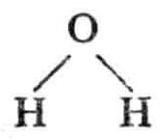
\includegraphics[max width=0.2\textwidth]{images/01912d13-9986-7822-a012-3f3f7be99dcb_23_841301.jpg}
\end{center}

\(\mathrm{O} - \mathrm{H}\) 键是极性键,氧原子的电负性大于氢原子,共用电子对偏向于氧原子, 氧原子带部分负电荷, 氢原子带部分正电荷。由于氢原子分布在分子的一端, 因而氢原子一端带正电荷, 氧原子一端带负电荷, 水分子是个极性分子。

三角锥形的氨分子 ( \(\mathrm{N} - \mathrm{H}\) 键间夹角是 \({107}^{ \circ }{18}^{\prime }\) ) 也是极性分子。

\begin{center}
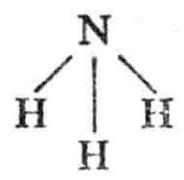
\includegraphics[max width=0.2\textwidth]{images/01912d13-9986-7822-a012-3f3f7be99dcb_23_457605.jpg}
\end{center}

四氯化碳分子中, 碳原子位于正四面体的中心, 4 个氯原

子位于正四面体的 4 个顶角 (C-C1 键夹角是 \({109}^{ \circ }{28}^{\prime }\) ),对称地排列于碳原子的周围, \({\mathrm{{CCl}}}_{4}\) 是非极性分子。

\begin{center}
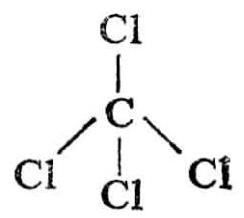
\includegraphics[max width=0.3\textwidth]{images/01912d13-9986-7822-a012-3f3f7be99dcb_24_696485.jpg}
\end{center}

[实验 1-1] 在酸式滴定管中注入 30 毫升蒸馏水, 夹在滴定管夹上, 滴定管下端放一大烧杯。打开活栓, 让水缓慢下流如线状。把摩擦带电的玻璃棒或塑料棒接近水流, 观察水流的方向有没有变化。

如用 \({\mathrm{{CCl}}}_{4}\) 代替水作上述实验,有什么现象发生?

[讨论] 根据人们的实践经验, 极性分子组成的溶质易溶于极性分子组成的溶剂, 非极性分子组成的溶质易溶于非极性分子组成的溶剂, 试解释下列现象:

(1)氯化氢易溶于水, 不易溶于汽油(非极性);

(2)碘易溶于 \({\mathrm{{CCl}}}_{4}\) ,不易溶于水;

(3)石蜡(非极性)易溶于汽油,不易溶于水。

你还能想出哪些在生活中接触到的有关物质的溶解性与极性的关系的例子。

\section*{习 题}

1. 什么是非极性键? 什么是极性键? 举例说明。

2. 根据电负性数值, 判断下列物质中的化学键类型:

(1) \(\mathrm{{KBr}},\left( 2\right) {\mathrm{{CCl}}}_{4},\left( 3\right) {\mathrm{N}}_{2},\left( 4\right) \mathrm{{CaO}},\left( 5\right) {\mathrm{H}}_{2}{\mathrm{\;S}}_{0}\)

3. 具有极性键的化合物是否一定是极性分子? 举例说明。

4. 下列分子中哪些是非极性分子? 哪些是极性分子?

(1) \(\mathrm{{NO}},\left( 2\right) {\mathrm{H}}_{2}\mathrm{\;S}\) ,(3) \({\mathrm{{CS}}}_{2}\) (直线型分子,两个 \(\mathrm{S}\) 原子在 C 原子两侧),(4) \({\mathrm{{SO}}}_{2}\) (键角为 \({120}^{ \circ }\) )。

\section*{第四节 分子间作用力}

\section*{一、分子间作用力}

氢气、氯气、二氧化碳等物质在常温时是气体, 在降低温度、增大压强时能够凝结为液体, 进一步能凝固为固体。气态物质能够转变为液态和固态, 也就是说, 气态物质分子能缩短彼此间的距离, 并由无规则运动转变为有规则排列, 这说明物质的分子间存在着作用力, 这种分子间的作用力又叫做范德华力 \(\text{①}\) 。

我们已经知道, 化学键是原子结合成分子时, 相邻原子间强烈的相互作用。通常化学键的键能为 30-200 千卡/摩尔。 而分子间力要比化学键弱得多, 通常约每摩尔几个千卡。例如, \(\mathrm{{HCl}}\) 分子的 \(\mathrm{H} - \mathrm{{Cl}}\) 键能为 103.2 千卡/摩尔,而 \(\mathrm{{HCl}}\) 分子间的作用力为 5.05 千卡/摩尔。

分子间作用力按其实质来说也是一种电性的吸引力。例如, 极性分子和极性分子之间以其带异性电荷的一端互相吸引。非极性分子的电荷分布虽然是均匀的, 但在某一瞬间, 由子核与电子云的相对运动, 会使分子产生瞬间的极性, 这样就会产生分子间的引力。①

\customfootnote{

① 范德华(J. D. van der Waals, 1837-1923), 荷兰物理学家。 他首先研究了分子间的作用力, 即以他的名字命名。

}

分子间作用力的大小对物质的熔点、沸点、溶解度等有影响。例如, 分子间作用力越大, 克服分子间引力使物质熔化和气化就需要更多的能量。

影响分子间作用力的因素很多, 例如, 组成和结构相似的物质随着分子量的增大, 分子间的作用力也增大, 表现在熔点和沸点的升高上 (见表 1-3、表 1-4)。

表 1-3 卤素单质的熔点和沸点

\begin{center}
\adjustbox{max width=\textwidth}{
\begin{tabular}{|c|c|c|c|}
\hline
卤素单质 & 熔点 \(\left( {{}^{ \circ }\mathrm{C}}\right)\) & \multicolumn{2}{|c|}{沸点 \(\left( {{}^{ \circ }\mathrm{C}}\right)\)} \\
\hline
\(\begin{array}{ll} \text{ 氟 }{\mathrm{F}}_{2} & \text{ 分 } \\ \text{ 氯 }{\mathrm{{Cl}}}_{2} & \text{ 子 } \\ \text{ 溴 }{\mathrm{{Br}}}_{2} & \text{ 盐 } \\ \text{ 溴 }{\mathrm{{Br}}}_{2} & \text{ 大 } \end{array}\) & \(- {101}\) \(- {219.6}\) \(- - {7.2}\) 熔点升高 & -188.1 \(- {34.6}\) 58.78 & 沸点升高 \\
\hline
\phantom{X} & 113.5 & 184.4 & \phantom{X} \\
\hline
\end{tabular}
}
\end{center}

表 1-4 四卤化碳的熔点和沸点

\begin{center}
\adjustbox{max width=\textwidth}{
\begin{tabular}{|c|c|c|c|c|}
\hline
四卤化碳 & \multicolumn{2}{|c|}{熔点 \(\left( {{}^{ \circ }\mathrm{C}}\right)\)} & \multicolumn{2}{|c|}{沸点 \(\left( {{}^{ \circ }\mathrm{C}}\right)\)} \\
\hline
\({\mathrm{{CF}}}_{4}\) \({\mathrm{{CCl}}}_{4}\) \({\mathrm{{CBr}}}_{4}\) \({\mathrm{{CI}}}_{4}\) 分子量增大 & \(- {184}\) \(- {22.9}\) 90.1 171 (分解) & 熔点升高 & \(- {128}\) 76.5 189.5 \(-\) & 沸点升高 \\
\hline
\end{tabular}
}
\end{center}

分子间作用力的大小除与分子量的大小有关外, 还与分子的极性、分子的形状等因素有关。

\customfootnote{

① 课文里的楷体字教材是供学生课外阅读的。以下同。

}

\section*{二、分子晶体}

\begin{center}
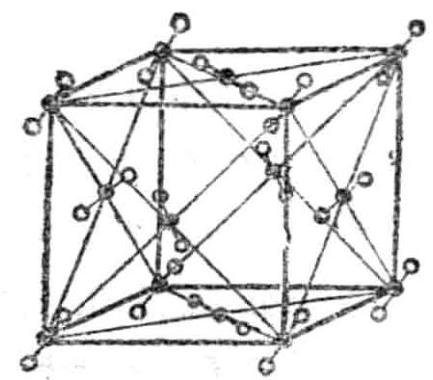
\includegraphics[max width=0.5\textwidth]{images/01912d13-9986-7822-a012-3f3f7be99dcb_27_304390.jpg}
\end{center}

60 代表 \({\mathrm{{CO}}}_{2}\) 一个分子

图 1-9 固态二氧化碳的晶体结构示意图

分子间以分子间作用力互相结合的晶体叫做分子晶体。非极性分子和极性分子都可以形成分子晶体。例如, 卤素、惰性气体、 氧、二氧化碳、氨、卤化氢等等都能形成分子晶体。图 1-9 所示是固态二氧化碳(干冰)的晶体结构示意图。

由于分子间作用力很弱, 因此, 分子晶体具有较低的熔点、沸点和较小的硬度。

\section*{习 题}

1. 为什么氯的熔点和沸点很低, 而氯化钠的熔点和沸点很高?

2. 为什么随着原子序数的增加, 惰性气体的熔点和沸点都逐渐升高?

3. 当干冰熔化和气化时, \({\mathrm{{CO}}}_{2}\) 分子内的 \(\mathrm{C} = \mathrm{O}\) 键有没有变化?

4. 已知 \({\mathrm{{BBr}}}_{3}\) 的熔点是 \(- {46}^{ \circ }\mathrm{C},\mathrm{{KBr}}\) 的熔点是 \({734}^{ \circ }\mathrm{C}\) ,试估计它们各属于哪一类晶体。

\section*{第五节 氢 键}

上节已介绍过某些相似物质的分子间作用力随着分子量的增大而增大, 以及它们的熔点和沸点也随着升高的事实。但是, 有些氢化物的熔点和沸点的递变与以上规律不完全符合。 让我们来看一下表 1-5 和图 1-10。

表 1-5 一些氢化物的沸点 \(\left( {{}^{ \circ }\mathrm{C}}\right)\)

\begin{center}
\adjustbox{max width=\textwidth}{
\begin{tabular}{|c|c|c|c|c|c|c|}
\hline
碳 族 & \phantom{X} & 氮 族 & \phantom{X} & 氧 族 & \multicolumn{2}{|c|}{卤族} \\
\hline
\({\mathrm{{CH}}}_{4}\) & \(- {160}\) & \({\mathrm{{NH}}}_{3}\) & \(- {33}\) & \({\mathrm{H}}_{2}\mathrm{O}\) 100 & HF & 20 \\
\hline
\({\mathrm{{SiH}}}_{4}\) & \(- {112}\) & \({\mathrm{{PH}}}_{3}\) & \(- {88}\) & \({\mathrm{H}}_{2}\mathrm{\;S}\) \(- {61}\) & HCl & \(- {85}\) \\
\hline
\({\mathrm{{GeH}}}_{4}\) & \(- {88}\) & As \({\mathrm{H}}_{3}\) & \(- {55}\) & \({\mathrm{H}}_{2}\mathrm{{Se}}\) \(- {41}\) & HBr & \(- {67}\) \\
\hline
\({\mathrm{{SnH}}}_{4}\) & \(- {52}\) & \({\mathrm{{SbH}}}_{3}\) & \(- {18}\) & \({\mathrm{H}}_{2}\mathrm{{Te}}\) \(- 2\) & HI & \(- {36}\) \\
\hline
\end{tabular}
}
\end{center}

\begin{center}
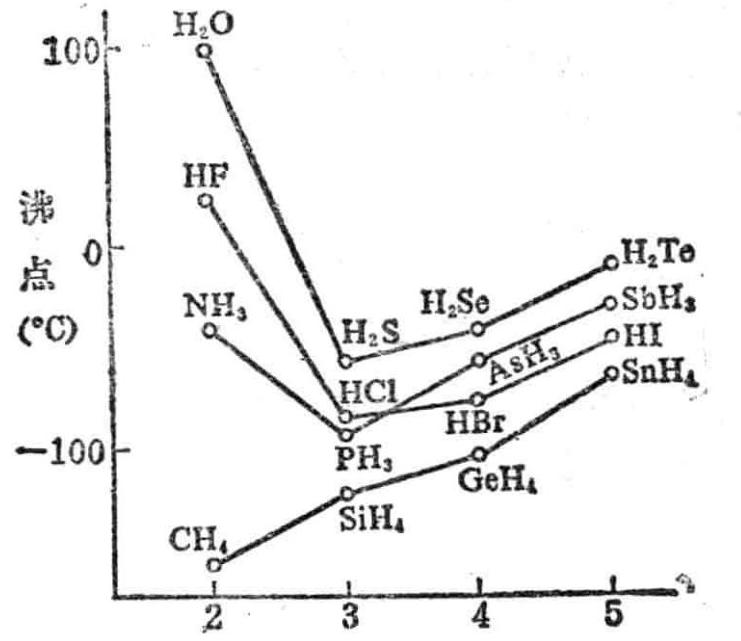
\includegraphics[max width=0.8\textwidth]{images/01912d13-9986-7822-a012-3f3f7be99dcb_28_716816.jpg}
\end{center}

周期 数

图 1-10 一些氢化物的沸点

从表 1-5 和图 1-10 可以看出, 碳族元素的氢化物随着分子量的增大, 沸点逐步增高, 这是符合上节所讲的规律的。但是,在氮族、氧族、卤族的氢化物中, \({\mathrm{{NH}}}_{3}\text{、}{\mathrm{H}}_{2}\mathrm{O}\) 和 \(\mathrm{{HF}}\) 出现沸点反常现象。例如, \(\mathrm{{HF}}\) 的沸点按沸点曲线的下降趋势应 该在 \(- {90}^{ \circ }\mathrm{C}\) 以下,而实际上是 \(+ {20}^{ \circ }\mathrm{C};{\mathrm{H}}_{2}\mathrm{O}\) 的沸点按曲线下降趋势应该在 \(- {70}^{ \circ }\mathrm{C}\) 以下,而实际上是 \(+ {100}^{ \circ }\mathrm{C}\) 。

为什么 \(\mathrm{{HF}}\text{、}{\mathrm{H}}_{2}\mathrm{O}\) 和 \({\mathrm{{NH}}}_{3}\) 出现沸点的反常呢? 这是因为它们的分子之间产生了一种叫做氢键的相互作用, 增加了分子之间的结合力,使得 \(\mathrm{{HF}}\text{、}{\mathrm{H}}_{2}\mathrm{O}\) 和 \({\mathrm{{NH}}}_{3}\) 在较高温度才能气化。

氢键是怎样生成的呢? 现在以 HF 为例来说 明。在 HF 分子中,由于氟的电负性很大, \(\mathrm{H} - \mathrm{F}\) 键的极性很强,共用电子对强烈地偏向 \(\mathrm{F}\) 原子,亦即 \(\mathrm{H}\) 原子的电子云被 \(\mathrm{F}\) 原子吸引, 使 \(\mathrm{H}\) 原子几乎成为 “裸露” 的质子。这个半径很小、带部分正电荷的 \(\mathrm{H}\) 核,允许带部分负电荷的 \(\mathrm{F}\) 原子充分接近它,并产生静电吸引作用,这就形成了氢键。两个 \(\mathrm{F}\) 原子核间的距离为 \(\mathrm{{HF}}\) 分子间氢键的键长。

\begin{center}
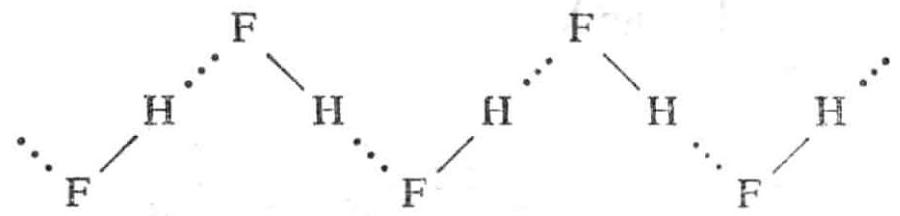
\includegraphics[max width=1.0\textwidth]{images/01912d13-9986-7822-a012-3f3f7be99dcb_29_731384.jpg}
\end{center}

氢键通常用 \(\mathrm{X} - \mathrm{H}\cdots \mathrm{Y}\) 表示,其中 \(\mathrm{X}\) 和 \(\mathrm{Y}\) 代表 \(\mathrm{F}\text{、}\mathrm{O}\text{、}\mathrm{N}\) 等电负性强而原子半径较小的非金属原子。 \(\mathrm{X}\) 和 \(\mathrm{Y}\) 两个核间的距离为氢键的键长。由于在 \(\mathrm{X} - \mathrm{H}\cdots \mathrm{Y}\) 中, \(\mathrm{H}\) 原子只能与一个 \(\mathrm{Y}\) 原子结合; 所以氢键有饱和性。由于 \(\mathrm{X} - \mathrm{H}\) 与 \(\mathrm{Y}\) 原子作用时, \(\mathrm{X} - \mathrm{H}\) 键轴方向尽可能与 \(\mathrm{Y}\) 原子上的孤对电子方向一致, \(\mathrm{X} - \mathrm{H}\cdots \mathrm{Y}\) 中三个原子在同一直线上键最强,所以氢键也有方向性。

氢键的键能在 10 千卡/摩尔以下, 比共价键的键能小得多, 比范德华力稍大一些。分子间氢键的形成使物质的熔点和沸点升高, 这是因为固体熔化或液体气化时必须要破坏分子问的氢键, 要消耗较多的能量。

氢键的强弱跟 \(\mathrm{X}\) 和 \(\mathrm{Y}\) 的电负性有关,它们的电负性越大, 氢键就越强; 又跟 \(\mathrm{Y}\) 的原子半径有关, \(\mathrm{Y}\) 的原子半径越小,越易接近 \(\mathrm{X} - \mathrm{H}\) ,使氢键越强。例如, \(\mathrm{F}\) 原子的电负性最大,半径又很小,因而 \(\mathrm{F} - \mathrm{H}\cdots \mathrm{F}\) 是最强的氢键。 \(\mathrm{{Cl}}\) 原子的电负性虽大,但原子半径大,所以 \(\mathrm{{Cl}} - \mathrm{H}\cdots \mathrm{{Cl}}\) 的氢键很弱。 \(\mathrm{C}\) 原子的电负性较小,一般不形成氢键。这就是为什么 \(\mathrm{{HF}}\text{、}{\mathrm{H}}_{2}\mathrm{O}\) 、 \({\mathrm{{NH}}}_{3}\) 有反常的沸点,而 \(\mathrm{{HCl}}\text{、}{\mathrm{{CH}}}_{4}\) 的沸点却符合范德华力大小的规律的缘故。

在水分子中, \(\mathrm{O}\) 原子的电负性也很强,原子半径较小,所以水分子之间也产生强的氢键。

\begin{center}
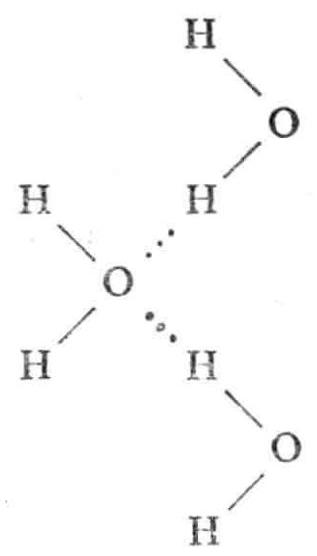
\includegraphics[max width=0.3\textwidth]{images/01912d13-9986-7822-a012-3f3f7be99dcb_30_214898.jpg}
\end{center}

由上式可以看出, 每一水分子中氧原子周围以两个共价键和两个氢键与氢原子结合。

在水蒸气中,水以单个的 \({\mathrm{H}}_{2}\mathrm{O}\) 分子形式存在; 在液态水中,经常是几个水分子通过氢键结合起来,形成 \({\left( {\mathrm{H}}_{2}\mathrm{O}\right) }_{n}\) ; 在固态水(冰)中, 水分子都是以氢键互相联结。可见在水中随着温度的降低, 形成氢键的数目增多。

\section*{习 题}

1. 为什么 \(\mathrm{{HF}}\) 的沸点比 \(\mathrm{{HCl}}\) 和 \(\mathrm{{HBr}}\) 要高出很多?

2. 为什么 \({\mathrm{H}}_{2}\mathrm{O}\) 的沸点比 \({\mathrm{H}}_{2}\mathrm{\;S}\) 和 \({\mathrm{H}}_{2}\mathrm{{Se}}\) 要高出很多?

3. 为什么液态氟化氢的分子式有时写作 \({\left( \mathrm{{HF}}\right) }_{n}\) ?

4. 为什么氨容易液化? 为什么氨容易溶于水?

提示: 氨溶于水形成氢键。

5. 比较氢键和共价键有什么相同和不同点。

\section*{内容提要}

1. 化学键: 在原子结合成分子的时候, 相邻的两个或多个原子之间强烈的相互作用, 通常叫做化学键。

2. 化学键的主要类型有如下几种:

\begin{center}
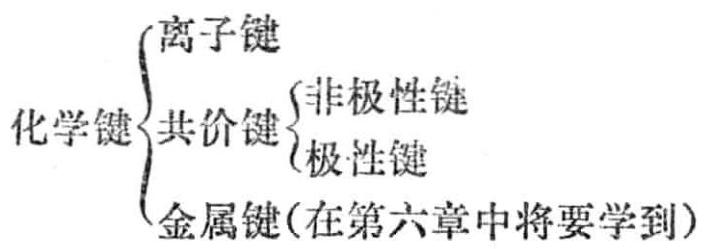
\includegraphics[max width=0.8\textwidth]{images/01912d13-9986-7822-a012-3f3f7be99dcb_31_802703.jpg}
\end{center}

3. 离子键: 阴、阳离子间通过静电作用所形成的化学键叫做离子键。

共价键: 原子间通过共用电子对(电子云重叠)所形成的化学键叫做共价键。共价键具有饱和性和方向性。

(1) 非极性键: 同种原子形成共价键, 共用电子对不偏向任何一个原子, 这样的共价键叫做非极性键。

(2)极性键: 不同种原子形成共价键, 共用电子对偏向吸引电子能力强的原子一方(吸引电子能力大小用电负性来表示), 这样的共价键叫做极性键。

电子对由一个原子单方面提供而跟另一个原子共用的, 这样的共价键叫做配位键。

4. 非极性分子和极性分子

以非极性键组成的分子是非极性分子。

以极性键组成的分子, 如果电荷的空间分布是对称的, 就形成非极性分子; 如果电荷的空间分布是不对称的, 就形成极性分子。

\section*{5. 分子间的作用力}

分子间的作用力又叫范德华力, 按其实质来说是一种电性引力, 它比化学键弱得多, 通常约每摩尔几个千卡。分子间作用力的大小对物质的熔点、沸点、溶解度等有影响。

\section*{6. 氢键}

氢键通常用 \(\mathrm{X} - \mathrm{H}\cdots \mathrm{Y}\) 表示,其中 \(\mathrm{X}\) 和 \(\mathrm{Y}\) 代表 \(\mathrm{F}\text{、}\mathrm{O}\text{、}\mathrm{N}\) 等电负性强而原子半径较小的非金属原子。 氢键的 键 能 在 10 千卡/摩尔以下, 比共价键键能小得多, 比范德华力稍大一些。

\section*{复习题}

1. 试举出一种化合物, 它具有离子键、共价键和配位键。

2. 根据键能数据, 确定下列反应的能量变化是放热的还是吸热的, 能量变化的数值是多少。

(1) \(\mathrm{H} + \mathrm{I} = \mathrm{{HI}}\)

(2) \(\mathrm{{Cl}} + \mathrm{{Cl}} = {\mathrm{{Cl}}}_{2}\)

3. 根据电负性数据分别指出在下列各组化合物中, 哪个键的极性最小, 哪个键的极性最大。

(1) \(\mathrm{{NaCl}}\text{、}{\mathrm{{MgCl}}}_{2}\text{、}{\mathrm{{AlCl}}}_{3}\text{、}{\mathrm{{SiCl}}}_{4}\text{、}{\mathrm{{PCl}}}_{5}\) ,

(2) \(\mathrm{{LiF}}\text{、}\mathrm{{NaF}}\text{、}\mathrm{{KF}}\text{、}\mathrm{{RbF}}\text{、}\mathrm{{CsF}}\) ,

(3) \(\mathrm{{HF}}\text{、}\mathrm{{HCl}}\text{、}\mathrm{{HBr}}\text{、}{\mathrm{{HI}}}_{0}\)

4. 根据下述物质的性质, 试推断它们在固态时属于哪种晶体类型。

(1)晶体硅是硬而脆的固体,熔点 \({1410}^{ \circ }\mathrm{C}\) , 沸点 \({2355}^{ \circ }\mathrm{C}\) , 不溶于一般溶剂。

(2) 硫通常是淡黄色的晶体, 熔点 \({112.8}^{ \circ }\mathrm{C}\) ,沸点 \({444.6}^{ \circ }\mathrm{C}\) , 易溶于二硫化碳中。

(3)氯化钙是无色晶体,熔点 \({782}^{ \circ }\mathrm{C}\) ,沸点 \({1600}^{ \circ }\mathrm{C}\) ,易溶于水, 水溶液能导电。

(4)甲烷是无色气体,熔点是 \(- {182.5}^{ \circ }\mathrm{C}\) ,沸点是 \(- {164}\) \({}^{ \circ }\mathrm{C}\) ,易溶于汽油等有机溶剂。

5. 氯化氢的分子间和甲烷的分子间有没有氢键生成? 为什么? 从它们的什么性质可以推断出来?

6. 说明 \({\mathrm{H}}_{2}\mathrm{O}\) 分子、 \({\mathrm{H}}_{3}{\mathrm{O}}^{ + }\) 离子中化学键的类型。

7. 分析下列物质中各原子间以哪种化学键相结合:

(1) 溴化氢, (2) 氯化钡, (3) 氯化铵, (4) 金刚石, (5) 氨。

8. 如果设想水分子间没有氢键存在, 水的沸点将在怎样的温度范围, 想象一下, 地球上将会有怎样的面貌。

\section*{第二章 氮 族}

\section*{第一节 氮族元素}

元素周期表里第 \(\mathrm{V}\) 主族元素氮 \(\left( \mathrm{N}\right)\) 、磷 \(\left( \mathrm{P}\right)\) 、砷 \(\left( \mathrm{{As}}\right)\) 、锑 (Sb)、铋(Bi), 统称为氮族元素。它们的原子核外电子层排布如表 2-1 所示。

从氮族元素的原子结构来看, 它们原子的最外层电子排布都是 \(n{s}^{2}n{p}^{3}\) ,所以,它们在最高氧化物里的化合价是 +5 价。氮族元素随着原子核外电子层数的增加, 获得电子的趋势逐渐减弱, 失去电子的趋势逐渐增强, 所以, 它们的非金属性逐渐减弱, 金属性逐渐增强。氮、磷表现出比较显著的非金属性, 神虽然是非金属, 但已表现出一些金属性, 而锑、铋已表现出比较明显的金属性。

氮族元素的一些重要性质见表 2-2。

从氮族元素在周期表中的位置来看, 氮族元素的非金属性要比同周期的氧族和卤族元素弱。

本章我们主要学习氮和磷。

表 2-1 氮族元素原子的核外电子层排布

\begin{center}
\adjustbox{max width=\textwidth}{
\begin{tabular}{|c|c|c|c|c|c|c|c|c|c|}
\hline
\multirow{2}{*}{元素名称} & \multirow{2}{*}{元素符号} & \multirow{2}{*}{原子序数} & \multirow{2}{*}{原子} & \multicolumn{6}{|c|}{原子核外电子层排布} \\
\cline{5-10}
& & & & \(\mathrm{K}\) & L & M & \(\mathrm{N}\) & 0 & P \\
\hline
氮 & \(\mathrm{N}\) & 7 & 14.01 & \(1{s}^{2}\) & \(2{s}^{2}2{p}^{8}\) & \phantom{X} & \phantom{X} & \phantom{X} & \phantom{X} \\
\hline
磷 & P & 15 & 30.97 & 1 \({s}^{2}\) & \(2{s}^{2}2{p}^{8}\) & \(3{s}^{2}3{p}^{3}\) & \phantom{X} & \phantom{X} & \phantom{X} \\
\hline
砷 & As & 33 & 74.92 & \(1{s}^{2}\) & \(2{s}^{2}2{p}^{8}\) & \(3{s}^{2}3{p}^{6}3{d}^{10}\) & \(4{s}^{2}4{p}^{3}\) & \phantom{X} & \phantom{X} \\
\hline
锑 & Sb & 51 & 121.8 & \(1{s}^{2}\) & \(2{s}^{2}2{p}^{6}\) & \(3{s}^{2}3{p}^{6}3{d}^{10}\) & \(4{s}^{2}4{p}^{6}4{d}^{10}\) & \(5{s}^{2}5{p}^{3}\) & \phantom{X} \\
\hline
铋 & Bi & 83 & 209.0 & \(1{s}^{2}\) & \(2{s}^{2}2{p}^{6}\) & \(3{s}^{2}3{p}^{6}3{d}^{10}\) & \(4{s}^{2}4{p}^{6}4{d}^{10}4{f}^{14}\) & \(5{s}^{2}5{p}^{6}5{d}^{10}\) & 6. \({s}^{2}\) 6. \({p}^{3}\) \\
\hline
\end{tabular}
}
\end{center}

表 2-2 氮族元素的一些重要性质

\begin{center}
\adjustbox{max width=\textwidth}{
\begin{tabular}{|c|c|c|c|c|c|c|c|}
\hline
\multirow{2}{*}{元素} & \multirow{2}{*}{原子 半径 (10-10 米)} & \multirow{2}{*}{第一电 离 能 (电子 伏特)} & \multirow{2}{*}{主要 化合价} & \multicolumn{4}{|c|}{单} \\
\cline{5-8}
& & & & 狀态 和顏色 & 密 度 (克/厘米 \({}^{3}\) ) & 熔点 \(\left( {{}^{ \circ }\mathrm{C}}\right)\) & 沸点 (℃) \\
\hline
N & 0.75 & 14.53 & \(- 3, + 1\) , \(+ 2, + 3\) , \(+ 4, + 5\) & 无色气体 & 1.2506 (克/升) & \(- {209.86}\) & \(- {195.8}\) \\
\hline
P & 1.10 & 10.484 & \(- 3, + 3\) , \(+ 5\) & 白磷: 白 色或黃色 固体 红磷:暗 红色粉末 & 1. 82 (白磷) 2. 34 (红磷) & 44.1 (白磷) & 280 (白磷) \\
\hline
As & 1.21 & 9.81 & \(- 3, + 3\) , +5 & 灰砷: 灰 色固体 & 5.727 (灰砷) & 817 (28 标 准大气压) (灰砷) & 613 (升华) (灰砷) \\
\hline
Sb & 1.41 & 8.639 & \(+ 3, + 5\) & 银白色 金属 & 6.684 & 630.74 & 1750 \\
\hline
\(\mathrm{{Bi}}\) & 1.52 & 7.287 & \(+ 3, + 5\) & 银白色或 微显红色 金属 & 9.80 & 271.3 & 1560 \\
\hline
\end{tabular}
}
\end{center}

\section*{习 题}

1. 氮族元素包括哪几种元素?分别写出它们的电子排布式。

2. 氮族元素的性质如何随着电子层数的增加而改变?

3. 对比磷酸与硝酸、砷酸 \(\left( {{\mathrm{H}}_{3}{\mathrm{{AsO}}}_{4}, - }\right.\) 种弱酸 \()\) 的酸性; 对比磷酸与硫酸、高氯酸 \(\left( {\mathrm{{HClO}}}_{4}\right)\) 的酸性。

\section*{第二节 氮 气}

氮是一种重要元素, 它以双原子分子存在于大气中, 约占大气总体积的 \({78}\%\) 和质量的 \({75}\%\) 。除了大气是氮的贮藏库外,氮也以化合态形式存在于很多无机物(如硝酸钠和硝酸钾) 和有机物 (如蛋白质和核酸, 二者都是形成生命的重要物质) 中。工业上所用的氮气, 通常是以空气为原料, 将空气液化后, 利用液态空气中液态氮的沸点比液态氧的沸点低而加以分离制得。

\section*{一、氮气的物理性质}

纯净的氮气是一种没有颜色、没有气味的气体, 比空气稍轻 (在标准状况下, 1 升氮气的质量为 1.25 克)。

氮气在 1 标准大气压、 \(- {195.8}^{ \circ }\mathrm{C}\) 时,变成没有颜色的液体, \(- {209.86}^{ \circ }\mathrm{C}\) 时,变成雪状的固体。

氮气在水里的溶解度很小, 在通常状况下, 1 体积水中大约可溶解 0.02 体积的氮气。

\section*{二、氮气的化学性质}

\begin{center}
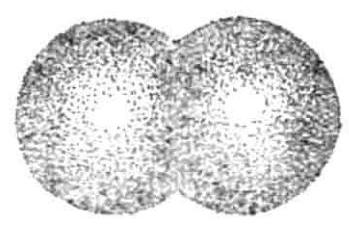
\includegraphics[max width=0.4\textwidth]{images/01912d13-9986-7822-a012-3f3f7be99dcb_37_708916.jpg}
\end{center}

图 2-1 氮分子示意图

氮分子是由两个氮原子共用三对电子结合而成的分子(图 2- 1), 氮分子中有三个共价键:

: N :: N : \(\;N \equiv N\)

它的键能很大 (226.3 千卡/摩尔), 大于其它双原子分子(如氢分子的键能为 104.2 千卡/摩尔, 氧分子的键能为 118.86 千卡/摩尔), 因而氮分子的结构很稳定。在通常情况下, 氮气的性质很不活泼, 很难跟其它物质发生化学反应。但在高温下, 氮分子获得了足够的能量, 促使它的共价键断裂, 就能跟氢、 氧、金属等物质发生化学反应。

\section*{1. 氮气跟氢气的反应}

氮气跟氢气在高温、高压并有催化剂存在的条件下, 可以直接化合生成氨 \(\left( {\mathrm{{NH}}}_{3}\right)\) 。

\[
{\mathrm{N}}_{2} + 3{\mathrm{H}}_{2}\underset{\text{ 催化剂 }}{\overset{\text{ 高温、高压 }}{ \rightleftharpoons }}2{\mathrm{{NH}}}_{3} + {22.08}\text{ 千卡 }
\]

工业上就是利用这个反应原理来合成氨的。

\section*{2. 氮气跟氧气的反应}

在放电条件下, 氮气跟氧气能直接化合生成无色的一氧化氮(NO)。

\[
{\mathrm{N}}_{2} + {\mathrm{O}}_{2}\xrightarrow[]{\text{ 放电 }}2\mathrm{{NO}}
\]

一氧化氮不溶于水, 在常温下很容易跟空气中的氧气化合,生成棕色并有刺激性气味的二氧化氮 \(\left( {\mathrm{{NO}}}_{2}\right)\) 。

\[
2\mathrm{{NO}} + {\mathrm{O}}_{2} = 2{\mathrm{{NO}}}_{2}
\]

因此在闪电时, 大气中常有少量的二氧化氮产生。

二氧化氮有毒, 易溶于水。它溶于水后生成硝酸和一氧化氮。

\[
3{\mathrm{{NO}}}_{2} + {\mathrm{H}}_{2}\mathrm{O} = 2{\mathrm{{HNO}}}_{3} + \mathrm{{NO}}
\]

二氧化氮还可相互化合成无色的四氧化二氮 \(\left( {{\mathrm{N}}_{2}{\mathrm{O}}_{4}}\right)\) 气体。

\[
\text{2 NO2 (无色) (无色)}
\]

一氧化氮和二氧化氮是两种重要的氮的氧化物。氮的氧化物除这两种外,还有一氧化二氮 \(\left( {{\mathrm{N}}_{2}\mathrm{O}}\right)\) 、三氧化二氮 \(\left( {{\mathrm{N}}_{2}{\mathrm{O}}_{3}}\right)\) 、 四氧化二氮 \(\left( {{\mathrm{N}}_{2}{\mathrm{O}}_{4}}\right)\) 、五氧化二氮 \(\left( {{\mathrm{N}}_{2}{\mathrm{O}}_{5}}\right)\) 等,可见氮跟氧化合时,在不同条件下,它能生成不同的氧化物。氮在 \({\mathrm{N}}_{2}\mathrm{O}\text{、}\mathrm{{NO}}\) 、 \({\mathrm{N}}_{2}{\mathrm{O}}_{3}\text{、}{\mathrm{{NO}}}_{2}\text{、}{\mathrm{\;N}}_{2}{\mathrm{O}}_{5}\) 这五种不同的氧化物里,其化合价分别是 \(+ 1\text{、} + 2\text{、} + 3\text{、} + 4\text{、} + 5\) 价,氮的最高化合价是 +5 价。

\section*{3. 氮气跟某些金属的反应}

在高温的时候, 氮气能够跟镁、钙、锶、钡等金属化合。例如, 镁在空气里燃烧时, 除跟氧气化合生成氧化镁外, 也能跟氮气化合生成微量的氮化镁 \(\left( {{\mathrm{{Mg}}}_{3}{\mathrm{\;N}}_{2}}\right)\) 。

\[
3\mathrm{{Mg}} + {\mathrm{N}}_{2} = \frac{\text{ 点燃 }}{}{\mathrm{{Mg}}}_{3}{\mathrm{\;N}}_{2}
\]

\section*{三、氮的固定}

把大气中的氮转化为氮的化合物叫做氮的固定。上文所述, 在闪电时大气中有氮的氧化物生成, 这是自然界的一种氮的固定过程。豆科作物的根部常附有小根瘤, 其中含有能使空气中氮气在常温常压下转化为硝酸盐的固氮菌。这种转化是自然界的又一种氮的固定过程。

工业上用氮气合成氨, 以及在放电条件下制备氮的氧化物, 再合成硝酸, 这是人工氮的固定过程。

氮化合物的天然矿藏是很少的, 而燃料的燃烧、有机物的腐败, 又常使氮化合物分解生成氮气进入大气中。面临对氮的化合物的庞大需要(氮肥、炸药、染料、合成纤维等都需用氮的化合物作原料), 当前研究人工氮的固定是十分重要的。

\section*{四、氮气的用途}

大量的氮气在工业上用作合成氨的原料, 从氨又可以制备各种氮肥和硝酸。因此, 氮气也是一种重要的化工原料。由于氮气的化学性质不活泼, 氮气可用来代替惰性气体作焊接金属时的保护气; 氮气或氮气和氩气的混和气体可用来充填灯泡, 以防止钨丝的氧化和减慢钨丝的挥发, 使灯泡经久耐用。粮食、水果如处于低氧高氮的环境中, 能使害虫缺氧窒息而死, 同时能使植物种子处于休眠状态, 代谢缓慢, 所以可利用氮气保存粮食、水果等农副产品。

\section*{习 题}

1. 为什么在常温下氮气不容易跟其它物质起反应而 在高温下却能起反应?

2. 使含有硫化氢和水蒸气的空气, 依次通过氢氧化钠溶液、浓硫酸和灼热的铜丝, 最后所得的气体含有哪些成分? 为什么? 写出有关反应的化学方程式。

3. 五个集气瓶里分别装有下列各种气体: 氯气、氧气、 氮气、二氧化碳和二氧化硫。根据哪些性质鉴别它们: 写出有关反应的化学方程式。

4. 怎样鉴别二氧化氮和溴蒸气?

\section*{第三节 氨 铵盐}

\section*{一、氨}

\section*{1. 氨分子的结构}

氮原子的最外电子层有 5 个电子,电子排布式是 \(2{s}^{2}2{p}^{3}\) , 在氨分子中,氮原子的 3 个未成对的 \({2p}\) 电子分别与 3 个氢原子中的 \({1s}\) 电子形成共用电子对,也就是说,氮以三个共价键与三个氢原子联结:

\begin{center}
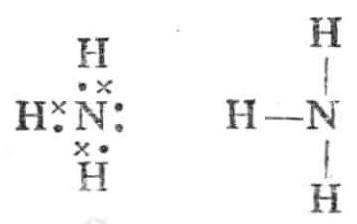
\includegraphics[max width=0.4\textwidth]{images/01912d13-9986-7822-a012-3f3f7be99dcb_41_254205.jpg}
\end{center}

氨分子中的 \(\mathrm{N} - \mathrm{H}\) 键是极性键。 经实验测定, 氨分子的结构呈三角锥形, 氮原子位于锥顶, 三个氢原子位于锥底, \(\mathrm{N} - \mathrm{H}\) 键之间的键角为 \({107}^{ \circ }{18}^{\prime }\) , 所以说氨分子是一个极性分子 (图 2- 2)。

\begin{center}
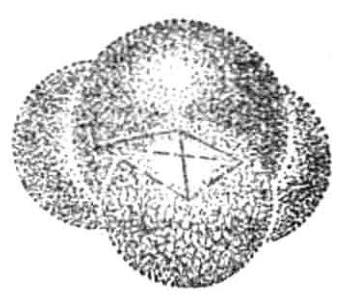
\includegraphics[max width=0.4\textwidth]{images/01912d13-9986-7822-a012-3f3f7be99dcb_41_738932.jpg}
\end{center}

图 2-2 氨分子结构示意图

\section*{2. 氨的物理性质}

氨是没有颜色、具有刺激性气味的气体。在标准状况下, 氨的密度是 0.771 克/升, 比同体积的空气轻。

由于氨分子中氢原子是与电负性很大而原子半径较小的氮原子以共价键结合的, 因而如同水分子一样, 氨分子之间也可形成氢键。由于氢键的形成, 氨分子间的引力增强, 使氨很容易液化。在常压下冷却到 \(- {33.35}^{ \circ }\mathrm{C}\) 或在常温下加压到7- 8 个标准大气压, 气态氨就凝结为无色的液体, 同时放出大量的热。液态氨气化时要吸收大量的热, 而使它周围温度急剧降低, 因此, 氨常用作致冷剂。

氨极易溶解于水。在常温下, 1 体积水约可溶解 700 体积氨, 氨的水溶液叫做氨水。

\section*{3. 氨的化学性质}

\section*{(1) 氨跟水的反应}

[实验 2-1] 在干燥的圆底烧瓶里充满氨气, 用带有玻璃管和滴管(滴管里预先吸入水)的塞子塞紧瓶口。立即倒置烧瓶, 使玻璃管插入盛有水的烧杯 (水里事先加入少量酚酞溶液), 挤压滴管的胶头, 使少量水进入烧瓶。烧杯里的水即由玻璃管喷入烧瓶, 形成红色的喷泉(图 2-3)。

\begin{center}
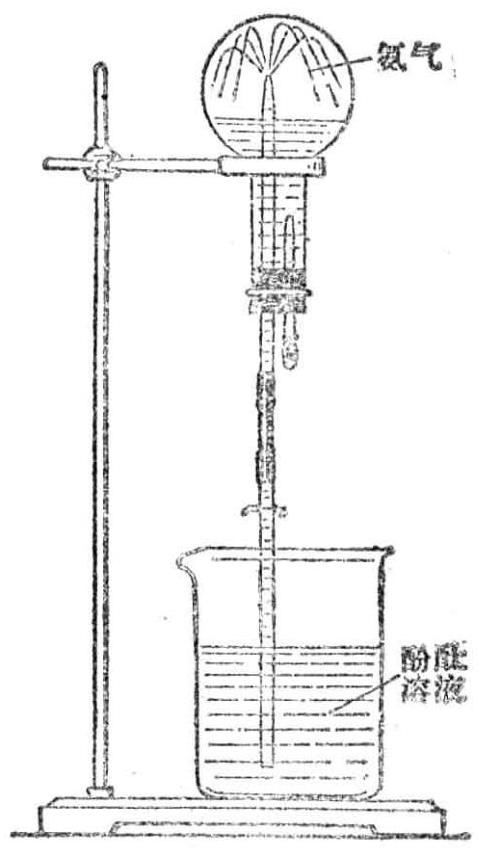
\includegraphics[max width=0.5\textwidth]{images/01912d13-9986-7822-a012-3f3f7be99dcb_42_903538.jpg}
\end{center}

图 2-3 氨易溶于水

实验表明, 氨极易溶于水, 大量氨溶于水后, 烧瓶里的压强迅速减小, 这时外界的大气压就把烧杯里的水迅速压上去。 形成了喷泉。同时, 可以看到这含有少量酚酞的水变成红色。 表明氨水具有碱性。

根据加热浓氨水时有氨气逸出, 以及氨水在低温时能析出氨的结晶水合物一一水合氨 \(\left( {{\mathrm{{NH}}}_{3} \cdot {\mathrm{H}}_{2}\mathrm{O}}\right)\) 的实验事实,可知氨溶于水中,大部分与水 结合 成一水合氨 \(\left( {{\mathrm{{NH}}}_{3} \cdot {\mathrm{H}}_{2}\mathrm{O}}\right)\) , \({\mathrm{{NH}}}_{3} \cdot {\mathrm{H}}_{2}\mathrm{O}\) 是由氨分子和水分子通过氢键结合起来的。

一水合氨很不稳定, 受热就会分解而生成氨和水:

\[
{\mathrm{{NH}}}_{3} \cdot {\mathrm{H}}_{2}\mathrm{O}\overset{\bigtriangleup }{ \leftrightharpoons }{\mathrm{{NH}}}_{3} \uparrow + {\mathrm{H}}_{2}\mathrm{O}
\]

一水合氨可以小部分电离成 \({\mathrm{{NH}}}_{4}{}^{ + }\) 和 \({\mathrm{{OH}}}^{ - }\) ,所以氨水显弱碱性, 能使酚酞溶液变红色。氨在水中的反应可用下式表示:

\[
{\mathrm{{NH}}}_{3} + {\mathrm{H}}_{2}\mathrm{O} \rightleftharpoons {\mathrm{{NH}}}_{3} \cdot {\mathrm{H}}_{2}\mathrm{O} \rightleftharpoons {\mathrm{{NH}}}_{4}{}^{ + } + {\mathrm{{OH}}}^{ - }
\]

也可简单表示如下:

\[
{\mathrm{{NH}}}_{3} + {\mathrm{H}}_{2}\mathrm{O} \rightleftharpoons {\mathrm{{NH}}}_{4}{}^{ + } + {\mathrm{{OH}}}^{ - }
\]

\section*{(2) 氨跟酸的反应}

[实验 2-2] 拿一根玻璃棒在浓氨水里蘸一下, 另一根玻璃棒在浓盐酸里蘸一下, 使这两根玻璃棒接近 (不要接触), 就有大量的白烟产生 (图 2-4)。

\begin{center}
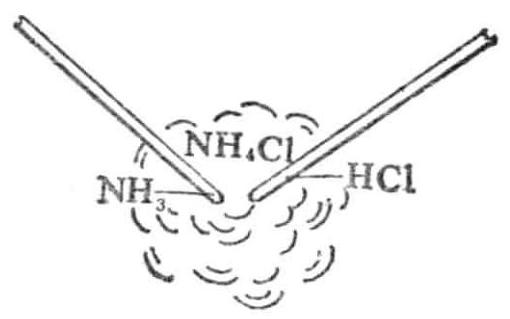
\includegraphics[max width=0.6\textwidth]{images/01912d13-9986-7822-a012-3f3f7be99dcb_43_436028.jpg}
\end{center}

图 2-4 氨跟氯化氢反应

这白烟是氨水里挥发出的氨跟浓盐酸挥发出的氯化氢化合所生成的微小的氯化铵晶体:

\[
{\mathrm{{NH}}}_{3} + \mathrm{{HCl}} = {\mathrm{{NH}}}_{4}\mathrm{{Cl}}
\]

氨興靜能跟其它的酸化合生成铵盐。如把氨通入硝酸或硫酸中, 就会生成硝酸铵或硫酸铵:

\[
{\mathrm{{NH}}}_{3} + {\mathrm{{HNO}}}_{3} = {\mathrm{{NH}}}_{4}{\mathrm{{NO}}}_{3}
\]

\[
2{\mathrm{{NH}}}_{3} + {\mathrm{H}}_{2}{\mathrm{{SO}}}_{4} = {\left( {\mathrm{{NH}}}_{4}\right) }_{2}{\mathrm{{SO}}}_{4}
\]

\section*{(3)氨跟氧气的反应}

在催化剂(如铂、氧化铁、氧化铬等)存在的情况下, 氨跟氧气发生如下的反应:

\[
4{\mathrm{{NH}}}_{3} + 5{\mathrm{O}}_{2}\frac{\text{ 催化剂 }}{\Delta }4\mathrm{{NO}} + 6{\mathrm{H}}_{2}\mathrm{O} + {216.7}\text{ 千卡 }
\]

[实验 2-3] 慢慢把空气通入盛浓氨水的锥形瓶中, 再将红热的螺旋状铂丝 \(O\) 接近液面,但不要使铂丝跟氨水接触 (图 2-5)。可观察到锥形瓶中有棕色气体生成 \(\Phi\) ,这是因为氨被氧化为一氧化氮, 后者再遇氧气生成二氧化氮。同时, 还可观察到铂丝继续保持红热, 这是因为氨分子跟氧分子在铂丝表面上进行的这个反应是放热的。

\begin{center}
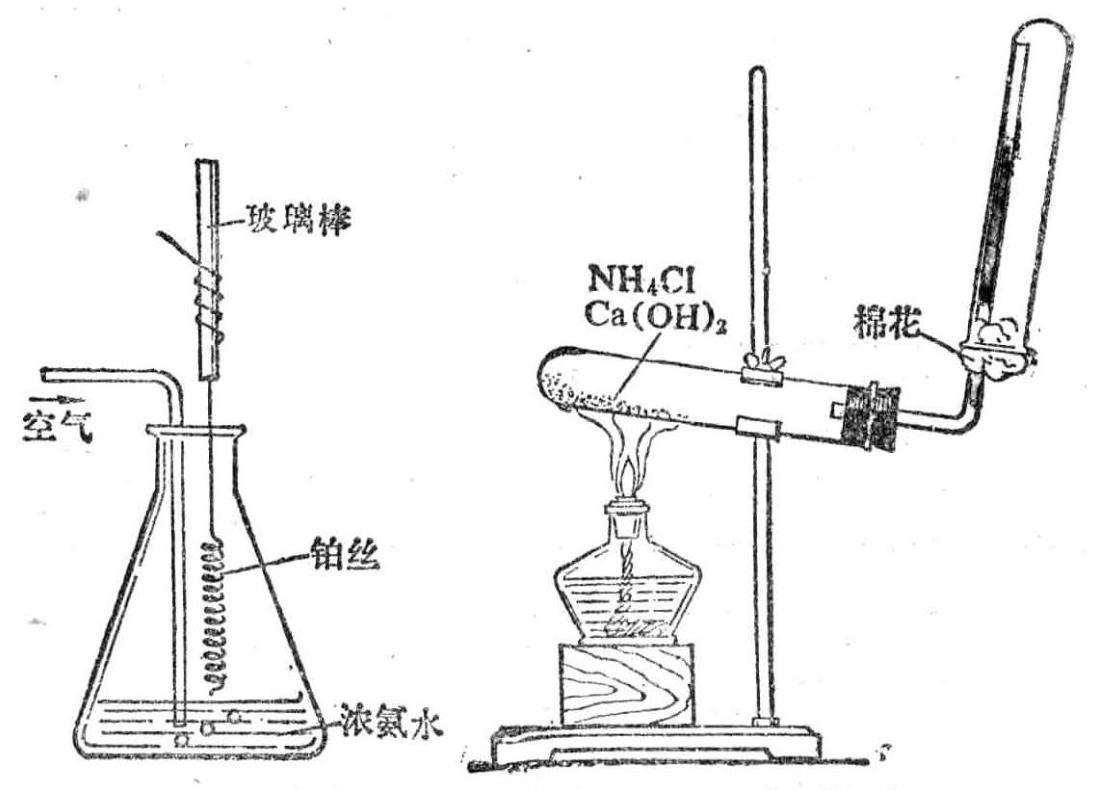
\includegraphics[max width=1.0\textwidth]{images/01912d13-9986-7822-a012-3f3f7be99dcb_44_234942.jpg}
\end{center}

图 2-5 氨的催化氧化 图 2-6 氨的制取

\customfootnote{

① 用加热 \({\left( {\mathrm{{NH}}}_{4}\right) }_{2}{\mathrm{{Cr}}}_{2}{\mathrm{O}}_{7}\) 新制得的 \({\mathrm{{Cr}}}_{2}{\mathrm{O}}_{3}\) 代替铂丝作催化剂,实验效果也很明显。

}

上述反应叫做氨的催化氧化(或叫接触氧化), 它是工业上制硝酸的基础。

\section*{4. 氨的实验室制法}

在实验室里常用给铵盐和碱加热的方法来制取氨。

\[
2{\mathrm{{NH}}}_{4}\mathrm{{Cl}} + \mathrm{{Ca}}{\left( \mathrm{{OH}}\right) }_{2} \triangleq {\mathrm{{CaCl}}}_{2} + 2{\mathrm{{NH}}}_{3} \uparrow + 2{\mathrm{H}}_{2}\mathrm{O}
\]

[实验 2-4] 给试管里的氯化铵和消石灰的混和物加热, 用倒立的干燥的试管收集氨 (图 2-6)。把润湿的红色石蕊试纸放在试管口, 观察试纸颜色的变化, 可以试验氨是否已经充满试管。

实验室中要制取干燥的氨,通常使制得的氨通过碱石灰 \({}^{\left( 2\right) }\) ,以吸收其中的水蒸气。

\section*{5. 氨的用途}

氨是一种重要的化工产品。它不仅是氮肥工业的基础, 同时又是制造硝酸、铵盐、纯碱等的重要原料。 氨在有机合成工业 (如合成纤维、塑料、染料等) 里也是一种常用的原料。 氨又是一种常用的致冷剂。

\customfootnote{

① 由于锥形瓶里有水蒸气存在, 它跟二氧化氮起反应生成硝酸, 硝酸再跟氨起反应生成硝酸铵晶体。因此,锥形瓶里常看到有白烟 \({J}^{zz}\) 生。

② 在氢氧化钠浓溶液中加入氧化钙, 加热, 制成白色固体即得碱石灰, 它是水分和二氧化碳的吸收剂。

}

[讨论].

(1) 液氨与氨水有什么不同? 在氨水里有哪些分子和离子?

(2)氨和铵有什么不同?

\section*{二、铵盐}

氨跟酸作用可生成铵盐。铵盐是由铵离子 \(\left( {{\mathrm{{NH}}}_{4}{}^{ + }}\right)\) 和酸根离子组成的化合物。

铵盐都是晶体, 能溶解于水。铵盐的化学性质如下:

1. 铵盐受热分解

[实验 2-5] 给试管里的氯化铵晶体加热, 观察发生的现象 (图 2-7)。

\begin{center}
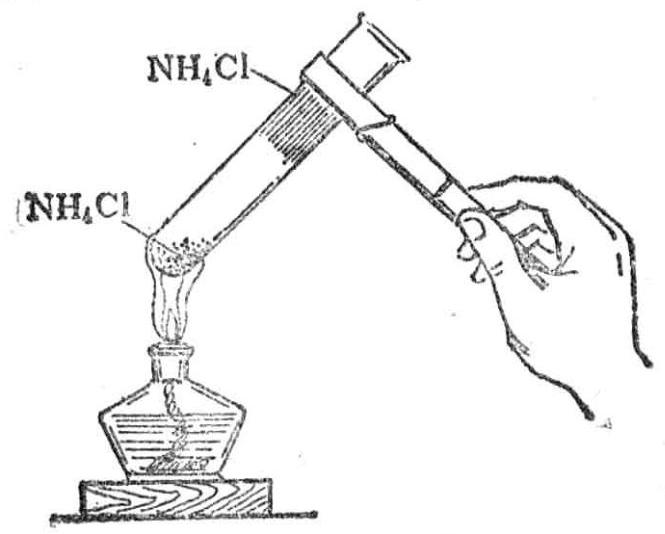
\includegraphics[max width=0.7\textwidth]{images/01912d13-9986-7822-a012-3f3f7be99dcb_46_347795.jpg}
\end{center}

图 2-7 氯化铵受热分解

受热时, 氯化铵分解生成氨和氯化氢, 冷却时, 它们又重新结合生成氯化铵。

\[
{\mathrm{{NH}}}_{4}\mathrm{{Cl}} \triangleq {\mathrm{{NH}}}_{3} \uparrow + \mathrm{{HCl}} \uparrow
\]

\[
{\mathrm{{NH}}}_{3} + \mathrm{{HCl}} = {\mathrm{{NH}}}_{4}\mathrm{{Cl}}
\]

碳酸氢铵受热时, 分解生成氨、水和二氧化碳。

\[
{\mathrm{{NH}}}_{4}{\mathrm{{HCO}}}_{3} \triangleq {\mathrm{{NH}}}_{3} \uparrow + {\mathrm{H}}_{2}\mathrm{O} + {\mathrm{{CO}}}_{2} \uparrow
\]

铵盐受热容易分解, 分解时, 一般放出氨。

\section*{2. 铵盐跟碱的反应}

铵盐能跟碱起反应放出氨气。例如:

\({\left( {\mathrm{{NH}}}_{4}\right) }_{2}{\mathrm{{SO}}}_{4} + 2\mathrm{{NaOH}}\overset{\bigtriangleup }{ = }{\mathrm{{Na}}}_{2}{\mathrm{{SO}}}_{4} + 2{\mathrm{{NH}}}_{3} \uparrow + 2{\mathrm{H}}_{2}\mathrm{O}\)

这个性质是一切铵盐的通性。实验室里就利用这样的反应来制取氨, 同时也可以利用这个性质来检验铵离子的存在。

铵盐在工农业生产上有着重要的用途。大量的铵盐用作氮肥。硝酸铵还用来制炸药。氯化铵常用作印染和制干电池的原料, 它也用在金属的焊接上, 以除去金属表面上的氧化物薄层。

\section*{习 题}

1. 浓硫酸常用作气体的干燥剂, 是否可用来干燥氨气? 为什么?

2. 碘受热变成蒸气, 碘蒸气遇冷变成碘; 氯化铵受热分解生成的气体遇冷仍变成氯化铵, 这两种现象本质上是否相同? 为什么?

3. 怎样用化学方法证明硫酸铵既是铵盐又是硫酸盐? 写出检验方法、现象和有关的化学方程式。

4. 制备 1 升含氨 10\% 的氨水(密度是 0.96 克/厘米 \({}^{3}\) ) 需要用多少体积的氨气(标准状况下)?

5. 350 体积 (标准状况下) 的氨溶解在 1 体积的水里, 这种氨水的百分比浓度是多少?摩尔浓度是多少?【这种氨水的密度是 0.924 克/厘米 \({}^{3}\) )

6. 用氢氧化钙和氯化铵各 10 克, 在标准状况下可以制得多少升的氨气? 如果把这些氨配成 500 毫升的氨水, 这种溶液的摩尔浓度是多少?

\section*{第四节 硝酸的工业制法}

硝酸是一种重要的化工产品, 它是制造炸药、染料、塑料、 硝酸盐和许多其它化工产品的重要原料。

现代生产硝酸最重要的方法是氨的催化氧化法, 这个方法的生产过程大致可分为两个阶段: (1) 氨氧化生成一氧化氮; (2)一氧化氮氧化生成二氧化氮, 二氧化氮被水(或稀硝酸)吸收而生成硝酸。

\begin{center}
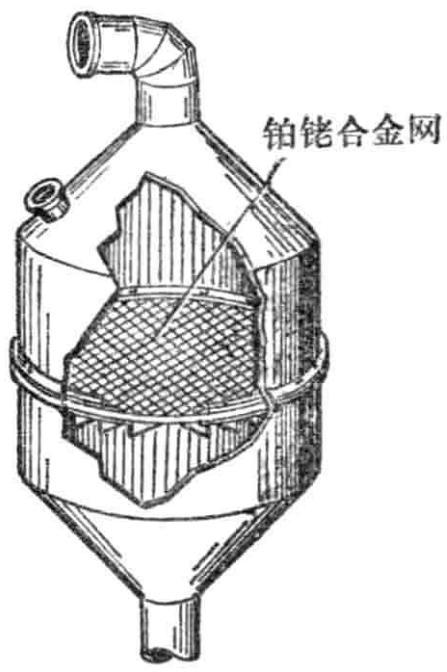
\includegraphics[max width=0.5\textwidth]{images/01912d13-9986-7822-a012-3f3f7be99dcb_48_912596.jpg}
\end{center}

图 2-8 氧化炉 \(\rbrack\)

\section*{1. 氨的氧化}

将氨和净化后的空气以一定比混和,进入氧化炉 (图 2-8)。 氧化炉的中部有多层水平的铂铑合金网作为催化剂,在 \({800}^{ \circ }\mathrm{C}\) 的高温下, 氨跟氧气在网上进行反应生成一氧化氮和水蒸气, 同时放出大量的热。

\[
4{\mathrm{{NH}}}_{3} + 5{\mathrm{O}}_{2}\frac{\mathrm{{Pt}} - \mathrm{{Rh}}}{\text{ 高温 }}4\mathrm{{NO}} + 6{\mathrm{H}}_{2}\mathrm{O}
\]

\(+ {216.7}\) 千卡

2. 硝酸的生成

一氧化氮经过冷却, 再被空气中的氧氧化成二氧化氮。

\[
2\mathrm{{NO}} + {\mathrm{O}}_{2} = 2{\mathrm{{NO}}}_{2} + {27.02}\text{千卡}
\]

最后, 在吸收塔内二氧化氮被水吸收, 就得到了硝酸。

\[
3{\mathrm{{NO}}}_{2} + {\mathrm{H}}_{2}\mathrm{O} = 2{\mathrm{{HNO}}}_{3} + \mathrm{{NO}} + {32.5}\text{千卡}
\]

从这一反应看,只有 \(2/3\) 的二氧化氮转化为硝酸,而 \(1/3\) 的二氧化氮转化为一氧化氮。因此, 常在吸收反应进行过程中补充一些空气, 使生成的一氧化氮再氧化为二氧化氮, 二氧化氮溶于水又生成硝酸和一氧化氮。经过这样多次的氧化和吸收, 二氧化氮可以比较完全地被水吸收, 能够尽可能多地转化为硝酸。

从吸收塔出来的尾气中尚含有少量未被吸收的一氧化氮和二氧化氮, 如果不加处理就排放到空气中, 会造成污染, 严重危害人体健康及农作物生长。为消灭氮的氧化物对大气的污染, 变废为宝, 将尾气通入碱液吸收塔, 用碱液吸收, 可制得重要的化工原料亚硝酸钠:

\[
\mathrm{{NO}} + {\mathrm{{NO}}}_{2} + 2\mathrm{{NaOH}} = 2{\mathrm{{NaNO}}}_{2} + {\mathrm{H}}_{2}\mathrm{O}
\]

用上述方法制得的硝酸的浓度一般为 \({50}\%\) 左右,如果要制取更浓的硝酸, 可用硝酸镁 (或浓硫酸) 作为吸水剂, 将稀硝酸蒸馏浓缩,就可以得到 \({96}\%\) 以上的浓硝酸。

\section*{习 题}

1. 简述氨氧化制取硝酸的化学反应原理, 并写出有关反应的化学方程式。

2. 雷雨时, 雨水里可含有微量的硝酸。人们曾模拟自然界的这一过程, 用电弧法生产硝酸。当空气通过电极之间的它弧时,极高的温度,导致氮气氧化为一氧化氮。但即使在 \({3000}^{ \circ }\mathrm{C}\) 的高温,也只能生成 \(5\%\) (按体积计)的 \(\mathrm{{NO}}\) 。由于耗电多, 产率低, 这个方法已逐渐被其它方法代替。试写出用电弧法生产硝酸的有关的化学方程式。

3. 氨氧化制硝酸时, 如果由氨制成一氧化氮的产率是 \({96}\%\) ,由一氧化氮制成硝酸的产率是 \({92}\%\) 。10 吨氨可以制备多少吨 50\% 的硝酸?

4. 制备 \({6M}{\mathrm{{HNO}}}_{3}\) 溶液 250 毫升,问需用 \({65.3}\%\) 的浓硝酸(密度是 1.4 克/厘米 \({}^{3}\) ) 多少毫升?

\section*{第五节 硝酸 硝酸盐}

\section*{一、硝酸}

\section*{1. 硝酸的物理性质}

纯硝酸是无色、易挥发、有刺激性气味的液体, 密度为 1.5027 克/厘米 \({}^{3}\) ,沸点 \({83}^{ \circ }\mathrm{C}\) ,凝固点 \(- {42}^{ \circ }\mathrm{C}\) 。它能以任意比溶解于水。常用的浓硝酸的浓度大约是 \({69}\%\) 。浓度为 \({98}\%\) 以上的浓硝酸在空气里由于硝酸的挥发而产生“发烟”现象,通常叫做发烟硝酸。这是因为硝酸里放出的硝酸蒸气遇到空气里的水蒸气生成了极微小的硝酸液滴的缘故。

\section*{2. 硝酸的化学性质}

硝酸是一种强酸。它除了具有酸的通性以外, 还有它本身的特性。

(1) 硝酸的不稳定性

硝酸很不稳定, 容易分解。纯净的硝酸或浓硝酸在常温下见光就会分解, 受热时分解得更快。

\[
4{\mathrm{{HNO}}}_{3}\frac{\bigtriangleup }{\text{ 或光照 }}2{\mathrm{H}}_{2}\mathrm{O} + 4{\mathrm{{NO}}}_{2} \uparrow + {\mathrm{O}}_{2} \uparrow
\]

硝酸越浓, 就越容易分解。分解放出的二氧化氮溶于硝酸而使硝酸呈黄色。为了防止硝酸分解, 必须把它盛在棕色瓶里, 贮放在黑暗而且温度低的地方。

\section*{(2)硝酸的氧化性}

硝酸是一种很强的氧化剂, 不论稀硝酸还是浓硝酸都有氧化性, 几乎能跟所有的金属(除金、铂等少数金属外)或非金属发生氧化-还原反应。

[实验 2-6] . 在放有铜片的两个试管里, 分别加入少量浓硝酸和稀硝酸, 观察现象。

浓硝酸和稀硝酸都能跟铜起反应。前者反应激烈, 有红棕色的气体产生; 后者反应较缓慢, 有无色气体产生, 在试管口变红棕色。

以上反应的化学方程式分别是:

\[
\mathrm{{Cu}} + 4{\mathrm{{HNO}}}_{3}\text{(浓)} = \mathrm{{Cu}}{\left( {\mathrm{{NO}}}_{3}\right) }_{2} + 2{\mathrm{{NO}}}_{2} \uparrow + 2{\mathrm{H}}_{2}\mathrm{O}
\]

\[
3\mathrm{{Cu}} + 8{\mathrm{{HNO}}}_{3}\text{ (稀) } = 3\mathrm{{Cu}}{\left( {\mathrm{{NO}}}_{3}\right) }_{2} + 2\mathrm{{NO}} \uparrow + 4{\mathrm{H}}_{2}\mathrm{O}
\]

从上述两个反应可以看出: 硝酸跟金属发生反应时, 主要是正五价的氮得到电子, 被还原成较低价的氮的化合物, 并不象盐酸跟较活泼金属反应那样放出氢气。除金、铂等少数几种金属外, 硝酸几乎可以使所有的金属氧化而生成硝酸盐。

值得注意的是,有些金属如铝、铁等常温下在浓硝酸中会发生钝化现象。这是因为浓硝酸将它们的表面氧化成一层薄而致密的氧化物薄膜, 因而阻止了进一步反应的缘故。所以, 可以用铝槽车装盛浓硝酸。

浓硝酸和浓盐酸的混和物(摩尔比 1:3) 叫做王水, 它的氧化能力更强, 能使一些不溶于硝酸的金属, 如金、铂等溶解。

硝酸还能使许多非金属(如碳、硫、磷)及某些有机物(如松节油、锯末等)氧化。例如:

\[
4{\mathrm{{HNO}}}_{3} + \mathrm{C} = 2{\mathrm{H}}_{2}\mathrm{O} + 4{\mathrm{{NO}}}_{2} \uparrow + {\mathrm{{CO}}}_{2} \uparrow
\]

\section*{3. 硝酸的实验室制法}

硝酸有挥发性, 所以, 在实验室里可以把硝酸盐跟浓硫酸共同加热来制取它。

\[
{\mathrm{{NaNO}}}_{3} + {\mathrm{H}}_{2}{\mathrm{{SO}}}_{4}\text{(浓)} \triangleq {\mathrm{{NaHSO}}}_{4} + {\mathrm{{HNO}}}_{3} \uparrow
\]

\section*{二、硝酸盐}

多数硝酸盐是无色晶体, 极易溶于水。硝酸盐性质不稳定, 加热易分解放出氧气, 所以, 在高温时硝酸盐是强氧化剂。

[实验 2-7] 给试管里的硝酸钾加热到熔融, 把带有火星的细木条伸进试管口检验放出的气体, 同时观察放出气体的颜色和试管中剩余物的颜色。

分别用硝酸铜、硝酸银晶体代替硝酸钾, 做上面的实验。

从实验可知, 各种硝酸盐加热后都会分解, 一般地说, 在金属活动性顺序表里镁以前的比较活泼金属的硝酸盐, 加热时放出氧气并生成亚硝酸盐。例如:

\[
2{\mathrm{{KNO}}}_{3} \triangleq 2{\mathrm{{KNO}}}_{2} + {\mathrm{O}}_{2} \uparrow
\]

在金属活动性顺序表里位于镁和铜之间的金属的硝酸盐, 在加热时, 生成金属氧化物、二氧化氮和氧气。例如:

\[
2\mathrm{{Cu}}{\left( {\mathrm{{NO}}}_{3}\right) }_{2} \triangleq 2\mathrm{{CuO}} + 4{\mathrm{{NO}}}_{2} \uparrow + {\mathrm{O}}_{2} \uparrow
\]

活动性很小的金属的硝酸盐, 即在金属活动性顺序表里铜以后的金属的硝酸盐, 在加热时生成金属单质、二氧化氮和氧气。例如:

\[
2{\mathrm{{AgNO}}}_{3} \triangleq 2\mathrm{{Ag}} + 2{\mathrm{{NO}}}_{2} \uparrow + {\mathrm{O}}_{2} \uparrow
\]

由于硝酸盐是氧化剂, 所以, 用硝酸钾和易燃的硫粉、炭粉可配制成黑色火药。

\section*{义沟}

1. 硝酸和硫酸、盐酸的性质有什么相同的地方和不同的地方?怎样用实验方法来鉴别这三种酸?

2. 依次写出下列变化的化学方程式, 并注明反应发生的条件。

\[
{\mathrm{N}}_{2} \rightarrow {\mathrm{{NH}}}_{3} \rightarrow \mathrm{{NO}} \rightarrow {\mathrm{{NO}}}_{2} \rightarrow {\mathrm{{HNO}}}_{3} \rightarrow {\mathrm{{NH}}}_{4}{\mathrm{{NO}}}_{3}
\]

3. 把铜片放到下列各种酸里各有什么现象发生? 能起反应的写出化学方程式, 不能起反应的说明理由。

(1)稀盐酸, (2) 浓硫酸, (3) 稀硫酸, (4) 浓硝酸, (5)稀硝酸。

4. \({3.5}\mathrm{M}\) 的稀硝酸溶液 50 毫升与足量的铜起反应,生成多少克硝酸铜? 计算生成的一氧化氮在标准状况下的体积。

5. 写出下列四种硝酸盐受热分解的化学方程式:

\[
{\mathrm{{NaNO}}}_{3}\text{、}\mathrm{{Ca}}{\left( {\mathrm{{NO}}}_{3}\right) }_{2}\text{、}\mathrm{{Fe}}{\left( {\mathrm{{NO}}}_{3}\right) }_{3}\text{、}\mathrm{{Hg}}{\left( {\mathrm{{NO}}}_{3}\right) }_{2}。
\]

6. \({62}\%\) 的硝酸溶液 (密度为 1.38 克/厘米 \({}^{3}\) ) 的摩尔浓度是多少? 若将这种浓硝酸 100 毫升稀释至 500 毫升, 求它的摩尔浓度是多少?

7. 给硝酸钠晶体跟浓硫酸和铜共热, 将会发生什么现象?用这种方法可以鉴定硝酸盐吗?对于很稀的硝酸盐溶液用这种方法鉴定行不行?

\section*{第六节 氧化-还原反应方程式的配平}

在初中化学里, 我们学过一些氧化-还原反应, 这些氧化- 还原反应的化学方程式比较简单, 反应物和生成物的系数是较小的整数, 不难通过观察来配平。但是, 在高中化学里已经学到的或以后将会学到的较复杂的氧化-还原反应, 如硝酸跟金属或非金属的反应等, 就不容易用观察的方法来配平它们的化学方程式。那么, 这些复杂的化学方程式怎样配平呢?

我们知道, 氧化-还原反应的本质是参加反应的原子间的电子转移(包括电子得失和电子对的偏移), 原子间的电子转移可以用元素的化合价的升降来表示。因此, 氧化-还原反应的化学方程式可以通过分析电子转移或化合价升降来配平。 在这里, 我们学习用化合价升降的方法来配平化学方程式。

[例题1] 配平铜跟稀硝酸反应的化学方程式。

[解] 1. 先写出反应物和生成物的分子式, 并列出发生氧化和还原的元素的正负化合价。

\[
\mathrm{{Cu}} + {\mathrm{{HNO}}}_{3} - - \mathrm{{Cu}}{\left( {\mathrm{{NO}}}_{3}\right) }_{2} + \overset{+2}{\mathrm{{NO}}} + {\mathrm{H}}_{2}\mathrm{O}
\]

2. 列出元素的化合价的变化。

\begin{center}
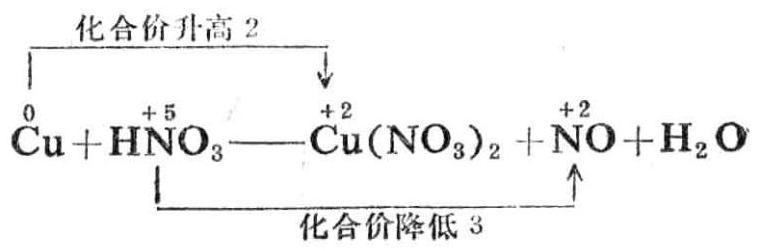
\includegraphics[max width=0.8\textwidth]{images/01912d13-9986-7822-a012-3f3f7be99dcb_55_983090.jpg}
\end{center}

3. 使化合价的升高和降低的总数相等。

\begin{center}
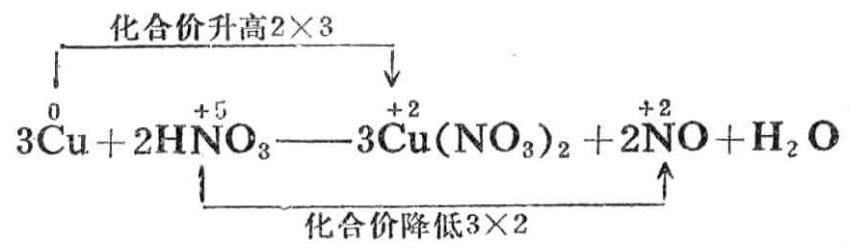
\includegraphics[max width=0.9\textwidth]{images/01912d13-9986-7822-a012-3f3f7be99dcb_55_289451.jpg}
\end{center}

4. 用观察的方法配平其它物质的系数。在上述反应里, 有 6 个 \({\mathrm{{NO}}}_{3}\) -没有参与氧化-还原反应,所以 \({\mathrm{{HNO}}}_{3}\) 的系数应是 \(8;{\mathrm{H}}_{2}\mathrm{O}\) 的系数应是 4,因为有 2 个 \({\mathrm{{NO}}}_{3}{}^{ - }\) 还原成 \(\mathrm{{NO}}\) ,其中 4 个氧原子跟 \({\mathrm{{HNO}}}_{3}\) 中氢离子结合成水。配平后,把单线改成等号。

\[
3\mathrm{{Cu}} + 8{\mathrm{{HNO}}}_{3}\text{ (稀) } = 3\mathrm{{Cu}}{\left( {\mathrm{{NO}}}_{3}\right) }_{2} + 2\mathrm{{NO}} \uparrow + 4{\mathrm{H}}_{2}\mathrm{O}
\]

[例题 2] 配平碳跟硝酸起反应的化学方程式。

[解] 1. 写出反应物和生成物的分子式, 列出发生氧化-还原反应的元素的正负化合价。

\[
\mathrm{C} + {\mathrm{{HNO}}}_{3} - {\mathrm{{NO}}}_{2} + {\mathrm{{CO}}}_{2} + {\mathrm{H}}_{2}\mathrm{O}
\]

2. 列出元素的化合价变化。

\begin{center}
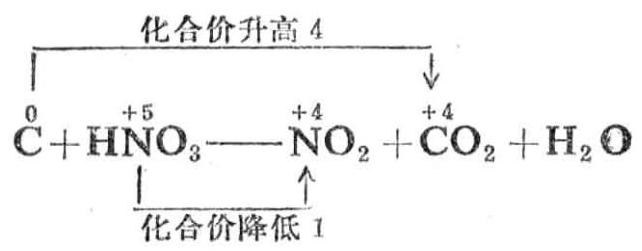
\includegraphics[max width=0.7\textwidth]{images/01912d13-9986-7822-a012-3f3f7be99dcb_55_630813.jpg}
\end{center}

3. 使化合价的升高和降低的总数相等。

\begin{center}
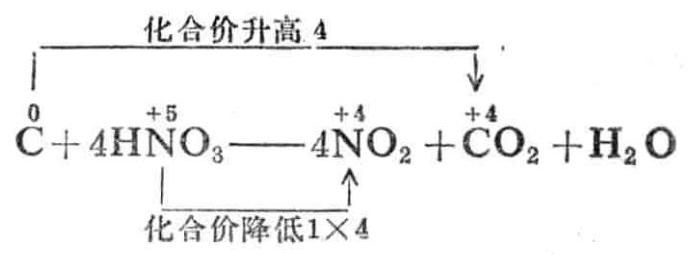
\includegraphics[max width=0.8\textwidth]{images/01912d13-9986-7822-a012-3f3f7be99dcb_56_435659.jpg}
\end{center}

4. 配平其它物质的系数, 把单线改成等号。

\[
\mathrm{C} + 4{\mathrm{{HNO}}}_{3} = 4{\mathrm{{NO}}}_{2} \uparrow + {\mathrm{{CO}}}_{2} \uparrow + 2{\mathrm{H}}_{2}\mathrm{O}
\]

\section*{习 题}

1. 配平下列氧化-还原反应的化学方程式, 并指出哪种元素被氧化了, 哪种元素被还原了。

(1) \({\mathrm{{SO}}}_{2} + {\mathrm{O}}_{2} - {\mathrm{{SO}}}_{3}\)

(2) \(\cdot \mathrm{P} + {\mathrm{{Cl}}}_{2} - {\mathrm{{PCl}}}_{3}\)

(3) \(\mathrm{{NaBr}} + {\mathrm{{Cl}}}_{2} - \mathrm{{NaCl}} + {\mathrm{{Br}}}_{2}\)

(4) \(\mathrm{{Fe}} + {\mathrm{{FeCl}}}_{3} - {\mathrm{{FeCl}}}_{2}\)

(5) \({\mathrm{{KClO}}}_{3} - \mathrm{{KCl}} + {\mathrm{O}}_{2}\)

2. 配平下列氧化-还原反应的化学方程式。

(1) \(\mathrm{{Cu}} + {\mathrm{H}}_{2}{\mathrm{{SO}}}_{4}\) (浓) \(- {\mathrm{{CuSO}}}_{4} + {\mathrm{{SO}}}_{2} + {\mathrm{H}}_{2}\mathrm{O}\)

(2) \({\mathrm{{MnO}}}_{2} + \mathrm{{HCl}}\) (浓) \(- {\mathrm{{MnCl}}}_{2} + {\mathrm{{Cl}}}_{2} + {\mathrm{H}}_{2}\mathrm{O}\)

(3) \({\mathrm{{NH}}}_{3} + {\mathrm{O}}_{2} - \mathrm{{NO}} + {\mathrm{H}}_{2}\mathrm{O}\)

(4) \({\mathrm{{NO}}}_{2} + {\mathrm{H}}_{2}\mathrm{O} - {\mathrm{{HNO}}}_{3} + \mathrm{{NO}}\)

(5) \(\mathrm{{Mg}} + {\mathrm{{HNO}}}_{3}\) (稀) \(- \mathrm{{Mg}}{\left( {\mathrm{{NO}}}_{3}\right) }_{2} + {\mathrm{{NH}}}_{4}{\mathrm{{NO}}}_{3} + {\mathrm{H}}_{2}\mathrm{O}\)

3. 配平过氧化钠跟二氧化碳的反应。

\[
{\mathrm{{Na}}}_{2}{\mathrm{O}}_{2} + {\mathrm{{CO}}}_{2} - {\mathrm{{Na}}}_{2}{\mathrm{{CO}}}_{3} + {\mathrm{O}}_{2}
\]

(提示: 过氧化钠中氧元素的化合价是 -1 , 在反应中, 一个氧原子从 -1 降为 -2, 另一个氧原子从 -1 升为 0 。)

\section*{第七节 磷 磷酸 磷酸盐}

\section*{一、磷}

由同种元素组成的不同性质的单质叫做同素异形体。磷有多种同素异形体, 其中最重要的是白磷和红磷。

\section*{1. 磷的物理性质}

白磷是一种蜡状的固体, 有剧毒, 不溶于水, 但能溶于二硫化碳里。把白磷隔绝空气加热到 \({260}^{ \circ }\mathrm{C}\) ,就会转变成红磷。红磷是暗红色粉末状的固体, 没有毒, 不溶于水, 也不溶于二硫化碳。红磷加热到 \({416}^{ \circ }\mathrm{C}\) 时就升华,它的蒸气冷却后变成白磷。

\section*{2. 磷的化学性质}

磷的化学性质活泼, 容易跟氧、卤素以及许多金属直接化合。

(1)磷跟氧的化合反应

[实验 2-8] 把一块铁片水平地夹在铁架上, 把少量的白磷和红磷隔开相当的距离分放在铁片上 (图 2-9), 然后在红磷的下面加热, 观察是红磷还是白磷先着火燃烧。

\begin{center}
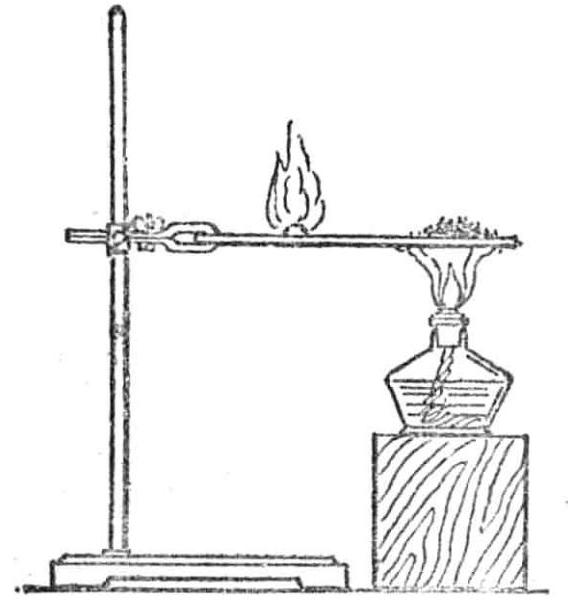
\includegraphics[max width=0.6\textwidth]{images/01912d13-9986-7822-a012-3f3f7be99dcb_57_701972.jpg}
\end{center}

图 2-9 白磷和红磷的着火点的比较

实验说明白磷远比红磷容易燃烧。白磷的着火点是 \({40}^{ \circ }\mathrm{C}\) , 红磷的着火点是 \({240}^{ \circ }\mathrm{C}\) 。白磷受到轻微的摩擦或被加热到 \({40}^{ \circ }\mathrm{C}\) ,就会发生燃烧现象。所以,白磷必须贮存在密闭容器里, 少量的白磷可保存在水里。

白磷和红磷的着火点虽然不同, 但是燃烧以后, 都生成五氧化二磷。五氧化二磷极易吸水, 是一种强干燥剂。

白磷在空气里, 即使在常温下, 也会缓慢地氧化, 氧化时会发光, 在暗处可以清楚地看见。

磷跟氮一样, 在它的氧化物和氯化物里的最高化合价是 +5 , 在它跟氢和金属的化合物里, 化合价是一 3 。

\section*{(2) 磷跟卤素化合}

由于卤素的电负性比磷高, 因此, 磷在其卤化物中显示 \(+ 3\) 和 +5 价。磷在不充足的氯气中燃烧生成三氯化磷。

\[
2\mathrm{P} + 3{\mathrm{{Cl}}}_{2}\xrightarrow[]{\text{ 点燃 }}2{\mathrm{{PCl}}}_{3}
\]

在过量的氯气中燃烧生成五氯化磷。

\[
2\mathrm{P} + 5{\mathrm{{Cl}}}_{2}\xrightarrow[]{\text{ 点燃 }}2{\mathrm{{PCl}}}_{5}
\]

白磷和红磷在性质上的差别, 是由于它们具有不同的结构引起的。白磷分子是由四个磷原子结合而成的 \({\mathrm{P}}_{4}\) 分子,4 个磷原子排布在一个正四面体的 4 个顶角上, 每个磷原子与分子中的其他 3 个磷原子以共价键相结合(图 2-10)。而红磷的结构远比白磷复杂, 这里就不作介绍了。

\begin{center}
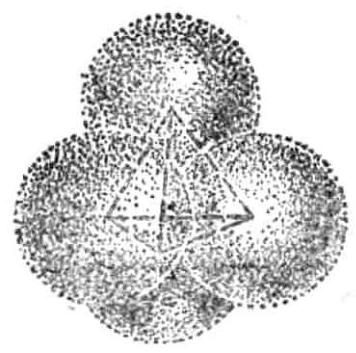
\includegraphics[max width=0.4\textwidth]{images/01912d13-9986-7822-a012-3f3f7be99dcb_58_455439.jpg}
\end{center}

图 2-10 白磷分子结构示意图

\section*{3. 磷的存在和用途}

磷在空气中易被氧化, 因此自然界里没有游离态的磷存在。磷主要以磷酸盐的形式存在于矿石中。此外动物的骨骼、 牙齿、脑髓和神经组织里都含有磷。植物的果实和幼芽里也含有磷。磷对于维持生物体正常的生活机能有重要的作用。

白磷可用于制造纯度高的磷酸; 红磷除用于制农药外, 主要用于制造安全火柴。火柴盒侧面所涂的物质就是红磷和三硫化二锑等的混和物,而火柴头上的物质一般是氧化剂 (氯酸钾、二氧化锰) 和易燃物如硫等。当两者摩擦时, 因摩擦而生的热使跟氯酸钾接触的红磷发火, 并引起火柴头上的易燃物燃烧, 从而使火柴杆着火。此外, 在军事上还用磷来制造烟幕弹和燃烧弹。

\section*{二、磷酸和磷酸盐}

五氧化二磷极易与水化合, 发生剧烈反应, 同时放出大量的热。随着反应条件的不同,可生成偏磷酸 \(\Phi \left( {\mathrm{{HPO}}}_{3}\right)\) 或磷酸 \(\left( {{\mathrm{H}}_{3}{\mathrm{{PO}}}_{4}}\right)\) :

\[
{\mathrm{P}}_{2}{\mathrm{O}}_{5} + {\mathrm{H}}_{2}\mathrm{O}\xrightarrow[]{\text{ 冷水 }}2{\mathrm{{HPO}}}_{3}
\]

\[
{\mathrm{P}}_{2}{\mathrm{O}}_{5} + 3{\mathrm{H}}_{2}\mathrm{O}\xrightarrow[]{\text{ 热水 }}2{\mathrm{H}}_{3}{\mathrm{{PO}}}_{4}
\]

磷酸是无色透明的晶体,熔点为 \({42.35}^{ \circ }\mathrm{C}\) ,具有吸湿性,易溶于水, 和水能以任何比混和。通常用的磷酸是一种无色粘稠的浓溶液,内含 \({83} - {98}\%\) 的纯磷酸。

\customfootnote{

① 从一分子磷酸脱去一分子水而成的酸, 称为偏磷酸。

\[
{\mathrm{H}}_{3}{\mathrm{{PO}}}_{4} = {\mathrm{{HPO}}}_{3} + {\mathrm{H}}_{2}\mathrm{O}
\]

磷酸 偏磷酸

}

磷酸没有毒, 而偏磷酸则有剧毒。

磷酸比硝酸稳定, 不易分解。工业上是用硫酸跟磷酸钙反应来制取磷酸的:

\[
{\mathrm{{Ca}}}_{3}{\left( {\mathrm{{PO}}}_{4}\right) }_{2} + 3{\mathrm{H}}_{2}{\mathrm{{SO}}}_{4}\overset{\bigtriangleup }{ = }2{\mathrm{H}}_{3}{\mathrm{{PO}}}_{4} + 3{\mathrm{{CaSO}}}_{4} \downarrow
\]

滤去硫酸钙沉淀, 所得滤液就是磷酸溶液。

磷酸不显氧化性, 是一种中等强度的三元酸。它能形成三种类型的盐, 一种正盐和两种酸式盐。例如:

磷酸二氢盐 \({\mathrm{{NaH}}}_{2}{\mathrm{{PO}}}_{4}\mathrm{{Ca}}{\left( {\mathrm{H}}_{2}{\mathrm{{PO}}}_{4}\right) }_{2}{\mathrm{{NH}}}_{4}{\mathrm{H}}_{2}{\mathrm{{PO}}}_{4}\)

磷酸氢盐 \({\mathrm{{Na}}}_{2}{\mathrm{{HPO}}}_{4}{\mathrm{{CaHPO}}}_{4}\;{\left( {\mathrm{{NH}}}_{4}\right) }_{2}{\mathrm{{HPO}}}_{4}\)

磷酸盐 \(\;{\mathrm{{Na}}}_{3}{\mathrm{{PO}}}_{4}\;{\mathrm{{Ca}}}_{3}{\left( {\mathrm{{PO}}}_{4}\right) }_{2}\;{\left( {\mathrm{{NH}}}_{4}\right) }_{3}{\mathrm{{PO}}}_{4}\)

所有的磷酸二氢盐都易溶于水, 而磷酸氢盐和磷酸盐中除钾、钠和铵盐外, 几乎都不溶于水。

磷酸盐大量用于磷肥。自然界的磷矿石的主要成分是磷酸钙, 它是难溶于水的矿物。化学工业上制造磷肥的目的, 就是加工磷矿石, 使它们由难溶于水的正盐转化为较易溶于水 (或弱酸)的酸式盐, 以利于植物吸收。

\section*{习 题}

1. 白磷和红磷在性质上有何不同?怎样证明白磷和红磷是同素异形体? 白磷是哪种类型的晶体?

2. 怎样分别用下列两种物质为原料来制备磷酸: (1) 磷, (2)磷酸钙。如果要制备 500 克磷酸, 需要磷、磷酸钙各多少克? 制备过程中的化学反应是否都属于氧化-还原反应?

3. 现有 \({2.4M}{\mathrm{H}}_{3}{\mathrm{{PO}}}_{4}\) 溶液 500 毫升,需要分别加入多少一

毫升 \({3M}\mathrm{{NaOH}}\) 溶液才能把反应物中所含 \({\mathrm{H}}_{3}{\mathrm{{PO}}}_{4}\) 全部转化为: (1) 磷酸二氢钠, (2)磷酸氢二钠, (3)磷酸钠。

4. 当 26.4 克的硫酸铵跟过量的氢氧化钠一起加热时, 放出的气体全部被含 39.2 克磷酸的溶液所吸收。这时生成的盐是什么?

5. 写出下列物质依次变化的化学方程式:

\[
\mathrm{P} \rightarrow {\mathrm{P}}_{2}{\mathrm{O}}_{5} \rightarrow {\mathrm{H}}_{3}{\mathrm{{PO}}}_{4} \rightarrow {\mathrm{{Ca}}}_{3}{\left( {\mathrm{{PO}}}_{4}\right) }_{2} \rightarrow \mathrm{{Ca}}{\left( {\mathrm{H}}_{2}{\mathrm{{PO}}}_{4}\right) }_{2}
\]

\section*{内容提要}

\section*{一、氮族元素}

氮族元素属于元素周期表的第 \(\mathrm{V}\) 主族,包括氮、磷、 砷、锑、铋五种元素。氮族元素原子的最外电子层的排布为 \(n{s}^{2}n{p}^{3}\) ,其非金属性比同周期的氧族、卤族元素弱。

\section*{二、氮气}

1. 由于氮分子 \(\left( { : \mathrm{N}\vdots \vdots \mathrm{N} : }\right)\) 的键能很大,结构稳定,在常温下它很不活泼。但在高温下, 氮分子也能跟氢气、氧气、金属等许多物质起化学反应。

2. 氮有很多氧化物, 其中一氧化氮和二氧化氮是两种重要的氮的氧化物。

\section*{三、氨和铵盐}

1. 氨分子的结构呈三角锥形, 它是极性分子。由于氨分子间可形成氢键, 所以氨容易液化; 由于氨分子与水分子间可形成氢键, 所以氨极易溶于水。

2. 氨水具有弱碱性, 氨溶于水发生下列反应:

\[
{\mathrm{{NH}}}_{3} + {\mathrm{H}}_{2}\mathrm{O} \rightleftharpoons {\mathrm{{NH}}}_{3} \cdot {\mathrm{H}}_{2}\mathrm{O} \rightleftharpoons {\mathrm{{NH}}}_{4}{}^{ + } + {\mathrm{{OH}}}^{ - }
\]

3. 氨跟酸反应生成铵盐。

4. 铵盐受热易分解。

5. 铵盐跟碱起反应: \({\mathrm{{NH}}}_{4}{}^{ + } + {\mathrm{{OH}}}^{ - }\overset{\Delta }{ = }{\mathrm{{NH}}}_{3} \uparrow + {\mathrm{H}}_{2}\mathrm{O}\) 实验室利用这个反应来检验铵离子 \(\left( {{\mathrm{{NH}}}_{4}{}^{ + }}\right)\) 的存在。

\section*{四、硝酸和硝酸盐}

1. 硝酸除具有酸的通性外, 还具有以下特性:

(1)不稳定性。见光受热易分解。

(2)氧化性。硝酸是一种很强的氧化剂,它几乎能跟所有的金属(除金、铂外)、非金属发生氧化-还原反应。

2. 氨氧化法制硝酸的化学反应大致可分为两个阶段, 即氮催化氧化生成一氧化氮; 一氧化氮氧化生成二氧化氮, 二氧化氮被水吸收生成硝酸。

3. 硝酸盐性质不稳定, 受热易分解放出氧气, 所以在高温下也是强氧化剂。

\section*{五、磷、磷酸和磷酸盐}

1. 磷有多种同素异形体, 其中最重要的是白磷和红磷。

2. 磷能够跟氧气、卤素等直接化合。

3. 磷酸是一种中等强度的三元酸, 比硝酸稳定, 不易分解。

4. 磷酸能形成三种类型的盐: 正盐、氢盐和二氢盐。

\section*{六、用化合价升降的方法来配平氧化-还原反应方程式}

先写出反应物和生成物的分子式, 并列出发生氧化或还原的元素的正负化合价, 再列出元素的化合价变化并使化合价的升高和降低的总数相等, 最后用观察的方法配平其它物质的系数。

\section*{复习题}

1. 解释下列现象:

(1)为什么浓硝酸常放在棕色的瓶子里?

(2)锌跟稀硫酸反应可产生氢气,而跟稀硝酸反应则没有氢气放出。

(3) 铜溶于稀硝酸, 而不溶于稀硫酸。

2. 有一种白色晶体, 它跟氢氧化钠共热的时候, 放出一种无色气体, 这种气体能使润湿的红色石蕊试纸变蓝; 跟浓硫酸共热的时候, 也放出一种无色气体, 这种气体能使润湿的蓝色石蕊试纸变红。如果这两种气体相遇会发生白烟。原来的白色晶体可能是什么物质? 写出上述有关反应的化学方程式。

3. 怎样利用空气和水为原料来制造硝酸铵? 写出制造过程中有关反应的化学方程式并注明反应条件。

4. 硝酸铜可以用下列三种方法制备:铜跟浓硝酸起反应, 铜跟稀硝酸起反应, 氧化铜跟硝酸起反应。如果用这三种方法制取等量的硝酸铜, 消耗的纯硝酸的质量是否相等? 哪一种用掉的硝酸最少?

5. 根据下列氮元素化合价的变化, 写出实现各步变化的化学方程式,并分别指出 \(\left( 1\right) \text{、}\left( 4\right)\) 两步变化中什么物质是还原剂?

\begin{center}
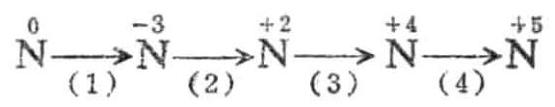
\includegraphics[max width=0.6\textwidth]{images/01912d13-9986-7822-a012-3f3f7be99dcb_64_557691.jpg}
\end{center}

6. 氯化钠和氯化铵在性质上有什么相似的地方?怎样从氯化铵和氯化钠的混和物里把氯化铵分离出来?

7. 有五瓶白色固体: 硝酸钠、硫酸铵、碳酸钙、氯化铵、磷酸钠, 你用什么化学方法把它们分别检验出来? 写出实验操作步骤和产生的现象, 以及它们的化学方程式。

8. 某一种气态氮的氧化物 250 毫升 (在标准状况下), 质量为 0.33 克,它的组成里含氧 \({53.5}\%\) ,求它的分子式。

9. 取铜银合金 1 克, 放入硝酸中溶解, 再加盐酸, 则得氯化银沉淀 0.35 克, 求此合金中铜、银的百分率各多少?

10. 把 10 毫升一氧化氮和二氧化氮的混和气体通入倒立在水槽的盛满水的量筒里,片刻以后,量筒里留下 5 毫升气体。 计算通入的混和气体里, 一氧化氮和二氧化氮各几毫升。

11. 配平下列氧化-还原反应的化学方程式:

(1) \({\mathrm{{KMnO}}}_{4} + \mathrm{{HCl}} - - {\mathrm{{MnCl}}}_{2} + \mathrm{{KCl}} + {\mathrm{H}}_{2}\mathrm{O} + {\mathrm{{Cl}}}_{2}\)

(2) \({\mathrm{{FeS}}}_{2} + {\mathrm{O}}_{2} - {\mathrm{{Fe}}}_{2}{\mathrm{O}}_{3} + {\mathrm{{SO}}}_{2}\)

\section*{第三章 化学反应速度和}

化学平衡

我们已经学习了一些化学反应, 知道化学反应往往需要在一定的条件下进行, 例如, 上章讲到使氢气和氮气化合生成氨时, 就要在高温、高压和有催化剂存在的条件下进行。为什么一个反应的进行需要这样或那样的条件呢? 这就要从以下两个方面来认识: 一个是反应进行的快慢, 即化学反应速度问题; 一个是反应进行的程度, 也就是达到化学平衡的问题。 这两个问题不仅是今后学习化学所必需的基础理论知识, 也是研究化工生产适宜条件时需要掌握的化学变化的规律。

\section*{第一节 化学反应速度}

\section*{一、化学反应速度}

各种化学反应的进行有快有慢, 如氢、氧爆鸣气的爆炸反应、酸碱溶液的中和反应等瞬时就能完成; 而石油的形成就要经过亿万年。这里所说的快和慢, 是指在一定条件下进行的化学反应。只要掌握了化学反应的规律, 我们就可以根据科学研究、生产和生活的需要, 采取适当的措施, 把原来进行得很慢的反应加快, 如加速炼钢过程, 加速合成树脂或合成橡胶的反应等; 或把原来进行得快的反应减慢, 如钢铁的防锈, 塑料、橡胶的防止老化等等。这些对发展生产, 节约支出, 促进社会主义现代化建设, 都具有重要的意义。

怎样来衡量化学反应速度的大小呢?

通常对于某些反应可以通过观察反应物的消失速度和生成物的出现速度作出对这个反应速度的定性判断。例如, 当把一条镁带放在一个盛稀盐酸的烧杯里, 在镁带(反应物)迅速消失的同时, 会很快地放出氢气(生成物)。当在同浓度的盐酸中放入铁块时, 铁块以较慢速度消失, 同时氢气放出的速度也较缓慢。显然第一个反应的速度比第二个反应大得多。

怎样定量地较准确地表示化学反应速度呢? 化学反应的速度是用单位时间 (如每秒、每分或每小时等)内反应物或生成物的量 (摩尔) 的变化来表示, 通常是用单位时间内反应物浓度的减小或生成物浓度的增大来表示。浓度的单位一般为摩尔/升, 反应速度的单位就是摩尔/升·分或摩尔/升·秒等。

例如: 某一反应物的浓度是 2 摩尔/升, 经过两分钟的反应后, 它的浓度变成了 1.8 摩尔/升, 即两分钟后反应物的浓度减小了 0.2 摩尔/升, 这就是说, 在这两分钟内它的平均反应速度为 0.1 摩尔/升·分。

\section*{二、影响反应速度的条件}

不同的化学反应, 具有不同的反应速度。例如, 酸和碱的中和反应, 就比氮分子跟氢分子合成氨的反应快得多, 这说明参加反应物质的性质是决定化学反应速度的主要因素。但是外界条件对化学反应速度也有一定的影响, 就是同一个化学反应, 如浓度、压强、温度、催化剂等外界条件不同时, 反应速度也不相同。下面我们来研究影响化学反应速度的几个重要条件。

\section*{1. 浓度对化学反应速度的影响}

我们在初中学习氧的性质时, 曾看到硫在空气中缓慢燃烧并产生微弱的淡蓝色火焰, 在纯氧中迅速燃烧并发出明亮的蓝紫色火焰。这说明硫在纯氧中跟氧化合的反应比在空气中的反应进行得更快、更剧烈。这是因为纯氧中氧分子的浓度比空气中氧分子的浓度大的缘故。从下面的实验可以看出, 在溶液中进行的反应也是这样的情况。

[实验 3-1] 取两个试管,在第一个试管中加入 \({0.1}\mathrm{M}\) \({\mathrm{{Na}}}_{2}{\mathrm{\;S}}_{2}{\mathrm{O}}_{3}\) (硫代硫酸钠) 溶液 10 毫升; 在第二个试管中加入 \({0.1M}{\mathrm{{Na}}}_{2}{\mathrm{\;S}}_{2}{\mathrm{O}}_{3}\) 溶液和蒸馏水各 5 毫升。

另取两个试管,每个试管加入 \({0.1M}{\mathrm{H}}_{2}{\mathrm{{SO}}}_{4}\) 溶液各 10 毫升。然后同时分别倒入上面两个盛有 \({\mathrm{{Na}}}_{2}{\mathrm{\;S}}_{2}{\mathrm{O}}_{3}\) 溶液的试管中, 并注意观察两个盛有混和溶液试管里出现浑浊现象的先后。

实验结果表明: 首先出现浑浊现象的是第一个试管, 接着才是第二个试管。

通过许多实验证明, 当其它条件不变时, 增加反应物的浓度, 可以增大反应的速度。

\section*{2. 压强对化学反应速度的影响}

对于气体来说, 当温度一定时, 一定量气体的体积与其所受的压强成反比。这就是说, 如果气体的压强增大到原来的两倍, 气体的体积就缩小到原来的一半, 单位体积内的分子数就增多到原来的两倍, 如图 3-1 所示。所以, 增大压强, 就, 是增加单位体积里反应物的摩尔数, 即是增大反应物的浓度, 因而可以增大反应的速度。相反, 减小压强, 气体的体积就扩大, 浓度减小, 因而反应速度减小。

\begin{center}
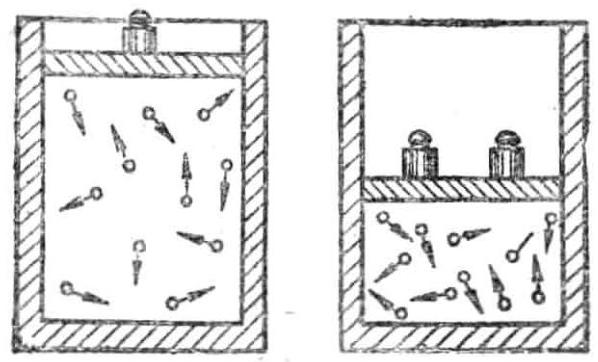
\includegraphics[max width=0.6\textwidth]{images/01912d13-9986-7822-a012-3f3f7be99dcb_68_697520.jpg}
\end{center}

图 3-1 压强大小与一定量分子所占体积的示意图

如果参加反应的物质是固体、液体或溶液时, 由于改变压强对它们的体积改变很小, 因而对它们的浓度改变很小, 可以认为压强与它们的反应速度无关。

\section*{3. 温度对化学反应速度的影响 活化能}

我们知道, 许多化学反应都是在加热的情况下发生的。例如, 在常温下煤在空气里甚至在纯氧里不能燃烧, 只有加热到一定温度时才能燃烧, 并且越燃越旺。物质在溶液里进行的反应也有类似的情况。

[实验 3-2] 取两个试管,在每个试管中各加入 \({0.1M}\) \({\mathrm{{Na}}}_{2}{\mathrm{\;S}}_{2}{\mathrm{O}}_{3}\) 溶液 10 毫升。另取两个试管,在每个试管里各加入 \({0.1M}{\mathrm{H}}_{2}{\mathrm{{SO}}}_{4}\) 溶液 10 毫升。取一个盛有 \({\mathrm{{Na}}}_{2}{\mathrm{S}}_{2}{\mathrm{O}}_{3}\) 溶液的试管和另一个盛有 \({\mathrm{H}}_{2}{\mathrm{{SO}}}_{4}\) 溶液的试管组成一组,即四个试管组成两组。

然后将一组试管插入冷水里, 另一组试管插入热水里。 过一会儿, 同时分别将两组试管里的溶液混和, 并仔细观察热水和冷水中盛混和溶液的试管里出现浑浊现象的情况。

实验结果表明: 插在热水中盛混和溶液的试管里首先出现浑浊的现象, 接着才是插在冷水中盛混和溶液的试管里出现浑浊。这是什么原因呢?因为 \({\mathrm{{Na}}}_{2}{\mathrm{\;S}}_{2}{\mathrm{O}}_{3}\) 溶液跟稀 \({\mathrm{H}}_{2}{\mathrm{{SO}}}_{4}\) 作用时发生如下的反应:

\[
{\mathrm{{Na}}}_{2}{\mathrm{\;S}}_{2}{\mathrm{O}}_{3} + {\mathrm{H}}_{2}{\mathrm{{SO}}}_{4} = {\mathrm{{Na}}}_{2}{\mathrm{{SO}}}_{4} + {\mathrm{{SO}}}_{2} + \mathrm{S} \downarrow + {\mathrm{H}}_{2}\mathrm{O}
\]

或 \({\mathrm{S}}_{2}{\mathrm{O}}_{3}{}^{2 - } + 2{\mathrm{H}}^{ + } = {\mathrm{{SO}}}_{2} + \mathrm{S} \downarrow + {\mathrm{H}}_{2}\mathrm{O}\)

反应的快慢可借反应生成硫(不溶于水, 使溶液浑浊)所需时间的长短来量度。插入热水中的试管由于温度高, 反应快, 所以先出现浑浊现象; 插入冷水中的试管由于温度低, 反应慢, 后出现浑浊现象。由此可见, 温度升高, 化学反应一般要加快。经过多次实验测得,温度每升高 \({10}^{ \circ }\mathrm{C}\) ,反应速度通常增大到原来的 \(2 - 4\) 倍。

为什么改变反应物的浓度或改变反应的温度时, 就会改变化学反应的速度呢?

发生化学反应的先决条件是反应物的分子(或离子)必须互相接触, 互相碰撞, 否则, 就不可能发生化学反应。以气体的反应为例, 任何气体中分子间的碰撞数都是非常巨大的。在一个标准大气压和 \({500}^{ \circ }\mathrm{C}\) 时,浓度为 0.001 摩尔/升的 \(\mathrm{{HI}}\) 气体,分子碰撞次数每升每秒达 \({3.5} \times {10}^{28}\) 之多,如果每次碰撞都能发生化学反应, \(\mathrm{{HI}}\) 分解的反应瞬间就可完成,但事实并不是这样的。又如, 在常温常压下, 氢气和氧气的混和物可以长时间放置而不发生明显的反应。可见反应物的分子的每次碰撞不一定都能发生化学反应, 能够发生化学反应的碰撞是很少的,我们把这种能够发生化学反应的碰撞叫做有效碰撞。

为什么分子碰撞时有的能发生化学反应, 有的不能呢?因为化学反应的过程, 就是反应物分子中的原子重新组合而成生成物分子的过程, 也是反应物分子中化学键的断裂, 生成物分子中化学键的形成的过程。在这过程中, 反应物分子必须具有足够的能量, 碰撞时才能使化学键削弱或断裂, 从而发生化学反应。可见发生有效碰撞的分子必须具有较高的能量。 在一定温度下, 气体分子具有一定的平均能量, 但并不是所有的分子都具有相等的能量, 实际上有的分子的能量比平均能量高, 有的比平均能量低。对某一反应来说, 必有一部分具有比平均能量高的分子, 它们才能发生有效碰撞。这种分子就是活化分子。活化分子具有的最低能量与分子平均能量的差, 叫做活化能。如图 3-2 所示: 具有平均能量的反应物分子,

\begin{center}
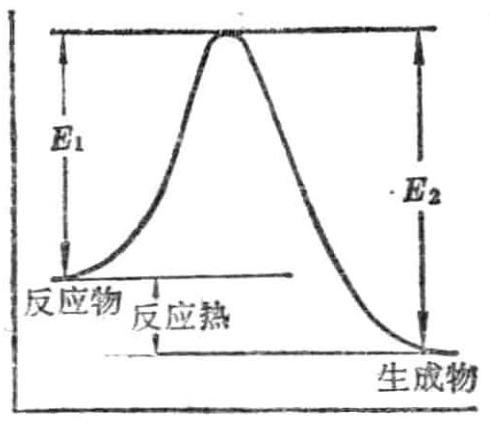
\includegraphics[max width=0.5\textwidth]{images/01912d13-9986-7822-a012-3f3f7be99dcb_70_696915.jpg}
\end{center}

图 3-2 反应过程中能量变化示意图

要吸收 \({E}_{1}\) 的能量,才能变成活化分子,这个能量 \({E}_{1}\) 就是该反应的活化能。活化分子变成生成物分子的过程中,要放出 \({E}_{2}\) 的能量。显然图中 \({E}_{2} > {E}_{1}\) ,在反应物变成生成物的整个过程中要放出 \({E}_{2} - {E}_{1}\) 的能量,这个能量就是反应热。图 3-2 所示的反应是放热反应。无论放热反应或吸热反应, 都需要有一个活化的过程。前面提到的在常温下煤在空气里必须加热才能燃烧, 就是因为加热能促使煤和氧气中的分子活化, 发生氧化反应, 反应发生后, 就可由放出的反应热维持反应继续进行, 而不需要外部再供给能量。

不同的化学反应所需的活化能不同。如果反应的活化能较低, 则在一定温度下, 活化分子百分数就较大, 反应就比较容易进行。

在其它条件不变时, 对某一反应来说, 反应物分子中活化分子的百分数是一定的, 因此, 单位体积内活化分子的数目与单位体积内反应物分子的总数成正比, 也就是和反应物的浓度成正比。当反应物浓度增大时, 单位体积内分子增多, 活化分子数也相应增大。譬如原来 1 单位体积里有 100 个反应物的分子, 其中只有 5 个活化分子, 如果每 1 单位体积内的反应物分子增加到 200 个, 其中必定有 10 个活化分子, 那么单位时间内的有效碰撞次数也相应增多, 反应就快。

在浓度一定时, 升高温度, 反应物的分子的能量增加, 必然有一部分原来能量较低的分子变成了活化分子, 从而增加了反应物分子中活化分子的百分数, 有效碰撞次数增多了, 因而加大了反应的速度。当然, 由于温度升高, 会使分子的运动加快, 这样单位时间内反应物分子间的碰撞次数增加, 反应也会相应地加快, 但这不是反应加快的主要原因。

\section*{4. 催化剂对反应速度的影响}

关于催化剂和催化作用的初步知识, 在氧气的实验室制法、硫酸的工业制法和氨的催化氧化等教材里都学习过了。现在我们要学习催化剂与化学反应速度的关系。

[实验 3-3] 在两个试管里分别加入 \(3\%\) 的过氧化氢 \(\left( {{\mathrm{H}}_{2}{\mathrm{O}}_{2}}\right)\) 溶液 3 毫升和合成洗涤剂 (产生泡沫以示有 气体生成) 溶液 3 或 4 滴。在其中的一个试管里加入少量 \({\mathrm{{MnO}}}_{2}\) ,观察两个试管里的反应现象有什么不同。

实验结果表明: 在放有少量 \({\mathrm{{MnO}}}_{2}\) 的试管中,很快有气泡生成,而没有放 \({\mathrm{{MnO}}}_{2}\) 的试管里气泡产生得慢而且少。这是由于 \({\mathrm{{MnO}}}_{2}\) 能加快 \({\mathrm{H}}_{2}{\mathrm{O}}_{2}\) 的分解; 使氧气产生得快而且多, 反应后 \({\mathrm{{MnO}}}_{2}\) 的组成和质量都没有变化。可见 \({\mathrm{{MnO}}}_{2}\) 在 \({\mathrm{H}}_{2}{\mathrm{O}}_{2}\) 的分解反应中起了催化作用。

\[
2{\mathrm{H}}_{2}{\mathrm{O}}_{2} = \frac{{\mathrm{{MnO}}}_{2}}{}2{\mathrm{H}}_{2}\mathrm{O} + {\mathrm{O}}_{2} \uparrow
\]

催化剂能够增大反应速度的原因, 是它能够降低反应的活化能, 从而使更多的反应物分子成为活化分子, 大大增加单位体积内反应物分子中活化分子的百分数, 成千成万倍地增大化学反应的速度。从图 3-3 可以清楚地看出催化剂与反应速度的关系。图中实线曲线表示不用催化剂时, 反应物变成生成物的过程, \({E}_{1}\) 是不用催化剂时的反应的活化能; 虚线曲线表示用催化剂时,反应物变成生成物的过程, \({E}_{2}\) 是有催化剂存在时该反应的活化能。显然, 使用催化剂能使反应的活化能降低, 因而能大大增大反应的速度。这好象人们要翻越一座陡峭的高山, 很费劲、很慢, 能翻越的人就少些; 如果在山下开凿一条隧道, 穿过隧道就容易、就快, 能穿过的人就多一样。

\begin{center}
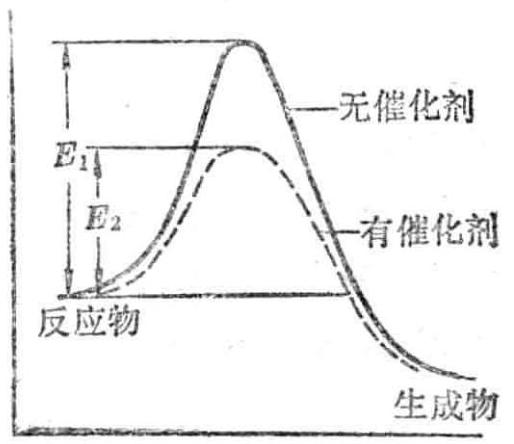
\includegraphics[max width=0.6\textwidth]{images/01912d13-9986-7822-a012-3f3f7be99dcb_72_684597.jpg}
\end{center}

图 3-3 催化剂与活化能的关系示意图

为什么使用适当的催化剂能够降低反应的活化能呢? 现以接触法制造硫酸使用的接触剂 \({\mathrm{V}}_{2}{\mathrm{O}}_{5}\) ,和合成氨工艺中使用的铁触媒为例, 来说明它们是怎样降低活化能的。

制造硫酸的过程中,关键是怎样把 \({\mathrm{{SO}}}_{2}\) 更快地转变为 \({\mathrm{{SO}}}_{3}\) 。如果使用 \({\mathrm{V}}_{2}{\mathrm{O}}_{5}\) 做催化剂时,有的化学工作者认为反应是按以下两步进行的:

\[
{\mathrm{{SO}}}_{2} + {\mathrm{V}}_{2}{\mathrm{O}}_{5} = {\mathrm{{SO}}}_{3} + {\mathrm{V}}_{2}{\mathrm{O}}_{4}
\]

\[
{V}_{2}{O}_{4} + {SO}_{2} + {O}_{2} = {SO}_{3} + {V}_{2}{O}_{5}
\]

可见使用 \({\mathrm{V}}_{2}{\mathrm{O}}_{5}\) 做催化剂,能使一步进行的反应 变成为分两步进行的反应。实验测得这样将会使反应活化能降低到原来的二分之一左右, 从而使反应速度大大加快。由此可见, 催化剂并不是不参与化学反应, 只是反应前与反应后的组成和质量未改变罢了。

在氢跟氮合成氨的过程中, 如果使用铁触媒时, 铁触媒能吸附氢分子和氮分子, 同时削弱氮分子和氢分子里的化学键, 化学键被削弱了的这两种分子互相碰撞而合成氨分子。由于使用铁触媒, 合成氨反应的活化能降低到原来的四分之一左右。同时由于吸附, 在铁触媒表面上反应物浓度增大了, 也能增大反应的速度。这样, 使用铁触媒的反应速度比无催化剂时成万倍地增大。

催化剂在现代化学和化工生产中占有极为重要的地位。 据初步统计约有 \({85}\%\) 的化学反应需要使用催化剂。尤其在当前大型化工生产、石油化学工业生产中, 很多反应还必须靠使用性能优良的催化剂来实现。但是应当注意, 因为有一些物质, 即使是很少量的, 当混入催化剂中时, 就会急剧降低甚至破坏催化剂的催化能力, 这种作用叫做催化剂的中毒。为了防止催化剂的中毒, 需要对原料进行一系列的净化过程。

影响化学反应速度的条件很多, 除了温度、浓度、压强 (有气体参加的反应)、催化剂以外, 还有光、超声波、激光、放射线、电磁波、反应物颗粒的大小、扩散速度、溶剂等等, 对某些化学反应来说, 也是影响反应速度的一些重要条件。例如, 煤粉的燃烧就比煤块快得多, 溴化银见光很快分解等等。

[讨论] 举出你学过或生活中接触过的实例, 说明影响反应速度的条件。

以上研究了影响反应速度的一些重要条件, 但在化学研究和化工生产中, 只考虑反应速度是不够的。例如, 在合成氨工业中除了要求氮和氢尽可能快地转变为氨外, 还要使氮和氢尽可能多地转变为氨。这就涉及到化学反应的另一个问题一化学平衡。下节就要研究关于化学平衡的问题。

\section*{习 题}

1. 举例说明加快和减慢反应速度的实际意义。

2. 在下列反应

\[
\mathrm{{CO}} + {\mathrm{H}}_{2}\mathrm{O} \rightleftharpoons {\mathrm{{CO}}}_{2} + {\mathrm{H}}_{2}
\]

里,起始浓度 \(\left\lbrack \mathrm{{CO}}\right\rbrack = \left\lbrack {{\mathrm{H}}_{2}\mathrm{O}}\right\rbrack = {0.02}\) 摩尔/升,1 分钟后测得 \(\left\lbrack \mathrm{{CO}}\right\rbrack = {0.005}\) 摩尔/升,求分别以 \(\mathrm{{CO}}\) 和 \({\mathrm{H}}_{2}\) 的浓度表示的反应速度。

3. 为什么反应的活化能低, 反应速度就较大呢?

4. 在空气中燃烧木炭是一个放热反应, 为什么木炭燃烧时必须先引火点燃? 点燃后停止加热, 能够继续燃烧吗? 为什么?

5. 在一块大理石 (主要成分是 \({\mathrm{{CaCO}}}_{3}\) ) 上,先后滴加 \({1M}\) \(\mathrm{{HCl}}\) 和 \({0.1M}\mathrm{{HCl}}\) ,哪个反应快? 先后滴加同浓度的热盐酸和冷盐酸, 哪个反应快? 用大理石块和大理石粉跟同浓度的盐酸起反应, 哪个反应快?

6. 在进行铁跟盐酸的反应时, 用什么方法可以使反应加快? 设计一个实验方法来粗略地衡量反应的速度。

7. 为什么升高温度和增加反应物的浓度, 都能增大反应的速度呢?

8. 为什么使用适当的催化剂能够使一些反应的速度增大呢?

9. 举例说明催化剂对化工生产的重要意义。

10. 为什么增加反应物分子中活化分子的百分数能够增大反应的速度呢? 用哪些方法可以增加反应物分子中活化分子的百分数呢?

\section*{第二节 化学平衡}

现在我们来学习化学平衡, 化学平衡主要是研究可逆反应的规律, 如反应进行的程度以及各种条件对反应进行情况的影响等等。

\section*{一、化学平衡是动态平衡}

固态溶质溶解在液态溶剂里, 当形成饱和溶液时, 达到溶解平衡。这时, 溶解的过程并没有停止, 只是溶解和结晶的速度相等罢了。因此, 溶解平衡是一种动态平衡。那么, 在化学反应中, 我们将要研究的可逆反应的情形又是怎样的呢? 我们可以通过下面的反应来进行研究。

\[
2{\mathrm{{SO}}}_{2} + {\mathrm{O}}_{2}\xrightarrow[\bigtriangleup ]{\text{ 催化剂 }}2{\mathrm{{SO}}}_{3}
\]

在 \({500}^{ \circ }\mathrm{C},1\) 标准大气压时,把 2 体积的二氧化硫和 1 体积的氧气的混和物, 通入一个装有催化剂的密闭容器里。反应开始后, \({\mathrm{{SO}}}_{2}\) 和 \({\mathrm{O}}_{2}\) 的浓度逐渐减小, \({\mathrm{{SO}}}_{3}\) 的浓度逐渐增大, 最后能得到含 \({91}\%\) (体积组成) 三氧化硫的混和气体。这时候,容器里反应物 \({\mathrm{{SO}}}_{2}\text{、}{\mathrm{O}}_{2}\) 和生成物 \({\mathrm{{SO}}}_{3}\) 在混和物中的浓度就不再发生变化。

为什么反应进行到一定程度, 生成物的含量就不继续增大了呢? 也就是说, 反应为什么不能进行到底呢? 我们可以用可逆反应中正反应和逆反应的反应速度的变化来说明。

当反应开始的时候, \({\mathrm{{SO}}}_{2}\) 和 \({\mathrm{O}}_{2}\) 的浓度最大,因而它们化合生成 \({\mathrm{{SO}}}_{3}\) 的正反应速度最大; 而 \({\mathrm{{SO}}}_{3}\) 的浓度为零,因而它分解生成 \({\mathrm{{SO}}}_{2}\) 和 \({\mathrm{O}}_{2}\) 的逆反应的速度也是零。以后,随着反应的进行,反应物 \({\mathrm{{SO}}}_{2}\) 和 \({\mathrm{O}}_{2}\) 的浓度逐渐减小,正反应的速度就逐渐减小; 生成物 \({\mathrm{{SO}}}_{3}\) 的浓度逐渐增大,逆反应的速度就逐渐增大。

如果外界条件不发生变化, 化学反应进行到一定程度的时候, 正反应和逆反应的速度相等, 反应物和生成物的浓度不再发生变化。这时反应物和生成物的混和物(简称反应混和物) 就处于化学平衡状态。

如果我们不是从 \({\mathrm{{SO}}}_{2}\) 和 \({\mathrm{O}}_{2}\) 的混和物开始反应,而是使纯净的 \({\mathrm{{SO}}}_{3}\) ,在同样的温度 \(\left( {{500}^{ \circ }\mathrm{C}}\right)\) 、压强 ( 1 标准大气压) 和催化剂存在的条件下起反应, \({\mathrm{{SO}}}_{3}\) 分解为 \({\mathrm{{SO}}}_{2}\) 和 \({\mathrm{O}}_{2}\) ,当达到平衡状态时,混和气体里仍然含 \({91}\%\) (体积)的 \({\mathrm{{SO}}}_{3}\) 。

当反应达到平衡的时候, 正反应和逆反应都仍在继续进行,只是由于在同一瞬间正反应 \({\mathrm{{SO}}}_{2}\) 和 \({\mathrm{O}}_{2}\) 化合生成的 \({\mathrm{{SO}}}_{3}\) 分子数和逆反应所分解的 \({\mathrm{{SO}}}_{3}\) 分子数相等,亦即正、逆反应的速度相等, 所以反应混和物中各成分的百分含量不变。因此, 化学平衡是一种动态平衡。

化学平衡状态就是指在一定条件下的可逆反应里, 正反应和逆反应的速度相等, 反应混和物中各组成成分的百分含量保持不变的状态。

\section*{二、化学平衡常数}

下面我们以一氧化碳和水蒸气在高温时进行反应生成二氧化碳和氢气为例, 来研究化学平衡的性质。

在密闭容器里这个反应不能进行到底, 而是达到了化学平衡状态。

\[
\mathrm{{CO}}\left( \text{ 气 }\right) + {\mathrm{H}}_{2}\mathrm{O}\text{ (气) }\underset{\text{ 高温 }}{\overset{\text{ 催化剂 }}{ \rightleftharpoons }}{\mathrm{{CO}}}_{2}\left( \text{ 气 }\right) + {\mathrm{H}}_{2}\text{ (气) }
\]

如果把 0.01 摩尔的 \(\mathrm{{CO}}\) 和 0.01 摩尔的 \({\mathrm{H}}_{2}\mathrm{O}\) (气) 放在 1 升的密闭容器里,加热到 \({800}^{ \circ }\mathrm{C}\) ,实验测得当生成物 \({\mathrm{{CO}}}_{2}\) 和 \({\mathrm{H}}_{2}\) 各为 0.005 摩尔时,反应即达到了平衡状态。达到了平衡的反应混和物 (简称平衡混和物) 里还有 0.005 摩尔的 \(\mathrm{{CO}}\) 和 0.005 摩尔的 \({\mathrm{H}}_{2}\mathrm{O}\) (气)。这可以表示如下:

\[
\mathrm{{CO}} + {\mathrm{H}}_{2}\mathrm{O}\left( \text{ 气 }\right) \mathop{\rightleftharpoons }\limits^{{{800}^{ \circ }\mathrm{C}}}{\mathrm{{CO}}}_{2} + {\mathrm{H}}_{2}
\]

反应开始时,

各物质的摩尔数 \(\;{0.01}\;{0.01}\;0\)

达到平衡时,

各物质的摩尔数 \(\;{0.0050.005}\;{0.005}\;{0.005}\)

由于密闭容器的容积是 1 升, 因此各物质的摩尔数在数值上跟它们的摩尔浓度 (以摩尔/升为单位) 相同。如果我们用符号 \(\left\lbrack \right\rbrack\) 表示某物质的浓度,那么上面的例子也可以写成:

\(\left\lbrack \mathrm{{CO}}\right\rbrack \;\left\lbrack {{\mathrm{H}}_{2}\mathrm{O}}\right\rbrack \;\left\lbrack {\mathrm{{CO}}}_{2}\right\rbrack \;\left\lbrack {\mathrm{H}}_{2}\right\rbrack\)

反应开始时, 各物质的

浓度(摩尔/升) 0.01 0.01 0 0

达到平衡时, 各物质的

浓度(摩尔/升) 0.005 0.005 0.005 0.005

为了进一步了解可逆反应达到化学 平衡 状态时的特点, 对于上述反应, 可以进行以下的实验。设在四个 1 升的密闭容器里,分别在每个容器里通入不同摩尔数的 \(\mathrm{{CO}}\text{、}{\mathrm{H}}_{2}\mathrm{O}\left( \text{气}\right) \text{、}{\mathrm{{CO}}}_{2}\) 和 \({\mathrm{H}}_{2}\) ,如表 3-1 中起始浓度一栏所表示的那样。把四个密闭容器加热到 \({800}^{ \circ }\mathrm{C}\) ,经过足够的时间以后,如果这四个容器里的四种物质的浓度并不再随时间的改变而改变, 那么, 这四个容器里的反应混和物就都达到了平衡状态。把实验测得的平衡浓度的数据列在表 3-1 的第二栏里。为了研究在平衡混和物中各物质浓度之间的关系, 我们用平衡混和物中各生成物的浓度乘积作为分子, 把各反应物的浓度乘积作为分母, 求其比值。并把求得的数值列入表 3-1 的第三栏里。

表 3-1 \(\mathrm{{CO}} + {\mathrm{H}}_{2}\mathrm{O}\) (气) \(\rightleftharpoons {\mathrm{{CO}}}_{2} + {\mathrm{H}}_{2}\) 反应中

起始和平衡时各物质的浓度 \(\left( {{800}^{ \circ }\mathrm{C}}\right)\)

\begin{center}
\adjustbox{max width=\textwidth}{
\begin{tabular}{|c|c|c|c|c|c|c|c|c|}
\hline
\multicolumn{4}{|c|}{起始时 各物质的浓度 (摩尔/升)} & \multicolumn{4}{|c|}{平衡时 各物质的浓度 (摩尔/升)} & 平衡时 \(\left\lbrack {\mathrm{{CO}}}_{2}\right\rbrack \left\lbrack {\mathrm{H}}_{2}\right\rbrack\) \\
\hline
[CO] & \(\left\lbrack {{\mathrm{H}}_{2}\mathrm{O}}\right\rbrack\) & [CO \({}_{2}\) ] & \(\left\lbrack {\mathrm{H}}_{2}\right\rbrack\) & [CO] & \(\left\lbrack {{\mathrm{H}}_{2}\mathrm{O}}\right\rbrack\) & [CO \({}_{2}\) ] & \(\left\lbrack {\mathrm{H}}_{2}\right\rbrack\) & [CO][H \({}_{2}\) O] \\
\hline
0.01 & 0.01 & 0 & 0 & 0.005 & 0.005 & 0.005 & 0.005 & 1.0 \\
\hline
0 & 0 & 0.02 & 0.01 & 0.0067 & 0.0067 & 0.0133 & 0.0033 & 1.0 \\
\hline
0.0025 & 0.03 & 0.0075 & 0.0075 & 0.0021 & 0.0296 & 0.0079 & 0.0079 & 1.0 \\
\hline
0.01 & 0.03 & 0 & 0 & 0.0025 & 0.0225 & 0.0075 & 0.0075 & 1.0 \\
\hline
\end{tabular}
}
\end{center}

从上表所列出的实验数据, 可以得出如下的结论:

在一定温度下, 可逆反应无论从正反应开始, 或是从逆反应开始, 又无论反应起始时反应物浓度的大小, 最后都能达到平衡。这时生成物的浓度乘积除以反应物的浓度乘积, 便得到一个比值, 而这个比值是个常数, 这个常数叫做该反应的化学平衡常数 (简称平衡常数)。用符号 \(K\) 表示。例如,在 \({800}^{ \circ }\mathrm{C}\) 时,

\(\frac{\left\lbrack {\mathrm{{CO}}}_{2}\right\rbrack \left\lbrack {\mathrm{H}}_{2}\right\rbrack }{\left\lbrack \mathrm{{CO}}\right\rbrack \left\lbrack {{\mathrm{H}}_{2}\mathrm{O}}\right\rbrack } = 1\) 。化学平衡常数 \(K\) 的数值为 1 。

为了更好地认识化学平衡状态的性质, 下面我们还可以再研究一个可逆反应的例子。

\[
{\mathrm{H}}_{2} + {\mathrm{I}}_{2}\left( \text{ 气 }\right) \rightleftharpoons 2\mathrm{{HI}}
\]

在三个 1 升的密闭容器里, 分别在其中通入不同摩尔数的 \({\mathrm{H}}_{2}\text{、}{\mathrm{I}}_{2}\) 或 \(\mathrm{{HI}}\) ,如表 3-2 中起始浓度一栏所示。把三个密闭容器都加热到 \({445}^{ \circ }\mathrm{C}\) ,经过足够的时间,使它们都达到平衡状态。把实验测得的平衡状态时各物质的浓度数 据列在表 3-2 的第二栏里。然后,我们用平衡混和物中各生成物浓度与反应物浓度计算其不同的比值, 并把求得的数值列入表 3-2 的第三栏和第四栏里。

表 \(3 - 2{\mathrm{H}}_{2} + {\mathrm{I}}_{2}\left( \text{气}\right) \rightleftharpoons 2\mathrm{{HI}}\) 反应中起始和平衡时各物质的浓度 \(\left( {{445}^{ \circ }\mathrm{C}}\right)\)

\begin{center}
\adjustbox{max width=\textwidth}{
\begin{tabular}{|c|c|c|c|c|c|c|c|}
\hline
\multicolumn{3}{|c|}{起始时 各物质的浓度 (摩尔/升)} & \multicolumn{3}{|c|}{平衡时 各物质的浓度 (摩尔/升)} & 平衡时 [HI] & \multirow{2}{*}{平衡时 [HI]2 \(\left\lbrack {\mathrm{H}}_{2}\right\rbrack \left\lbrack {\mathrm{I}}_{2}\right\rbrack\)} \\
\cline{1-7}
[H.] & \(\left\lbrack {\mathrm{I}}_{2}\right\rbrack\) & [HI] & \(\left\lbrack {\mathrm{H}}_{2}\right\rbrack\) & \(\left\lbrack {\mathrm{I}}_{2}\right\rbrack\) & [HI] & \(\left\lbrack {\mathrm{H}}_{2}\right\rbrack \left\lbrack {\mathrm{I}}_{2}\right\rbrack\) & \\
\hline
0.01 & 0.01 & 0 & 0.0022 & 0.0022 & 0.0156 & 3223 & 50 \\
\hline
0 & 0 & 0.01 & 0.0011 & 0.0011 & 0.0078 & 6446 & 50 \\
\hline
0 & 0.0097 & 0.0349 & 0.0017 & 0.0114 & 0.0315 & 1625 & 51 \\
\hline
\end{tabular}
}
\end{center}

从上表所列出的数据可以看出, 如果用平衡时反应物的浓度乘积去除生成物的浓度, 如下式:

\begin{center}
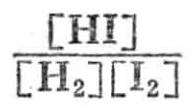
\includegraphics[max width=0.2\textwidth]{images/01912d13-9986-7822-a012-3f3f7be99dcb_80_469735.jpg}
\end{center}

其比值就不是一个常数。但是如用反应物浓度的乘积 \(\left\lbrack {\mathrm{H}}_{2}\right\rbrack \left\lbrack {\mathrm{I}}_{2}\right\rbrack\) .

去除生成物浓度的平方[HI] \({}^{2}\) ,即

\[
\frac{{\left\lbrack \mathrm{{HI}}\right\rbrack }^{2}}{\left\lbrack {\mathrm{H}}_{2}\right\rbrack \left\lbrack {\mathrm{I}}_{2}\right\rbrack }
\]

我们发现在表里所列三种不同的情况下, 仍然可以得到一个比例常数,即 \(K = {50}\) 。这个常数就是这个反应在 \({445}^{ \circ }\mathrm{C}\) 时的化学平衡常数。

对于一般的可逆反应

\[
m\mathrm{\;A} + n\mathrm{\;B} \rightleftharpoons p\mathrm{C} + q\mathrm{D}
\]

其中 \(\mathbf{A}\text{、}\mathbf{B}\) 代表反应物, \(\mathbf{C}\text{、}\mathbf{D}\) 代表生成物, \(m\text{、}n\text{、}p\text{、}q\) 分别表示化学方程式中各反应物和生成物的分子式前的系数。当在一定温度下达到平衡时, 可以写出:

\[
\frac{{\left\lbrack \mathrm{C}\right\rbrack }^{p}{\left\lbrack \mathrm{D}\right\rbrack }^{q}}{{\left\lbrack \mathrm{\;A}\right\rbrack }^{m}{\left\lbrack \mathrm{\;B}\right\rbrack }^{n}} = K
\]

\(K\) 就叫做这个反应的平衡常数。

在平衡常数的表达式中, 通常把生成物的浓度写在分式分子的位置, 反应物的浓度写在分母的位置; 式中每种物质浓度的方次数就是化学方程式中该物质分子式前的系数。

从平衡常数 \(K\) 值的大小,可以推断反应进行的程度。 \(K\) 值越大, 表示化学反应达到平衡时生成物浓度对反应物浓度的比值越大,也就是反应进行得更完全些,反应物的转化率 \(\Phi\) 也越大。反之, \(K\) 值越小,表示反应进行的程度越小,反应物的转化率也越小。

通过前面学习过的实验事实, 我们知道在一定温度时, 一个可逆反应的平衡常数并不随反应物或生成物浓度的改变而改变。但当温度改变时,情形就不同了,平衡常数 \(K\) 值随温度的改变而改变。

例如, 氢气跟碘化合生成碘化氢的反应:

① 某个指定反应物的转化率

\(= \frac{\text{ 指定反应物的起始浓度 } - \text{ 指定反应物的平衡浓度 }}{\text{ 指定反应物的起始浓度 }} \times {100}\%\)

\[
{\mathrm{H}}_{2}\left( \text{ 气 }\right) + {\mathrm{I}}_{2}\left( \text{ 气 }\right) \rightleftharpoons 2\mathrm{{HI}}\left( \text{ 气 }\right)
\]

在不同温度时, 其平衡常数不同, 数值分别是:

\({350}^{ \circ }\mathrm{C},K = {66.9}_{;}{425}^{ \circ }\mathrm{C},K = {54.4}_{;}{490}^{ \circ }\mathrm{C},K = {45.9}_{ \circ }\)

因此, 在使用平衡常数时, 必须注意是在哪一温度下进行的可逆反应。

[例题1] 把 0.01 摩尔的 \({\mathrm{{CO}}}_{2}{}^{r}\) 和 0.01 摩尔的 \({\mathrm{H}}_{2}\) 放在 1 升的密闭容器里,加热到 \({1200}^{ \circ }\mathrm{C}\) ,在生成 0.006 摩尔的 \(\mathrm{{CO}}\) 和 0.006 摩尔的 \({\mathrm{H}}_{2}\mathrm{O}\) (气) 的时候,反应达到平衡。试求这时该反应的化学平衡常数。

[解] \({\mathrm{H}}_{2} \rightleftharpoons \mathrm{{CO}} + {\mathrm{H}}_{2}\mathrm{O}\) (气)

反应开始时各 0.01 0.01 0

物质的摩尔数

达到平衡时各 \({0.01} - {0.006}\;{0.01} - {0.006}\;{0.006}\;{0.006}\) 物质的摩尔数

因在 1 升的容器里, 所以, 平衡时各参加反应物质的浓度分别是:

\(\left\lbrack \mathrm{{CO}}\right\rbrack = {0.006}\) 摩尔/升, \(\left\lbrack {{\mathrm{H}}_{2}\mathrm{O}}\right\rbrack = {0.006}\) 摩尔/升,

\(\left\lbrack {\mathrm{{CO}}}_{2}\right\rbrack = {0.004}\) 摩尔/升, \(\left\lbrack {\mathrm{H}}_{2}\right\rbrack = {0.004}\) 摩尔/升,

\[
K = \frac{\left\lbrack \mathrm{{CO}}\right\rbrack \left\lbrack {{\mathrm{H}}_{2}\mathrm{O}}\right\rbrack }{\left\lbrack {\mathrm{{CO}}}_{2}\right\rbrack \left\lbrack {\mathrm{H}}_{2}\right\rbrack } = \frac{{0.006} \times {0.006}}{{0.004} \times {0.004}} = {2.25}
\]

答: 在 \({1200}^{ \circ }\mathrm{C}\) 时,这个反应的平衡常数是 2.25 。

[例题2] 设在某温度时, 在容积为 1 升的密闭容器里, 把 \({\mathrm{N}}_{2}\) 和 \({\mathrm{H}}_{2}\) 两种气体混和,反应后生成 \({\mathrm{{NH}}}_{3}\) 。从实验测得, 当达到平衡时, \({\mathrm{N}}_{2}\) 和 \({\mathrm{H}}_{2}\) 的浓度各为 2 摩尔/升,生成的 \({\mathrm{{NH}}}_{3}\) 的浓度是 3 摩尔/升,求这个反应在某温度的平衡常数和 \({\mathrm{N}}_{2}\) 、 \({\mathrm{H}}_{2}\) 两气体在反应开始时的浓度。

[解]

\[
{\mathrm{N}}_{2} + 3{\mathrm{H}}_{2} \rightleftharpoons 2{\mathrm{{NH}}}_{3}
\]

在某温度时,平衡混和物中 \({\mathrm{N}}_{2}\text{、}{\mathrm{H}}_{2}\) 和 \({\mathrm{{NH}}}_{3}\) 的浓度分别是: \(\left\lbrack {\mathrm{N}}_{2}\right\rbrack = 2\) 摩尔/升, \(\left\lbrack {\mathrm{H}}_{2}\right\rbrack = 2\) 摩尔/升, \(\left\lbrack {\mathrm{{NH}}}_{3}\right\rbrack = 3\) 摩尔/升。

\[
K = \frac{{\left\lbrack {\mathrm{{NH}}}_{3}\right\rbrack }^{2}}{\left\lbrack {\mathrm{\;N}}_{2}\right\rbrack {\left\lbrack {\mathrm{H}}_{2}\right\rbrack }^{3}} = \frac{{3}^{2}}{2 \times {2}^{3}} = \frac{9}{16} = {0.563}
\]

由化学方程式可以知道,生成 3 摩尔 \({\mathrm{{NH}}}_{3}\) ,必须消耗 1.5 摩尔的 \({\mathrm{N}}_{2}\) 和 4.5 摩尔的 \({\mathrm{H}}_{2},{\mathrm{\;N}}_{2}\) 和 \({\mathrm{H}}_{2}\) 在反应开始时的浓度应是消耗量和在平衡时剩余量之和。所以,

\({\mathrm{N}}_{2}\) 在反应开始时的浓度 \(= {1.5} + 2 = {3.5}\) 摩尔/升

\({\mathrm{H}}_{2}\) 在反应开始时的浓度 \(= {4.5} + 2 = {6.5}\) 摩尔/升

答: 这个反应在某温度的平衡常数是 \({0.563},{\mathrm{\;N}}_{2}\) 在反应开始时的浓度为 3.5 摩尔/升, \({\mathrm{H}}_{2}\) 在反应开始时的浓度为 6.5 摩尔/升。

〔例题 3 】在密闭容器中, 给一氧化碳和水蒸气混和物加热时, 达到下列平衡:

\[
\mathrm{{CO}} + {\mathrm{H}}_{2}\mathrm{O}\left( \text{ 气 }\right) \rightleftharpoons {\mathrm{{CO}}}_{2} + {\mathrm{H}}_{2}
\]

在 \({800}^{ \circ }\mathrm{C}\) 时平衡常数等于 1,若用 2 摩尔的 \(\mathrm{{CO}}\) 和 10 摩尔的 \({\mathrm{H}}_{2}\mathrm{O}\) 互相混和并加热到 \({800}^{ \circ }\mathrm{C}\) ,求 \(\mathrm{{CO}}\) 转化为 \({\mathrm{{CO}}}_{2}\) 的转化率?

由于平衡常数表达式中各物质的浓度都是平衡时的浓度, 因此在利用平衡常数的计算中, 都必须首先列出平衡时各物质的浓度。

[解] 设 \(x =\) 达到平衡时 \(\mathrm{{CO}}\) 转化为 \({\mathrm{{CO}}}_{2}\) 的摩尔数

\(V =\) 容器的容积

\(\mathrm{{CO}} + {\mathrm{H}}_{2}\mathrm{O}\left( \text{ 气 }\right) \rightleftharpoons {\mathrm{{CO}}}_{2} + {\mathrm{H}}_{2}\)

反应开始时的浓度 \(\frac{2}{V}\;\frac{10}{V}\;\frac{0}{V}\;\frac{0}{V}\)

达到平衡时的浓度 \(\frac{2 - x}{V}\;\frac{{10} - x}{V}\;\frac{x}{V}\;\frac{x}{V}\)

将平衡浓度代入平衡常数表达式, 则得:

\[
K = \frac{\left\lbrack {\mathrm{{CO}}}_{2}\right\rbrack \left\lbrack {\mathrm{H}}_{2}\right\rbrack }{\left\lbrack \mathrm{{CO}}\right\rbrack \left\lbrack {{\mathrm{H}}_{2}\mathrm{O}}\right\rbrack } = \frac{\frac{{x}^{2}}{{V}^{2}}}{\frac{2 - x}{V} \cdot \frac{{10} - x}{V}} = 1
\]

\[
{x}^{2} = \left( {2 - x}\right) \left( {{10} - x}\right)
\]

\[
{x}^{2} = {20} - {12x} + {x}^{2}
\]

\[
x = \frac{20}{12} = {1.66}
\]

\(\mathrm{{CO}}\) 转化为 \({\mathrm{{CO}}}_{2}\) 的百分率为:

\[
\frac{1.66}{2} \times {100}\% = {83}\%
\]

答: \(\mathrm{{CO}}\) 转化为 \({\mathrm{{CO}}}_{2}\) 的转化率是 \({83}\%\) 。

\section*{习 题}

1. 已知 \({\mathrm{{PCl}}}_{5}\left( \text{气}\right) \rightleftharpoons {\mathrm{{PCl}}}_{3}\left( \text{气}\right) + {\mathrm{{Cl}}}_{2}\left( \text{气}\right)\)

在 \({230}^{ \circ }\mathrm{C}\) 达到平衡时,平衡混和物中各物质的浓度分别是 \(\left\lbrack {\mathrm{{PCl}}}_{5}\right\rbrack = {0.47}\) 摩尔/升, \(\left\lbrack {\mathrm{{PCl}}}_{3}\right\rbrack = {0.098}\) 摩尔/升, \(\left\lbrack {\mathrm{{Cl}}}_{2}\right\rbrack =\) 0.098 摩尔/升, 求这个反应的平衡常数。

2. 已知 \({\mathrm{H}}_{2}\) (气) \(+ {\mathrm{I}}_{2}\) (气) \(\rightleftharpoons 2\mathrm{{HI}}\) (气)

在 \({445}^{ \circ }\mathrm{C}\) 时,平衡常数 \(K = {50}\) 。计算在 \({445}^{ \circ }\mathrm{C}\) 时,下面反应的平衡常数。

\[
2\mathrm{{HI}}\left( \text{ 气 }\right) \rightleftharpoons {\mathrm{H}}_{2}\left( \text{ 气 }\right) + {\mathrm{I}}_{2}\left( \text{ 气 }\right)
\]

3. 在 \({25}^{ \circ }\mathrm{C}\) 时, \({\mathrm{{NO}}}_{2}\) 与 \({\mathrm{N}}_{2}{\mathrm{O}}_{4}\) 处于平衡状态,两种气体的平衡混和物中含有 0.0125 摩尔/升的 \({\mathrm{{NO}}}_{2}\) 和 0.0321 摩尔/升的 \({\mathrm{N}}_{2}{\mathrm{O}}_{4}\) 。求这个反应的平衡常数。

4. 在一定温度时,2 摩尔 \({\mathrm{{COCl}}}_{2}\) 在 1 升的密闭容器里 - 分解,达到平衡时,测得已有 \({50}\%\) 的 \({\mathrm{{COCl}}}_{2}\) 分解成 \(\mathrm{{CO}}\) 和 \({\mathrm{{Cl}}}_{2}\) 。

\[
{\mathrm{{COCl}}}_{2}\left( \text{ 气 }\right) \rightleftharpoons \mathrm{{CO}}\left( \text{ 气 }\right) + {\mathrm{{Cl}}}_{2}\left( \text{ 气 }\right)
\]

求在此温度时, 这一反应的平衡常数。

*5. 在 1 升的密闭容器里,装有 3 摩尔的 \({\mathrm{{NO}}}_{2}\) ,在一定温度时进行下面的反应: \(2{\mathrm{{NO}}}_{2}\) (气) \(\rightleftharpoons {\mathrm{N}}_{2}{\mathrm{O}}_{4}\) (气),反应的平衡常数 \(K = {7.15}\) ,求在平衡时,该容器中的 \({\mathrm{{NO}}}_{2}\) 的摩尔数。

*6. 在密闭容器中将 \({\mathrm{{NO}}}_{2}\) 加热到某温度时,进行如下的反应:

\[
2{\mathrm{{NO}}}_{2} \rightleftharpoons 2\mathrm{{NO}} + {\mathrm{O}}_{2}
\]

在平衡时各物质的浓度是: \(\left\lbrack {\mathrm{{NO}}}_{2}\right\rbrack = {0.06}\) 摩尔/升, \(\left\lbrack \mathrm{{NO}}\right\rbrack =\) 0.24 摩尔/升, \(\left\lbrack {\mathrm{O}}_{2}\right\rbrack = {0.12}\) 摩尔/升。试求这温度下的平衡常数和 \({\mathrm{{NO}}}_{2}\) 在反应开始时的浓度。

*7. 已知一氧化碳跟水蒸气的反应为:

\[
\mathrm{{CO}} + {\mathrm{H}}_{2}\mathrm{O}\text{ (气) } \rightleftharpoons {\mathrm{{CO}}}_{2} + {\mathrm{H}}_{2}
\]

在 \({427}^{ \circ }\mathrm{C}\) 时的平衡常数为 9.4,若反应开始时,一氧化碳和水蒸气的浓度都是 0.01 摩尔/升, 试计算在此反应条件下一氧化碳的转化率。

\section*{第三节 影响化学平衡的条件}

化学平衡状态只有在一定的条件下才能保持。如果一个可逆反应达到平衡状态以后, 反应条件 (如浓度、压强、温度等) 改变了, 平衡混和物里各组成物质的百分含量也就随着改变而达到新的平衡状态, 这叫做化学平衡的移动。

下面着重讨论浓度、压强和温度的改变对化学平衡的影响。

\section*{一、浓度对化学平衡的影响}

当一个化学反应达到平衡的时候, 其它反应条件不变, 只改变其中任何一种反应物或生成物的浓度, 就会改变正反应或逆反应的反应速度, 使它们不再相等, 从而使平衡移动。

[实验 3-4] 在一个小烧杯里混和 10 毫升 \({0.01}\mathrm{M}\) 氯化铁溶液和 10 毫升 \({0.01}\mathrm{M}\) 硫氰化钾溶液,溶液立即变成红色。

把这红色溶液平均分到三个试管里, 在第一个试管里加入少量 \({1M}\) 氯化铁溶液,在第二个试管里加入少量 \({1M}\) 硫氰化钾溶液。观察这两个试管里溶液颜色的变化, 并跟第三个试管相比较。

氯化铁跟硫氰化钾(KSCN)起反应, 生成红色的硫氰化铁 \(\mathrm{{Fe}}{\left( \mathrm{{SCN}}\right) }_{3}\) ①和氯化钾,这个反应可表示如下:

\[
{\mathrm{{FeCl}}}_{3} + 3\mathrm{{KSCN}} \rightleftharpoons \mathrm{{Fe}}{\left( \mathrm{{SCN}}\right) }_{3} + 3\mathrm{{KCl}}
\]

(红色)

\customfootnote{

① 实际上主要是 \({\mathrm{{FeSCN}}}^{2 + }\) 离子的颜色。

}

从上面实验可知, 在平衡混和物里, 当加入氯化铁溶液或硫氰化钾溶液以后,溶液的颜色都变深了。这说明增大了任何一种反应物的浓度都促使化学平衡向正反应的方向移动, 生成更多的硫氰化铁。

其它实验也可证明, 在达到平衡的反应里, 减小任何一种生成物的浓度, 平衡会向正反应的方向移动; 减小任何一种反应物的浓度, 平衡会向逆反应的方向移动。

由此可见, 在其它条件不变的情况下, 增大反应物的浓度, 或减小生成物的浓度, 都可以使平衡向着正反应的方向移动; 增大生成物的浓度或减小反应物的浓度, 都可以使平衡向着逆反应的方向移动。

在生产上, 往往采用增大容易取得的或成本较低的反应物浓度的方法, 使成本较高的原料得到充分利用。例如, 在硫酸工业里, 常用过量的空气使二氧化硫被充分氧化。

\section*{二、压强对化学平衡的影响}

处于平衡状态的反应混和物里, 不管是反应物或生成物, 只要有气态物质存在, 那么改变压强也常常会使化学平衡移动。

[实验 3-5] 如图 3-4, 用注射器 (50 毫升或更大些的) 吸入约 20 毫升二氧化氮和四氧化二氮的混和气体 (使注射器的活塞达到 I 处)。吸入气体后, 将细管端用橡皮塞加以封闭。然后把注射器的活塞往外拉到 II 处。观察当活塞反复地从 II 到 I 及从 I 到 II 时, 管内混和气体颜色的变化。

\begin{center}
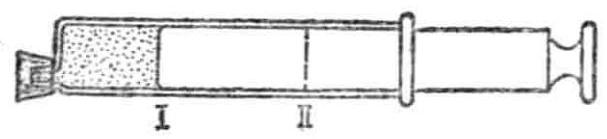
\includegraphics[max width=0.7\textwidth]{images/01912d13-9986-7822-a012-3f3f7be99dcb_87_801474.jpg}
\end{center}

图 3-4 压强对化学平衡的影响

二氧化氮(棕色气体)跟四氧化二氮(无色气体)在一定条件下处于化学平衡状态。在这个反应里,每减少二体积的 \({\mathrm{{NO}}}_{2}\) , 就会生成一体积的 \({\mathrm{N}}_{2}{\mathrm{O}}_{4}\) 。

\[
2{\mathrm{{NO}}}_{2}\left( \text{ 气 }\right) \rightleftharpoons {\mathrm{N}}_{2}{\mathrm{O}}_{4}\left( \text{ 气 }\right)
\]

\[
\text{( 2 体积, 棕色) ( 1 体积, 无色)}
\]

从实验 3-5 中可知, 把注射器的活塞往外拉, 管内体积增大, 气体的压强减小, 浓度减小, 混和气体的颜色先变浅又逐渐变深。逐渐变深是因为平衡向逆反应的方向移动, 生成了更多的 \({\mathrm{{NO}}}_{2}\) 。把注射器的活塞往里压,管内体积减小,气体的压强增大, 浓度增大, 混和气体的颜色先变深又逐渐变浅。 逐渐变浅是因为平衡向正反应的方向移动,生成了更多的 \({\mathrm{N}}_{2}{\mathrm{O}}_{4}\) 。

从上面的实验可以看出, 在其它条件不变的情况下, 增大压强会使化学平衡向着气体体积缩小的方向移动; 减小压强, 会使平衡向着气体体积增大的方向移动。

在有些可逆反应里, 反应前后气态物质的总体积没有变化, 例如:

\[
2\mathrm{{HI}} \rightleftharpoons {\mathrm{H}}_{2} + {\mathrm{I}}_{2}\text{ (气) }
\]

\[
\text{( 2 体积) ( 1 体积) ( 1 体积)}
\]

在这种情况下, 增大或减小压强就不能使化学平衡移动。

固态物质或液态物质的体积, 受压强的影响很小, 可以略去不计。因此, 平衡混和物都是固体或液体的, 改变压强不能使平衡移动。

\section*{三、温度对化学平衡的影响}

在吸热或放热的可逆反应里, 反应混和物达到平衡状态以后, 改变温度也会使化学平衡移动。

[实验 3-6] 装置如图 3-5 所示, 两个连通着的烧瓶里, 盛有二氧化氮跟四氧化二氮达到平衡的混和气体。然后用夹子夹住橡皮管把一个烧瓶放进热水里, 把另一个烧瓶放入冰水 (或冷水) 里, 观察混和气体的颜色的变化。

\begin{center}
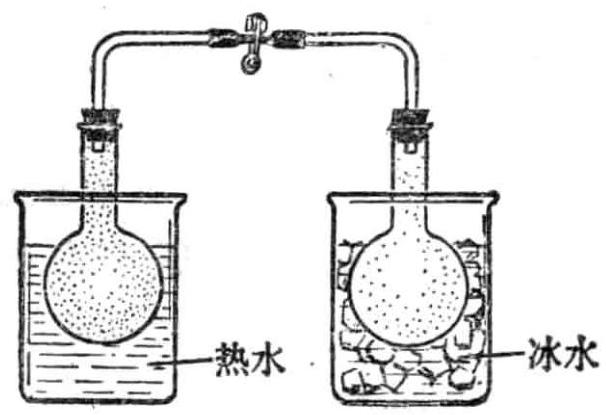
\includegraphics[max width=0.7\textwidth]{images/01912d13-9986-7822-a012-3f3f7be99dcb_89_910989.jpg}
\end{center}

图 3-5 温度对化学平衡的影响

在二氧化氮生成四氧化二氮的反应里, 正反应是放热反应, 逆反应是吸热反应。

\[
2{\mathrm{{NO}}}_{2} \rightleftharpoons {\mathrm{N}}_{2}{\mathrm{O}}_{4} + {13.6}\text{千卡}
\]

从上面实验可以知道, 混和气体受热颜色变深, 说明二氧化氮浓度增大, 平衡向逆反应方向移动。混和气体被冷却, 颜色变浅, 说明二氧化氮浓度减小, 平衡向正反应的方向移动。

由此可见, 在其他条件不变的情况下, 温度升高, 会使化学平衡向着吸热反应的方向移动; 温度降低, 会使化学平衡向着放热反应的方向移动。

浓度、压强、温度对化学平衡的影响可以概括成一个原理来表示, 这就是勒沙特列 \({}^{\left( 1\right) }\) 原理 (亦称平衡移动原理): 如果改变影响平衡的一个条件 (如浓度、压强或温度等), 平衡就向能够减弱这种改变的方向移动。

由于催化剂能够同样地增加正反应和逆反应的速度, 因此它对化学平衡的移动没有影响, 也就是说它不能改变达到化学平衡状态的反应混和物的百分组成。但是使用了催化剂, 就能够大大地缩短反应达到平衡所需的时间。

\section*{习 题}

1. 下述反应达到平衡时,

\[
2\mathrm{{NO}} + {\mathrm{O}}_{2} \rightleftharpoons 2{\mathrm{{NO}}}_{2} + {27.02}\text{ 千卡 }
\]

如果 (1) 增大压强,(2) 增大 \({\mathrm{O}}_{2}\) 的浓度,(3) 减小 \({\mathrm{{NO}}}_{2}\) 的浓度, (4) 升高温度, 平衡将向什么方向移动? 并简述理由。

2. 指出怎样改变反应物的浓度, 可使下列反应的平衡向正反应方向移动? ( \(\mathrm{C}\) 的浓度不变化)

\[
{\mathrm{{CO}}}_{2} + \mathrm{C}\left( \text{ 固 }\right) \rightleftharpoons 2\mathrm{{CO}}
\]

如果升高温度, 可使平衡向正反应方向移动, 那么, 生成一氧化碳的反应是放热反应还是吸热反应?

3. 增大压强和升高温度对下面处于平衡状态的化学反应有什么影响? 并说明原因。

(1) \(2\mathrm{{NO}} + {\mathrm{O}}_{2} \rightleftharpoons 2{\mathrm{{NO}}}_{2} + {27.02}\) 千卡

(2) \({\mathrm{N}}_{2} + {\mathrm{O}}_{2} \rightleftharpoons 2\mathrm{{NO}} - {43.2}\) 千卡

4. 化学反应

\(\mathrm{{CO}}\left( \text{ 气 }\right) + {\mathrm{{NO}}}_{2}\left( \text{ 气 }\right) \rightleftharpoons {\mathrm{{CO}}}_{2}\left( \text{ 气 }\right) + \mathrm{{NO}}\left( \text{ 气 }\right) + {54.1}\) 千卡在达到平衡时, 如果 (1) 升高温度, (2) 容器容积扩大到十倍, 平衡将分别受到什么影响?

\customfootnote{

① 勒沙特列(H. L. Le Chatelier, 1850-1936), 法国化学家。

}

5. 在下面反应中, 升高温度或降低温度对平衡有何影响?

\[
{\mathrm{H}}_{2}\mathrm{\;S} \rightleftharpoons {\mathrm{H}}_{2} + \mathrm{S}\text{ (固) } - 5\text{ 千卡 }
\]

6. 在密闭容器里, 对一氧化碳和水蒸气的混和物加热时, 达到下列平衡:

\[
\mathrm{{CO}} + {\mathrm{H}}_{2}\mathrm{O}\left( \text{ 气 }\right) \rightleftharpoons {\mathrm{{CO}}}_{2} + {\mathrm{H}}_{2}
\]

在 \({500}^{ \circ }\mathrm{C}\) 时平衡常数 \(K = 9\) ,如果反应开始时, \(\mathrm{{CO}}\) 反 \({\mathrm{H}}_{2}\mathrm{O}\) (气) 的浓度都是 0.02 摩尔/升,求 \(\mathrm{{CO}}\) 转化为 \({\mathrm{{CO}}}_{2}\) 的百分率?

7. 在某温度下,当 \({\mathrm{H}}_{2} + {\mathrm{{Br}}}_{2}\) (气) \(\rightleftharpoons 2\mathrm{{HBr}}\) 的反应达到平衡时, 各反应物质的浓度分别是:

\[
\left\lbrack {\mathrm{H}}_{2}\right\rbrack = {0.5}\text{摩尔}/\text{升,}
\]

\[
\left\lbrack {\mathrm{{Br}}}_{2}\right\rbrack = {0.1}\text{摩尔/升,}
\]

\[
\left\lbrack \mathrm{{HBr}}\right\rbrack = {1.6}\text{摩尔/升。}
\]

求氢气和溴(气)的起始浓度和平衡常数。

\section*{第四节 合成氨工业}

在这一节里, 我们将讨论怎样应用学过的化学反应速度和化学平衡的知识来研究有关合成氨的一些问题。

一、应用化学反应速度和化学平衡原理, 选择合成氨的适宜条件。

氨的合成是一个放热的、气体总体积缩小的可逆反应。

\[
{\mathrm{N}}_{2} + 3{\mathrm{H}}_{2} \rightleftharpoons 2{\mathrm{{NH}}}_{3} + {22.08}\text{千卡}
\]

\[
\text{( 1 体积) ( 3 体积) ( 2 体积)}
\]

从勒沙特列原理来看, 根据合成氨的反应式, 降低温度、 增大压强都会使平衡向着生成氨的方向移动, 提高平衡混和物中氨的含量。

表 3-3 中的实验数据是在不同温度和压强下, 平衡混和物中氨含量的变化情况。

表 3-3 达到平衡时混和气中氨的含量 (体积百分数)

\(\Rightarrow\) (氮气和氢气的体积比是 1:3)

\begin{center}
\adjustbox{max width=\textwidth}{
\begin{tabular}{|c|c|c|c|c|c|c|}
\hline
压 氨合 强 量 溫 \(\frac{1\mathrm{A}2}{-2\mathrm{\;A}}\) & 1 标准 大气压 & 100 标准 大气压 & 200 标准 大气压 & 300 标准 大气压 & 600 标准 大气压 & 1000 标准 大气压 \\
\hline
\({200}^{ \circ }\mathrm{C}\) & 15.3 & 81.5 & 86.4 & 89.9 & 95.4 & 98.8 \\
\hline
\({300}^{ \circ }\mathrm{C}\) & 2. 2 & 52.0 & 64.2 & 71.0 & 84.2 & 92.6 \\
\hline
\({400}^{ \circ }\mathrm{C}\) & 0.4 & 25.1 & 38.2 & 47.0 & 65.2 & 79.8 \\
\hline
\({500}^{ \circ }\mathrm{C}\) & 0.1 & 10.6 & 19.1 & 26.4 & 42.2 & 57.5 \\
\hline
\({600}^{ \circ }\mathrm{C}\) & 0.05 & 4.5 & 9.1 & 13.8 & 23.1 & 311.4 \\
\hline
\end{tabular}
}
\end{center}

下面我们比较具体地研究改变压强、温度等条件以利提高合成氨的含量。

1. 压强 上面已讲过氨的合成是一个体积减小的反应, 因此在温度一定时, 增大压强有利于氨的合成。从表 3-3 中的实验数据也证实了这一点。但是压强越大, 需要的动力越大, 对材料的强度和设备的制造要求也越高。一般合成氨厂采用的压强是 200-500 标准大气压。

2. 温度 由于合成氨的反应是放热反应, 因此当压强一定、温度升高时, 氨的平衡浓度会降低, 所以, 从反应的理想条件来看, 氨的合成反应, 在较低温度下进行有利。表 3-3 中的实验数据也说明了这一点。但是温度过低, 反应速度很慢, 需要很长的时间才能达到平衡, 这在工业上是很不经济的。所以,在实际生产中,合成氨反应是在 \({500}^{ \circ }\mathrm{C}\) 左右的温度下进行的 (所以选择 \({500}^{ \circ }\mathrm{C}\) 左右,还因为工业上用的催化剂在这个温度活性最大)。

3. 催化剂 氮跟氢是极不容易化合的, 即使在高压、高温下, 虽可使反应速度加快一些, 但仍然是十分缓慢的。通常, 为了加快氮跟氢的合成反应速度, 都采用加入催化剂以降低反应活化能的方法, 使反应物在较低温度下, 能较快地进行反应。

目前, 在工业上比较普遍地使用于合成氨的催化剂, 主要是以铁为主体的多成分催化剂, 又称铁触媒。

在实际生产中, 还需将生成的氨及时从混和气体中分离出来, 并且不断地向循环气中补充氮气、氢气。

\section*{二、合成氨工业简述}

合成氨工业主要是原料气中的氢气和氮气合成氨的过程。我们先从原料气谈起。

\section*{1. 原料气的制备、净化和压缩}

合成氨所需要的氮气, 都取自空气。从空气中制取氮气, 通常有两种方法: 一是将空气液化、蒸发, 使它分离为氮和氧; 另一是将空气中的氧跟碳作用, 生成二氧化碳, 再除去二氧化碳, 就可得到氮气。

氢来源于水和燃料。可以将水蒸气通过赤热的煤(或焦炭) 层, 使水蒸气跟碳发生化学反应, 生成一氧化碳和氢。

\[
\mathrm{C} + {\mathrm{H}}_{2}\mathrm{O}\text{ (气) } \triangleq \mathrm{{CO}} + {\mathrm{H}}_{2}
\]

工业生产中在催化剂作用下, 一氧化碳还可以再跟水蒸气 进行化学反应, 生成二氧化碳和氢气。除去二氧化碳后即可得到所需原料气。

\[
\mathrm{{CO}} + {\mathrm{H}}_{2}\mathrm{O}\text{ (气) }\frac{\text{ 催化剂 }}{\bigtriangleup }{\mathrm{{CO}}}_{2} + {\mathrm{H}}_{2}
\]

石油、天然气、焦炉气(炼焦厂副产的气体)、炼厂气(石油炼制厂副产的气体)等燃料中都含有大量的碳氢化合物,这些碳氢化合物在一定条件下可以跟氧或者水蒸气进行化学反应, 生成一氧化碳和氢。

在制取原料气的过程中, 常混有不同数量的其他杂质, 而合成氨所需要的是纯净的氮气和氢气, 所以必须将这些杂质除去, 否则这些杂质会使合成氨所用的催化剂 “中毒”。清除杂质的过程叫做原料气的净化。

由于氨的合成是在高压下进行的, 所以在氨的合成之前, 还需要将氮、氢混和气体用压缩机压缩至高压。

如上所述可知, 生产合成氨所需用的原料是空气、水和一些燃料 (包括煤、天然气、石油等)。在合成前需要进行原料气的制造、原料气的净化和压缩等过程。

\section*{2. 氨的合成}

图 3-6 是合成氨的简要流程示意图。

\begin{center}
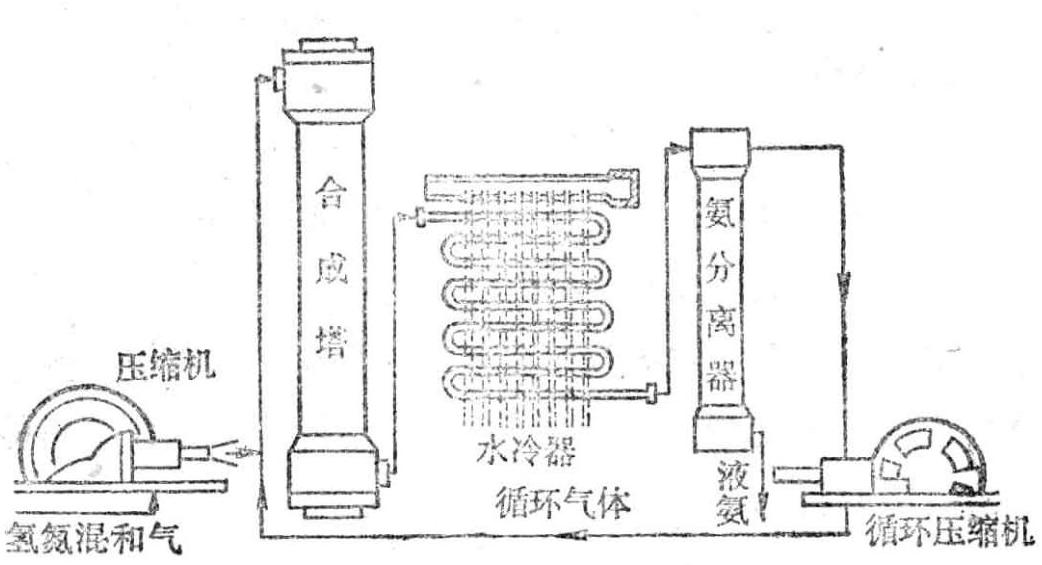
\includegraphics[max width=1.0\textwidth]{images/01912d13-9986-7822-a012-3f3f7be99dcb_95_786953.jpg}
\end{center}

\begin{itemize}
\item 图 3-6 合成氨的简要流程示意图
\end{itemize}

图中, 氮、氢混和气体经过压缩以后, 进入氨合成塔。化学反应在合成塔里进行, 这个反应是在高压、适当的温度和有触媒存在的条件下进行的放热反应。

合成塔的构造除为了有利于催化, 要能够安放厚层的触媒外, 还要能够耐高压和能够调节温度。为了符合这个要求, 合成塔有耐高压的厚壁。塔里主要有接触室和热交换器两部分。氨的合成塔种类很多。图 3-7 是一种合成塔的内部构造示意图。合成塔是一个具有厚壁的钢筒, 可以耐高压, 塔壳外用绝缘材料包裹。合成塔里上部为接触室, 内放粒状触媒, 下部是热交换器。

氮、氢混和气体是由塔的上部进入塔里, 向下沿着塔壳和接触室间的间隙流到下部热交换器。在热交换器里, 混和气体在管子和管子之间的空隙曲曲折折地向上流动, 同时, 吸收管子里反应后的热气体的热量, 这样混和气体的温度就逐渐升高。预热了的氮、氢混和气体由塔的上部中间的粗管流

\begin{center}
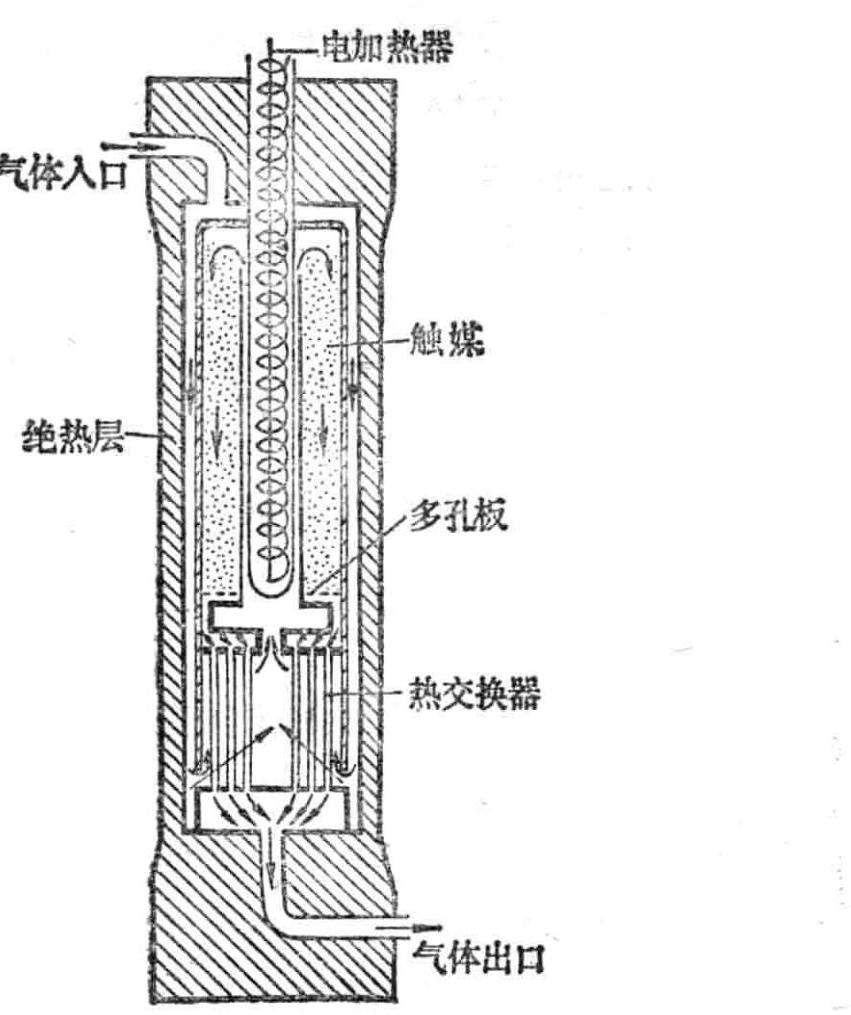
\includegraphics[max width=0.9\textwidth]{images/01912d13-9986-7822-a012-3f3f7be99dcb_96_587411.jpg}
\end{center}

图 3-7 一种合成塔的内部构造示意图

进接触室。然后由上而下地通过触媒层。这时即有一部分氮气和氢气化合成氨。反应后的气体经多孔板向下通入热交换器的管子, 被管外新导入的混和气体所冷却, 然后由气体出口离开合成塔。在正常工艺操作的情况下,反应放出的热量足以保持接触室的温度, 不需要另外供给热量。如果反应物里的杂质已经仔细清除掉, 触媒可以连续使用。

\section*{3. 氨的分离}

从合成塔里出来的混和气体,通常约含 \({15}\%\) 左右的氨。 为了使氨从没有起反应的氮气和氢气里分离出来, 要把混和气体通过冷凝器, 使氨液化, 然后在气体分离器里把液态氨分离出来, 导入液氨贮罐。由气体分离器出来的气体, 经过循环压缩机, 再送到合成塔里去。

使没有起反应的物质从反应后的生成物里分离出来, 并重新回到反应器里去的工艺过程, 叫做循环操作过程。利用循环操作过程, 即使平衡混和物里生成物的含量不很大, 也可以充分地利用原料来制造所需的生成物。

我国合成氨工业的发展很迅速, 它在支援农业生产、实现农业现代化中起着很重要的作用。我国合成氨工业不但在产量上不断提高, 而且在技术上也取得了比较显著的成就。

合成氨工业对化学工业和国防工业也都有重要的意义。

化学模拟生物固氮简介

我们已学习了合成氨的生产原理。我们也知道氨和许多铵盐都是很重要的化学肥料。这是因为氮是构成蛋白质的基本元素之一,是农作物生长的主要营养元素之一。自然界里含有大量的氮元素, 氮气占空气总体积的百分之七十八, 但却不能被植物直接利用。变成铵态的氮, 就能被植物吸收。但要把氢气和空气中的氮气转变成氨, 却正如前面介绍的需要高压和一定的高温才行。这就必须要有耐高压、高温的器材和设备, 还需要大量动力。那么能不能在常温常压条件下, 把空气中的氮转变为铵态氮呢? 人们在六十多年来曾进行了大量的努力, 希望在温和条件下实现氨的合成, 但一直还没有成功。然而, 我们知道某些豆科植物, 它们的根部有根瘤菌共生, 根瘤菌能起固氮作用, 即摄取空气中的氮转化成氨等, 为植物直接吸收, 这就叫做生物固氮现象, 生物固氮是在常温、 常压下进行的。实际上, 地球上的氮气的固定, 绝大部分是通过生物固氮进行的, 据不完全统计, 全世界工业合成氮肥中的氮只占固氮总量的百分之二十。那么,人们能不能向大自然学到这种本领呢? 这就需要研究如何模拟生物的功能, 把生物的功能的原理用于化学, 借以改善现有的并且创造崭新的化学工艺过程。如果模拟成功,不仅可以大大提高氮肥工业的效率, 发展农业生产, 同时还会对很多化学工业产生深远影响。

\section*{习 题}

1. 在氮、氢合成氨的反应达到平衡时, 反应混和物里各物质的浓度分别是: \(\left\lbrack {\mathrm{N}}_{2}\right\rbrack = 3\) 摩尔/升, \(\left\lbrack {\mathrm{H}}_{2}\right\rbrack = 8\) 摩尔/升, \(\left\lbrack {\mathrm{{NH}}}_{3}\right\rbrack = 4\) 摩尔/升。试求 \({\mathrm{N}}_{2}\text{、}{\mathrm{H}}_{2}\) 的起始浓度和这个反应的平衡常数。

2. 在制硫酸中,用空气来氧化 \({\mathrm{{SO}}}_{2}\) 生成 \({\mathrm{{SO}}}_{3}\) ,

\[
2{\mathrm{{SO}}}_{2} + {\mathrm{O}}_{2}\mathop{\div }\limits_{{{\mathrm{V}}_{2}{\mathrm{O}}_{5}}}^{{{400} - {500}^{ \circ }\mathrm{C}}}2{\mathrm{{SO}}}_{3} + {47}\text{千卡}
\]

为什么在生产上要用过量的空气, 使用催化剂, 并在适当的温度下进行?

\section*{内容提要}

化学反应速度是研究在单位时间内反应物或生成物浓度的变化, 化学平衡是研究反应进行的方向和反应进行的程度。 这两个问题对今后的化学学习和生产实践都是很重要的。

\section*{一、化学反应速度的表示方法}

化学反应速度通常是用单位时间内反应物浓度的减小或生成物浓度的增大来表示。浓度一般用摩尔/升表示; 时间可以根据反应的快慢用秒、分或小时来表示。

\section*{二、影响化学反应速度的重要条件}

反应物能不能发生化学反应以及反应的快慢, 首先决定于反应物质的性质。此外, 化学反应速度还受反应进行时所处条件的影响, 其中重要的是温度、浓度、压强和催化剂。

要反应物相互作用, 必须使反应物分子相互碰撞, 碰撞的分子要具有足够的能量, 才能发生化学反应。这种能够发生化学反应的分子碰撞, 叫做有效碰撞。活化分子具有的最低能量与分子平均能量的差叫做活化能。反应物分子中活化分子的百分数越大,有效碰撞的次数越多,反应进行得就越快。所以, 一个反应进行的快慢, 决定于有效碰撞的次数。而增加反应的温度、浓度、压强 (气体反应) 和使用性能良好的催化剂, 都能增加反应物分子间的有效碰撞次数, 因而都能增大反应的速度。

\section*{三、化学平衡及化学平衡的移动}

在一定温度下, 一个密闭容器里进行的可逆反应, 当正反应和逆反应的反应速度相等时, 达到化学平衡。化学平衡是一种动态平衡。在平衡时, 反应混和物中各组成物质的浓度保持不变。

对于一般的可逆反应

\[
m\mathrm{\;A} + n\mathrm{\;B} \rightleftharpoons p\mathrm{C} + q\mathrm{D}
\]

当达到平衡时, 各反应物质的浓度满足下面的关系式:

\[
\frac{{\left\lbrack \mathrm{C}\right\rbrack }^{p}{\left\lbrack \mathrm{D}\right\rbrack }^{q}}{{\left\lbrack \mathrm{\;A}\right\rbrack }^{m}{\left\lbrack \mathrm{\;B}\right\rbrack }^{n}} = K
\]

\(K\) 叫做这个反应的平衡常数。平衡常数随温度的不同而改变。

平衡移动原理(勒沙特列原理): 如果改变影响平衡的一个条件 (如浓度、温度、压强等), 平衡就向能够使这种改变减弱的方向移动。还可具体分述如下:

\[
\text{浓度}\left\{ \begin{array}{l} \text{ 增大反应物浓度或减小生成物浓度 } \\ \text{ 反应方向移动 } \\ \text{ 减小反应物浓度或增大生成物浓度 } \\ \text{ 反应方向移动 } \end{array}\right. \text{平衡向逆}
\]

温度 \(\left\{ \begin{array}{l} \text{ 升高温度 } \\ \text{ 降低温度 } \end{array}\right.\) -平衡向吸热方向移动

压强 \(\left\{ \begin{array}{l} \text{增大压强 } \\ \text{ 减小压强 } \end{array}\right.\) 平衡向气态物质体积缩小方向移动

催化剂对化学平衡的移动没有影响。

\section*{四、合成氨反应及其适宜的条件}

由于用氮气和氢气合成氨的反应中, 气体体积缩小和氮分子的不活动性, 合成氨的工业生产过程需要在高压、适当温度(因系放热反应, 温度不能过高)和有催化剂存在的条件下进行。

\section*{复习强}

\section*{1. 某一化学反应}

\[
\mathrm{A} + \mathrm{B} \rightarrow \mathrm{C}
\]

开始时, \(\mathrm{A}\) 的浓度为 2 摩尔/升,两分钟后反应达到平衡, \(\mathrm{A}\) 的浓度下降为 1.5 摩尔/升,求这个反应以 \(\mathbf{A}\) 的浓度变化来表示的反应速度是多少?

2. 在 \({\mathrm{N}}_{2} + 3{\mathrm{H}}_{2} \rightleftharpoons 2{\mathrm{{NH}}}_{3}\) 反应里,经 2 秒钟后, \({\mathrm{{NH}}}_{3}\) 的浓度增大了 0.6 摩尔/升,那末,在这 2 秒钟内,用 \({\mathrm{H}}_{2}\) 浓度变化表示的反应速度是多少?

3. 把 \({\mathrm{{HgCl}}}_{2}\) 的晶体和 \(\mathrm{{KI}}\) 的晶体放在研钵中研磨,能缓慢地起反应,颜色逐渐变红。如果把 \({\mathrm{{HgCl}}}_{2}\) 溶液和 \(\mathrm{{KI}}\) 溶液混和,立即生成红色 \({\mathrm{{HgI}}}_{2}\) 沉淀。为什么?

4. 下列数据是一些反应的平衡常数, 试判断, 哪个反应进行得最接近完全?哪个反应进行得最不完全?

\[
K = 1\;K = {10}\;K = {10}^{-1}\;K = {10}^{10}\;K = {10}^{-{10}}
\]

5. 下列说法对不对? 为什么?

(1)当可逆反应达到平衡时, 逆反应就停止了。

(2)在合成氨的反应中使用催化剂,可使氮的转化率提高。

(3)温度升高, 使吸热反应速度增大, 使放热反应速度减小。

(4) 当温度不变时, 增大反应物的浓度, 使平衡常数减小; 增大生成物的浓度, 使平衡常数增大。

(5)增大压强对溶液中的酸碱中和反应没有什么影响。

6. 在某温度时, \({\mathrm{H}}_{2} + {\mathrm{I}}_{2} \rightleftharpoons 2\mathrm{{HI}}\) 的平衡常数是 50 。在这温度下, 使氢与碘蒸气发生反应。反应开始时, 碘蒸气的浓度是 1 摩尔/升。当达到平衡时, 碘化氢的浓度为 0.9 摩尔/升, 求反应开始时氢的浓度是多少?

\section*{7. 已知反应}

\({\mathrm{H}}_{2}\left( \text{气}\right) + {\mathrm{I}}_{2}\left( \text{气}\right) \rightleftharpoons 2\mathrm{{HI}}\left( \text{气}\right)\) 在某温度达到平衡时,平衡常数 \(K = {62.5}\) ,如果在一个 10 升的容器里放入 5 摩尔 \({\mathrm{H}}_{2}\) 和 5 摩尔 \({\mathrm{I}}_{2}\) ,于该温度达到平衡,计算平衡时 \({\mathrm{H}}_{2}\text{、}{\mathrm{I}}_{2}\) 和 \(\mathrm{{HI}}\) 的浓度。

8. \(2\mathrm{{HI}}\) (气) \(\rightleftharpoons {\mathrm{H}}_{2}\) (气) \(+ {\mathrm{I}}_{2}\) (气) 在 \({500}^{ \circ }\mathrm{C}\) 时的 \(K =\) 0.016。若反应开始时,在一个 2 升容器内放入 1 摩尔 \(\mathrm{{HI}}\) ,求达到平衡时 \({\mathrm{H}}_{2}\text{、}{\mathrm{I}}_{2}\) 和 \(\mathrm{{HI}}\) 的浓度。

9. 在硫酸生产中, 二氧化硫氧化生成三氧化硫的反应如下:

\[
2{\mathrm{{SO}}}_{2} + {\mathrm{O}}_{2} \rightleftharpoons 2{\mathrm{{SO}}}_{3} + {47}\text{千卡}
\]

回答以下问题:

(1)升高温度对上述反应有什么影响?为什么工业上常在 \({400} - {500}^{ \circ }\mathrm{C}\) 下进行反应?

(2)增大压强对上述反应有什么影响?为什么工业上常在接近常压下操作?

(3)从沸腾炉导出的炉气在进入接触室之前, 为什么要进行除尘、洗涤、干燥等净化措施?

(4)进入接触室的原料气中, 为什么空气常是过量的?

(5)为什么要用适当的催化剂如五氧化二钒?

(6)从吸收塔放出的尾气中, 为什么仍含有少量二氧化硫?

\section*{第四章 硅 胶体}

\section*{第一节 碳族元素}

碳族元素属于元素周期表的第 IV 主族, 包括碳、硅、锗、 锡、铅五种元素。碳族元素的原子序数、原子量和它们的原子的电子层排布如表 4-1 所示。

第 IV 主族元素位于周期表里容易失去电子的主族元素和容易得到电子的主族元素的中间位置, 容易生成共价化合物。

碳族元素原子的最外层电子排布式是 \(n{s}^{2}n{p}^{2}\) ,随着电子层的增加, 碳族元素的性质呈规律性的变化。表 4-2 列出了碳族元素的一些重要性质。

碳族元素随着电子层和核电荷数的增加, 它们的一些重要物理性质和化学性质都发生规律性的变化。它们从上到下由非金属性向金属性递变的趋势比氮族元素更为明显。碳是明显的非金属; 硅虽然外貌象金属, 但在化学反应中更多地显非金属性, 通常被认为是非金属; 锗的金属性比非金属性强; 锡和铅都是金属。

碳族元素的电负性比同一周期的卤族、氧族和氮族的小。

碳族元素的化合价除 +4 价外, 还有 +2 价。碳、硅、锗、 锡的 +4 价化合物是稳定的, 而铅的 +2 价化合物是稳定的。

半群国土审印大堂叱喜士当`孫冶士劉卯迷壬郭激 I-i 辛

\begin{center}
\adjustbox{max width=\textwidth}{
\begin{tabular}{|c|c|c|c|c|c|}
\hline
\({\rho }_{1}\) O & \phantom{X} & \phantom{X} & \phantom{X} & 5.5\% & (S3) orProduss \\
\hline
Z & \phantom{X} & \phantom{X} & \phantom{X} & \phantom{X} & reflect to \({d}_{{V}_{3}}{s}_{V}\) \\
\hline
外 & \phantom{X} & \phantom{X} & (2, 2) & 01.21, d \({\bar{v}}_{\bar{v}}\) s v & \phantom{X} \\
\hline
核 服 原 & \phantom{X} & STRATE & OIPCATSISS & OIPSOUSISE & 01 \({p}_{{\text{S}}_{9}}d\) SzS E \\
\hline
1 & \includegraphics[max width=0.2\textwidth]{images/01912d13-9986-7822-a012-3f3f7be99dcb_104_464508.jpg} & 2.2021 & 2.2, 2.1 & 2.7.2 & 2.27 \\
\hline
区 & 5.5 & 5.00 & 3.5 & 0.01 & 1.00 \\
\hline
區子區 & 1,011 & 2.0\% & 72.5\% & 0.0 & 2Q2 \\
\hline
将来 & 6 & 1. & C1 & S & 83 \\
\hline
合動筆空 & (1) & is & C & S & 孔 \\
\hline
城牙第三 & 碳 & 硅 & 销 & 锡 & 铅 \\
\hline
\end{tabular}
}
\end{center}

表 4-2 碳族元素的一些重要性质

\begin{center}
\adjustbox{max width=\textwidth}{
\begin{tabular}{|c|c|c|c|c|c|c|c|}
\hline
\multicolumn{4}{|c|}{\phantom{X}} & \multicolumn{4}{|c|}{单质的性质} \\
\cline{1-4}
\multirow{2}{*}{元素} & \multirow{2}{*}{原子半径 (10-10米)} & \multirow{2}{*}{第一电商能 (电子伏特)} & \multirow{2}{*}{主要化合价} & \multicolumn{4}{|c|}{\phantom{X}} \\
\cline{5-8}
& & & & 状态和颜色 & 密度(克/厘米) & 熔点(℃) & 沸点 \(\left( {{}^{ \circ }\mathrm{C}}\right)\) \\
\hline
碳 & 0.77 & 11.3 & \(+ 2, + 4\) & 无色或黑色圆体 & 3.51(c) 2. \({25}^{ \oplus }\) & 3550 3652-97(升华) & 4827 4827 \\
\hline
硅 & 1.17 & 8.2 & \(\rightarrow \frac{1}{2} + \frac{4}{2}\) & 从无色到棕色固体 & \(2,{32} - 2,{34}\) & 1410 & 2355 \\
\hline
错 & 1.22 & 7.9 & \(+ 2, + 4\) & 灰白色固体 & 5.35 & 937.4 & 2330 \\
\hline
锡 & 1.41 & 7.3 & \(+ 2, + 4\) & 银白色固体 & 7.28 & 231.9 & 2260 \\
\hline
铅 & 1.75 & 7.4 & \(+ 2, + 4\) & 蓝白色固体 & 11.34 & 327.5 & 1740 \\
\hline
\end{tabular}
}
\end{center}

② 石墨 ① 金刚石

在自然界里, 碳族元素以不同的形态存在。碳有游离态的碳, 如金刚石、石墨、无定形碳等, 也有化合态的碳, 如各种碳酸盐和大量的有机化合物中的碳。地壳中碳的含量虽然不多, 但它是地球上形成化合物种类最多的元素。硅在地壳中主要以含氧化合物矿石的形式存在。锗是不常见的元素, 通常它与若干金属同时存在于硫化物矿内。锡和铅两种金属在自然界都以化合态存在。锡的主要矿石是锡石矿 \(\left( {\mathrm{{SnO}}}_{2}\right)\) ,铅的主要矿石是方铅矿(PbS)。

在初中化学里我们已学习过碳元素, 下面将着重介绍硅及其重要化合物, 锗、锡、铅就不再介绍了。

\section*{习 题}

1. 画出硅的原子结构简图, 写出硅的电子式以及主要化合价, 说明硅在自然界的存在方式。

2. 说明碳、硅的化合物为什么大多数以共价键相结合。

\section*{第二节 硅及其重要的化合物}

\section*{一、硅}

我们已经知道, 在地壳里, 硅的含量在所有元素中居第二位, 仅次于氧。自然界里没有游离态的硅, 而只有化合态的硅。化合态的硅几乎全部是二氧化硅和硅酸盐, 它们广泛地存在于地壳的各种矿物和岩石里。硅是构成矿物与岩石的主要元素。

1. 物理性质

晶体硅是无色到棕色有金属光泽、硬而脆的固体(表 4- 2)。硅原子最外电子层的结构是 \(3{s}^{2}3{p}^{2}\) ,有 4 个价电子。晶体硅的结构与金刚石结构相似, 每个硅原子跟另外 4 个硅原子形成 4 个共价键, 成为正四面体结构。这种结构跟金刚石结构相似, 也是一种网状的原子晶体 (图 4-1)①。这样就决定了硅的硬度较大, 熔点和沸点较高。但是由于硅的原子半径比碳大, 晶体硅里 \(\mathrm{{Si}} - \mathrm{{Si}}\) 的键长 \(\left( {{2.35} \times {10}^{-{10}}}\right.\) 米 \()\) 大于金刚石里 \(\mathrm{C} - \mathrm{C}\) 的键长; 而 \(\mathrm{{Si}} - \mathrm{{Si}}\) 的键能 (42.5 千卡/摩尔) 小于金刚石里 \(\mathrm{C} - \mathrm{C}\) 的键能。所以,晶体硅的硬度、熔点和沸点都小于或低于金刚石。

\begin{center}
\includegraphics[max width=0.4\textwidth]{images/01912d13-9986-7822-a012-3f3f7be99dcb_106_252125.jpg}
\end{center}

图 4-1 晶体硅结构的平面示意图

硅的导电性能介于金属和绝缘体之间。硅是良好的半导体材料, 可用来制造半导体器件, 如硅整流器、晶体管和集成电路等。

锗和硅相似, 也是重要的半导体材料。

\section*{2. 化学性质}

硅是非金属元素, 硅的许多化学性质和碳相似, 它跟其它元素化合时形成共价键。

硅的化学性质不活泼。在常温下, 除氟气、氢氟酸和强碱溶液外, 其它物质如氧气、氯气、硫酸和硝酸等都不跟硅起反应。在加热条件下, 硅能跟一些非金属起反应, 例如, 把硅研细后加热, 它就燃烧生成二氧化硅, 同时放出大量的热。

\[
\mathrm{{Si}} + {\mathrm{O}}_{2} \triangleq {\mathrm{{SiO}}}_{2}
\]

\customfootnote{

① 图 4-1 是平面图, 晶体硅实际上是立体结构。

}

硅能跟强碱溶液作用生成硅酸盐, 放出氢气。

\[
\mathrm{{Si}} + 2\mathrm{{NaOH}} + {\mathrm{H}}_{2}\mathrm{O} = {\mathrm{{Na}}}_{2}{\mathrm{{SiO}}}_{3} + 2{\mathrm{H}}_{2} \uparrow
\]

在一般情况下, 硅跟氢气不能直接化合。硅的氢化物常用间接方法制得。

象碳一样, 硅还能跟某些金属生成硅化物, 所以, 硅可用来制造合金。如炼钢时常用硅铁合金做脱氧剂来除氧; 含硅 \(4\%\) 的钢有导磁性,可以用来制造变压器的铁芯; 含硅 \({15}\%\) 左右的钢有耐酸性, 可以用来制造耐酸设备。

工业上, 硅是在电炉里用碳还原二氧化硅而制得的。

\[
{\mathrm{{SiO}}}_{2} + 2\mathrm{C}\xrightarrow[]{\text{ 高温 }}\mathrm{{Si}} + 2\mathrm{{CO}} \uparrow
\]

这样制得的硅是含少量杂质的粗硅。粗硅提纯后, 可制得作为半导体材料的高纯硅。

\section*{二、二氧化硅}

\section*{1. 物理性质}

二氧化硅 \(\left( {\mathrm{{SiO}}}_{2}\right)\) 是一种坚硬难熔的固体,它和其它矿物构成了多种岩石, 广泛地分布在自然界里。

天然的二氧化硅分为晶体和无定形两大类。石英的主要成分就是二氧化硅晶体。自然界纯净的石英是无色透明的六方柱状晶体, 这种晶体就是我们常说的水晶。

硅藻土含有无定形二氧化硅, 它是死去的硅藻 \(\Phi\) 及其它微小生物的遗体经沉积胶结而成的多孔、质轻、松软的固体物质。它的表面积很大, 吸附能力较强, 可作吸附剂和催化剂的载体 \({}^{\left( 1\right) }\) ,以及保温材料等。

\customfootnote{

① 硅藻是单细胞的低等水生植物。

}

二氧化硅和二氧化碳在物理性质上有很大的差别。例如, 二氧化硅的熔点高、硬度大; 而二氧化碳在通常状况下是气体, 固体二氧化碳的熔点很低, 等等。二氧化硅和二氧化碳的这些差别是由它们的不同结构决定的。我们已经知道固体二氧化碳是一种分子晶体。分子间只有较小的分子间引力, 所以,它的熔点很低。但是二氧化硅却不是由单个的 “ \({\mathrm{{SiO}}}_{2}\) ” 的分子所组成的分子晶体, 而是一种原子晶体。如图 4-2②所示, 1 个 \(\mathrm{{Si}}\) 原子跟 4 个 \(\mathrm{O}\) 原子形成了 4 个共价键,这样,每 1 个 \(\mathrm{{Si}}\) 原子周围结合 4 个 \(\mathrm{O}\) 原子; 同时,每个 \(\mathrm{O}\) 原子跟两个 \(\mathrm{{Si}}\) 原子相结合。实际上, 二氧化硅晶体是由硅原子和氧原子按 \(1 : 2\) 的比率所组成的立体网状的原子晶体, 我们通常用化学式 \({\mathrm{{SiO}}}_{2}\) 来表示二氧化硅的组成。在二氧化硅的晶体里 \(\mathrm{{Si}} - \mathrm{O}\) 的键长为 \({1.62} \times {10}^{-{10}}\) 米,键能为 88.2 千卡/摩尔。由于二氧化硅晶体里 \(\mathrm{{Si}} - \mathrm{O}\) 键的键能很高,并形成了一种立体网状的原子晶体, 所以, 要使它熔融, 也就是说要破坏二氧化硅的晶体, 必须消耗较多的能量, 因此, 二氧化硅的熔点很高, 硬度也很大。

\begin{center}
\includegraphics[max width=0.5\textwidth]{images/01912d13-9986-7822-a012-3f3f7be99dcb_108_796814.jpg}
\end{center}

图 4-2 二氧化硅晶体平面示意图

\customfootnote{

① 为了增加催化剂的有效面积, 一般使催化剂附着于多孔的物体表面, 这种多孔物体叫做载体。

② 图 4-2 是一个简化的平面示意图, 实际上二氧化硅晶体是立体的网状结构。

}

\section*{2. 化学性质}

由于二氧化硅的 \(\mathrm{{Si}} - \mathrm{O}\) 键能很大,因而它的化学性质十分稳定, 不能跟酸 (除氢氟酸外) 发生反应。二氧化硅是一种酸性氧化物。但是, 二氧化硅不溶于水, 它不能跟水起反应生成酸。二氧化硅能跟碱性氧化物或强碱反应生成盐。

\[
{\mathrm{{SiO}}}_{2} + {\mathrm{{CaO}}}^{\text{高温 }}{\mathrm{{CaSiO}}}_{3}
\]

\[
{\mathrm{{SiO}}}_{2} + 2\mathrm{{NaOH}} = {\mathrm{{Na}}}_{2}{\mathrm{{SiO}}}_{3} + {\mathrm{H}}_{2}\mathrm{O}
\]

玻璃中含有二氧化硅, 因而它能被碱液腐蚀。实验室中盛放碱液的试剂瓶常用橡皮塞, 而不用玻璃塞, 就是为了防止玻璃受碱液腐蚀生成 \({\mathrm{{Na}}}_{2}{\mathrm{{SiO}}}_{3}\) ,而使瓶口和塞子粘在一起。

\section*{3. 用途}

二氧化硅的用途很广。自然界里比较稀少的水晶可用以制造电子工业的重要部件、光学仪器和工艺品。

二氧化硅是制造光导纤维的重要原料。

一般较纯净的石英, 可用来制造石英玻璃。石英玻璃的膨胀系数很小,相当于普通玻璃的 \(1/{18}\) ,能经受温度的剧变, 耐酸性能好 (除 HF 外)。因此, 石英玻璃常用来制造耐高温的化学仪器。

石英砂常用作玻璃原料和建筑材料。

\section*{三、硅酸 硅酸盐}

1. 硅酸

硅酸不能用二氧化硅跟水直接作用制得, 而只能用相应的可溶性的硅酸盐跟酸作用制得。

硅酸钠 \(\left( {{\mathrm{{Na}}}_{2}{\mathrm{{SiO}}}_{3}}\right) \text{①}\) 的水溶液跟盐酸起反应生成的白色胶状沉淀叫做原硅酸,通常用 \({\mathrm{H}}_{4}{\mathrm{{SiO}}}_{4}\) 来表示它的组成。原硅酸几乎不溶于水, 是一种弱酸, 很不稳定。这种白色胶状物在空气里干燥, 失去一部分水后, 变成白色粉末。这种物质是硅酸,通常用 \({\mathrm{H}}_{2}{\mathrm{{SiO}}}_{3}\) 来表示它的组成 (可以认为是 \({\mathrm{H}}_{4}{\mathrm{{SiO}}}_{4} =\) \({\mathrm{H}}_{2}{\mathrm{{SiO}}}_{3} + {\mathrm{H}}_{2}\mathrm{O}\) )。硅酸不溶于水,也是一种弱酸,它的酸性比碳酸还弱。

\section*{2. 硅酸盐}

硅酸、原硅酸以及由它们缩水结合而成的各种酸所对应的盐,统称硅酸盐。例如,硅酸钠 \(\left( {{\mathrm{{Na}}}_{2}{\mathrm{{SiO}}}_{3}}\right)\) 、镁橄榄石 \(\left( {{\mathrm{{Mg}}}_{2}{\mathrm{{SiO}}}_{4}}\right)\) 、高岭石 \(\left\lbrack {{\mathrm{{Al}}}_{2}\left( {{\mathrm{{Si}}}_{2}{\mathrm{O}}_{5}}\right) {\left( \mathrm{{OH}}\right) }_{4}}\right\rbrack\) 等都是硅酸盐。硅酸盐种类很多, 结构也很复杂, 它是构成地壳岩石的最主要成分。我们可以用二氧化硅和金属氧化物的形式表示硅酸盐的组成。例如:

硅酸钠 \({\mathrm{{Na}}}_{2}{\mathrm{{SiO}}}_{3}\;\left( {{\mathrm{{Na}}}_{2}\mathrm{O} \cdot {\mathrm{{SiO}}}_{2}}\right)\)

镁橄榄石 \({\mathrm{{Mg}}}_{2}{\mathrm{{SiO}}}_{4}\left( {2\mathrm{{MgO}} \cdot {\mathrm{{SiO}}}_{2}}\right)\)

高岭石 \({\mathrm{{Al}}}_{2}\left( {{\mathrm{{Si}}}_{2}{\mathrm{O}}_{5}}\right) {\left( \mathrm{{OH}}\right) }_{4}\;\left( {{\mathrm{{Al}}}_{2}{\mathrm{O}}_{3} \cdot 2{\mathrm{{SiO}}}_{2} \cdot 2{\mathrm{H}}_{2}\mathrm{O}}\right)\)

许多硅酸盐都是难溶于水的。可溶性硅酸盐中, 最常见的是 \({\mathrm{{Na}}}_{2}{\mathrm{{SiO}}}_{3}\) ,它的水溶液俗名水玻璃。水玻璃是无色粘稠的液体, 是一种矿物胶, 它既不能燃烧也不受腐蚀, 在建筑工业上可用作粘合剂、耐酸水泥掺料等。木材、织物浸过水玻璃后, 具有防腐性能, 且不易着火。水玻璃还可用作耐火材料。

\customfootnote{

① \({\mathrm{{Na}}}_{2}{\mathrm{{SiO}}}_{3}\) 通常也叫偏硅酸钠,现在根据 1982 年版《无机化学命名原则》称为硅酸钠。

}

粘土的成分也是硅酸盐。花岗岩里的正长石 \(\left( {{\mathrm{{KAlSi}}}_{3}{\mathrm{O}}_{8}}\right)\) 在二氧化碳和水的作用下, 分解而生成粘土等物质。粘土的种类很多, 成分也很复杂 (主要是高岭石), 它是土壤里矿物质的主要部分。 常见的有高岭土 \({}^{\left( 1\right) }\) 和一般粘土,前者含杂质较少, 后者含杂质较多。

\section*{习 题}

1. 粗硅提纯时常用下述方法: 将粗硅在高温下跟氯气反应生成四氯化硅 \(\left( {\mathrm{{SiCl}}}_{4}\right) ,{\mathrm{{SiCl}}}_{4}\) 经过分馏提纯,再用氢气还原得到纯硅。写出上述反应的化学方程式。

2. 晶体硅和金刚石在结构和物理性质上有哪些相似的地方, 有哪些不同的地方?

3. 二氧化碳和二氧化硅在物理性质方面有什么不同, 试从结构角度加以说明。

4. 怎样用化学方法检验生石灰里混有的石英和石灰石等杂质? 写出有关的化学方程式。

5. 往电炉里加入 60 克 \({\mathrm{{SiO}}}_{2}\) 和 20 克碳的混和物,通电, 使它们发生如下反应: \({\mathrm{{SiO}}}_{2} + 2\mathrm{C} = \mathrm{{Si}} + 2\mathrm{{CO}}\) 。求:

(1) 生成物的质量各多少克?

(2)生成的 \(\mathrm{{CO}}\) 在标准状况下是多少升?

\customfootnote{

① 高岭土又叫瓷土, 主要由高岭石的微细晶体组成, 因盛产于我国江西景德镇的高岭而得名。

}

6. 把下列式子改写成氧化物的形式:

(1) 高岭石 \(\left\lbrack {{\mathrm{{Al}}}_{2}\left( {{\mathrm{{Si}}}_{2}{\mathrm{O}}_{5}}\right) {\left( \mathrm{{OH}}\right) }_{4}}\right\rbrack\)

(2) 滑 石 \(\left\lbrack {{\mathrm{{Mg}}}_{3}\left( {{\mathrm{{Si}}}_{4}{\mathrm{O}}_{10}}\right) {\left( \mathrm{{OH}}\right) }_{2}}\right\rbrack\)

(3) 钙沸石 \(\left\lbrack {\mathrm{{Ca}}\left( {{\mathrm{{Al}}}_{2}{\mathrm{{Si}}}_{3}{\mathrm{O}}_{10}}\right) \cdot 3{\mathrm{H}}_{2}\mathrm{O}}\right\rbrack\)

7. 怎样用石英和其它物质制取硅酸? 写出相应的化学方程式。

\section*{第三节 硅酸盐工业简述}

以含硅物质为原料, 经过加热制成硅酸盐产品的工业, 如制造水泥、玻璃、陶瓷等产品的工业, 叫做硅酸盐工业。它在国民经济中占有重要的地位。

\section*{一、水泥}

普通硅酸盐水泥的主要原料是石灰石和粘土。先把石灰石、粘土和其它辅助原料按一定的比率混和, 磨细成生料, 将生料装入回转窑里煅烧(图 4-3)。

\begin{center}
\includegraphics[max width=1.0\textwidth]{images/01912d13-9986-7822-a012-3f3f7be99dcb_112_754524.jpg}
\end{center}

图 4-3 水泥回转窑示意图

煅烧时, 燃料从回转窑的低端喷入, 原料从回转窑的高端流入。借原料本身的重力作用逐渐下移, 经过预热带、煅烧带和烧结带 (温度可达 \({1400} - {1500}^{ \circ }\mathrm{C}\) )。原料在高温下,发生了复杂的物理、化学变化, 成为部分熔化状态, 冷却后成为硬块, 这种物质叫做熟料, 再加入适量的石膏 (调节水泥硬化速度), 磨成细粉, 即制成普通硅酸盐水泥。这种水泥的主要成分有:

硅酸三钙 \(3\mathrm{{CaO}} \cdot {\mathrm{{SiO}}}_{2}\)

硅酸二钙 \(2\mathrm{{CaO}} \cdot {\mathrm{{SiO}}}_{2}\)

铝酸三钙 \(3\mathrm{{CaO}} \cdot {\mathrm{{Al}}}_{2}{\mathrm{O}}_{3}\)

水泥实际上是上述主要成分的混和物, 水泥的组成和结晶形态的不同直接影响到它的各种主要性能。

水泥具有水硬性. 水泥跟水拌和后, 发生作用, 生成不同的水合物, 同时放出一定的热量。生成的水合物逐步形成胶状物, 并开始凝聚, 最后, 有些胶状物转变为晶体, 使胶状物和晶体交错地结合起来, 成为强度很大的固体。这个过程叫做水泥的硬化。水泥不论是在空气中还是在水中都能硬化, 所以, 它不仅是一般的建筑材料, 而且还是水下工程必不可少的建筑材料。

为了改善水泥的性能, 扩大水泥的使用范围, 可在硅酸盐水泥熟料里, 掺入适当比率的混和材料, 制成各种水泥。例如, 矿渣硅酸盐水泥就是在硅酸盐水泥熟料里加入一定量的高炉矿渣 (主要成分是 \({\mathrm{{CaSiO}}}_{3}\) ),沸石岩水泥就是在水泥熟料里掺入一定量的沸石岩。

水泥、砂子和水的混和物叫做水泥砂浆, 在建筑上用它作粘合剂, 能把砖、石等粘结起来。水泥、砂子、碎石和水按一定比率的混和物硬化后叫做混凝土, 常用它来建筑桥梁、厂房等巨大建筑物。水泥的热膨胀系数几乎跟铁一样, 所以用混凝土建造建筑物常用钢筋作结构, 使建筑物更加坚固, 这叫做钢筋混凝土。 1

\section*{二、玻璃}

制造普通玻璃的主要原料是纯碱 \(\left( {{\mathrm{{Na}}}_{2}{\mathrm{{CO}}}_{3}}\right)\) 、石灰石 \(\left( {\mathrm{{CaCO}}}_{3}\right)\) 和石英 \(\left( {\mathrm{{SiO}}}_{2}\right)\) ,有些特种玻璃原料中还包含氧化铅 (PbO) 和硼砂 \(\left( {{\mathrm{{Na}}}_{2}{\mathrm{\;B}}_{4}{\mathrm{O}}_{7} \cdot {10}{\mathrm{H}}_{2}\mathrm{O}}\right)\) 。生产玻 璃时,把原料粉碎, 按适当比混和以后, 放入玻璃熔炉里, 加强热。原料熔融后发生了比较复杂的物理、化学变化, 其中主要的反应是二氧化硅跟碳酸钠和碳酸钙起反应生成硅酸盐和二氧化碳:

\[
{\mathrm{{Na}}}_{2}{\mathrm{{CO}}}_{3} + {\mathrm{{SiO}}}_{2}\xrightarrow[]{\text{ 高温 }}{\mathrm{{Na}}}_{2}{\mathrm{{SiO}}}_{3} + {\mathrm{{CO}}}_{2} \uparrow
\]

\[
{\mathrm{{CaCO}}}_{3} + {\mathrm{{SiO}}}_{2}\xrightarrow[]{\text{ 高温 }}{\mathrm{{CaSiO}}}_{3} + {\mathrm{{CO}}}_{2} \uparrow
\]

在原料里,石英的用量是较多的。所以,普通玻璃是 \({\mathrm{{Na}}}_{2}{\mathrm{{SiO}}}_{3}\text{、}{\mathrm{{CaSiO}}}_{3}\) 和 \({\mathrm{{SiO}}}_{2}\) 熔化在一起所得到的物质。这种物质不是晶体, 称作玻璃态物质, 它没有一定的熔点, 而是在某一温度范围内逐渐软化。在软化状态时, 玻璃可以制成任何形状的制品。

玻璃的种类很多, 除上述普通玻璃外, 还有硼酸盐玻璃, 它是耐热仪器玻璃, 膨胀系数小, 能够耐骤冷、骤热, 化学稳定性好, 能耐酸、碱的腐蚀, 可用于制造化学仪器。铅玻璃折光率强, 常用于制作光学仪器等。制造有色玻璃, 一般是在原料里加入某些金属氧化物, 使金属氧化物均匀地分散到玻璃态的物质里,使玻璃呈现出特征颜色。例如,加氧化钴 \(\left( {{\mathrm{{Co}}}_{2}{\mathrm{O}}_{3}}\right)\) 呈蓝色; 加氧化亚铜 \(\left( {{\mathrm{{Cu}}}_{2}\mathrm{O}}\right)\) 呈红色,等等。

把普通玻璃放入电炉里加热, 使它软化, 然后急速冷却, 得到钢化玻璃。钢化玻璃的机械强度比普通玻璃大 4-6 倍, 不易破碎。破碎时碎块没有尖锐的棱角, 不易伤人, 可用来制造汽车或火车的车窗等。

玻璃还可以制成纤维。它具有较高的强度, 可作隔音、隔热、电气绝缘材料, 也可制造玻璃纤维增强塑料等等。

\section*{习 题}

1。制造普通玻璃的主要原料在玻璃窑里熔化后, 发生了哪些主要化学反应? 写出反应的化学方程式。

2. 普通玻璃含有 \({13}\;\%\) 的 \({\mathrm{{Na}}}_{2}\mathrm{O}\text{、}{11.7}\;\%\) 的 \(\mathrm{{CaO}}\text{、}{75.3}\;\%\) 的 \({\mathrm{{SiO}}}_{2}\) 。试计算三种氧化物的物质的量之比。

3. 制造一吨普通玻璃, 需要纯碱、石灰石和二氧化硅各多少吨(参看第 2 题得到的物质的量之比)? 并计算生产一吨普通玻璃,在温度为 \({1200}^{ \circ }\mathrm{C}\) 、压强为 750 毫米汞柱时,产生的二氧化碳是多少升?

\section*{第四节 胶 体}

在学习前几节时, 我们已经涉及有些物质在一定条件下形成了胶体。例如, 硅酸在水里形成的透明液体; 某些金属氧化物分散到玻璃态物质里形成有色玻璃等等。本节主要介绍什么是胶体和胶体的重要性质。

\section*{一、胶体}

在初中化学里我们已经学习过溶液、悬浊液和乳浊液。它们都是一种物质(或几种物质)的微粒分散于另一种物质里形成的混和物。我们常把这种混和物叫做分散系。其中分散成微粒的物质叫做分散质; 微粒分散在其中的物质叫做分散剂。例如, 对溶液来说, 溶质是分散质, 溶剂是分散剂, 溶液是一种分散系。悬浊液和乳浊液也是一种分散系, 其中的固体小颗粒或小液滴是分散质, 所用的溶剂是分散剂。

胶体也是一种分散系, 在这种分散系里, 分散质微粒直径的大小介于溶质的分子或离子的直径 (一般小于 \({10}^{-9}\) 米) 和悬浊液或乳浊液微粒的直径 (一般大于 \({10}^{-7}\) 米) 之间。一般地说,分散质微粒的直径大小在 \({10}^{-9} - {10}^{-7}\) 米之间的分散系, 叫做胶体。

[实验 4-1] 往一个烧杯里注入蒸馏水 20 毫升, 给烧杯加热使水沸腾,然后往沸水里滴加氯化铁 \(\left( {\mathrm{{FeCl}}}_{3}\right)\) 饱和溶液 1-2毫升。继续煮沸, 待溶液呈红褐色后, 停止加热。观察制得的胶体。

取一个大试管,注入 \({0.01}\mathrm{M}\) 碘化钾 \(\left( \mathrm{{KI}}\right)\) 的溶液 10 毫升, 用胶头滴管滴入 8-10 滴相同浓度的硝酸银 \(\left( {\mathrm{{AgNO}}}_{3}\right)\) 溶液, 边滴入边振荡。观察制得的胶体。

上面两个实验可分别用化学方程式表示如下:

\[
{\mathrm{{FeCl}}}_{3} + 3{\mathrm{H}}_{2}\mathrm{O} \triangleq \mathrm{{Fe}}{\left( \mathrm{{OH}}\right) }_{3}\text{(胶体)} + 3\mathrm{{HCl}}
\]

\[
\mathrm{{KI}} + {\mathrm{{AgNO}}}_{3} = \mathrm{{AgI}}\text{ (胶体) } + {\mathrm{{KNO}}}_{3}
\]

从这两个实验里可以分别看到, 氢氧化铁分散到水里所形成的胶体是红褐色的; 碘化银分散到水里所形成的胶体是浅黄色的。

这两种胶体的微粒分别是氢氧化铁或碘化银的许多分子的集合体 \(\text{①}\) ,它们的直径大小在 \({10}^{-9} - {10}^{-7}\) 米之间。

有些物质的分子直径很大, 达到了胶体微粒的大小, 并且能溶解于水(或其他溶剂)。这种物质溶于水 (或其他溶剂), 就形成了胶体,这种胶体的微粒是分子 \({}^{\text{②}}\) 。

我们常常根据胶体粒子大小介于 \({10}^{-9} - {10}^{-7}\) 米之间这一特点, 把不纯的胶体放进有半透膜 \({}^{\text{③}}\) 的容器内,让较小的微粒 (如分子、离子) 通过半透膜, 以净化胶体。

[实验 4-2] 用半透膜制成一个袋, 往这个袋里注入淀粉胶体 10 毫升和食盐溶液 5 毫升的混和液体, 然后如图 4-4所示用线把半透膜袋的上口缚好, 系在玻璃棒上, 并把它悬挂在盛有蒸馏水的烧杯里。

\begin{center}
\includegraphics[max width=0.4\textwidth]{images/01912d13-9986-7822-a012-3f3f7be99dcb_117_999898.jpg}
\end{center}

图 4-4 渗析

几分钟后, 用两个试管各取烧杯里的液体 5 毫升。往其中一个试管里注入少量硝酸银溶液; 往另一个试管里注入少量碘水。观察这两个试管里所发生的变化。

从实验可以看到,在加入硝酸银溶液的试管里出现了白色沉淀; 在加入碘水的试管里不发生变化。这就证明了氯离子可以透过半透膜的微孔, 而淀粉胶体的微粒不能透过半透膜的微孔。同样可以用实验证明, 钠离子也能透过半透膜。这种现象说明胶体微粒大于溶液里溶质的离子或分子。象这种把混有离子或分子杂质的胶体装入半透膜的袋里, 并把这个袋放在溶剂中, 从而使离子或分子从胶体溶液里分离的操作叫做渗析。应用渗析的方法可精制某些胶体。

\customfootnote{

① 这种胶体也叫粒子胶体。

② 这种胶体也叫分子胶体。

③ 半透膜: 一般指动物的膀胱膜、肠衣、羊皮纸、胶棉薄膜、玻璃纸等。半透膜有非常小的细孔, 这些细孔只能使离子或分子透过而不能使胶体微粒透过。

}

胶体的种类很多, 按照分散剂的不同, 可分为液溶胶、气溶胶和固溶胶。分散剂是液体的, 叫做液溶胶(也叫溶胶), 例如,上面实验里制备的 \(\mathrm{{Fe}}{\left( \mathrm{{OH}}\right) }_{3}\) 和 \(\mathrm{{AgI}}\) 胶体都是液溶胶。分散剂是气体的, 叫做气溶胶, 例如, 雾、云、烟等都是气溶胶。分散剂是固体的, 叫做固溶胶, 例如, 烟水晶、有色玻璃等都是固溶胶。

\section*{二、胶体的重要性质}

从外观看胶体跟溶液并没有明显区别。胶体的微粒虽然比溶液里溶质的分子或离子大很多, 但是它们都能通过滤纸。 那么, 怎样来鉴别胶体和溶液呢? 下面介绍胶体的几种重要的性质, 其中某些性质可用来鉴别胶体和溶液。

\section*{1. 丁达尔 \(\text{①}\) 现象}

当太阳光透过窗户上的小孔射到屋里的时候, 从入射光线垂直的方向观察, 可以看到一条光亮的 “通路”, 这种现象叫做光的散射。因为光束在空气里前进时, 遇到很多灰尘的微粒, 它们的直径很小, 使光束的部分光线偏离原来的方向而分散传播。如果让光线透过胶体, 从侧面同样可以观察到胶体里也出现一条光亮的“通路”。这也是由于胶体微粒对光线的散射而形成的(图 4-5)。这个现象叫做丁达尔现象。

\customfootnote{

① 丁达尔 (J. Tyndall 1820-1893), 英国物理学家。

}

当光线通过溶液时看不到这种现象。可以用这种方法鉴别胶体和溶液。

\begin{center}
\includegraphics[max width=1.0\textwidth]{images/01912d13-9986-7822-a012-3f3f7be99dcb_119_807655.jpg}
\end{center}

图 4-5 丁达尔现象

左侧烧杯里是溶液,

右侧烧杯里是胶体。

图 4-6 布朗运动示意图图中每条折线是一个微粒在每隔一定时间所在位置的连线。

\section*{2. 布朗 \(\text{①}\) 运动}

1827 年, 布朗把花粉悬浮在水里, 用显微镜观察, 发现花粉的小颗粒作不停的、无秩序的运动, 这种现象叫做布朗运动 (图 4-6)。

用超显微镜 \({}^{\beta 2}\) 观察溶胶,可见胶体微粒也在进行布朗运动。这是因为水分子 (或分散剂的分子) 从各方面撞击胶体微粒, 而每一瞬间胶体微粒在不同方向受的力是不相同的, 所以胶体微粒运动的方向每一瞬间都在改变, 因而形成不停的、无秩序的运动。

\customfootnote{

① 布朗(R. Brown 1773-1858), 英国植物学家。

② 超显微镜是一种特殊的显微镜, 从显微镜侧面进入强光, 由于胶体的丁达尔现象可以观察到胶体微粒的存在和动态。

}

\section*{3. 电泳现象}

在一个 \(\mathrm{U}\) 形管里盛有红褐色 \(\mathrm{{Fe}}{\left( \mathrm{{OH}}\right) }_{3}\) 胶体,从 \(\mathrm{U}\) 形管的两个管口各插入一个电极 (图 4-7)。通直流电后, 发现阴极附近的颜色逐渐变深, 阳极附近的颜色逐渐变浅。这表明 \(\mathrm{{Fe}}{\left( \mathrm{{OH}}\right) }_{3}\) 胶体微粒带正电荷, 在电场的影响下, 向阴极移动。象这样在外加电场的作用下, 胶体的微粒在分散剂里向阴极 (或阳极)作定向移动的现象, 叫做电泳。

\begin{center}
\includegraphics[max width=0.4\textwidth]{images/01912d13-9986-7822-a012-3f3f7be99dcb_120_376372.jpg}
\end{center}

图 4-7 电泳现象

电泳现象证明了胶体的微粒是带有电荷的。那么, 为什么胶体的微粒带有电荷呢? 一般地说来, 是由于胶体的微粒具有较大的表面积, 能吸附阳离子或阴离子, 因而带有正电荷或负电荷。

当物质分散成胶体的微粒时, 分散质的总表面积有很大的增加。例如,每边长为 1 厘米的立方体, 它的总表面积为 6 平方厘米。当把这个物体分散成胶体的微粒时, 如每边长为 \({10}^{-8}\) 米的小立方体,它的总表面积即成为 600 平方米,也就是比原来增 加 了 100 万倍。由于胶体的微粒有很大的表面积, 所以具有较强的吸附能力。不同的胶体微粒吸附不同电荷的离子。有些胶体的微粒吸附阳离子, 有些胶体的微粒吸附阴离子。一般说来, 金属氢氧化物、金属氧化物的胶体微粒吸附阳离子, 胶体微粒带正电荷; 非金属氧化物、金属的硫化物的胶体微粒吸附阴离子, 胶体微粒带负电荷。因为胶体的微粒是带电的粒子, 所以, 在电场的作用下, 发生了定向运动, 产生了电泳现象。

\section*{4. 胶体的凝聚}

由于同一种胶体微粒带有相同的电荷, 胶体的微粒相互排斥, 在一般情况下, 胶体的微粒不容易聚集, 因而胶体是比较稳定的分散系, 可以保存较长的时间。但是, 如果往某些胶体里加入少量的电解质, 由于电解质电离生成的阳离子或阴离子, 中和了胶体微粒所带电荷, 使胶体的微粒聚集成较大的颗粒, 形成了沉淀, 从分散剂里析出, 这个过程叫做凝聚。

[实验 4-3] 在一个试管里盛 \(\mathrm{{Fe}}{\left( \mathrm{{OH}}\right) }_{3}\) 胶体 5 毫升,滴入 \({\mathrm{{MgSO}}}_{4}\) 溶液 \(1 - 2\) 毫升,振荡。观察发生的现象。

从上面实验可以看到, \(\mathrm{{Fe}}{\left( \mathrm{{OH}}\right) }_{3}\) 胶体里加入 \({\mathrm{{MgSO}}}_{4}\) 溶液后, 胶体变成浑浊状态, 说明胶体微粒发生了凝聚作用。这是因为 \({\mathrm{{MgSO}}}_{4}\) 溶液中的 \({\mathrm{{SO}}}_{4}^{2 - }\) 离子,跟 \(\mathrm{{Fe}}{\left( \mathrm{{OH}}\right) }_{3}\) 胶体的微粒所带电荷发生了电中和, 使胶体的微粒聚集成为沉淀析出。 除加入电解质可使某些胶体凝聚外, 给胶体加热, 或把两种带有相反电荷的胶体混和, 也可使胶体发生凝聚作用。

在一般情况下,胶体发生凝聚作用都生成沉淀。但有些胶体凝聚后, 胶体的微粒和分散剂凝聚在一起成为不流动的冻状物, 这种物质是一种凝胶。例如, 我们日常食用的豆腐就是把盐卤 (它的主要成分是 \({\mathrm{{MgCl}}}_{2} \cdot 6{\mathrm{H}}_{2}\mathrm{O}\) ) 或石膏 \(\left( {\mathrm{{CaSO}}}_{4}\right.\) . \(2{\mathrm{H}}_{2}\mathrm{O}\) ) 溶液加入豆浆里,使豆浆里的蛋白质和水等物质一起凝聚而制成的一种凝胶。

往硅酸钠溶液里加入盐酸, 生成硅酸的沉淀。在减压的情况下把这种沉淀加热至 \({300}^{ \circ }\mathrm{C}\) ,硅酸失去水分,变成了一种网状多孔物质。它的主要成分是约含 \(4\%\) 水的二氧化硅,这种物质叫做硅胶。硅胶也是一种凝胶, 它的表面积很大, 吸附能力较强, 可作干燥剂、吸附剂以及催化剂的载体。

胶体的知识对工农业生产、科学研究、国防以及日常生活等都有十分重要的意义。这是因为动植物的许多生理现象必须用胶体的知识来科学地解释。土壤里许多物质如粘土、 腐殖质等常以胶体形式存在, 所以, 在土壤里发生的一些化学过程跟胶体的关系很密切。国防工业上有些火药、炸药必须制成胶体, 冶金工业上的选矿, 石油原油的脱水, 塑料、橡胶以及合成纤维等的制造过程都应用到胶体的知识。日常生活里经常接触和应用的胶体, 有食品中的牛奶、豆浆、粥, 用品中的塑料、橡胶制品, 建筑材料中的水泥, 等等。由于胶体的知识在许多方面有很重要的用途, 它已经发展成为一门独立的学科。

\section*{习 题}

1. 制备 \(\mathrm{{Fe}}{\left( \mathrm{{OH}}\right) }_{3}\) 胶体时,有一部分 \({\mathrm{{FeCl}}}_{3}\) 溶解在里面, 怎样把它除去? 检验除去 \({\mathrm{{FeCl}}}_{3}\) 后的胶体中是否仍含有 \({\mathrm{{Cl}}}^{ - }\) , 简述其过程, 写出反应的离子方程式。

2. 怎样用实验的方法鉴别溶液和胶体?

3. 下列说明中哪一项能够正确地说明胶体粒子的电泳现象。

(1)电泳现象是因胶体微粒带有正或负的电荷而引起的。

(2)电泳现象的原因是液溶胶中一半粒子带正电, 一半粒子带负电。

(3)电泳现象是布朗运动的结果。

4. 在一定时间内, 胶体为什么能够稳定存在?

5. 硫化砷的胶体粒子因电泳而向阳极运动。在硫化砷胶体中加入下列物质是否会出现凝聚?

(1) \(\mathrm{{Fe}}{\left( \mathrm{{OH}}\right) }_{3}\) 胶体 (2) \({\mathrm{{AlCl}}}_{3}\) 溶液

6. 为什么含有泥砂胶体颗粒的河水, 跟海水相遇, 容易沉积而形成沙洲(三角洲)?

7. 列表比较溶液、胶体、悬浊液或乳浊液的不同点。

\section*{内容提要}

\section*{一、碳族元素}

碳族元素属于元素周期表的第 IV 主族, 包括碳、硅、锗、 锡、铅五种元素。碳族元素的最外层电子排布式是 \(n{s}^{2}n{p}^{2}\) , 碳族元素的电负性比同一周期的卤族、氧族和氮族元素小。碳族元素位于元素周期表里容易失去电子的主族元素和容易得到电子的主族元素的中间位置。碳族元素除 +4 价外, 还有 \(+ 2\) 价。

碳有游离态的碳和化合态的碳两种形式, 它是地球上形成化合物种类最多的元素。硅在地壳中的含量居第二位, 它主要以含氧化合物矿石形式存在。锗常与若干金属同时存在于硫化物矿内, 锡和铅都以化合状态存在于自然界。

\section*{二、硅及其重要化合物}

\section*{1. 硅}

硅的原子序数为 14,电子排布式是 \(1{s}^{2}2{s}^{2}2{p}^{6}3{s}^{2}3{p}^{2}\) 。硅原子有 4 个价电子, 能够形成 4 个共价键。

晶体硅的结构跟金刚石的结构相似, 也是一种原子晶体。 晶体硅和锗是良好的半导体。

硅的化学性质不活泼。在常温下, 除氟气、氢氟酸和强碱溶液外, 其它物质如氧气、氯气、硫酸和硝酸等都不跟硅起反应。在加热条件下,硅跟氧气起反应。硅还能跟强碱溶液作用, 生成硅酸盐。 .2.

\section*{2. 二氧化硅}

天然的二氧化硅分为晶体和无定形两大类。二氧化硅的晶体是由硅原子和氧原子组成的原子晶体,可用化学式 \({\mathrm{{SiO}}}_{2}\) 来表示它的组成。

二氧化硅不溶于水, 是一种酸性氧化物, 能跟碱性氧化物和碱起反应生成盐。

\section*{3. 硅酸和硅酸盐}

硅酸有原硅酸 \(\left( {{\mathrm{H}}_{4}{\mathrm{{SiO}}}_{4}}\right)\) 、硅酸 \(\left( {{\mathrm{H}}_{2}{\mathrm{{SiO}}}_{3}}\right)\) 等。它们是一类弱酸, 它们的酸性比碳酸还要弱。可用硅酸钠跟盐酸起反应制得硅酸。

原硅酸、硅酸以及由它们缩水结合而成的酸所对应的盐统称硅酸盐。如硅酸钠 \(\left( {{\mathrm{{Na}}}_{2}{\mathrm{{SiO}}}_{3}}\right)\) 、高岭石 \(\left\lbrack {{\mathrm{{Al}}}_{2}\left( {{\mathrm{{Si}}}_{2}{\mathrm{O}}_{5}}\right) }\right.\) \({\left( \mathrm{{OH}}\right) }_{4}\) ]等。

可溶性硅酸盐中,最常见的是 \({\mathrm{{Na}}}_{2}{\mathrm{{SiO}}}_{3}\) ,其水溶液俗名水玻璃。

\section*{4. 硅酸盐工业}

用石灰石和粘土作主要原料可制造水泥。用纯碱、石灰石和石英作原料可制造普通玻璃。

\section*{三、胶体}

\section*{1. 胶体}

分散质微粒的直径在 \({10}^{-9} - {10}^{-7}\) 米之间的分散系,叫做胶体。胶体的微粒不能透过半透膜, 因此可用渗析方法净化胶体。根据胶体分散剂的状态不同可把胶体分为气溶胶、液溶胶和固溶胶。

\section*{2. 胶体的性质}

胶体的性质有丁达尔现象、布朗运动和电泳现象等。胶体的微粒在一定条件下 (如加入少量电解质或加热等), 可以聚集而发生沉淀, 这个过程叫胶体的凝聚。

\section*{复习题}

1. 硅和二氧化硅都属于哪一类晶体? 它们在结构上和性质上有哪些相似点?

2. 晶体硅的键长\_\_\_金刚石的键长, 因而金刚石的键能 \_\_\_晶体硅的键能,晶体硅的熔点比金刚石的熔点\_\_\_。

3. 比较 \({\mathrm{{CO}}}_{2}\) 和 \({\mathrm{{SiO}}}_{2}\) 在晶体结构上和物理性质上的主要不同点。

4. 完成下列化学方程式, 并注明反应条件。

\begin{center}
\includegraphics[max width=0.7\textwidth]{images/01912d13-9986-7822-a012-3f3f7be99dcb_125_912024.jpg}
\end{center}

5. 简要回答下列问题:

(1) 为什么水玻璃必须保存在密闭的容器里?

(2)为什么盛氢氧化钠的试剂瓶, 不能用玻璃塞?

6. 胶体溶液区别于其它分散系的本质特征是( )。

(1)胶体微粒带电;(2)产生丁达尔现象;(3)分散质微粒直径在 \({10}^{-9} - {10}^{-7}\) 米之间; (4) 胶体微粒做布朗运动; (5) 胶体微粒不能穿过半透膜。

7. 用氢氧化铁胶体作电泳实验, 阳极周围颜色\_\_\_。欲使氢氧化铁胶体凝聚可加入\_\_\_。

(1)硅酸胶体; (2) \(\mathrm{{Al}}{\left( \mathrm{{OH}}\right) }_{3}\) 胶体; (3) 硫化砷胶体; (4) 硫酸镁溶液; (5)蒸馏水。

\section*{第五章 电解质溶液}

我们已学习过一些有关电解质溶液和离子反应的初步知识, 现在要运用物质结构和化学平衡等知识, 来进一步学习电解质溶液的性质, 更好地认识酸、碱、盐在水溶液里所起的反应, 并了解原电池、电解、电镀等的化学原理。

\section*{第一节 强电解质和弱电解质}

酸、碱和盐都是电解质, 它们的水溶液都能导电。现在我们来进一步研究这样一个问题: 即在同样条件下, 相同体积、 相同浓度而不同种类的酸、碱、盐的溶液, 它们的导电能力是不是一样的。

[实验 5-1] 按图 5-1 的 装置把仪器连接好, 然后把等体积的 \({0.5}\mathrm{M}\) 的盐酸、氨水以及 \({0.5}\mathrm{M}\) 醋酸、氢氧化钠、氯化钠的水溶液, 分别倒入五个烧杯, 连接电源。注意观察灯泡发光的明亮程度。

实验结果表明: 连接插入醋酸溶液、氨水的电极上的灯泡比其它三个灯泡暗。可见体积和浓度相同而种类不同 的 酸、 碱和盐的水溶液在同样条件下的导电能力是不相同的。盐酸和氢氧化钠、氯化钠溶液的导电能力比氨水和醋酸溶液强。

这是什么原因呢? 因为电解质溶液所以能够导电, 是由

\begin{center}
\includegraphics[max width=1.0\textwidth]{images/01912d13-9986-7822-a012-3f3f7be99dcb_128_489990.jpg}
\end{center}

图 5-1 比较电解质溶液的导电能力

于溶液里有能够自由移动的离子存在。溶液导电性的强弱跟单位体积溶液里能自由移动的离子的多少有关。也就是说, 相同体积和浓度的导电性强的溶液里能自由移动的离子数目一定比导电性弱的溶液里的多。这说明, 电解质在溶液里电离的程度是不一样的。

我们知道, 离子化合物是由阴离子和阳离子构成的。如果我们把离子化合物氯化钠的晶体放入水中, 在水分子的作用下,阴离子 \({\mathrm{{Cl}}}^{ - }\) 和阳离子 \({\mathrm{{Na}}}^{ + }\) 就会逐渐脱离晶体表面而进入溶液, 成为能够自由移动的水合氯离子和水合钠离子。在任何离子化合物的水溶液里,它们的阴、阳离子都同 \({\mathrm{{Cl}}}^{ - }\) 和 \({\mathrm{{Na}}}^{ + }\) 一样受水分子的作用, 成为水合阴离子和水合阳离子。

为了简便起见, 通常仍用普通离子的符号来表示水合离子。例如:

\[
\mathrm{{NaCl}} = {\mathrm{{Na}}}^{ + } + {\mathrm{{Cl}}}^{ - }
\]

\[
\mathrm{{NaOH}} = {\mathrm{{Na}}}^{ + } + {\mathrm{{OH}}}^{ - }
\]

实验证明: 大多数盐类和强碱都是离子化合物, 在它们的水溶液里, 只有水合离子, 没有分子。

具有极性键的共价化合物是以分子状态存 在 的。例如, 在液态氯化氢里只有氯化氢分子, 没有离子存在。氯化氢分子中, 由于氯原子的电负性大于氢原子, 氢原子跟氯原子结合的共价键是极性键。氯化氢分子溶解于水时, 在水分子的作用下, 也能全部电离成为水合氢离子和水合氯离子, 以致溶液里没有氯化氢分子存在。其它的强酸如硫酸、硝酸等也跟氯化氢一样, 它们的水溶液里只有水合氢离子和水合酸根离子存在。

由于氢离子是“裸露”的质子(氢原子失去电子后剩余由一个质子组成的核), 半径很小, 易被水分子吸引, 生成水合氢离子,通常用 \({\mathrm{H}}_{3}{\mathrm{O}}^{ + }\) 表示。为了简便起见,我们也常把 \({\mathrm{H}}_{3}{\mathrm{O}}^{ + }\) 写作 \({\mathrm{H}}^{ + }\) 。

但是某些具有极性键的共价化合物, 它们溶解于水时, 虽然同样受水分子的作用, 却只有一部分分子电离成离子。离子在互相碰撞时又互相吸引, 而重新结合成分子。因此, 这种具有极性键的共价化合物在水里的电离过程是可逆的。这个可逆的电离过程跟可逆的化学反应一样, 它的相反的两种趋势, 最终也将达到平衡。因为在电离过程中, 分子电离成离子的速度, 必将随着溶液里离子的逐渐增多而减小, 同时离子结合成分子的速度将不断增大。在一定条件 (如温度、浓度) 下, 两者的速度相等时, 电离过程就达到了平衡状态, 叫做电离平衡。 电离平衡跟化学平衡一样,也是动态平衡。平衡时,单位时间里电离的分子数和离子重新结合生成的分子数相等, 也就是说, 溶液里离子的浓度和分子的浓度都保持不变。所以这类具有极性键的共价化合物在水里的电离, 常用可逆的电离方程式表示。例如, 醋酸和氨水的电离可以表示如下:

\[
{\mathrm{{CH}}}_{3}\mathrm{{COOH}} \rightleftharpoons {\mathrm{H}}^{ + } + {\mathrm{{CH}}}_{3}{\mathrm{{COO}}}^{ - }
\]

\[
{\mathrm{{NH}}}_{3} \cdot {\mathrm{H}}_{2}\mathrm{O} \rightleftharpoons {\mathrm{{NH}}}_{4}{}^{ + } + {\mathrm{{OH}}}^{ - }
\]

由此可见, 在这类电解质溶液里, 既有离子存在, 又有电解质分子存在。

根据上述三种情况可知: 离子化合物和某些具有极性键的共价化合物在水溶液里全部电离成为离子, 没有分子存在。 所以不存在分子和离子之间的电离平衡, 这样的电解质属于强电解质。强电解质在水溶液里全部电离为离子。如强酸、强碱和大部分盐类是强电解质。某些具有极性键的共价化合物的水溶液里只有一部分电离成为离子, 还有未电离的电解质分子存在, 分子和离子之间存在着电离平衡。这样的电解质属于弱电解质。弱电解质在水溶液里只有部分电 离为离子。 如弱酸、弱碱是弱电解质。

\section*{习 题}

1. 在氯化钠晶体里有没有离子存在? 为什么氯化钠必须在水溶液里或熔化状态时才能导电?

2. 在氯化氢的分子里有没有离子存在? 为什么氯化氢的水溶液能够导电, 而液态纯氯化氢不能导电呢?

3. 在下列物质里哪些能够导电? 为什么能够导电? 写出电离方程式。哪些不能导电? 为什么?

(1)氢氧化钾的水溶液, (2)氯化钾晶体,

(3)醋酸的水溶液, (4)纯醋酸,

(5) 氯水, (6) 液氯。

4. 在溶液导电性的实验装置里注入浓醋酸溶液时, 灯光很暗,如果改用浓氨水,结果相同。可是把上述两种溶液混和起来实验时, 灯光却十分明亮。为什么?

\section*{第二节 电离度和电离常数}

\section*{一、电离度}

不同的弱电解质在水溶液里的电离程度是不一样的。有的电离程度大, 有的电离程度小。这种电离程度的大小, 可用电离度来表示。所谓电解质的电离度就是当弱电解质在溶液里达到电离平衡时, 溶液中已经电离的电解质分子数占原来总分子数 (包括已电离的和未电离的) 的百分数。电解质的电离度常用符号 \(\alpha\) 来表示:

\[
\alpha = \frac{\text{ 已电离的电解质分子数 }}{\text{ 溶液中原有电解质的分子总数 }} \times {100}\%
\]

例如, \({25}^{ \circ }\mathrm{C}\) 时,在 \({0.1}\mathrm{M}\) 的醋酸溶液里,每 10000 个醋酸分子里有 132 个分子电离成离子。它的电离度是:

\[
\alpha = \frac{132}{10000} \times {100}\% = {1.32}\%
\]

下页表里是几种常见的弱电解质的电离度。

从表 5-1 可见, 在相同条件下, 不同弱电解质的电离度不同, 这是由弱电解质的相对强弱所决定的, 一般说来, 电解质越弱, 电离度越小。所以电离度的大小, 可以表示弱电解质的相对强弱。

表 5-1 在 \({25}^{ \circ }\mathrm{C}\) 时, \({0.1}\mathrm{M}\) 溶液里某些弱电解质的电离度

\begin{center}
\adjustbox{max width=\textwidth}{
\begin{tabular}{|c|c|c|c|c|c|}
\hline
电解质 & 分子式 & 电离度 \(\left( \% \right)\) & 电解质 & 分子式 & 电离度 \(\left( \% \right)\) \\
\hline
氢氟酸 & HF & 8. 0 & 醋 酸 & \({\mathrm{{CH}}}_{3}\mathrm{{COOH}}\) & 1. 32 \\
\hline
亚硝酸 & \(\mathrm{{HNO}}\) 2 & 7. 16 & 氢氰酸 & HCN & 0.01 \\
\hline
甲 酸 & HCOOH & 4.24 & 氨 水 & \({\mathrm{{NH}}}_{3} \cdot {\mathrm{H}}_{2}\mathrm{O}\) & 1.33 \\
\hline
\end{tabular}
}
\end{center}

电离度不仅跟电解质的本性有关, 还跟溶液的浓度、温度等有关。同一弱电解质, 通常是溶液越稀, 离子互相碰撞而结合成分子的机会越少,电离度就越大。如在 \({25}^{ \circ }\mathrm{C}\) 时, \({0.2}\mathrm{M}\) \({\mathrm{{CH}}}_{3}\mathrm{{COOH}}\) 的电离度为 \({0.948}\% ;{0.1}{\mathrm{{MCH}}}_{3}\mathrm{{COOH}}\) 的电离度为 \({1.32}\% ;{0.001M}{\mathrm{{CH}}}_{3}\mathrm{{COOH}}\) 的电离度为 \({13.2}\%\) 。温度对电解质的电离度也有影响, 当电解质分子电离成离子时, 一般需要吸收热量, 所以温度升高, 平衡一般就向电离的方向移动, 从而使电解质电离度增大。因此, 讲一种弱电解质的电离度时, 应当指出该电解质溶液的浓度和温度。如不注明温度, 通常指 \({25}^{ \circ }\mathrm{C}\) 。

\section*{二、电离常数}

弱电解质在一定条件下电离达到平衡时, 溶液里各组分的浓度之间的关系, 跟化学平衡一样, 对一元弱酸或一元弱碱来说, 溶液中电离所生成的各种离子浓度的乘积, 跟溶液中未电离分子的浓度的比值是一个常数。这个常数叫做电离平衡常数, 简称为电离常数。以醋酸为例, 醋酸在水溶液里的电离方程式是:

\[
{\mathrm{{CH}}}_{3}\mathrm{{COOH}} \rightleftharpoons {\mathrm{H}}^{ + } + {\mathrm{{CH}}}_{3}{\mathrm{{COO}}}^{ - }
\]

平衡时, 溶液里各离子浓度的乘积, 跟未电离分子的浓度的关系, 可以下式表示:

\[
\frac{\left\lbrack {{\mathrm{{CH}}}_{3}{\mathrm{{COO}}}^{ - }}\right\rbrack \left\lbrack {\mathrm{H}}^{ + }\right\rbrack }{\left\lbrack {\mathrm{{CH}}}_{3}\mathrm{{COOH}}\right\rbrack } = {K}_{\text{电离 }}
\]

式中 \(\left\lbrack {{\mathrm{{CH}}}_{3}{\mathrm{{COO}}}^{ - }}\right\rbrack\) 和 \(\left\lbrack {\mathrm{H}}^{ + }\right\rbrack\) 分别表示溶液中醋酸根离子和氢离子的摩尔浓度, \(\left\lbrack {{\mathrm{{CH}}}_{3}\mathrm{{COOH}}}\right\rbrack\) 表示未电离的醋酸分子的摩尔浓度, \({K}_{\text{电离 }}\) 表示醋酸的电离常数。

从醋酸的电离常数的表达式可以看出: \({K}_{\text{电离 }}\) 值大,离子浓度必然也大,即表明该电解质较易电离。所以,从 \({K}_{\text{电离 }}\) 值的大小也可以看出弱电解质的相对强弱。例如, 醋酸和氢氰酸都是弱酸,已知 \({25}^{ \circ }\mathrm{C}\) 时 \({0.1}\mathrm{M}\) 醋酸溶液中醋酸的 \({K}_{\mathrm{{fl}} \cdot \mathrm{M}}\) 值是 \({1.75} \times {10}^{-5}\) ,而 \({0.1}\mathrm{M}\) 氢氰酸溶液中氢氰酸的 \({K}_{\text{电离 }}\) 值是 \({4.93} \times {10}^{-{10}}\) 。所以,氢氰酸是比醋酸更弱的酸。

对于同一弱电解质的稀溶液来说, 电离常数跟化学平衡常数一样, 不随浓度的变化而变化, 而只随温度的变化而变化。如在 \({25}^{ \circ }\mathrm{C}\) 时醋酸的 \({K}_{\text{电离 }}\) 是 \({1.75} \times {10}^{-5}\) ,在 \({0}^{ \circ }\mathrm{C}\) 时是 \({1.65} \times {10}^{-5}\) 。由于电离常数随温度的变化不大,在室温时,可以不考虑温度对电离常数的影响。

下面简单讨论多元弱酸、弱碱的电离。

多元弱酸的电离是分步进行的, 例如:

\[
{\mathrm{H}}_{3}{\mathrm{{PO}}}_{4} \rightleftharpoons {\mathrm{H}}^{ + } + {\mathrm{H}}_{2}{\mathrm{{PO}}}_{4}
\]

\[
{\mathrm{H}}_{2}{\mathrm{{PO}}}_{4} \rightleftharpoons {\mathrm{H}}^{ + } + {\mathrm{{HPO}}}_{4}{}^{2 - }
\]

\[
{\mathrm{{HPO}}}_{4}{}^{2 - } \rightleftharpoons {\mathrm{H}}^{ + } + {\mathrm{{PO}}}_{4}{}^{3 - }
\]

它的每一步电离都各有电离常数, 这些电离常数也各不相同。 通常用 \({K}_{1}\text{、}{K}_{2}\text{、}{K}_{3}\) 等来加以区别。不同的电解质具有不同的电离常数。表 5-2 里是几种常见弱电解质的电离常数。

表 5-2 常见的几种弱电解质的电离常数 \(\left( {{25}^{ \circ }\mathrm{C}}\right)\)

\begin{center}
\adjustbox{max width=\textwidth}{
\begin{tabular}{|c|c|c|c|}
\hline
电解质 & 电离常数 & 电解质 & 电离常数 \\
\hline
醋 酸 \({\mathrm{{CH}}}_{3}\mathrm{{COOH}}\) & \({1.75} \times {10}^{-6}\) & 磷 酸 \({\mathrm{H}}_{3}{\mathrm{{PO}}}_{4}\) & \({K}_{1} = 7,{52} \times {10}^{-3}\) \({x}_{2} = {6.23} \times {10}^{-9}\) \({K}_{3} = {2.2} \times {10}^{-{13}}\) \\
\hline
碳 酸 \({\mathrm{H}}_{2}{\mathrm{{CO}}}_{3}\) & \({K}_{1} = {4.3} \times {10}^{-7}\) \({K}_{2} = {5.6} \times {10}^{-{11}}\) & 亚硫酸 \({\mathrm{H}}_{2}{\mathrm{{SO}}}_{3}\) & \({K}_{1} = 1,{54} \times {10}^{-2}\left( {{18}^{ \circ }\mathrm{C}}\right)\) \({K}_{2} = 1.{02} \times {10}^{-7}\left( {{18}^{ \circ }\mathrm{C}}\right)\) \\
\hline
氢氰酸 HCN & \(K = {4.93} \times {10}^{-{10}}\) & 氢硫酸 \({\mathrm{H}}_{2}\mathrm{\;S}\) & \({K}_{1} = 9,1 \times {10}^{-3}\left( {{18}^{ \circ }\mathrm{C}}\right)\) \({K}_{2} = 1,1 \times {10}^{-{12}}\left( {{18}^{ \circ }\mathrm{C}}\right)\) \\
\hline
氢氟酸 HF & \(K = {7.2} \times {10}^{-4}\) & 氨 水 \({\mathrm{{NH}}}_{3} \cdot {\mathrm{H}}_{2}\mathrm{O}\) & \({1.77} \times {10}^{-5}\) \\
\hline
\end{tabular}
}
\end{center}

比较多元弱酸各步电离的电离常数,可以看出, \({K}_{1} > {K}_{2}\) \(> {K}_{3}\) 。以磷酸为例, \({K}_{1}\) 比 \({K}_{2}\) 约大 \({10}^{5}\) 倍, \({K}_{2}\) 比 \({K}_{3}\) 约大 \({10}^{5}\) 倍。可见多元弱酸溶液的酸性主要由第一步电离所决定。

一元弱碱和多元弱碱的电离跟一元弱酸和多元弱酸的电离情况是相似的。

前面已经提到电离常数和电离度都可以表示弱电解质的相对强弱。那么它们之间究竟有 什么 关 系 呢? 让 我 们 以 \({\mathrm{{CH}}}_{3}\mathrm{{COOH}}\) 为例来说明。

设醋酸溶液里醋酸分子的摩尔浓度为 \(c\) ,醋酸的电离度为 \(\alpha\) ,那么溶液中每有 \({c\alpha }\) 摩尔/升的醋酸电离,就有 \({c\alpha }\) 摩尔/ 升 \({\mathrm{H}}^{ + }\) 离子和 \({c\alpha }\) 摩尔/升 \({\mathrm{{CH}}}_{3}{\mathrm{{COO}}}^{ - }\) 离子生成,即:

\[
\left\lbrack {\mathrm{H}}^{ + }\right\rbrack = \left\lbrack {{\mathrm{{CH}}}_{3}{\mathrm{{COO}}}^{ - }}\right\rbrack = {c\alpha }
\]

醋酸的电离方程式是:

\[
{\mathrm{{CH}}}_{3}\mathrm{{COOH}} \rightleftharpoons {\mathrm{H}}^{ + } + {\mathrm{{CH}}}_{2}{\mathrm{{COO}}}^{ - }
\]

开始浓度 \(\;c\;0\;0\)

平衡浓度 \(\;c - {c\alpha }\;{c\alpha }\;{c\alpha }\)

\[
{K}_{\text{电离 }} = \frac{\left\lbrack {\mathrm{H}}^{ + }\right\rbrack \left\lbrack {{\mathrm{{CH}}}_{3}{\mathrm{{COO}}}^{ - }}\right\rbrack }{\left\lbrack {\mathrm{{CH}}}_{3}\mathrm{{COOH}}\right\rbrack } = \frac{{c\alpha } \cdot {c\alpha }}{c - {c\alpha }} = \frac{c{\alpha }^{2}}{1 - \alpha }
\]

对弱电解质来说,当 \({K}_{\text{电离 }}\) 很小 \(\left( {{K}_{\text{电离 }} < {10}^{-4}}\right)\) 时, \(\alpha\) 值也很小,所以可近似地认为 \(1 - \alpha \approx 1\) 。于是

\[
{K}_{\text{电离 }} = \frac{c{\alpha }^{2}}{1 - \alpha } = c{\alpha }^{2}
\]

\[
\alpha = \sqrt{\frac{{K}_{\text{电离 }}}{c}}
\]

这个公式表明: 在一定温度下,当溶液的浓度 \(c\) 改变时, 电离度 \(\alpha\) 也随着改变,浓度越大,电离度越小。我们已经知道,电离常数 \({K}_{\mathrm{q},\mathrm{A}}\) 是不随浓度改变而改变的。

由此可见电离常数比电离度能更好地表示出弱电解质的相对强弱。

上面已经知道电离度跟电离常数的关系, 现在我们来运用它进行一些简单的计算。

[例题 1 ] 在 \({25}^{ \circ }\mathrm{C}\) 时, \({0.10}\mathrm{M}\) 醋酸溶液中氢离子的浓度是多少?

[解] 已知 \(c = {0.10M},{K}_{\text{电离 }} = {1.75} \times {10}^{-5}\)

\[
\alpha = \sqrt{\frac{{K}_{\text{电离 }}}{c}} = \sqrt{\frac{{1.75} \times {10}^{-5}}{0.10}} = {1.32} \times {10}^{-2}
\]

\(\left\lbrack {\mathrm{H}}^{ + }\right\rbrack = {c\alpha } = {0.1} \times {1.32} \times {10}^{-2} = {1.32} \times {10}^{-3}\left( M\right)\)

答: \({0.1M}\) 醋酸溶液中氢离子浓度为 \({1.32} \times {10}^{-3}\left( M\right)\) 。

〔例题 2 〕在某温度时,已知 \({0.20}\mathrm{M}\) 氨水的电离度是 \({0.934}\%\) ,求氨水的电离常数。

[解] 已知 \(c = {0.20}\mathrm{M},\alpha = {0.934}\% = {0.00934}\) ,代入

\[
\alpha = \sqrt{\frac{{K}_{\text{电离 }}}{c}}
\]

\[
{K}_{\text{电离 }} = {0.20} \times {\left( {0.00934}\right) }^{2} = {1.74} \times {10}^{-5}
\]

答: 在某温度时,氨水的电离常数是 \({1.74} \times {10}^{-5}\) 。

\section*{习 题}

1. 比较醋酸、氢氰酸、氢氟酸这三种酸的相对强弱。

2. 为什么弱电解质的电离度跟溶液的浓度有关?

3. 在一升 2 摩尔的电解质溶液里, 有 0.2 摩尔的电解质电离成离子。问这种电解质的电离度是多少?

4. 在氟化氢溶液中, 已电离的氟化氢为 0.2 摩尔, 未电离的氟化氢为 1.8 摩尔。求该溶液中氟化氢的电离度。

5. 某种电解质电离度大, 是否它的溶液的导电能力就一定强?

*6. 下列两种溶液中, 哪一种溶液的氢离子浓度大? 为什么?

(1) 1 升 0.1 M的醋酸溶液,

(2) 1 升 0.01 M的醋酸溶液。

7. 在 \({25}^{ \circ }\mathrm{C}\) 时,氢氰酸的 \({K}_{\text{电离 }}\) 为 \({4.93} \times {10}^{-{10}}\) 。计算 \({0.01}\mathrm{M}\) 氢氰酸的电离度是多少?

8. \({0.1M}\) 醋酸溶液的电离度是 \({1.32}\%\) 。求醋酸的 \({K}_{\text{电离。}}\)

*9. 碳酸是弱酸, 写出它的电离方程式, 并指出碳酸在溶液里有哪几种离子? 哪种最多? 哪种最少?

\section*{第三节 水的电离和溶液的 \(\mathrm{{pH}}\) 值}

研究电解质溶液时往往涉及溶液的酸碱性。电解质溶液的酸碱性跟水的电离有着密切的关系。为了从本质上认识溶液的酸碱性, 就要研究水的电离情况。

\section*{一、水的电离}

根据精确的实验证明, 水是一种极弱的电解质, 它能微弱地电离,生成 \({\mathrm{H}}_{3}{\mathrm{O}}^{ + }\) 和 \({\mathrm{{OH}}}^{ - }\) 。

\[
{\mathrm{H}}_{2}\mathrm{O} + {\mathrm{H}}_{2}\mathrm{O} \rightleftharpoons {\mathrm{H}}_{3}{\mathrm{O}}^{ + } + {\mathrm{{OH}}}^{ - }
\]

可简写为: \({\mathrm{H}}_{2}\mathrm{O} \rightleftharpoons {\mathrm{H}}^{ + } + {\mathrm{{OH}}}^{ - }\)

\begin{center}
\includegraphics[max width=1.0\textwidth]{images/01912d13-9986-7822-a012-3f3f7be99dcb_137_937048.jpg}
\end{center}

图 5-2 水分子电离过程示意图

从纯水的导电实验测得,在 \({25}^{ \circ }\mathrm{C}\) 时,纯水中 \({\mathrm{H}}^{ + }\) 和 \({\mathrm{{OH}}}^{ - }\) 的浓度各等于 \({10}^{-7}\) 摩尔/ 升。在一定温度下,它跟其它弱电解质一样, 有一个电离常数。

\[
{K}_{\text{中内 }} = \frac{\left\lbrack {\mathrm{H}}^{ + }\right\rbrack \left\lbrack {\mathrm{{OH}}}^{ - }\right\rbrack }{\left\lbrack {\mathrm{H}}_{2}\mathrm{O}\right\rbrack }
\]

由于水的电离度很小, 含有 55.5 摩 尔 水分子的一升水中,仅有 \({10}^{-7}\) 摩尔的水分子电离,它的已电离部分可以忽略不计, 所以电离前后, 水分子的摩尔数几乎不变, 可以看做是个常数, 因而上式可以写为:

\[
\left\lbrack {\mathrm{H}}^{ + }\right\rbrack \left\lbrack {\mathrm{{OH}}}^{ - }\right\rbrack = {K}_{\text{电离 }}\left\lbrack {{\mathrm{H}}_{2}\mathrm{O}}\right\rbrack
\]

既然 \({K}_{\text{电离 }}\) 是常数, \(\left\lbrack {{\mathrm{H}}_{2}\mathrm{O}}\right\rbrack\) 也可以看做是个常数,常数乘常数必然成为一个新的常数,通常我们把它写作 \({K}_{w}\) 。即

\[
\left\lbrack {\mathrm{H}}^{ + }\right\rbrack \left\lbrack {\mathrm{{OH}}}^{ - }\right\rbrack = {K}_{w}
\]

\({K}_{w}\) 是水中 \(\left\lbrack {\mathrm{H}}^{ + }\right\rbrack \left\lbrack {\mathrm{{OH}}}^{ - }\right\rbrack\) 的乘积。我们把 \({K}_{w}\) 叫做水的离子积常数,简称为水的离子积。 \({K}_{w}\) 的值是多少呢? 已知 \({25}^{ \circ }\mathrm{C}\) 时水中 \({\mathrm{H}}^{ + }\) 和 \({\mathrm{{OH}}}^{ - }\) 的浓度都是 \(1 \times {10}^{-7}\) 摩尔/升。所以

\[
{K}_{w} = \left\lbrack {\mathrm{H}}^{ + }\right\rbrack \left\lbrack {\mathrm{{OH}}}^{ - }\right\rbrack = 1 \times {10}^{-7} \times 1 \times {10}^{-7} = 1 \times {10}^{-{14}}
\]

因为水的电离过程是一个吸热过程, 所以当温度升高时, 水的电离度增加,离子积也必随着增大。 \({100}^{ \circ }\mathrm{C}\) 时, \({K}_{w}\) 的值是 \(1 \times {10}^{-{12}}\) ,跟 \(1 \times {10}^{-{14}}\) 相比约增大 100 倍。但在常温时, \({\mathbf{K}}_{\mathbf{w}}\) 的值一般可以认为是 \(1 \times {10}^{-{14}}\) 。

\section*{二、溶液的酸碱性和 \(\mathrm{{pH}}\) 值}

\(\left\lbrack {\mathrm{H}}^{ + }\right\rbrack\) 和 \(\left\lbrack {\mathrm{{OH}}}^{ - }\right\rbrack\) 的乘积是一个常数 \(\rightarrow 1 \times {10}^{-{14}}\) ,由于水的电离平衡的存在, 不仅纯水是这样, 就是在酸性 (或碱性) 的稀溶液里也是这样。在常温时, 中性溶液里氢离子浓度和氢氧根离子浓度相等,都是 \(1 \times {10}^{-7}\) 摩尔/升; 在酸性溶液里不是没有 \({\mathrm{{OH}}}^{ - }\) ,只是含有的 \({\mathrm{H}}^{ + }\) 多一些; 在碱性溶液里也不是没有 \({\mathrm{H}}^{ + }\) ,只是含有的 \({\mathrm{{OH}}}^{ - }\) 多一些。总之,不管稀溶液是酸性、碱性或中性,在常温时, \(\left\lbrack {\mathrm{H}}^{ + }\right\rbrack\) 和 \(\left\lbrack {\mathrm{{OH}}}^{ - }\right\rbrack\) 的乘积都等于 \(1 \times {10}^{-{14}}\) 。 由此可知,知道了溶液中 \({\mathrm{H}}^{ + }\) 的浓度,就可以知道溶液中 \({\mathrm{{OH}}}^{ - }\) 的浓度。如已知常温时某溶液 \({\mathrm{H}}^{ + }\) 浓度为 \(1 \times {10}^{-1}\) 摩尔/升, 那么; 该溶液的 \({\mathrm{{OH}}}^{ - }\) 浓度为:

\[
\left\lbrack {\mathrm{{OH}}}^{ - }\right\rbrack = \frac{{K}_{w}}{\left\lbrack {\mathrm{H}}^{ + }\right\rbrack } = \frac{1 \times {10}^{-{14}}}{1 \times {10}^{-1}} = {10}^{-{13}}\text{摩尔/升}
\]

常温下,溶液的酸碱性跟 \({\mathrm{H}}^{ + }\) 浓度和 \({\mathrm{{OH}}}^{ - }\) 浓度的关系可以表示如下:

中性溶液 \(\;\left\lbrack {\mathrm{H}}^{ + }\right\rbrack = \left\lbrack {\mathrm{{OH}}}^{ - }\right\rbrack = 1 \times {10}^{-7}\mathrm{M}\)

酸性溶液 \(\left\lbrack {\mathrm{H}}^{ + }\right\rbrack > \left\lbrack {\mathrm{{OH}}}^{ - }\right\rbrack ,\left\lbrack {\mathrm{H}}^{ + }\right\rbrack > 1 \times {10}^{-7}\mathrm{M}\)

碱性溶液 \(\left\lbrack {\mathrm{H}}^{ + }\right\rbrack < \left\lbrack {\mathrm{{OH}}}^{ - }\right\rbrack ,\left\lbrack {\mathrm{H}}^{ + }\right\rbrack < 1 \times {10}^{-7}\mathrm{M}\)

\(\left\lbrack {\mathrm{H}}^{ + }\right\rbrack\) 越大,溶液的酸性越强; \(\left\lbrack {\mathrm{H}}^{ + }\right\rbrack\) 越小,溶液的酸性越弱。我们经常要用到一些 \({\mathrm{H}}^{ + }\) 浓度很小的溶液,如 \(\left\lbrack {\mathrm{H}}^{ + }\right\rbrack\) 等于 \({10}^{-7}\mathrm{M}\) 、 \({1.34} \times {10}^{-3}M\) 等等。用这样的数值来表示溶液酸碱性的强弱, 很不方便。为此化学上常采用 \({\mathrm{H}}^{ + }\) 浓度的负对数来表示溶 液酸碱性的强弱,叫做溶液的 \(\mathrm{{pH}}\) 值。

\[
\mathrm{{pH}} = - \lg \left\lbrack {\mathrm{H}}^{ + }\right\rbrack
\]

例如: 纯水的 \(\left\lbrack {\mathrm{H}}^{ + }\right\rbrack = 1 \times {10}^{-7}\mathrm{M}\) ,它的 \(\mathrm{{pH}}\) 值是:

\[
\mathrm{{pH}} = - \lg {10}^{-7} = - \left( {-7}\right) = 7
\]

又如: \(\left\lbrack {\mathrm{H}}^{ + }\right\rbrack = {10}^{-5}\mathrm{M}\) 的酸性溶液,它的 \(\mathrm{{pH}}\) 值是:

\[
\mathrm{{pH}} = - \lg {10}^{-5} = 5
\]

\(\left\lbrack {\mathrm{H}}^{ + }\right\rbrack = {10}^{-9}M\) 的碱性溶液,它的 \(\mathrm{{pH}}\) 值是:

\[
\mathrm{{pH}} = - \lg {10}^{-9} = 9
\]

\(\left\lbrack {\mathrm{H}}^{ + }\right\rbrack = {1M}\) 的酸性溶液,它的 \(\mathrm{{pH}}\) 值是:

\[
\mathrm{{pH}} = - \lg \left\lbrack {\mathrm{H}}^{ + }\right\rbrack = - \lg 1 = 0
\]

因此,在中性溶液里 \(\mathrm{{pH}}\) 值等于 7 ; 在酸性溶液里 \(\mathrm{{pH}}\) 值小于 7 ; 在碱性溶液里 \(\mathrm{{pH}}\) 值大于 7 。溶液的酸性越强, \(\mathrm{{pH}}\) 值越小。溶液的碱性越强, \(\mathrm{{pH}}\) 值越大。所以,可以用 \(\mathrm{{pH}}\) 值表示溶液的酸性强弱; 同时, 也可以用 \(\mathrm{{pH}}\) 值表示溶液的碱性强弱,如图 5-3 所示。

\begin{center}
\includegraphics[max width=0.4\textwidth]{images/01912d13-9986-7822-a012-3f3f7be99dcb_140_325019.jpg}
\end{center}

图 5-3 \(\left\lbrack {\mathrm{H}}^{ + }\right\rbrack\) 和 \(\mathrm{{pH}}\) 值的

当溶液的 \({\mathrm{H}}^{ + }\) 和 \({\mathrm{{OH}}}^{ - }\) 的浓度大于 \({1M}\) 时,用 \(\mathrm{{pH}}\) 值表示酸、碱性的强弱并不简便。如表 5-3 所示。

表 5-3 酸溶液里 \({\mathrm{H}}^{ + }\) 浓

度大于 \({1M}\) 时的 \(\mathrm{{pH}}\) 值

\begin{center}
\adjustbox{max width=\textwidth}{
\begin{tabular}{|c|c|c|c|}
\hline
[H+] & \({2M}\) & \({4M}\) & \(6\dot{M}\) \\
\hline
\(\mathrm{{pH}}\) & \(- {0.3}\) & \(- {0.6}\) & \(- {0.78}\) \\
\hline
\end{tabular}
}
\end{center}

所以当溶液的 \({\mathrm{H}}^{ + }\) 的浓度大于 \({1M}\) 时,一般不用 \(\mathrm{{pH}}\) 值表示溶液的酸碱性,而是直接用 \({\mathrm{H}}^{ + }\) 的浓度来表示。

\section*{三、酸碱指示剂}

对照关系的示意图

测定溶液 \(\mathrm{{pH}}\) 值的方法很多,通常可用酸碱指示剂、 \(\mathrm{{pH}}\)

\begin{center}
\adjustbox{max width=\textwidth}{
\begin{tabular}{|c|c|c|c|c|c|}
\hline
\(\mathrm{{pH}}\) & \multicolumn{5}{|c|}{12345678910} \\
\hline
甲基橙 & 红色 & 橙色 & \multicolumn{3}{|c|}{黃色} \\
\hline
酚酞 & \multicolumn{3}{|c|}{无色} & 浅红色 & 红色 \\
\hline
石蕊 & 红色 & \phantom{X} & 紫色 & \multicolumn{2}{|c|}{蓝色} \\
\hline
\end{tabular}
}
\end{center}

图 5-4 甲基橙、酚酞和石蕊的变色范围试纸或 \(\mathrm{{pH}}\) 计 (一种测定溶液 \(\mathrm{{pH}}\) 值的仪器)。酸碱指示剂一般是弱有机酸或弱有机碱。它们的颜色变化是在一定的 \(\mathrm{{pH}}\) 值范围内发生的。我们把指示剂发生颜色变化的 \(\mathrm{{pH}}\) 值范围叫做指示剂的变色范围。各种指示剂的变色范围是由实验测定的。从图 5-4 可以看到石蕊、酚酞和甲基橙的变色范围是各不相同的。

\(\mathrm{{pH}}\) 值的测定和控制在工农业生产、科学研究和医疗卫生中都很重要。测定溶液的 \(\mathrm{{pH}}\) 值比较简便的方法是用 \(\mathrm{{pH}}\) 试纸。这种试纸是由多种指示剂的混和溶液浸制而成。把待测试液滴在 \(\mathrm{{pH}}\) 试纸上,试纸上显出的颜色跟标准比色卡相比, 就可以知道该溶液的 \(\mathrm{{pH}}\) 值。测定溶液 \(\mathrm{{pH}}\) 值最精确的 方法是用 \(\mathrm{{pH}}\) 计。

[讨论] 产生弱电解质的复分解反应为什么能够发生? 试用电离平衡的观点来解释。

\section*{习 题}

1. 计算在 \({25}^{ \circ }\mathrm{C}\) 时,水的 \({K}_{\text{电离 }}\) 是多少。

2. \({0.2}\mathrm{{MHCl}}\) 和 \({0.2}{\mathrm{{MCH}}}_{3}\mathrm{{COOH}}\) 溶液中 \(\left\lbrack {\mathrm{H}}^{ + }\right\rbrack\) 各是多少?

3. 计算下列溶液中的 \(\left\lbrack {\mathrm{H}}^{ + }\right\rbrack\) 和 \(\left\lbrack {\mathrm{{OH}}}^{ - }\right\rbrack\) :

(1) \({0.1}\mathrm{{MNaOH}}\) , (2) \(1 \times {10}^{-3}M\mathrm{{HCl}}\) ,

(3) \({0.1}{\mathrm{{MCH}}}_{3}\mathrm{{COOH}}\) , (4) \({0.1}{\mathrm{{MNH}}}_{3} \cdot {\mathrm{H}}_{2}\mathrm{O}\) 。

4. 酸性水溶液里有没有 \({\mathrm{{OH}}}^{ - }\) ? 碱性水溶液里有没有 \({\mathrm{H}}^{ + }\) ? 为什么?

5. 什么叫做 \(\mathrm{{pH}}\) 值? 水溶液的 \(\mathrm{{pH}}\) 值跟溶液的酸碱性的关系怎样?

6. 计算下列溶液的 \(\mathrm{{pH}}\) 值:

(1) \({0.01}\mathrm{{MHCl}}\) , (2) \({0.001M}\mathrm{{KOH}}\) ,

(3) \({0.01}{\mathrm{{MNH}}}_{3} \cdot {\mathrm{H}}_{2}\mathrm{O}\) , (4) \({0.1}{\mathrm{{MCH}}}_{3}\mathrm{{COOH}}\) ,

(5) \(\left\lbrack {\mathrm{H}}^{ + }\right\rbrack = {10}^{-6}\mathrm{M}\) , (6) \(\left\lbrack {\mathrm{{OH}}}^{ - }\right\rbrack = {10}^{-9}{M}_{ \circ }\)

7. 已知某溶液的 \(\left\lbrack {\mathrm{H}}^{ + }\right\rbrack\) 为 \({10}^{-4}\mathrm{M}\) ,计算该溶液的 \(\left\lbrack {\mathrm{{OH}}}^{ - }\right\rbrack\) 和 \(\mathrm{{pH}}\) 值。

8. 有三种溶液 \(A\text{、}B\text{、}C\) ,其中 \(A\) 的 \(\mathrm{{pH}}\) 值为 \(5,B\) 中 \(\left\lbrack {\mathrm{H}}^{ + }\right\rbrack = {10}^{-4}M,C\) 中 \(\left\lbrack {\mathrm{{OH}}}^{ - }\right\rbrack = {10}^{-{11}}M\) ,问哪个酸性强?

9. 在 1 升溶液里含有 \(\mathrm{{NaOH}}4\) 克,求该溶液的 \(\mathrm{{pH}}\) 值。

10. 当某稀溶液的 \(\mathrm{{pH}}\) 值增加 2 个单位时, \(\left\lbrack {\mathrm{H}}^{ + }\right\rbrack\) 和 \(\left\lbrack {\mathrm{{OH}}}^{ - }\right\rbrack\) 怎样改变? 当 \(\mathrm{{pH}}\) 值减少 3 个单位时, \(\left\lbrack {\mathrm{H}}^{ + }\right\rbrack\) 和 \(\left\lbrack {\mathrm{{OH}}}^{ - }\right\rbrack\) 又怎样改变?

11. 健康人的血液的 \(\mathrm{{pH}}\) 值为 \({7.35} - {7.45}\) ,患某种疾病的人的血液 \(\mathrm{{pH}}\) 值可暂时降到 5.9,问这时血液中氢离子浓度约为正常状态的多少倍?

12. 什么叫做指示剂的变色范围? 如某溶液的 \(\mathrm{{pH}}\) 值是 6 , 分别滴入 (1) 甲基橙、(2) 石蕊、(3) 酚酞试液, 溶液各显出什么颜色?

\section*{第四节 盐类的水解}

\section*{一、盐类的水解}

有的盐溶解于水后, 所形成的水溶液能显出一定的酸碱性。

[实验 5-2] 把少量 \({\mathrm{{CH}}}_{3}\mathrm{{COONa}}\text{、}{\mathrm{{NH}}}_{4}\mathrm{{Cl}}\text{、}\mathrm{{NaCl}}\) 的晶体分别投入三个盛有蒸馏水的试管。振荡试管使之溶解。然后分别用 \(\mathrm{{pH}}\) 试纸加以检验。

实验结果表明: \({\mathrm{{CH}}}_{3}\mathrm{{COONa}}\) 的水溶液显碱性, \({\mathrm{{NH}}}_{4}\mathrm{{Cl}}\) 的水溶液显酸性, \(\mathrm{{NaCl}}\) 的水溶液显中性。这是什么原因呢?

我们学过水能微弱地电离出 \({\mathrm{H}}^{ + }\) 和 \({\mathrm{{OH}}}^{ - }\) ,二者的浓度相等, 并且处于动态平衡状态。

实验 5-2 中所用的 \({\mathrm{{CH}}}_{3}\mathrm{{COONa}}\) 是由一种强碱 (氢氧化钠) 和一种弱酸 (醋酸) 中和所生成的盐。在它的水溶液里, 并存着下列几种电离:

\[
{\mathrm{{CH}}}_{3}\mathrm{{COONa}} = {\mathrm{{CH}}}_{3}{\mathrm{{COO}}}^{ - } + {\mathrm{{Na}}}^{ + }
\]

\begin{center}
\includegraphics[max width=0.4\textwidth]{images/01912d13-9986-7822-a012-3f3f7be99dcb_143_687988.jpg}
\end{center}

可以清楚地看到,由于 \({\mathrm{{CH}}}_{3}{\mathrm{{COO}}}^{ - }\) 跟水里的 \({\mathrm{H}}^{ + }\) 结合而生成难电离的 \({\mathrm{{CH}}}_{3}\mathrm{{COOH}}\) ,消耗了溶液中的 \({\mathrm{H}}^{ + }\) ,从而破坏了水的电离平衡。随着溶液里 \({\mathrm{H}}^{ + }\) 的浓度减小,水的电离平衡向右移动,于是 \({\mathrm{{OH}}}^{ - }\) 浓度随着增大,直至建立新的平衡。结果,溶液里 \(\left\lbrack {\mathrm{{OH}}}^{ - }\right\rbrack > \left\lbrack {\mathrm{H}}^{ + }\right\rbrack\) ,从而使溶液显出碱性。上述反应可用离子方程式表示如下:

\[
{\mathrm{{CH}}}_{3}{\mathrm{{COO}}}^{ - } + {\mathrm{H}}_{2}\mathrm{O} \rightleftharpoons {\mathrm{{CH}}}_{3}\mathrm{{COOH}} + {\mathrm{{OH}}}^{ - }
\]

这种在溶液中盐的离子跟水所电离出来的 \({\mathrm{H}}^{ + }\) 或 \({\mathrm{{OH}}}^{ - }\) 生成弱电解质的反应, 叫做盐类的水解。

从上式可见, 盐类水解后生成了酸和碱, 即盐类的水解反应可看作是酸碱中和反应的逆反应:

\[
\text{酸 + 碱}\frac{\text{ 中和 }}{\text{ 水解 }}\text{盐 + 水}
\]

盐类的水解跟生成这种盐的酸和碱的强弱有着密切的关系。现在分别说明如下:

1. 强碱和弱酸所生成盐的水解

上面所讨论的醋酸钠就是由强碱 (氢氧化钠) 和弱酸 (醋酸) 所生成的盐, 这种盐水解后使溶液显碱性。

碳酸钠也是由强碱 (氢氧化钠) 和弱酸 (碳酸) 所生成的盐, 它水解后, 溶液也显碱性。由于碳酸是二元酸, 所以碳酸钠的水解反应复杂一些, 要分两步进行:

第一步是碳酸钠在水溶液里电离出来的 \({\mathrm{{CO}}}_{3}{}^{2 - }\) 进行水解。

\[
{\mathrm{{Na}}}_{2}{\mathrm{{CO}}}_{3} = 2{\mathrm{{Na}}}^{ + } + {\mathrm{{CO}}}_{3}{}^{2 - }
\]

\[
{\mathrm{H}}_{2}\mathrm{O} \rightleftharpoons {\mathrm{{OH}}}^{ - } + {\mathrm{H}}^{ + }
\]

离子方程式是: \({\mathrm{{CO}}}_{3}{}^{2 - } + {\mathrm{H}}_{2}\mathrm{O} \rightleftharpoons {\mathrm{{HCO}}}_{3}{}^{ - } + {\mathrm{{OH}}}^{ - }\)

第二步是生成的 \({\mathrm{{HCO}}}_{3}^{ - }\) 进一步进行水解。

离子方程式是: \({\mathrm{{HCO}}}_{3}^{ - } + {\mathrm{H}}_{2}\mathrm{O} \rightleftharpoons {\mathrm{H}}_{2}{\mathrm{{CO}}}_{3} + {\mathrm{{OH}}}^{ - }\)

由此可见,溶液里的 \({\mathrm{{CO}}}_{3}{}^{2 - }\) 跟由水分子电离出来的 \({\mathrm{H}}^{ + }\) 结合生成 \({\mathrm{{HCO}}}_{3}{}^{ - },{\mathrm{{HCO}}}_{3}{}^{ - }\) 又跟 \({\mathrm{H}}^{ + }\) 结合生成 \({\mathrm{H}}_{2}{\mathrm{{CO}}}_{3}\) ,促使水继续电离,溶液里的 \({\mathrm{{OH}}}^{ - }\) 浓度增加,所以溶液显碱性。

但是, \({\mathrm{{Na}}}_{2}{\mathrm{{CO}}}_{3}\) 第二步水解的程度很小,平衡时溶液中 \({\mathrm{H}}_{2}{\mathrm{{CO}}}_{3}\) 分子的浓度很小,不会放出 \({\mathrm{{CO}}}_{2}\) 气体。

其它如碳酸钾、硫化钠、磷酸钠等盐的水解也属于这种类型。

2. 强酸和弱碱所生成盐的水解

实验 5-2 中所用的 \({\mathrm{{NH}}}_{4}\mathrm{{Cl}}\) 就是由强酸 (盐酸) 和弱碱 (氨水)中和所生成的盐。它在水溶液里的水解过程表示如下:

\begin{center}
\includegraphics[max width=0.4\textwidth]{images/01912d13-9986-7822-a012-3f3f7be99dcb_145_660897.jpg}
\end{center}

在这里,由于 \({\mathrm{{NH}}}_{4}{}^{ + }\) 跟水里的 \({\mathrm{{OH}}}^{ - }\) 结合而生成难电离的 \({\mathrm{{NH}}}_{3} \cdot {\mathrm{H}}_{2}\mathrm{O}\) ,打破了水的电离平衡。随着溶液里 \({\mathrm{{OH}}}^{ - }\) 浓度减小,水的电离平衡也将向右移动,于是 \({\mathrm{H}}^{ + }\) 浓度随着增大,直至建立新的平衡。结果,溶液里的 \({\mathrm{H}}^{ + }\) 浓度大于 \({\mathrm{{OH}}}^{ - }\) 浓度, 从而使溶液显出酸性。这一反应也可以用离子方程式来表示:

\[
{\mathrm{{NH}}}_{4}{}^{ + } + {\mathrm{H}}_{2}\mathrm{O} \rightleftharpoons {\mathrm{{NH}}}_{3} \cdot {\mathrm{H}}_{2}\mathrm{O} + {\mathrm{H}}^{ + }
\]

其它如硝酸铜、硫酸铜、硫酸铵等盐的水解都属于这种类型。

\section*{3. 弱酸和弱碱所生成盐的水解}

由弱酸和弱碱所生成的盐在水溶液里也会起水 解反应。 例如 \({\mathrm{{CH}}}_{3}{\mathrm{{COONH}}}_{4}\) 是弱酸 (醋酸) 和弱碱 (氨水) 所生成的盐, 它在水里的水解过程表示如下:

\begin{center}
\includegraphics[max width=0.8\textwidth]{images/01912d13-9986-7822-a012-3f3f7be99dcb_145_844656.jpg}
\end{center}

上述反应可用离子方程式表示如下:

\({\mathrm{{CH}}}_{3}{\mathrm{{COO}}}^{ - } + {\mathrm{{NH}}}_{4}{}^{ + } + {\mathrm{H}}_{2}\mathrm{O} \rightleftharpoons {\mathrm{{CH}}}_{3}\mathrm{{COOH}} + {\mathrm{{NH}}}_{3} \cdot {\mathrm{H}}_{2}\mathrm{O}\)

很清楚, 由于这种盐的弱酸根和弱碱根能分别跟水里的

\({\mathrm{H}}^{ + }\) 和 \({\mathrm{{OH}}}^{ - }\) 结合而生成难电离的 \({\mathrm{{CH}}}_{3}\mathrm{{COOH}}\) 和 \({\mathrm{{NH}}}_{3} \cdot {\mathrm{H}}_{2}\mathrm{O}\) , 破坏了水的电离平衡, 从而使水的电离向右移动。至于这类盐的水溶液显酸性还是碱性, 要取决于所生成的醋酸和氨水的电离常数的相对大小。如果是弱酸的电离常数大, 那么溶液显酸性; 如果是弱碱的电离常数大, 那么溶液显碱性; 如果两者的电离常数相等,那么溶液呈中性。例如 \({\mathrm{{CH}}}_{3}\mathrm{{COOH}}\) 和 \({\mathrm{{NH}}}_{3} \cdot {\mathrm{H}}_{2}\mathrm{O}\) 的电离常数分别是 \({1.75} \times {10}^{-5}\) 和 \({1.77} \times {10}^{-5}\) ,基本相等,所以 \({\mathrm{{CH}}}_{3}{\mathrm{{COONH}}}_{4}\) 的水溶液接近中性。

又如 \({\mathrm{{NH}}}_{4}\mathrm{{CN}}\) 是弱碱 (氨水) 跟弱酸 (氢氰酸) 所生成的盐,由于氨水的电离常数 \(\left( {{25}^{ \circ }\mathrm{C}}\right.\) 时为 \(\left. {{1.77} \times {10}^{-5}}\right)\) 大于氢氰酸的电离常数 \(\left( {{25}^{ \circ }\mathrm{C}}\right.\) 时为 \(\left. {{4.93} \times {10}^{-{10}}}\right)\) ,所以当 \({\mathrm{{NH}}}_{4}\mathrm{{CN}}\) 水解时溶液显碱性。

上述三种类型的盐能够发生水解, 基本原因在于组成盐的离子能跟水电离出来的 \({\mathrm{H}}^{ + }\) 或 \({\mathrm{{OH}}}^{ - }\) 结合形成了弱电解质。

强酸和强碱所生成的盐, 如 NaCl 等, 因为它们电离生成的阴、阳离子,都不跟溶液中的 \({\mathrm{H}}^{ + }\) 或 \({\mathrm{{OH}}}^{ - }\) 结合形成弱电解质,所以水中的 \({\mathrm{H}}^{ + }\) 和 \({\mathrm{{OH}}}^{ - }\) 的数目保持不变,没有破坏水的电离平衡。因此, 这种由强酸和强碱所生成的盐不发生水解, 溶液显中性。实验 5-2 中所用的 \(\mathrm{{NaCl}}\) ,就是这种盐的例子。 其它如氯化钾、硫酸钠、硝酸钠等盐不发生水解都是由于这个原因。

\section*{二、盐类水解的利用}

盐类水解程度的大小, 主要由盐的本性所决定。同时当水解达到平衡时, 跟其它平衡一样, 也受温度、浓度等的影响。

盐类水解是中和反应的逆反应。中和反应是放热反应, 所以水解必然是吸热反应。因此, 升高温度能促进盐类的水解。如用纯碱水溶液洗涤油污物品时, 热的碱水去油污的效果就比较好。这是因为加热能促进纯碱水解,使 \({\mathrm{{OH}}}^{ - }\) 浓度增大, 所以增强了去油污能力。

当增大或减小 \({\mathrm{H}}^{ + }\) 或 \({\mathrm{{OH}}}^{ - }\) 的浓度时,平衡要向左或向右移动, 这样可以抑制或促进水解反应的进行。如在实验室配制 \({\mathrm{{FeCl}}}_{3}\) 溶液时,由于 \({\mathrm{{FeCl}}}_{3}\) 是强酸弱碱生成的盐,容易水解生成难溶于水的 \(\mathrm{{Fe}}{\left( \mathrm{{OH}}\right) }_{3}\) :

\[
{\mathrm{{FeCl}}}_{3} + 3{\mathrm{H}}_{2}\mathrm{O} \rightleftharpoons \mathrm{{Fe}}{\left( \mathrm{{OH}}\right) }_{3} + 3\mathrm{{HCl}}
\]

致使溶液混浊,得不到澄清的 \({\mathrm{{FeCl}}}_{3}\) 溶液。所以配制 \({\mathrm{{FeCl}}}_{3}\) 溶液时, 为了防止水解, 通常要向溶液中加入一定量的盐酸。

[讨论] 盐是中和反应的产物, 为什么某些盐又会发生水解反应(中和反应的逆反应)? 试用电离平衡的观点加以解释。

\section*{习 题}

1. 下列几种盐, 哪些能水解, 哪些不能水解? 它们溶液的酸、碱性怎样? 写出水解反应的离子方程式。

(1) \({\mathrm{{NH}}}_{4}{\mathrm{{NO}}}_{3},\left( 2\right) {\mathrm{{CH}}}_{3}\mathrm{{COOK}},\left( 3\right) {\mathrm{{NaNO}}}_{3},\left( 4\right) {\mathrm{{FeSO}}}_{4}\) 。

2. 怎样用最简单的方法区别下列三种溶液: \(\mathrm{{NaCl}}\) 溶液、 \({\mathrm{{NH}}}_{4}\mathrm{{Cl}}\) 溶液和 \({\mathrm{{Na}}}_{2}{\mathrm{{CO}}}_{3}\) 溶液。

3. 如果要使 \({\mathrm{{FeCl}}}_{3}\) 的水解能进行得较为完全,可以采取哪些措施?

4. 草木灰是农村常用的钾肥, 它的主要成分是碳酸钾。 解释为什么草木灰不宜与用作氮肥的铵盐混和使用。

5. 泡沫灭火器中盛有 \({\mathrm{{Al}}}_{2}{\left( {\mathrm{{SO}}}_{4}\right) }_{3}\) 和 \({\mathrm{{NaHCO}}}_{3}\) 溶液,为什么把它们混和后就能有灭火作用?这里发生了哪些化学反应?

6. 食盐溶液和醋酸铵溶液都呈中性, 但它们呈中性的原因有着本质的区别。试加以说明。

\section*{第五节 酸碱的当量浓度}

\section*{一、酸和碱的克当量}

我们在初中化学里已经学过酸和碱的溶液在一起能发生中和反应, 现在进一步来研究它们在反应中的量的关系。下列反应都是中和反应:

\[
\mathrm{{NaOH}} + \mathrm{{HCl}} = \mathrm{{NaCl}} + {\mathrm{H}}_{2}\mathrm{O}
\]

\[
2\mathrm{{NaOH}} + {\mathrm{H}}_{2}{\mathrm{{SO}}}_{4} = {\mathrm{{Na}}}_{2}{\mathrm{{SO}}}_{4} + 2{\mathrm{H}}_{2}\mathrm{O}
\]

或 \(\mathrm{{NaOH}} + \frac{1}{2}{\mathrm{H}}_{2}{\mathrm{{SO}}}_{4} = \frac{1}{2}{\mathrm{{Na}}}_{2}{\mathrm{{SO}}}_{4} + {\mathrm{H}}_{2}\mathrm{O}\)

\[
3\mathrm{{NaOH}} + {\mathrm{H}}_{3}{\mathrm{{PO}}}_{4} = {\mathrm{{Na}}}_{3}{\mathrm{{PO}}}_{4} + 3{\mathrm{H}}_{2}\mathrm{O}
\]

或 \(\mathrm{{NaOH}} + \frac{1}{3}{\mathrm{H}}_{3}{\mathrm{{PO}}}_{4} = \frac{1}{3}{\mathrm{{Na}}}_{3}{\mathrm{{PO}}}_{4} + {\mathrm{H}}_{2}\mathrm{O}\)

从上面的化学方程式可以看出: 一元酸、二元酸或三元酸跟 1 摩尔 \(\mathrm{{NaOH}}\) 完全中和所需要酸的摩尔数是不相同的。一元酸 (如 \(\mathrm{{HCl}}\) ) 要用 1 摩尔,二元酸 (如 \({\mathrm{H}}_{2}{\mathrm{{SO}}}_{4}\) ) 只要用 \(\frac{1}{2}\) 摩尔,三元酸 \(\left( {\text{如}{\mathrm{H}}_{3}{\mathrm{{PO}}}_{4}}\right)\) 只要用 \(\frac{1}{3}\) 摩尔。这是由于酸和碱的中和反应的实质就是;

\[
{\mathrm{H}}^{ + } + {\mathrm{{OH}}}^{ - } \rightleftharpoons {\mathrm{H}}_{2}\mathrm{O}
\]

即 1 摩尔 \({\mathbf{H}}^{ + }\) 恰好能跟 1 摩尔 \({\mathrm{{OH}}}^{ - }\) 中和生成水。而相同摩尔数的一元酸、二元酸或三元酸,在中和反应时所提供的 \({\mathrm{H}}^{ + }\) 的摩尔数是不同的。例如,1 摩尔 \(\mathrm{{HCl}}\) 能提供 1 摩尔 \({\mathrm{H}}^{ + },\mathrm{f}\) 摩尔 \({\mathrm{H}}_{2}{\mathrm{{SO}}}_{4}\) 能提供 2 摩尔 \({\mathrm{H}}^{ + },1\) 摩尔 \({\mathrm{H}}_{3}{\mathrm{{PO}}}_{4}\) 能提供 3 摩尔 \({\mathrm{H}}^{ + }\) 。为此,要完全中和 1 摩尔 \({\mathrm{{OH}}}^{ - }\) ,如果用一元酸就需要 1 摩尔,如果用二元酸就只需要 \(\frac{1}{2}\) 摩尔,用三元酸就只需要 \(\frac{1}{3}\) 摩尔。从具体的质量来说,1 摩尔的盐酸的质量是 36.5 克, \(\frac{1}{2}\) 摩尔 \({\mathrm{H}}_{2}{\mathrm{{SO}}}_{4}\) 的质量是 49 克, \(\frac{1}{3}\) 摩尔 \({\mathrm{H}}_{3}{\mathrm{{PO}}}_{4}\) 的质量是 32.7 克。 它们的质量虽然不等, 但却具有相同的中和能力, 都能跟 40 克 \(\mathrm{{NaOH}}\) 完全中和。化学上把这些反应中彼此相当的酸和碱的质量(克),叫做酸和碱的克当量。上述 \(\mathrm{{HCl}}\text{、}{\mathrm{H}}_{2}{\mathrm{{SO}}}_{4}\text{、}{\mathrm{H}}_{3}{\mathrm{{PO}}}_{4}\) 和 \(\mathrm{{NaOH}}\) 的克当量分别是 36.5 克、49 克、32.7 克和 40 克。

酸和碱的克当量可用公式表示如下:

酸的克当量 \(= \frac{1}{1}\) 摩尔酸的质量 (克)

碱的克当量 \(= \frac{1\text{ 摩尔碱的质量 }\left( \text{ 克 }\right) }{1\text{ 摩尔碱所提供 }{\mathrm{{OH}}}^{ - }\text{的摩尔数 }}\)

例如,1 摩尔 \({\mathrm{{HNO}}}_{3}\) 的质量是 63 克,1 摩尔 \({\mathrm{{HNO}}}_{3}\) 能提供 1 摩尔 \({\mathrm{H}}^{ + }\) 。

\[
{\mathrm{{HNO}}}_{3}\text{的克当量} = \frac{63}{1} = {63}\text{(克)}
\]

又如,1 摩尔 \({\mathrm{H}}_{2}{\mathrm{{SO}}}_{4}\) 的质量是 98 克,1 摩尔 \({\mathrm{H}}_{2}{\mathrm{{SO}}}_{4}\) 能提供 2 摩尔 \({\mathrm{H}}^{ + }\) 。

\({\mathrm{H}}_{2}{\mathrm{{SO}}}_{4}\) 的克当量 \(= \frac{98}{2} = {49}\) (克)

同理: 1 摩尔 \(\mathrm{{Ca}}{\left( \mathrm{{OH}}\right) }_{2}\) 的质量是 74 克,1 摩尔 \(\mathrm{{Ca}}{\left( \mathrm{{OH}}\right) }_{2}\) 能提供 2 摩尔 \({\mathrm{{OH}}}^{ - }\) 。

\[
\mathrm{{Ca}}{\left( \mathrm{{OH}}\right) }_{2}\text{的克当量} = \frac{74}{2} = {37}\text{(克)}
\]

要注意在不同的化学反应中, 酸或碱可以具有不同的克当量。例如:

\[
{\mathrm{H}}_{2}{\mathrm{{SO}}}_{4} + \mathrm{{NaCl}}\xrightarrow[]{\text{ 微热 }}{\mathrm{{NaHSO}}}_{4} + \mathrm{{HCl}} \uparrow
\]

\[
{\mathrm{H}}_{2}{\mathrm{{SO}}}_{4} + 2\mathrm{{NaCl}}\xrightarrow[]{\text{ 强热 }}{\mathrm{{Na}}}_{2}{\mathrm{{SO}}}_{4} + 2\mathrm{{HCl}} \uparrow
\]

在第一个反应里,1 摩尔 \({\mathrm{H}}_{2}{\mathrm{{SO}}}_{4}\) 只提供 1 摩尔 \({\mathrm{H}}^{ + }\) ,所以 \({\mathrm{H}}_{2}{\mathrm{{SO}}}_{4}\) 的克当量为 98 克; 在第二个反应里,1 摩尔 \({\mathrm{H}}_{2}{\mathrm{{SO}}}_{4}\) 提供 2 摩尔 \({\mathrm{H}}^{ + }\) ,所以 \({\mathrm{H}}_{2}{\mathrm{{SO}}}_{4}\) 的克当量是 \(\frac{98}{2} = {49}\) (克)。因此多元酸的克当量要根据具体反应来确定。多元碱的克当量也要根据具体的反应来确定。

上面已经谈到 1 摩尔 \(\mathrm{{NaOH}}\) 跟一元酸、二元酸、三元酸完全作用时, 酸的摩尔数不一定相等, 但 1 克当量 \(\mathrm{{NaOH}}\) 跟 \(\mathrm{{HCl}}\text{、}{\mathrm{H}}_{2}{\mathrm{{SO}}}_{4}\text{、}{\mathrm{H}}_{3}{\mathrm{{PO}}}_{4}\) 完全反应的量都是 1 克当量,即酸碱的克当量数一定相等。酸或碱的克当量数、克当量和质量的关系, 可用公式表示如下。

\[
\text{克当量数} = \frac{\text{ 酸 (或碱) 的质量 (克) }}{\text{ 酸 (或碱) 的克当量 (克) }}
\]

[例题 1 ] 计算 147 克 \({\mathrm{H}}_{2}{\mathrm{{SO}}}_{4}\) 的克当量数。

[解] \({\mathrm{H}}_{2}{\mathrm{{SO}}}_{4}\) 的克当量是 49 克。

\[
{\mathrm{H}}_{2}{\mathrm{{SO}}}_{4}\text{的克当量数} = \frac{147}{49} = 3
\]

答: 147 克 \({\mathrm{H}}_{2}{\mathrm{{SO}}}_{4}\) 的克当量数是 3 。

[例题 2] 计算 20 克 \(\mathrm{{NaOH}}\) 的克当量数。

[解] \(\mathrm{{NaOH}}\) 的克当量是 40 克。

\[
\mathrm{{NaOH}}\text{的克当量数} = \frac{20}{40} = {0.5}
\]

答: 20 克 \(\mathrm{{NaOH}}\) 的克当量数是 0.5 。

\section*{二、当量浓度}

当量浓度是表示溶液浓度的又一种方法。它是用 1 升 (1000 毫升) 溶液中所含溶质的克当量数来表示的溶液 浓度, 常用 \(N\) 表示。例如,在 1 升溶液里含有 2 克当量溶质时,这个溶液的浓度就是 2 当量浓度,即用 \({2N}\) 表示。溶液的当量浓度跟溶质的克当量数和溶液体积的关系可以用下式表示:

\[
\text{溶液的当量浓度}\left( N\right) = \frac{\text{ 溶质的克当量数 }}{\text{ 溶液的体积 (升) }}
\]

或: 溶质的克当量数 \(=\) 溶液的当量浓度 \(\left( N\right) \times\) 溶液的体积(升)

我们已经知道, 在中和反应中, 酸碱完全作用时, 它们的克当量数一定相等。即:

酸的克当量数 \(=\) 碱的克当量数

如果用 \({N}_{1}\text{、}{N}_{2}\) 分别表示酸碱两种溶液的当量浓度. 用 \({V}_{1}\text{、}{V}_{2}\) 分别表示酸、碱两种溶液的体积 (升), 可以得出下面的公式:

\[
{N}_{1}{V}_{1} = {N}_{2}{V}_{2}
\]

当 \(\;{N}_{1} = {N}_{2}\) 时, \({V}_{1} = {V}_{2}\)

当 \(\;{N}_{1} > {N}_{2}\) 时, \({V}_{1} < {V}_{2}\)

注意,这个公式里的 \({V}_{1}\) 和 \({V}_{2}\) 的单位不一定用升,只要二者相同, 用其它体积单位也可以。

\section*{三、有关当量浓度的计算}

\section*{1. 配制当量浓度溶液的计算}

〔例题 1 〕 要配制 \({0.1N}\mathrm{{NaOH}}\) 溶液 100 毫升,需用 \(\mathrm{{NaOH}}\) 多少克?

根据 100 毫升 \({0.1N}\mathrm{{NaOH}}\) 溶液的克当量数,就可以算出所需 \(\mathrm{{NaOH}}\) 的克数。

[解] 已知 \(\mathrm{{NaOH}}\) 的当量浓度是 \({0.1N},\mathrm{{NaOH}}\) 溶液的体积为 100 毫升。

设 \(x\) 为 100 毫升 \({0.1}\mathrm{\;N}\) 的 \(\mathrm{{NaOH}}\) 溶液中含有 \(\mathrm{{NaOH}}\) 的克当量数。

\[
x = \frac{{100} \times {0.1}}{1000} = {0.01}
\]

\(\mathrm{{NaOH}}\) 的质量 \(=\) 克当量数 \(\times\) 克当量

\[
= {0.01} \times {40} = {0.4}\text{ (克) }
\]

答: 需用 0.4 克 \(\mathrm{{NaOH}}\) 才能配制 100 毫升的 \({0.1}\mathrm{\;N}\) \(\mathrm{{NaOH}}\) 溶液。

\section*{2. 酸碱中和反应的有关计算}

[例题 2 ] 有未知 浓度的 \({\mathrm{H}}_{2}{\mathrm{{SO}}}_{4}\) 溶液 40 毫升,需加入 \({0.4N}\) 的 \(\mathrm{{NaOH}}\) 溶液 24 毫升才能完全中和。问 \({\mathrm{H}}_{2}{\mathrm{{SO}}}_{4}\) 溶液的当量浓度是多少? 这 40 毫升的 \({\mathrm{H}}_{2}{\mathrm{{SO}}}_{4}\) 溶液里含有 \({\mathrm{H}}_{2}{\mathrm{{SO}}}_{4}\) 多少克?

先计算溶液中 \(\mathrm{{NaOH}}\) 的克当量数,然后运用酸碱溶液中和时克当量数相等的规律,即 \({N}_{1}{V}_{1} = {N}_{2}{V}_{2}\) 的公式,求得 \({\mathrm{H}}_{2}{\mathrm{{SO}}}_{4}\) 的当量浓度。再由 \({\mathrm{H}}_{2}{\mathrm{{SO}}}_{4}\) 的克当量数算出 40 毫升 \({\mathrm{H}}_{2}{\mathrm{{SO}}}_{4}\) 溶液中所含 \({\mathrm{H}}_{2}{\mathrm{{SO}}}_{4}\) 的质量。

[解] 已知 \({N}_{1} = {0.4N},{V}_{1} = {24}\) 毫升, \({V}_{2} = {40}\) 毫升。

设 \({N}_{2}\) 为 \({\mathrm{H}}_{2}{\mathrm{{SO}}}_{4}\) 的当量浓度。

\[
{N}_{1}{V}_{1} = {N}_{2}{V}_{2}
\]

\[
{N}_{2} = \frac{{N}_{1}{V}_{1}}{{V}_{2}} = \frac{{0.4} \times {24}}{40} = {0.24}\left( N\right)
\]

40 毫升 \({0.24N}{\mathrm{H}}_{2}{\mathrm{{SO}}}_{4}\) 溶液中含纯 \({\mathrm{H}}_{2}{\mathrm{{SO}}}_{4}\) 的质量

\[
= {49} \times \frac{40}{1000} \times {0.24} = {0.47}\text{ (克) }
\]

答: \({\mathrm{H}}_{2}{\mathrm{{SO}}}_{4}\) 溶液的当量浓度是 \({0.24}\mathrm{\;N}\) ;

40 毫升 \({\mathrm{H}}_{2}{\mathrm{{SO}}}_{4}\) 溶液中含纯 \({\mathrm{H}}_{2}{\mathrm{{SO}}}_{4}\) 0.47 克。

3. 计算溶液在稀释前后的体积和当量浓度

可用 \({V}_{1}\text{、}{N}_{1}\) 和 \({V}_{2}\text{、}{N}_{2}\) 分别代表稀释前后溶液的体积和当量浓度。然后利用稀释前后溶质克当量数相等的公式 \({N}_{1}{V}_{1} = {N}_{2}{V}_{2}\) 即可算出溶液在稀释前后的体积和当量浓度。

〔例题 3 】用 \({12N}\) 的浓盐酸配制成 \({6N}\) 的稀盐酸 500 毫升,要用 \({12N}\) 的浓盐酸多少毫升?

[解] 已知 \({N}_{1} = {6N},{V}_{1} = {500}\) 毫升, \({N}_{2} = {12N}\) 。

设 \({V}_{2}\) 为要用 \({12N}\) 的浓盐酸的毫升数。

\[
{12}{V}_{2} = 6 \times {500}
\]

\[
{V}_{2} = {250}\text{(毫升)}
\]

答: 要用 \({12N}\) 的浓盐酸 250 毫升。

[例题 4] 用 \({12N}\) 的浓盐酸 100 毫升配制成 600 毫升稀盐酸的当量浓度是多少?

[解] 已知 \({N}_{1} = {12N},{V}_{1} = {100}\) 毫升, \({V}_{2} = {600}\) 毫升。

设 \({N}_{3}\) 为稀盐酸的当量浓度

\[
{12} \times {100} = {600}{N}_{2}
\]

\[
{N}_{2} = 2\left( N\right)
\]

答: 配制成的稀盐酸的当量浓度是 \({2N}\) 。

4. 当量浓度和百分比浓度的换算

[例题 5 ] 现有 \({98}\%\) 的 \({\mathrm{H}}_{2}{\mathrm{{SO}}}_{4}\) 的密度是 1.84 克/毫升, 要配制 500 毫升 \({0.50}\mathrm{\;N}\) 的稀 \({\mathrm{H}}_{2}{\mathrm{{SO}}}_{4}\) 溶液,需要这样的 \({\mathrm{H}}_{2}{\mathrm{{SO}}}_{4}\) 多少毫升?

先把 \({98}\%\) 的 \({\mathrm{H}}_{2}{\mathrm{{SO}}}_{4}\) 换算为当量浓度,然后再用 \({N}_{1}{V}_{1} =\) \({\mathrm{N}}_{2}{\mathrm{\;V}}_{2}\) 这个公式计算这种 \({\mathrm{H}}_{2}{\mathrm{{SO}}}_{4}\) 的体积。

[解] 已知 \({V}_{1} = {500}\) 毫升, \({N}_{1} = {0.50}\mathrm{\;N}\) 。

\[
{N}_{2} = \frac{{1.84} \times {1000} \times {98}\% }{49} = {36.8}\left( \mathrm{\;N}\right)
\]

设 \({V}_{2}\) 为 \({98}\% {\mathrm{H}}_{2}{\mathrm{{SO}}}_{4}\) 的毫升数。

\[
{36.8} \times {V}_{2} = {0.50} \times {500}
\]

\[
{V}_{2} = {6.8}\text{(毫升)}
\]

答: 配制 500 毫升 \({0.50}\mathrm{\;N}\) 稀硫酸需要 \({98}\%\) 的浓硫酸 6.8 毫升。

\section*{习 题}

1. 求下列化合物的充当量:

(1) \({\mathrm{{CH}}}_{3}\mathrm{{COOH}}\) ,(2) \(\mathrm{{KOH}}\) ,(3) \(\mathrm{{Mg}}{\left( \mathrm{{OH}}\right) }_{2}\) 。

2. 求 1 摩尔的下列化合物所含的克当量数:

(1) \({\mathrm{H}}_{2}{\mathrm{{SO}}}_{4}\) ,(2) \({\mathrm{H}}_{3}{\mathrm{{PO}}}_{4}\) ,(3) \({\mathrm{{HClO}}}_{4}\) 。

3. 下列 50 毫升 \({0.4N}\) 的各溶液中,含有溶质各多少克?

(1) \({\mathrm{H}}_{2}{\mathrm{{SO}}}_{4}\) 溶液,(2) \(\mathrm{{NaOH}}\) 溶液,(3) \(\mathrm{{HCl}}\) 溶液。

4. 计算下列常用试剂的当量浓度:

(1)盐酸一一密度 1.19 克/厘米 \({}^{3}\) ,含 \(\mathrm{{HCl}}{37}\%\) ,

(2)硝酸一一密度 1.42 克/厘米 \({}^{3}\) ,含 \({\mathrm{{HNO}}}_{3}{71}\%\) ,

(3)硫酸一一密度 1.84 克/厘米 \({}^{3}\) ,含 \({\mathrm{H}}_{2}{\mathrm{{SO}}}_{4}{98}\%\) 。

5. \({2N}\mathrm{{NaOH}}\) 溶液的密度是 1.08 克/厘米 \({}^{3}\) ,计算出溶液的百分比浓度。

6. \({50}\%\) 的 \(\mathrm{{NaOH}}\) 溶液的密度为 1.525 克/毫升,计算该溶液的当量浓度。

7. 配制 \({0.2N}\mathrm{{HCl}}\) 溶液 1.5 升,需要 \({6N}\mathrm{{HCl}}\) 多少毫升?

8. 要中和 25 毫升 \({0.1N}\mathrm{{NaOH}}\) 溶液,需要 \({0.2N}{\mathrm{H}}_{2}{\mathrm{{SO}}}_{4}\) 溶液多少毫升?

9. \({0.5N}\mathrm{{NaOH}}\) 溶液 20 毫升,恰好跟 10 毫升 \({\mathrm{{HNO}}}_{3}\) 溶液中和,求这种 \({\mathrm{{HNO}}}_{3}\) 溶液的当量浓度和所含 \({\mathrm{{HNO}}}_{3}\) 的质量。

10. 下列两种情形是否可能? 为什么? 举例说明。

(1)体积相同、摩尔浓度不同的两种酸溶液, 能否用同体积、同摩尔浓度的同一种碱溶液使它们完全中和。

(2)体积相同、当量浓度不同的两种酸溶液, 能否用同体积、同当量浓度的同一种碱溶液使它们完全中和。

11. 把 \({5N}\mathrm{{NaOH}}\) 溶液 200 毫升稀释到 1 升,它的当量浓度是多少?

12. 现有 100 毫升 \({0.50N}\) 的 \(\mathrm{{NaOH}}\) 溶液,要加入多少克水才能使溶液的当量浓度降低为 \({0.10N}\) ?

13. 在 100 毫升 \(1{\mathrm{{NH}}}_{2}{\mathrm{{SO}}}_{4}\) 溶液中投入锌粒,锌完全反应后,还须用 \({0.5N}\mathrm{{NaOH}}\) 溶液 30 毫升才能完全中和剩余的硫酸。求锌粒的质量是多少克?

\section*{第六节 酸和碱的中和反应}

\section*{一、酸碱中和滴定}

我们在初中化学里已经学过怎样在氢氧化钠溶液里滴加盐酸, 使我们初步懂得了使酸和碱发生反应达到中和的方法。 现在我们要在学习酸碱当量浓度知识的基础上, 来进一步掌握用已知当量浓度的酸 (或碱), 来测定未知当量浓度的碱 (或酸) 的方法, 这就是酸碱中和滴定。

现在让我们用已知当量浓度的 \(\mathrm{{HCl}}\) 溶液来滴定未知当量浓度的 \(\mathrm{{NaOH}}\) 溶液为例,以说明酸碱中和滴定的过程。

\begin{center}
\includegraphics[max width=0.5\textwidth]{images/01912d13-9986-7822-a012-3f3f7be99dcb_156_776291.jpg}
\end{center}

图 5-5 中和滴定的装置和操作示意图

把 \({0.1N}\) 的 \(\mathrm{{HCl}}\) 溶液,注入洁净的酸式滴定管到刻度 “ 0 ” 以上。 把滴定管固定在滴定管夹上, 如图 5-5 所示。轻轻转动下面的活塞, 把管的尖嘴部分充满溶液, 然后调整管内液面, 使其保持在 “0” 或 “ 0 ” 以下的某一定的刻度, 并记下准确读数; 把待测浓度的氢氧化钠溶液注入碱式滴定管, 也把它固定在滴定管夹上。轻轻挤压玻璃球, 使管的尖嘴部分充满溶液, 然后调整管内液面, 使其保持在 “0” 或 “0” 以下某一定刻度, 并记下准确读数。

然后在管下放一洁净的锥形瓶。从碱式滴定管放出 20 毫升 \(\mathrm{{NaOH}}\) 溶液,注入锥形瓶,加入 2 滴酚酞指示剂,溶液立即呈红色。然后, 把锥形瓶移在酸式滴定管下, 按图 5-5 所示进行操作,逐滴加入 \({0.1N}\) 的 \(\mathrm{{HCl}}\) 溶液,同时不断摇动锥形瓶,使溶液充分混和。随着 \(\mathrm{{HCl}}\) 溶液的逐滴加入,锥形瓶里碱溶液的 \({\mathrm{{OH}}}^{ - }\) 的浓度逐渐减少,因而溶液的红色逐渐消褪。 最后, 当我们看到加入一滴 HCl 溶液时, 溶液立即褪成无色; 再加入一滴 \(\mathrm{{NaOH}}\) 溶液时,溶液又显红色,这就说明溶液里酸和碱的克当量数已经相等。这时应该立即停止滴定。然后准确记下两个滴定管上的刻度, 并记下准确读数, 求得用去的 \(\mathrm{{NaOH}}\) 和 \(\mathrm{{HCl}}\) 溶液的体积。然后根据 \({N}_{1}{V}_{1} = {N}_{2}{V}_{2}\) 的公式, 算出溶液中碱的含量。

在中和滴定过程中, 酸和碱完全起反应时, 即酸和碱的克当量数恰好相等时, 化学上称它作等当点。在等当点时溶液不一定都是中性的, 有时显酸性, 有时显碱性, 这要看中和后生成的盐的性质来决定 \(\$\) 因为有的盐会起水解反应的缘故。上面滴定用的是强酸强碱, 所生成的盐不水解, 所以在等当点时溶液是中性的。

\section*{二、中和热}

我们知道, 化学反应都伴随着能量的变化, 并且通常表现为热量的变化, 即有吸热或放热现象发生。实验测出, 酸、碱在发生中和反应时有热量放出。当 \(1\) 升 \({1M}\) 的盐酸跟 1 升 \({1M}\) 的氢氧化钠溶液起中和反应时,能放出 13.7 千卡的热量。

\(\mathrm{{NaOH}}\left( \text{ 稀 }\right) + \mathrm{{HCl}}\left( \text{ 稀 }\right) = \mathrm{{NaCl}}\left( \text{ 稀 }\right) + {\mathrm{H}}_{2}\mathrm{O} + {13.7}\) 千卡

如果用 \(1\) 升 \({1M}\) 的氢氧化钾溶液中和 \(1\) 升 \({1M}\) 硝酸溶液, 也放出13.7 千卡的热量。

\(\mathrm{{KOH}}\left( \text{ 稀 }\right) + {\mathrm{{HNO}}}_{3}\left( \text{ 稀 }\right) = {\mathrm{{KNO}}}_{3}\) (稀) \(+ {\mathrm{H}}_{2}\mathrm{O} + {13.7}\) 千卡

在稀溶液中, 酸跟碱发生中和反应而生成 1 摩尔水, 这时的反应热就是中和热。

我们早已知道,中和反应的实质是 \({\mathrm{H}}^{ + }\) 跟 \({\mathrm{{OH}}}^{ - }\) 化合生成水, 因此, 上述反应可以用同一的离子方程式表示。

\[
{\mathrm{H}}^{ + } + {\mathrm{{OH}}}^{ - } = {\mathrm{H}}_{2}\mathrm{O}
\]

当强酸跟强碱在稀溶液中发生中和反应,1 摩尔 \({\mathrm{H}}^{ + }\) 跟 1 摩尔OH \({}^{ - }\) 起反应而生成 1 摩尔水,都放出 13.7 千卡的热量。

\section*{习 题}

1. 为什么用中和滴定的方法可以测定未知当量浓度的酸或碱?

2. 在酸碱中和滴定操作中, 指示剂起什么作用?

3. 为什么在进行滴定操作之前, 一定要使溶液充满滴定管的尖嘴部分?

4. 计算下列中和反应里放出的热量。

(1) 用 20 克氢氧化钠配成的稀溶液跟足量的稀盐酸起反应, 能放出多少千卡的热量?

(2) 用 28 克氢氧化钾配成的稀溶液跟足量的稀硝酸起反应, 能放出多少千卡的热量?

*5. 用稀 \(\mathrm{{HCl}}\) 和稀 \({\mathrm{{HNO}}}_{3}\) 的混和溶液 20 毫升滴入 10.3 毫升 \({1N}\mathrm{{NaOH}}\) 溶液恰好中和。如往这种混和溶液里加入过量的 \({\mathrm{{AgNO}}}_{3}\) ,所生成的 \(\mathrm{{AgCl}}\) 沉淀经洗涤、烘干后重 0.98 克。

求 1 升这种混和溶液里含纯 \(\mathrm{{HCl}}\) 和纯 \({\mathrm{{HNO}}}_{3}\) 各多少克。

\section*{第七节 原电池 金属的腐蚀和防护}

\section*{一、原电池}

我们知道, 物质发生化学反应时常伴有化学能跟热能、光能等的相互转化。如在一般化学反应里, 常表现出放热或吸热, 有的化学反应还表现出发光, 等等。现在我们要来研究化学能是怎样转变为电能的。

\begin{center}
\includegraphics[max width=0.3\textwidth]{images/01912d13-9986-7822-a012-3f3f7be99dcb_159_477158.jpg}
\end{center}

[实验 5-3] 把一块锌片和一块铜片平行地插入盛有稀硫酸溶液的烧杯里, 可以看到锌片上有气体放出, 铜片上没有气体放出。再用导线把锌片和铜片连接起来 (图 5-6), 观察铜片上有没有气体放出? 在导线中间接入一个电流计, 观察指针是否

偏转? 图 5-6 原电池示意图

实验结果表明, 用导线连接后, 锌片在不断溶解, 铜片上有氢气产生。电流计上指针发生偏转。这说明当铜片和锌片一同浸入稀 \({\mathrm{H}}_{2}{\mathrm{{SO}}}_{4}\) 时,由于锌比铜活泼,容易失去电子,锌被氧化成 \({\mathrm{{Zn}}}^{2 + }\) 而进入溶液,电子由锌片通过导线流向铜片,溶液中的 \({\mathrm{H}}^{ + }\) 从铜片获得电子,被还原成氢原子,氢原子结合成氢分子从铜片上放出。变化过程可以表示如下:

\[
\text{锌片}\mathrm{{Zn}} - 2\mathrm{e} = {\mathrm{{Zn}}}^{2 + }\text{(氧化反应)}
\]

铜片 \(2{\mathrm{H}}^{ + } + 2\mathrm{e} = 2\mathrm{H}\) (还原反应)

\[
2\mathrm{H} = {\mathrm{H}}_{2} \uparrow
\]

这个实验充分证明, 上述氧化-还原反应确实因电子的转移而产生电流。这种把化学能转变为电能的装置叫做原电池 (图5-6)。原电池中电子流出的一极是负极 (如锌片), 电极被氧化。电子流入的一极是正极 (如铜片), \({\mathrm{H}}^{ \pm }\) 在电极上被还原。

人们应用原电池的原理制作了多种电池, 如干电池、蓄电池以及供人造地球卫星、宇宙火箭、空间电视转播站使用的高能电池, 等等。电池在生活、工农业生产以及科学技术等方面都有广泛的用途。

但是, 原电池的反应也使金属腐蚀而被损耗。下面我们来学习金属的腐蚀和防护知识。

\section*{二、金属的腐蚀和防护}

金属腐蚀是指金属或合金跟周围接触到的气体或液体进行化学反应而腐蚀损耗的过程。比较普遍的是不纯的金属 (或合金), 接触到电解质溶液发生原电池反应, 比较活泼的金属原子失去电子而被氧化所引起的腐蚀, 这种腐蚀叫做电化腐蚀。钢铁在潮湿的空气里所发生的腐蚀, 就是电化腐蚀的最普通的例子。

我们都知道, 钢铁在干燥的空气里长时间不易腐蚀, 但在潮湿的空气里却很快地就会腐蚀, 这是什么原因呢? 原来在潮湿的空气里, 钢铁表面吸附一层薄薄的水膜而促 使 钢 铁 腐蚀。水是弱电解质,它能电离出少量的 \({\mathrm{H}}^{ + }\) 和 \({\mathrm{{OH}}}^{ - }\) ,同时由于空气里的二氧化碳的溶解,使水里的 \({\mathrm{H}}^{ + }\) 增多。

\[
{\mathrm{H}}_{2}\mathrm{O} + {\mathrm{{CO}}}_{2} \rightleftharpoons {\mathrm{H}}_{2}{\mathrm{{CO}}}_{3} \rightleftharpoons {\mathrm{H}}^{ + } + {\mathrm{{HCO}}}_{3}{}^{ - }
\]

结果在钢铁表面形成了一层电解质溶液的薄膜, 它跟钢铁里的铁和少量的碳恰好构成了原电池。因此, 这些钢铁制品的表面就形成了无数微小的原电池(图5-7)。在这些原电池里, 铁是负极, 碳是正极。这时, 作为负极的铁就失去电子而被氧化:

\[
\mathrm{{Fe}} - 2\mathrm{e} = {\mathrm{{Fe}}}^{2 + }
\]

在正极,溶液里的 \({\mathrm{H}}^{ + }\) 得到电子而被还原成氢原子,氢原子又互相结合成氢分子, 在碳的表面放出:

\[
2{\mathrm{H}}^{ + } + 2\mathrm{e} = 2\mathrm{H}
\]

\[
2\mathrm{H} = {\mathrm{H}}_{2} \uparrow
\]

\begin{center}
\includegraphics[max width=0.6\textwidth]{images/01912d13-9986-7822-a012-3f3f7be99dcb_161_776309.jpg}
\end{center}

图 5-8 钢铁的电化腐蚀示意图

\begin{center}
\includegraphics[max width=0.5\textwidth]{images/01912d13-9986-7822-a012-3f3f7be99dcb_161_822593.jpg}
\end{center}

图 5-7 钢铁表面形成的微小原电池示意图

钢铁在潮湿的空气里通过原电池反应而发生了电化腐蚀 (图5-8)。

上述腐蚀实际上是在酸性较强的溶液里进行的, 在腐蚀过程里有氢气放出, 这种腐蚀通常叫做析氢腐蚀。

在一般情况下, 如果钢铁表面吸附的水膜酸性很弱或者呈中性,那么在负极上也是铁失去电子而被氧化成 \({\mathrm{{Fe}}}^{2 + }\) ,而在正极上主要是溶解于水膜里的氧气得到电子而被还原:

\[
2\mathrm{{Fe}} - 4\mathrm{e} = 2{\mathrm{{Fe}}}^{2 + }
\]

\[
2{\mathrm{H}}_{2}\mathrm{O} + {\mathrm{O}}_{2} + 4\mathrm{e} = 4{\mathrm{{OH}}}^{ - }
\]

所以, 空气里的氧气溶解于水膜里也能促使钢铁腐蚀, 这种腐蚀通常叫做吸氧腐蚀。实际上,钢铁等金属的腐蚀主要是这种吸氧腐蚀。

金属的腐蚀除电化腐蚀外, 还有金属跟接触到的物质(一般是非电解质)直接发生化学反应而引起的一种腐蚀, 这种腐蚀叫做化学腐蚀。例如, 铁在高温下跟氧气直接反应, 化工厂里的氯气等跟铁或其它金属直接反应而发生的腐蚀, 都属于化学腐蚀。这一类腐蚀的化学反应比较简单, 仅仅是铁等金属跟氧化剂之间的氧化-还原反应。

从本质上看, 电化腐蚀和化学腐蚀都是铁等金属原子失去电子而被氧化的过程, 但是电化腐蚀过程里伴有电流产生, 化学腐蚀过程里却没有。在一般情况下, 这两种腐蚀往往同时发生, 只是电化腐蚀比化学腐蚀要普遍得多。

金属腐蚀的现象非常普遍, 象金属制成的日用品、生产工具、机器部件、船壳等保养不好, 就会腐蚀, 从而造成大量金属的损耗。至于因设备腐蚀损坏而引起停工减产、产品质量下降、污染环境、危害人体健康, 甚至造成严重事故的损失, 那就更无法估计了。因此, 了解金属腐蚀的原因, 掌握防护的方法, 是具有十分重要的意义的。

既然金属腐蚀主要是由于金属跟周围物质发生 氧化-还原反应所引起, 那么, 金属的防护当然也必须从金属和周围物质两方面来考虑。生产上常用的一些防护方法有:

\section*{1. 改变金属的内部组织结构}

例如, 把铬、镍等加入普通钢里制成的不锈钢, 就大大地增加了钢铁对各种侵蚀的抵抗力。

\section*{2. 在金属表面覆盖保护层}

在金属表面覆盖致密的保护层, 从而使金属制品跟周围物质隔离开来, 这是一种普遍采用的防护方法。

以钢铁的防护为例, 根据保护层成分的不同, 可分为如下几种:

(1)在钢铁表面涂矿物性油脂、油漆或覆盖搪瓷、塑料等物质。例如船身、车厢、水桶等常涂油漆; 汽车外壳常喷漆; 枪炮、机器常涂矿物性油脂等。

(2) 用电镀、热镀、喷镀的方法, 在钢铁表面镀上一层不易被腐蚀的金属, 如锌、锡、铬、镍等。这些金属都能氧化而形成一层致密的氧化物薄膜, 从而阻止水和空气等对钢铁的腐蚀。例如, 常用的白铁皮就是在薄钢板的表面热镀上一层锌; 做罐头用的马口铁就是在薄钢板上热镀上一层无毒而又耐腐蚀的锡; 自行车钢圈就是用电镀的方法镀上一层既耐腐蚀又耐磨的铬或镍。

(3)用化学方法使钢铁表面生成一层致密而稳定的氧化膜。例如, 工业上常借一些溶液的氧化作用, 在机器零件、精密仪器、枪炮等钢铁制件的表面上形成一层致密的黑色的四氧化三铁薄膜。

\section*{3. 电化学保护法}

人们还可以利用原电池的化学原理来进行金属的防护, 只要能够把引起金属发生电化腐蚀的原电池反应消除, 金属的腐蚀自然就可以防止了。电化学保护法可分为阳极保护和阴极保护两大类。应用较多的是阴极保护。

\section*{(1) 外加电流的阴极保护法}

外加电流的阴极保护法的基本原理可简单地用图 5-9 表示。这种方法是把要保护的钢铁设备作为阴极, 另外用不溶性电极作为辅助阳极, 两者都放在电解质溶液里, 接上外加直流电源。通电后, 大量电子被强制流向被保护的钢铁设备, 使钢铁表面产生负电荷(电子)的积累。这样就抑制了钢铁发生失去电子的作用, 从而防止了钢铁的腐蚀 \({}^{\left( 1\right) }\) 。例如,对钢闸门采取涂料和外加电流的联合防腐的新方法, 就可以收到显著的效果。

\begin{center}
\includegraphics[max width=0.7\textwidth]{images/01912d13-9986-7822-a012-3f3f7be99dcb_164_465579.jpg}
\end{center}

图 5-9 外加电流的阴极保护法示意图

\customfootnote{

① 金属氧化所生成的电子流跟外加电流的方向是相反的, 只要外加足够强的电压, 金属腐蚀而产生的原电池电流就不能被输送, 因而腐蚀也就不能发生。根据这种防护原理, 要保护的金属是在阴极。因此, 这种方法叫做外加电流的阴极保护法。

}

\section*{(2)牺牲阳极的阴极保护法}

牺牲阳极①的阴极保护法是在要保护的钢铁设备上联结一种更易失去电子的金属或合金。例如, 钢闸门的保护, 有的就应用这种方法。它是用一种比铁更为活泼的金属, 如锌等, 联结在钢闸门上。这样, 当发生电化腐蚀时, 被腐蚀的是那种比铁活泼的金属, 而铁被保护了(图5-10)。通常在轮船的尾部和在船壳的水线以下部分, 装上一定数量的锌块, 来防止船壳等的腐蚀, 就是应用的这种方法。

\begin{center}
\includegraphics[max width=0.7\textwidth]{images/01912d13-9986-7822-a012-3f3f7be99dcb_165_385479.jpg}
\end{center}

图 5-10 牺牲阳极的阴极保护法示意图

目前, 电化学保护法除应用于海水或河道中钢铁设备的保护外, 还应用于防止电缆、石油管道、地下设备和化工设备等的腐蚀。

此外, 还有缓蚀剂法, 等等。

\section*{习 题}

1. 举例说明什么是原电池? 它为什么能产生电流?

\customfootnote{

① 这里的防护原理跟原电池的反应原理一样, 负极上起的是氧化反应, 通常叫做牺牲阳极。这种方法也由此得名。

}

2. 为什么实验室用锌跟稀硫酸反应制取氢气时, 用粗锌比用纯锌反应快?为什么往硫酸中加入少量硫酸铜溶液能使制取氢气的反应加快?

3. 为什么钢铁制品的表面保持清洁干燥就不容易生锈? 为什么轮船在海水中行驶比在河水中行驶更易腐蚀? 为什么钢铁制品的表面覆盖一层四氧化三铁可防止腐蚀, 而表面覆盖一层铁锈(三氧化二铁的水合物)却不能防止腐蚀?

4. 说明下列现象的原因:

(1) 浸在水里的铁柱, 与水面接触的部分比在水下的部分容易腐蚀;

(2)用铝质铆钉来铆接铁板, 铁板不易生锈, 用铜质铆钉来铆接就容易生锈。

5. 镀层破损后, 为什么镀锌钢板 (白铁) 比镀锡钢板 (马口铁) 耐腐蚀?

\section*{第八节 电解和电镀}

上一节我们学习了原电池, 主要讨论化学能转变成电能的过程。这一节要讨论电能怎样转变成化学能, 以及电解原理的重要应用。

\section*{一、电解的原理}

电解质溶液的导电跟金属的导电是不同的。金属导电时, 金属本身看不出变化。电解质溶液导电时, 电解质发生了明显变化。

[实验5-4] 如图5-11所示的 U形管中,注入 \({\mathrm{{CuCl}}}_{2}\) 溶液,插入两根石墨棒作电极, 用湿润的碘化钾淀粉试纸放在阳极碳棒附近, 检验放出的气体。接通直流电源, 观察管内发生的现象。

\begin{center}
\includegraphics[max width=0.5\textwidth]{images/01912d13-9986-7822-a012-3f3f7be99dcb_167_501923.jpg}
\end{center}

图 5-11 \({\mathrm{{CuCl}}}_{2}\) 溶液电解实验装置示意图

从实验可以看到, 接通直流电源不久, 在作为阴极的碳棒上有一层铜覆盖在它的表面, 说明有铜析出。在作为阳极的碳棒上, 有气泡放出, 从它的气味和它能使湿润的碘化钾淀粉试纸变蓝的特性, 可以断定放出的气体是氯气。由此可知, 氯化铜溶液受到电流的作用, 在导电的同时, 发生了化学变化, 生成了铜和氯气。

通电时, 为什么氯化铜会分解成铜和氯气呢?

我们知道,氯化铜是强电解质,它在水里能电离成 \({\mathrm{{Cu}}}^{2 + }\) 和 \({\mathrm{{Cl}}}^{ - }\text{①}\) :

\[
{\mathrm{{CuCl}}}_{2} = {\mathrm{{Cu}}}^{2 + } + 2{\mathrm{{Cl}}}^{ - }
\]

通电前, \({\mathrm{{Cu}}}^{2 + }\) 和 \({\mathrm{{Cl}}}^{ - }\) 在水里自由地移动着; 通电后,这些自由移动着的离子, 在电场的作用下, 改作定向移动。根据异性相吸的原理, 带负电的氯离子向阳极移动, 带正电的铜离子向阴极移动, 如图 5-12 所示, 在阳极, 氯离子失去电子而氧化成氯原子, 然后两两结合成氯分子, 从阳极放出。在阴极, 铜

\customfootnote{

① 实际上都是水合离子, 为了简便起见写成简单离子。

}

\begin{center}
\includegraphics[max width=1.0\textwidth]{images/01912d13-9986-7822-a012-3f3f7be99dcb_168_226409.jpg}
\end{center}

图 5-12 通电前后溶液里离子移动示意图

离子获得电子而还原成铜原子, 就覆盖在阴极上。它们的反应可分别表示如下:

阳极 \(\;2{\mathrm{{Cl}}}^{ - } - 2\mathrm{e} = 2\mathrm{{Cl}}\) (氧化反应)

\[
2\mathrm{{Cl}} = {\mathrm{{Cl}}}_{2} \uparrow
\]

阴极 \(\;{\mathrm{{Cu}}}^{2 + } + 2\mathrm{e} = \mathrm{{Cu}}\) (还原反应)

这种使电流通过电解质溶液而在阴阳两极引起氧化-还原反应的过程叫做电解。这种借助于电流引起氧化-还原反应的装置, 也就是把电能转变为化学能的装置, 叫做电解池或电解槽。跟直流电源的负极相联的电极是电解池的阴极。通电时, 电子从电源的负极沿导线流入电解池的阴极。跟直流电源的正极相联的电极是电解池的阳极。通电时, 电子从电解池的阳极流出, 并沿导线流回电源的正极。这样, 电流就依靠溶液里阴阳离子的定向移动而通过溶液, 所以电解质溶液的导电过程, 就是电解质溶液的电解过程。电解时, 阳离子在阴极上得到电子发生还原反应; 阴离子在阳极上失去电子发生氧化反应。

氯化铜在水溶液里电解的化学方程式就是阳极上的反应和阴极上的反应的总和。

\[
{\mathrm{{Cu}}}^{2 + } + 2{\mathrm{{Cl}}}^{ - } = \frac{\text{ 电解 }}{}\mathrm{{Cu}} + {\mathrm{{Cl}}}_{2} \uparrow
\]

在上面叙述氯化铜电解的过程中,没有提到溶液里的 \({\mathrm{H}}^{ + }\) 和 \({\mathrm{{OH}}}^{ - }\) ,其实 \({\mathrm{H}}^{ + }\) 和 \({\mathrm{{OH}}}^{ - }\) 虽少,但确是存在的,只是它们没有参加电极反应。也就是说在氯化铜溶液中,除 \({\mathrm{{Cu}}}^{2 + }\) 和 \({\mathrm{{Cl}}}^{ - }\) 外,还有 \({\mathrm{H}}^{ + }\) 和 \({\mathrm{{OH}}}^{ - }\) ,电解时,移向阴极的离子有 \({\mathrm{{Cu}}}^{2 + }\) 和 \({\mathrm{H}}^{ + }\) ,因为 \({\mathrm{{Cu}}}^{2 + }\) 比 \({\mathrm{H}}^{ + }\) 容易得到电子,所以 \({\mathrm{{Cu}}}^{2 + }\) 在阴极上得到电子析出金属铜。 移向阳极的离子有 \({\mathrm{{OH}}}^{ - }\) 和 \({\mathrm{{Cl}}}^{ - }\) ,在这样的实验条件下, \({\mathrm{{Cl}}}^{ - }\) 比 \({\mathrm{{OH}}}^{ - }\) 容易失去电子,所以 \({\mathrm{{Cl}}}^{ - }\) 在阳极上失去电子,生成氯气。

\section*{二、电解原理的应用}

\section*{1. 电解食盐水以制取氯气和烧碱}

工业上用电解饱和食盐水溶液的方法来制取烧碱、氯气和氢气,食盐水的电解原理同上面 \({\mathrm{{CuCl}}}_{2}\) 溶液的电解原理是相似的。

\begin{center}
\includegraphics[max width=0.4\textwidth]{images/01912d13-9986-7822-a012-3f3f7be99dcb_169_667869.jpg}
\end{center}

图 5-13 饱和食盐水电解实验装置

现在让我们仔细观察下面的实验。

[实验5-5] 按图 5-13 装置, 在 \(\mathbf{U}\) 形管里倒入饱和食盐水,插入一根碳棒作阳极,一根铁棒作阴极。同时在两边管中滴入几滴酚酞试液, 并用湿润的碘化钾淀粉试纸检验阳极放出的气体。接通直流电源后, 注意管内发生的现象。

从实验可以看到两极都有气体放出, 阳极放出的气体, 有刺激性气味, 且能使湿润的碘化钾淀粉试纸变蓝, 证明是氯气。阴极放出的气体是氢气。同时发现阴极附近溶液变红, 说明溶液里有碱性物质生成。

这是因为食盐水里氯化钠完全电离, 水分子也微弱电离, 因而存在着 \({\mathrm{{Na}}}^{ + }\text{、}{\mathrm{H}}^{ + }\text{、}{\mathrm{{Cl}}}^{ - }\text{、}{\mathrm{{OH}}}^{ - }\) 四种离子。

\[
\mathrm{{NaCl}} = {\mathrm{{Na}}}^{ + } + {\mathrm{{Cl}}}^{ - }
\]

\[
{\mathrm{H}}_{2}\mathrm{O} \rightleftharpoons {\mathrm{H}}^{ + } + {\mathrm{{OH}}}^{ - }
\]

当接通直流电源后,带负电的 \({\mathrm{{OH}}}^{ - }\) 和 \({\mathrm{{Cl}}}^{ - }\) 移向阳极,带正电的 \({\mathrm{{Na}}}^{ + }\) 和 \({\mathrm{H}}^{ + }\) 移向阴极。如图 5-13所示。

\begin{center}
\includegraphics[max width=0.8\textwidth]{images/01912d13-9986-7822-a012-3f3f7be99dcb_170_276891.jpg}
\end{center}

图 5-14 立式隔膜电解槽示意图

在这样的电解条件下,在阳极, \({\mathrm{{Cl}}}^{ - }\) 比 \({\mathrm{{OH}}}^{ - }\) 容易失去电子被氧化成氯原子, 氯原子两两结合成氯分子放出。

\[
2{\mathrm{{Cl}}}^{ - } - 2\mathrm{e} = 2\mathrm{{Cl}}\text{(氧化反应)}
\]

\[
2\mathrm{{Cl}} = {\mathrm{{Cl}}}_{2} \uparrow
\]

在阴极, \({\mathrm{H}}^{ + }\) 比 \({\mathrm{{Na}}}^{ + }\) 容易得到电子,因而 \({\mathrm{H}}^{ + }\) 不断从阴极获得电子被还原为氢原子, 氢原子两两结合成氢分子从阴极放出。

\[
2{\mathrm{H}}^{ + } + 2\mathrm{e} = 2\mathrm{H}\text{ (还原反应) }
\]

\[
2\mathrm{H} = {\mathrm{H}}_{2} \uparrow
\]

由于 \({\mathrm{H}}^{ + }\) 在阴极上不断得到电子而生成氢气放出,破坏了附近的水的电离平衡,水分子继续电离成 \({\mathrm{H}}^{ + }\) 和 \({\mathrm{{OH}}}^{ - },{\mathrm{H}}^{ + }\) 又不断得到电子,结果溶液里 \({\mathrm{{OH}}}^{ - }\) 的数目相对地增多了。因而阴极附近形成了氢氧化钠的溶液。电解饱和食盐水的总的化学方程式可以表示如下:

\[
2\mathrm{{NaCl}} + 2{\mathrm{H}}_{2}\mathrm{O}\xrightarrow[]{\text{ 电解 }}2\mathrm{{NaOH}} + {\mathrm{H}}_{2} \uparrow + {\mathrm{{Cl}}}_{2} \uparrow
\]

目前我国工业上大多采用立式隔膜电解槽, 如图 5-14 所示。这种隔膜电解槽的阳极是由金属钛或石墨制成, 阴极是铁丝网作成的, 网上吸附着一层石棉绒作为隔膜, 这层隔膜把电解槽隔成阳极室和阴极室。隔膜能阻止气体分子穿过, 但不能阻止水分子和离子穿过。这样既能防止阴极产生的氢气和阳极产生的氯气相混和而引起爆炸, 又能避免氯气和氢氧化钠作用生成次氯酸钠, 而影响烧碱的产量和质量。氯气跟氢氧化钠的反应可以表示如下:

\[
2\mathrm{{NaOH}} + {\mathrm{{Cl}}}_{2} = \mathrm{{NaClO}} + \mathrm{{NaCl}} + {\mathrm{H}}_{2}\mathrm{O}
\]

原料食盐水要经过净制,以除去里面的 \({\mathrm{{Mg}}}^{2 + }\text{、}{\mathrm{{Ca}}}^{2 + }\text{、}{\mathrm{{SO}}}_{4}{}^{2 - }\) 等离子, 以免成品混入杂质。同时也可以防止电解过程中产生的 \(\mathrm{{Mg}}{\left( \mathrm{{OH}}\right) }_{2}\) 之类的不溶性杂质,堵塞隔膜孔隙。经过净制的浓盐水不断由导管缓缓进入阳极室, 通过隔膜进入阴极室。氯气由阳极室上部的管子放出, 氢气由阴极室上部的管子放出。

含有 \(\mathrm{{NaOH}}\) 和 \(\mathrm{{NaCl}}\) (未电解的食盐) 的电解液从阴极室底部的碱液出口管导出。最后加热蒸发流出的混和溶液, 溶解度较小的 \(\mathrm{{NaCl}}\) 大部分结成晶体析出。除去 \(\mathrm{{NaCl}}\) 后的浓 \(\mathrm{{NaOH}}\) 溶液 (即液碱), 可以直接供工业上使用, 也可以进一步精制, 以制得固态的 \(\mathrm{{NaOH}}\) 。

\section*{2. 电镀}

电镀是应用电解原理在某些金属表面镀上一薄层其它金属或合金的过程。电镀的目的主要是使金属增强抗腐蚀能力、 增加美观和表面硬度。镀层金属通常是一些在空气或溶液里不易起变化的金属 (如铬、锌、镍、银) 和合金 (铜锡合金、铜锌合金等)。

电镀时, 把待镀的金属制品作阴极, 把镀层金属作阳极, 用含有镀层金属的离子的溶液作电镀液。在直流电的作用下, 镀件表面就覆盖上一层均匀光洁而致密的镀层。现以镀锌为例来说明电镀的过程:

[实验 5-6] 按图5-15 装置, 在大烧杯里加入锌电镀液 (含 \({\mathrm{{ZnCl}}}_{2}\) 的溶液)。用锌片作阳极, 把待镀的铁制品(即镀件)作阴极。接通直流电源几分钟后, 就可看到镀件的表面被镀上了一层锌。

\begin{center}
\includegraphics[max width=0.5\textwidth]{images/01912d13-9986-7822-a012-3f3f7be99dcb_172_665360.jpg}
\end{center}

图 5-15 电镀锌的实验装置

上述镀锌主要过程可以表示如下:

通电前:

\[
{\mathrm{{ZnCl}}}_{2} = {\mathrm{{Zn}}}^{2 + } + 2{\mathrm{{Cl}}}^{ - }
\]

通电后:

在阴极

\[
{\mathrm{{Zn}}}^{2 + } + 2\mathrm{e} = \mathrm{{Zn}}\text{(还原反应)}
\]

在阳极

\[
\mathrm{{Zn}} - 2\mathrm{e} = {\mathrm{{Zn}}}^{2 + }\text{(氧化反应)}
\]

除 \({\mathrm{{Zn}}}^{2 + }\text{、}{\mathrm{{Cl}}}^{ - }\) 两种离子外,电镀液中还有由 \({\mathrm{H}}_{2}\mathrm{O}\) 电离出的 \({\mathrm{H}}^{ + }\) 和 \({\mathrm{{OH}}}^{ - }\) ,在电镀所控制的条件下,这些离子一般不起反应。

电镀的结果, 阳极的锌 (镀层金属) 不断减少, 阴极的锌 (镀件上)不断增加, 减少和增加的锌量相等。因此溶液里的 \({\mathrm{{ZnCl}}}_{2}\) 含量是保持不变的。

由此可见,镀锌过程包括了在阴极 \({\mathrm{{Zn}}}^{2 + }\) 得到电子和在阳极 \(\mathrm{{Zn}}\) 失去电子的氧化-还原反应的过程。因此,电镀过程实质上就是一个电解过程。它的特点是阳极本身也参加了电极反应(失去电子而溶解)。

为了使镀层光滑牢固, 工业生产上电镀液的配方往往很复杂, 而且过去镀银或镀别的金属, 都常用氰化物来配制电镀液。由于 \({\mathrm{{CN}}}^{ - }\) 有剧毒,对电镀工人的健康会造成损害,排出含 \({\mathrm{{CN}}}^{ - }\) 的污水、废气会严重污染环境,所以,现在正在积极研究和逐步使用无氰电镀液。实验 5-6 使用的就是无 氰电 镀液。

除了可以对金属制品进行电镀外,还可以对塑料进行电镀。由于塑料是非导体, 不能直接进行电镀。在镀前要对塑料表面进行预处理, 除去塑料表面的油和杂质, 使塑料表面洁净, 再沉积一层导电的金属膜, 然后才能跟金属电镀一样把它作为阴极, 进行电镀。塑料制品经过电镀金属层后, 具有分量轻、能导电、外表美观等优点。不仅能代替金属铜和铝, 还能减少加工工序, 降低成本。因此, 目前塑料电镀工艺已应用于电子、光学仪器、机床按钮、轻工产品等各方面。

电解原理的应用还有电冶、电解精炼等等, 这些将在以后有关内容里学到。

\section*{习 题}

1. 什么叫做电解? 电解和电镀有什么相同和不同的地方?

2. 试说明电解水 (加入少量 \({\mathrm{H}}_{2}{\mathrm{{SO}}}_{4}\) 或 \(\mathrm{{NaOH}}\) 溶液) 时,电解槽的阴、阳极分别放出氢气和氧气的原因。写出化学反应的方程式。

3. 电镀有哪些优点, 在工业上有哪些应用?

4. 为什么电解食盐溶液的电解槽要设置隔膜? 为什么电解食盐溶液能制得烧碱、氯气和氢气?用化学方程式表示食盐溶液的电解过程。

5. 电解硫酸铜溶液时, 在电解槽阴、阳两极各发生什么化学变化? 写出反应的化学方程式。

6. 如果我们要在铜制品表面镀上一层银, 电解槽应用什么做阴、阳极? 电镀液中必须包含什么盐类?

\section*{内容提要}

\section*{一、强电解质和弱电解质}

强电解质在水溶液里全部电离为离子, 如强酸、强碱和大部分盐类都是强电解质。

弱电解质在水溶液里只有部分电离为离子, 溶液里还存在未电离的电解质分子, 如弱酸、弱碱等都是弱电解质。

\section*{二、弱电解质的电离}

1. 弱电解质的电离平衡 弱电解质的电离是一个可逆过程。溶液中未电离的电解质分子和电解质部分电离生成的离子处于平衡状态, 如醋酸的电离:

\[
{\mathrm{{CH}}}_{3}\mathrm{{COOH}} \rightleftharpoons {\mathrm{H}}^{ + } + {\mathrm{{CH}}}_{3}{\mathrm{{COO}}}^{ - }
\]

这种电解质溶液中电解质分子电离成离子的速度跟离子重新结合成分子的速度相等时, 叫做电离平衡。

电离平衡是动态平衡, 当条件 (浓度、温度) 发生变化时, 平衡就向能够使这种变化减弱的方向移动。

2. 电离度

\[
\text{电离度}\left( \alpha \right) = \frac{\text{ 已电离的电解质分子数 }}{\text{ 溶液中原有电解质分子的总数 }} \times {100}\%
\]

3. 电离常数

当弱电解质AB在水溶液里电离:

\[
\mathrm{{AB}} \rightleftharpoons {\mathrm{A}}^{ + } + {\mathrm{B}}^{ - }
\]

\[
{K}_{\text{电离 }} = \frac{\left\lbrack {\mathrm{A}}^{ + }\right\rbrack \left\lbrack {\mathrm{B}}^{ - }\right\rbrack }{\left\lbrack \mathrm{{AB}}\right\rbrack }
\]

式中 \(\left\lbrack {\mathrm{A}}^{ + }\right\rbrack \text{、}\left\lbrack {\mathrm{B}}^{ - }\right\rbrack \text{、}\left\lbrack \mathrm{{AB}}\right\rbrack\) 分别表示 \({\mathrm{A}}^{ + }\) 离子、 \({\mathrm{B}}^{ - }\) 离子和 \(\mathrm{{AB}}\) 分子的摩尔浓度, \({K}_{\text{电离 }}\) 为AB溶液的电离常数。

电离常数的大小, 跟电离度一样能衡量电解质的相对强弱。不过电离度跟电解质溶液的浓度有关, 而电离常数跟浓度无关。

\section*{三、水的离子积和溶液的 \(\mathbf{{pH}}\) 值}

1. 水的离子积 在常温时,水中 \(\left\lbrack {\mathrm{H}}^{ + }\right\rbrack \times \left\lbrack {\mathrm{{OH}}}^{ - }\right\rbrack = 1 \times\) \({10}^{-{14}}\) ,这个常数叫做水的离子积。

2. 溶液的 \(\mathrm{{pH}}\) 值

水溶液里 \({\mathrm{H}}^{ + }\) 浓度的负对数叫做溶液的 \(\mathrm{{pH}}\) 值。即:

\[
\mathrm{{pH}} = - \lg \left\lbrack {\mathrm{H}}^{ + }\right\rbrack
\]

\section*{四、盐类的水解}

盐类的离子跟水电离出来的 \({\mathrm{H}}^{ + }\) 或 \({\mathrm{{OH}}}^{ - }\) 相结合生成弱电解质的反应, 叫做盐类的水解反应。它是中和反应的逆反应。 例如:

\[
{\mathrm{{CH}}}_{3}\mathrm{{COONa}} + {\mathrm{H}}_{2}\mathrm{O}\underset{\text{中和 }}{\underbrace{\text{ 木解 }}}\mathrm{{NaOH}} + {\mathrm{{CH}}}_{3}\mathrm{{COOH}}
\]

可写成离子方程式:

\[
{\mathrm{{CH}}}_{3}{\mathrm{{COO}}}^{ - } + {\mathrm{H}}_{2}\mathrm{O}\overset{\text{ 水解 }}{\underset{\text{ 中和 }}{ \rightleftharpoons }}{\mathrm{{CH}}}_{3}\mathrm{{COOH}} + {\mathrm{{OH}}}^{ - }
\]

各种类型盐的水解情况比较:

\begin{center}
\adjustbox{max width=\textwidth}{
\begin{tabular}{|c|c|c|c|}
\hline
盐的类型 & 举 例 & 水解情况 & 溶液的酸碱性 \\
\hline
强酸弱碱盐 & \({\mathrm{{NH}}}_{4}\mathrm{{Cl}},{\mathrm{{Al}}}_{2}{\left( {\mathrm{{SO}}}_{4}\right) }_{3}\) , \({\mathrm{{FeCl}}}_{3}\) & 水解 & 酸性, \(\mathrm{{pH}} <\) 7 \\
\hline
强碱弱酸盐 & \({\mathrm{{CH}}}_{3}\mathrm{{COONa}}\) \({\mathrm{{Na}}}_{2}{\mathrm{{CO}}}_{3},{\mathrm{{NaHCO}}}_{3}\) & 水解 & 碱性,pH>7 \\
\hline
弱酸弱碱盐 & \({\mathrm{{CH}}}_{3}\mathrm{{COONH}}\) 4. \({\mathrm{{NH}}}_{4}\mathrm{{CN}},{\left( {\mathrm{{NH}}}_{4}\right) }_{2}\mathrm{S}\) & 水解 & 中性、酸性或碱性 (隨酸碱的相对强 弱而异) \\
\hline
强酸强碱盐 & NaCl, \({\mathrm{{KNO}}}_{3},{\mathrm{{Na}}}_{2}{\mathrm{{SO}}}_{4}\) & 不发生水解 & 中性 \(\mathrm{{pH}} = 7\) \\
\hline
\end{tabular}
}
\end{center}

\section*{五、酸碱的当量浓度和中和滴定}

1. 酸的克当量 \(= \frac{1\text{ 摩尔酸的质量 (克) }}{1\text{ 摩尔酸所提供 }{\mathrm{H}}^{ + }\text{的摩尔数 }}\)

2. 碱的克当量 \(= \frac{1}{1}\) 摩尔碱的质量 (克) 的摩尔数

3. 当量浓度 溶液的浓度用每升溶液里所含溶质的克当量数表示的浓度。常用 \(N\) 表示。

4. 酸跟碱以相等的克当量数发生反应。

5. 中和滴定 根据 \({N}_{\text{酸 }}{V}_{\text{酸 }} = {N}_{\text{碱 }}{V}_{\text{碱 }}\) 的公式,当加已知浓度的酸 (或碱) 溶液于未知浓度的碱 (或酸) 溶液时, 可测知未知碱 (或酸) 溶液的浓度, 这种方法叫做中和滴定。

6. 中和热 在稀溶液中, 酸跟碱发生中和反应而生成 1 摩尔水, 这时的反应热就是中和热。

\section*{六、原电池、电解和电镀}

原电池、电解和电镀的反应都是在电极上发生的氧化-还原反应。原电池是把化学能转变为电能的装置, 金属的电化腐蚀是通过原电池反应而引起的。电解和电镀都是把电能转变为化学能的过程。原电池和电解池的情况对比如下:

\begin{center}
\adjustbox{max width=\textwidth}{
\begin{tabular}{|c|c|c|c|c|}
\hline
\phantom{X} & 电极名称 & 电流方向 & 电极反应 & 能量转变 \\
\hline
原电池 & 正、负极由电极 本身决定: 相对 活泼金属为负极, 较不活泼金属(根 据金属活动性顺 序) 为正极。 & 电子由负极移向 正极。 电流由正极流向 负极。 & 负极: 失去电子, 起氧化反应。 正极: 阳离子得 到电子, 起还原 反应。 & 由化 学能 转变 为电 能。 \\
\hline
电解池 & 阴、阳两极由外 电源决定: 跟直 流电源负极相连 的电极为阴极; 跟正极相连的电 极为阳极。 & 电子由直流电源 的负极流出,经 过导线到达电解 池的阴极,然后 由离子通过电解 液到达阳极,离 子在阳极失去电 子,电子再回到 直流电源的正极 & 阴极:较易得电 子的阳离子优先 在阴极得到电子 而起还原反应。 阳极(惰性):较 易失电子的阴离 子优先在阳极失 去电子而起氧化 反应。 & 由电 能转 变为 化学 能。 \\
\hline
\end{tabular}
}
\end{center}

\section*{复习 题}

1. 在稀释弱电解质浓溶液时, 一般为什么开始时溶液的导电性逐渐增强, 以后又逐渐减弱?

2. 在纯水里加入少量的酸或碱后, 水的离子积有无变化? 水中 \({\mathrm{H}}^{ + }\) 浓度有无变化?

3. 当某溶液中 \({\mathrm{H}}^{ + }\) 浓度为 \({2M}\) 时,它的 \(\mathrm{{pH}}\) 值是多少?

4. 下列溶液中哪一种溶液的 \(\left\lbrack {\mathrm{H}}^{ + }\right\rbrack\) 最大?

(1) 30 毫升 \({0.1M}\) 醋酸; (2) 20 毫升 \({0.1M}\) 盐酸; (3) 10 毫升 \({0.1M}\) 硫酸。

5. 回答下列问题:

(1)两种浓度不同的氢氧化钠溶液的 \(\mathrm{{pH}}\) 值的差为 1, 求它们 \(\left\lbrack {\mathrm{{OH}}}^{ - }\right\rbrack\) 的比值。

(2)现有盐酸的 \(\mathrm{{pH}}\) 值为 4,如果要配制 \(\mathrm{{pH}}\) 值为 5 的盐酸应加几倍体积的水冲稀?

6. 一种溶液里可能含有 \({\mathrm{{OH}}}^{ - }\text{、}{\mathrm{{Cl}}}^{ - }\text{、}{\mathrm{{NO}}}_{3}{}^{ - }\text{、}{\mathrm{{CO}}}_{3}{}^{2 - }\) 和 \({\mathrm{{SO}}}_{4}{}^{2 - }\) 五种阴离子中的部分离子,取少量这种溶液分盛于 三个试管里, 进行如下实验:

(1)向第一个试管里滴入酚酞溶液时变红, 加热浓缩后, 加浓 \({\mathrm{H}}_{2}{\mathrm{{SO}}}_{4}\) 和铜屑,再加热产生红棕色气体;

(2) 向第二个试管里加入 \(\mathrm{{Ba}}{\left( {\mathrm{{NO}}}_{3}\right) }_{2}\) 溶液生成白色沉淀;

(3)向第三个试管里逐渐加入稀 \({\mathrm{{HNO}}}_{3}\) 生成无色气体, 该气体能使澄清石灰水变浑浊,继续加稀 \({\mathrm{{HNO}}}_{3}\) 于溶液里 使溶液显酸性时,再加入 \(\mathrm{{Ba}}{\left( {\mathrm{{NO}}}_{3}\right) }_{2}\) 溶液不产生沉淀,加入 \({\mathrm{{AgNO}}}_{3}\) 溶液也不产生沉淀。

从上述实验试判断这种溶液里有哪几种离子? 说明理由, 写出反应的离子方程式。

7. 把 50 毫升 \({0.15N}\) 盐酸跟 25 毫升 \({0.15N}\mathrm{{NaOH}}\) 溶液混和,求该溶液的 \(\mathrm{{pH}}\) 值 (假定这两种溶液混和后,其体积为原来体积的和)。

8. 硫酸铵、硝酸铵和氯化铵都是白色晶体, 如何把它们区别开? 写出离子方程式。

9. 氯化钾中含有少量硫酸钾的杂质, 怎样除去? 写出有关的离子方程式。

10. \({25}^{ \circ }\mathrm{C}\) 时,把 \({0.5M}\) 氨水加水稀释到原浓度的 \(1/{10}\) , 溶液中 \({\mathrm{{OH}}}^{ - }\) 浓度有什么变化? 电离度有什么变化?

11. 计算下列各溶液 \(\mathrm{{pH}}\) 值的大小。

(1) 20 毫升 \({0.1M}\mathrm{{HCl}}\) 和 20 毫升 \({0.1M}\mathrm{{NaOH}}\) 溶液混和,

(2) 20 毫升 \({0.1M}\mathrm{{HCl}}\) 和 30 毫升 \({0.1M}\mathrm{{NaOH}}\) 溶液混和,

(3) 30 毫升 \({0.1}\mathrm{{MHCl}}\) 和 20 毫升 \({0.1}\mathrm{{MNaOH}}\) 溶液混和。

12. 在摩尔浓度相同的 \({\mathrm{{CH}}}_{3}\mathrm{{COOH}}\) 和 \({\mathrm{{CH}}}_{3}\mathrm{{COONa}}\) 的溶液里,哪个溶液里 \({\mathrm{{CH}}}_{3}{\mathrm{{COO}}}^{ - }\) 浓度较大? 为什么?

13. 分别绘图说明原电池的正极、负极以及电子移动方向, 和电解池的阴极、阳极以及电子移动的方向。

14. 在电解和电镀时, 阳极发生什么反应, 阴极发生什么反应? 用氧化-还原的观点加以说明。

15. 在电镀过程中, 从理论上说电解质溶液的浓度有没有变化? 为什么? 对于电解过程是否也能得到同样的结论? 举例说明。

\section*{第六章 镁 铝}

在已发现的一百多种元素里, 大约有五分之四是金属元素。金属在自然界里分布很广, 无论在矿物、动植物或水中, 都可以发现或多或少的金属元素存在。少数化学性质不活泼的金属, 在自然界里以单质形态存在, 化学性质活泼的金属, 总是以化合态存在的。金属有不同的分类方法 在冶金工业上, 人们常把金属分为黑色金属(包括铁、铬、锰)和有色金属(铁、 铬、锰以外的金属)两大类。根据金属的密度不同, 还可以把金属分为重金属和轻金属,密度大于 4.5 克/厘米 \({}^{3}\) 的叫做重金属 (如铜、镍、铅等); 密度小于 4.5 克/厘米 \({}^{3}\) 的叫做轻金属 (如钾、钠、钙、镁、铝等)。除此以外, 还可把金属分为常见金属(如铁、铝等)和稀有金属(如锆、铪、铌、钼等)。这一章主要学习两种重要的金属: 镁和铝。为了更好地了解金属的一些通性, 让我们先学习关于金属键的知识。

\section*{第一节 金 属 键}

金属有许多共同的性质, 象有金属光泽、不透明、容易导电、导热、有延展性, 等等。怎样解释金属的这些共同的性质呢?

我们学习离子晶体、分子晶体和原子晶体的时候, 已经知道这些晶体都有不同的特性, 而这些特性一般是由它们的晶体结构所决定的。同样, 我们可以想象, 金属的这些共同的性质也是由金属的结构所决定的。

金属(除汞外)在常温下, 一般都是晶体。如图 6-1 就是铝晶体结构的示意图,用 \(\mathrm{X}\) 射线进行研究发现, 铝原子好象很多硬球一层一层很紧密地堆积, 形成了晶体。而且, 每一个铝原子的周围都有较多的铝原子围绕着。其他金属的结构跟铝相似, 它们的结构也都是由金属原子紧密堆积而形成的晶体, 每一个金属原子也有许多相同的原子围绕着。那么, 金属原子又是怎样结合在一起而构成金属晶体的呢?

\begin{center}
\includegraphics[max width=0.4\textwidth]{images/01912d13-9986-7822-a012-3f3f7be99dcb_182_564377.jpg}
\end{center}

图 6-1 铝晶体结构示意图

我们知道, 金属原子的价电子比较少, 电离能又比较低, 所以金属原子容易失去电子。因此, 金属的结构实际上是金属原子释出电子后所形成的金属离子按一定规律堆积, 释出的价电子在整个晶体里自由地运动着。这些电子叫做自由电子。金属离子跟自由电子之间存在着较强的作用, 因而使许多金属离子相互结合在一起。象这种金属离子跟自由电子之间存在的较强的作用, 叫做金属键。我们可以把金属键想象为: “释去了价电子的金属离子沉浸在自由电子的海洋里。”通过金属键形成的单质晶体, 叫做金属晶体。

金属键跟共价键不同, 共价键具有方向性, 金属键没有方向性。金属的价电子的数目比较少, 而围绕在每一个金属离子周围的金属离子的数目又很多, 所以, 金属键不象共价键那样能形成共用电子对。因为一个金属原子的少数价电子不能同时跟周围许多金属原子的价电子形成共用电子对。所以, 金属晶体里的自由电子不专属于某几个特定的金属离子, 而为许多金属离子所共有, 它们几乎均匀地分布在整个晶体里。

现在让我们用金属键的知识来简单地说明金属的一些共同的性质。

在通常情况下, 金属晶体里自由电子的运动是没有一定方向的。但在外加电场的条件下, 自由电子在金属晶体里就会发生定向运动, 因而形成电流。这就是金属容易导电的原因。

金属的导热性也跟金属晶体里自由电子的运动有关。自由电子在运动时经常跟金属离子相碰撞, 从而引起两者能量的交换。当金属某一部分受热时, 在那个区域里的自由电子的能量增加, 运动速度也随之加快, 于是通过碰撞, 自由电子就能把能量传给其他金属离子。金属就是借着自由电子的运动把能量从温度高的部分传到温度低的部分, 从而使整块金属达到同样的温度。

金属的延展性也可以从金属晶体的结构特点加以说明。 当金属受外力作用时, 各层之间就发生了相对的滑动 (图 6- 2), 但是由于金属键没有方向性, 滑动以后, 各层之间仍保持金属键的作用, 因此, 在外力作用下, 金属虽然发生了形变, 但金属不致断裂, 所以金属一般地说都有不同程度的延展性。

\begin{center}
\includegraphics[max width=0.8\textwidth]{images/01912d13-9986-7822-a012-3f3f7be99dcb_183_295339.jpg}
\end{center}

图 6-2 金属延展性示意图

上面, 我们解释了金属的一些共同的性质, 但不同金属之间, 在某些性质 (如密度、硬度、熔点等) 方面, 又表现出很大的差别。这些性质与金属原子本身的性质, 金属原子的堆积方式等因素有关。

\section*{习 题}

1. 金属键跟共价键有什么区别?

2. 为什么金属容易导电、导热和有延展性, 而在通常情况下, 离子化合物却没有上述性质?

3. 今有五种处于固态的物质: 钠、硅、氛、氯化钠、冰。 问下列五项性质的叙述各适用于哪种物质?

(1)由分子间力结合而成, 熔点很低。

(2)电的良导体,熔点在 \({100}^{ \circ }\mathrm{C}\) 左右。

(3)由共价键组成的网状晶体, 熔点很高。

(4)非导体, 但熔融后可以导电。

(5)在晶体结构里有氢键。

4. 金属导电和电解质溶液导电的方式有什么不同?

5. 试举例说明离子晶体、分子晶体、原子晶体和金属晶体在结构上、性质上有什么不同。

\section*{第二节 镁和铝的性质}

镁和铝都是第三周期的轻金属元素, 镁原子核外电子排布为 \(1{s}^{2}2{s}^{2}2{p}^{6}3{s}^{2}\) ,铝原子核外电子排布为 \(1{s}^{2}2{s}^{2}2{p}^{6}3{s}^{2}3{p}^{1}\) 。

这两种原子的价电子数都比较少, 因而它们的性质有类似的地方。但是由于结构不同, 所以它们的性质又有许多差异。 为了便于比较, 我们把镁和铝的性质并列介绍。

\section*{一、物理性质}

表 6-1 是镁和铝的原子和单质的一些性质。

表 6-1 镁和铝的原子和单质的一些性质

\begin{center}
\adjustbox{max width=\textwidth}{
\begin{tabular}{|c|c|c|c|c|c|c|c|c|c|}
\hline
\multirow{2}{*}{元素 符号} & \multirow{2}{*}{原子半径 (10\^10*米)} & \multirow{2}{*}{离子半径 (10\~10米)} & \multirow{2}{*}{第一电离能 (电子伏特)} & \multirow{2}{*}{化合价} & \multicolumn{5}{|c|}{单 质} \\
\cline{6-10}
& & & & & 颜 色 & 密度(克 /厘米 3) & 熔点 \(\left( {{}^{ \circ }\mathrm{C}}\right)\) & 沸点 \(\left( {{}^{ \circ }\mathrm{C}}\right)\) & 硬度 \\
\hline
\(\mathrm{{Mg}}\) & 1.60 & 0.66 & 7.644 & \(+ 2\) & 银白 & 1.74 & 648.8 & 1090 & 很软 \\
\hline
A1 & 1. 43 & 0.51 & 5.984 & \(+ 3\) & 跟自 & 2.70 & 360.4 & 3.467 & 较钦 \\
\hline
\end{tabular}
}
\end{center}

* 表中的离子半径是指离子晶体里的 \(\mathrm{A}{1}^{3 + }\) 和 \({\mathrm{{Mg}}}^{2 + }\) 的半径。

从表 6-1 可以知道, 镁和铝都是密度较小、熔点也比较低、硬度较小的银白色金属。但镁和铝比较, 铝的硬度比镁的稍大, 熔点和沸点都比镁的高。这主要是因为镁和铝的金属键的强弱不同。我们知道, 铝原子的价电子数比镁原子的多, 它的核电荷比镁的大, 而它的原子半径却比镁的小。所以在铝的晶体里, 自由电子跟铝离子之间的作用比较强。因此, 铝的硬度比镁的大, 熔点和沸点都比镁的高。

纯铝的导电性很好, 在电力工业上它可以代替部分铜作导线和电缆。铝有很大的延展性, 能够抽成细丝, 也能压成薄片成为铝箔, 铝箔可以用来包装胶卷、糖果等。铝粉跟某些油料混和, 可以制银白色防锈油漆。铝的更重要的用途是可以跟许多元素形成合金。所谓合金就是两种或两种以上的金属(或金属跟非金属)熔合而成的具有金属特性的物质。合金比它的成分金属具有许多良好的物理的、化学的或机械的性能。 一般地说, 多数合金的熔点比它的各成分金属的熔点都低。 例如,铝硅合金 (含 \(\mathrm{{Si}}{13.5}\%\) ) 的熔点为 \({564}^{ \circ }\mathrm{C}\) ,比纯铝或硅的熔点低, 而且它在凝固时收缩率又很小。因而, 这种合金适合铸造。又如, 硬铝(含 \(\mathrm{{Cu}}4\% \text{、}\mathrm{{Mg}}{0.5}\% \text{、}\mathrm{{Mn}}{0.5}\% \text{、}\mathrm{{Si}}{0.7}\%\) ) 的强度和硬度都比纯铝大, 几乎相当于钢材, 而密度又小。铝合金的种类很多, 它们在汽车、船舶、飞机等制造业上以及在日常生活里的用途很广。

镁的主要用途也是制造各种轻合金。例如, 镁跟铝、铜、 锡、锰、钛、铍等金属元素形成的多种合金(约含镁80\%), 密度只有 1.8 克/厘米 \({}^{3}\) 左右,但硬度和强度都较大。因此,镁合金也是汽车、飞机制造业的重要材料。

\section*{二、化学性质}

镁和铝的原子容易失去最外层电子成为阳离子。

\[
\mathrm{{Mg}} - 2\mathrm{e} \rightarrow {\mathrm{{Mg}}}^{2 + }
\]

\[
\mathrm{{Al}} - 3\mathrm{e} \rightarrow {\mathrm{{Al}}}^{3 + }
\]

镁和铝都是比较活泼的金属, 都是强还原剂, 它们能跟非金属、酸等物质起反应。铝还可以跟强碱溶液起反应。

\section*{1. 跟非金属的反应}

在常温下, 镁和铝在空气里都能跟氧气起反应, 生成一层致密而坚固的氧化物薄膜, 从而使金属失去光泽。但是, 这层氧化物薄膜能够阻止金属的继续氧化, 所以, 镁和铝都有抗腐蚀的性能。

镁在空气里点燃可以燃烧, 放出大量的热并发出耀眼的白光。我们利用镁的这种性质来制造照明弹等。

\[
2\mathrm{{Mg}} + {\mathrm{O}}_{2}\xrightarrow[]{\text{ 点燃 }}2\mathrm{{MgO}} + \text{ 热量 }
\]

铝跟氧气起反应没有镁那样容易, 可是把铝粉或铝箔放在氧气里加热, 铝也能燃烧, 放出大量的热, 同时发出耀眼的白光。但是, 在空气里, 只是在高温下, 铝才能发生这样剧烈的变化。

\[
4\mathrm{{Al}} + 3{\mathrm{O}}_{2} = 2{\mathrm{{Al}}}_{2}{\mathrm{O}}_{3} + \text{ 热量 }
\]

镁、铝除能跟氧气起反应外, 还能跟其他非金属如硫、卤素等起反应。

\section*{2. 跟酸的反应}

镁和铝都能跟稀盐酸或稀硫酸起反应生成氢气。在常温下, 铝在浓硝酸里表面被钝化, 生成坚固的氧化膜, 可以阻止反应的继续进行。因此, 可以用铝制的容器来装运浓硝酸。

\section*{3. 跟碱的反应}

镁不能跟碱起反应, 但铝能跟强碱溶液起反应, 生成氢气和偏铝酸盐。

\[
2\mathrm{{Al}} + 2\mathrm{{NaOH}} + 2{\mathrm{H}}_{2}\mathrm{O} = 2{\mathrm{{NaAlO}}}_{2} + 3{\mathrm{H}}_{2} \uparrow
\]

\section*{4. 跟某些氧化物的反应}

镁不仅能跟空气中的氧气起反应, 而且能够跟二氧化碳起反应, 夺取其中的氧, 析出游离态的碳。

[实验 6-1] 如图 6-3 所示, 点燃镁条, 放入盛有二氧化碳的集气瓶里(瓶里装少量细砂), 镁条剧烈燃烧, 生成氧化镁, 析出的碳附着在集气瓶内壁上。

反应的化学方程式如下:

\[
2\mathrm{{Mg}} + {\mathrm{{CO}}}_{2}\xrightarrow[]{\text{ 燃烧 }}2\mathrm{{MgO}} + \mathrm{C}
\]

铝在一定条件下能够跟氧化铁发生氧化-还原反应。

\begin{center}
\includegraphics[max width=0.5\textwidth]{images/01912d13-9986-7822-a012-3f3f7be99dcb_188_923964.jpg}
\end{center}

图 6-3 镁条在二氧化碳里燃烧

\begin{center}
\includegraphics[max width=0.5\textwidth]{images/01912d13-9986-7822-a012-3f3f7be99dcb_188_726669.jpg}
\end{center}

图 6-4 铝热反应实验装置

[实验 6-2] 用两张圆形滤纸分别折叠成漏斗状, 套 在一起使四周都叠上四层。把内层的纸漏斗取出, 在底部剪一小孔,用水润湿,再跟另一纸漏斗套在一起,架在铁圈上 (如图 6-4), 下面放置盛砂的蒸发皿。把 5 克干燥的氧化铁粉末和 2 克铝粉混和均匀, 放在纸漏斗里, 上面加少量氯酸钾并在混和物中间插一根镁条, 用小木条点燃镁条, 观察发生的现象。

从实验我们看到, 镁条剧烈燃烧, 放出一定的热量, 使氧化铁粉末和铝粉在较高的温度下发生了剧烈的反应, 放出大量的热, 发出耀眼的光芒。我们还可以看到纸漏斗下部被烧穿, 有熔融物落入砂中。冷却后除去外层熔渣, 观察, 可以发现落下的是铁珠。这个反应叫铝热反应。在反应中温度可达 \({2000}^{ \circ }\mathrm{C}\) 以上,生成了氧化铝和液态的铁。

\[
2\mathrm{{Al}} + {\mathrm{{Fe}}}_{2}{\mathrm{O}}_{3} = 2\mathrm{{Fe}} + {\mathrm{{Al}}}_{2}{\mathrm{O}}_{3} + \text{ 热量 }
\]

通常把铝粉和氧化铁的混和物叫铝热剂。

铝热反应的原理可以应用在生产上, 例如焊接钢轨。往铝热剂里加入一定量的铁合金和铁钉屑,把这种混和物放到特制的坩埚里,点燃后,立即发生剧烈的复杂的化学反应 \({}^{\text{①}}\) , 产生了高温的钢水和熔渣。随即把高温钢水浇入扣在两根钢轨缝上的砂型中, 这样可以把两根钢轨焊接起来(图 6-5)。这种焊接不用电源, 而且焊接的速度快, 设备简易, 适合在野外作业。用这种焊接方法可以把比较短的钢轨 \(\left( {{12.5} \sim {25}\text{米}}\right)\) 焊接成较长的钢轨 (约 1000 米), 这在建设铁道的无缝线路上有着重要的意义。此外, 在工业上, 也用铝热剂的焊接法焊接大截面的钢材部件。

\begin{center}
\includegraphics[max width=0.5\textwidth]{images/01912d13-9986-7822-a012-3f3f7be99dcb_189_409839.jpg}
\end{center}

图 6-5 用铝热剂焊接钢轨

不仅用铝粉和氧化铁可以做铝热剂, 用某些金属氧化物 (如 \({\mathrm{V}}_{2}{\mathrm{O}}_{5}\text{、}{\mathrm{{Cr}}}_{2}{\mathrm{O}}_{3}\text{、}{\mathrm{{MnO}}}_{2}\) 等) 代替氧化铁也可以做铝热剂。当铝粉跟某些金属氧化物反应时, 产生足够的热量, 使被还原的金属在较高的温度下, 呈熔融状态并跟形成的熔渣分离开来, 从而获得较纯的金属。在工业上常用这种方法冶炼难熔的金属, 如钒、铬、锰等。

\customfootnote{

① 除发生铝热反应外, 还有炼钢和造渣等反应。

}

\section*{习 题}

1. 镁和铝都是较活泼的金属, 为什么它们却不容易被腐蚀?

2. 下列说法是否正确? 为什么?

(1)因为二氧化碳是一种很好的灭火剂,所以在镁粉燃烧时, 可以用二氧化碳来扑灭。

(2)在化学反应里, 镁原子能失去 2 个电子, 而铝原子可以失去 3 个电子, 所以铝的活泼性比镁的强。

3. 分别写出铝跟氢氧化钠、稀硫酸起反应的化学方程式, 然后再把这两个化学方程式改写成离子方程式。

4. 铝的下列用途主要是由它的哪些性质决定的?

(1)家用铝锅, (2)浓硝酸容器, (3)导线,

(4) 包装铝箔, (5) 焊接钢轨。

5. 试比较第三周期元素的物理性质和化学性质, 怎样利用这些性质说明元素周期表从左到右性质递变的规律?

6. 写出钠、镁、铝分别跟足量的稀盐酸起反应的离子方程式, 并计算:

(1)当金属各为 1 克时, 哪个反应放出的氢气多?

(2) 当金属各为 0.1 摩尔时, 哪个反应放出的氢气多?

7. 配平下列化学方程式, 并指出哪些物质是氧化剂, 哪些物质是还原剂?并计算生成 1 摩尔各种金属, 分别需要纯铝多少克?

(1) \({\mathrm{V}}_{2}{\mathrm{O}}_{5} + \mathrm{{Al}}\) , (2) \({\mathrm{{WO}}}_{3} + \mathrm{{Al}}\) ,

(3) \({\mathrm{{Cr}}}_{2}{\mathrm{O}}_{3} + \mathrm{{Al}}\) , (4) \({\mathrm{{Co}}}_{3}{\mathrm{O}}_{4} + {\mathrm{{Al}}}_{ \circ }\)

\section*{第三节 镁和铝的重要化合物 铝的冶炼}

镁和铝在自然界的分布都很广。铝是地壳里存在最多的金属元素,约占地壳总质量的 \({7.7}\%\) 。镁的储量也很丰富,约占地壳总质量的 \({2.0}\%\) 。由于它们都是较活泼的金属,因此都以化合态存在于自然界里。

含镁的主要矿物有光卤石、白云石、菱镁矿、硫酸镁、滑石和石棉等。此外, 海水中也含有大量的镁盐。

含铝的主要矿物有长石、云母、铝土矿和明矾石等。

下面简单介绍几种镁和铝的重要化合物。

\section*{一、镁的重要化合物}

\section*{1. 氧化镁 \(\left( \mathrm{{MgO}}\right)\)}

镁在空气里燃烧可以生成氧化镁。工业上通常由煅烧菱镁矿(主要成分是 \({\mathrm{{MgCO}}}_{3}\) ) 来制取氧化镁:

\[
{\mathrm{{MgCO}}}_{3}\xrightarrow[]{\text{ 煅烧 }}\mathrm{{MgO}} + {\mathrm{{CO}}}_{2} \uparrow
\]

氧化镁是很轻的白色粉末,它的熔点高达 \({2800}^{ \circ }\mathrm{C}\) ,是优良的耐火材料, 常用来制造耐火砖、耐火管和坩埚等。

氧化镁是一种碱性氧化物, 可以跟水缓慢地反应生成氢氧化镁:

\[
\mathrm{{MgO}} + {\mathrm{H}}_{2}\mathrm{O} = \mathrm{{Mg}}{\left( \mathrm{{OH}}\right) }_{2}
\]

\section*{2. 氯化镁 \(\left( {\mathrm{{MgC}}{1}_{2}}\right)\)}

氯化镁是一种无色、苦味、易溶的晶体, 极易吸收空气中的水分而潮解, 粗制食盐在潮湿的空气中容易吸湿受潮, 就是由于里面含有少量氯化镁杂质的缘故。

电解熔融的氯化镁, 可以制得金属镁。因此, 氯化镁是制取镁的重要原料。

光卤石 \(\left( {\mathrm{{KCl}} \cdot {\mathrm{{MgCl}}}_{2} \cdot 6{\mathrm{H}}_{2}\mathrm{O}}\right)\) 中含有氯化镁,把光卤石溶解, 提取出氯化钾以后, 把溶液浓缩, 就得到六水合氯化镁 \(\left( {{\mathrm{{MgCl}}}_{2} \cdot 6{\mathrm{H}}_{2}\mathrm{O}}\right)\) 晶体。

除了陆地上有大量含镁的矿物以外, 海洋中也储存着大量的镁盐,海水中镁离子的平均含量为 \({0.13}\%\) ,仅次于氯和钠, 居第三位。由于海水总量大, 因此海水是镁的主要来源之一。

下面简单介绍怎样从海水中提取镁。

这类工厂以大量海水为原料, 都建在海边。一般先把海滩上的贝壳煅烧成石灰, 将石灰制成石灰乳。把海水引入水渠, 然后把石灰乳加到水中, 由于氢氧化镁的溶解度很小, 就生成氢氧化镁沉淀, 经沉降、洗涤、过滤就可以得到氢氧化镁。 这时, 如果把氢氧化镁煅烧, 可制得氧化镁。如果在氢氧化镁中加入盐酸, 则可制得氯化镁, 经结晶、过滤、干燥, 然后在电解槽中电解, 可以得到金属镁和氯气, 其中的氯气可制成盐酸循环使用。

除了上面介绍的方法以外, 还可以从制取食盐剩下的苦卤中提取氯化镁。苦卤里含有较多的氯化镁和氯化钠, 其次是硫酸镁, 氯化钾的含量则较少, 此外, 还含有少量溴化镁。如果向苦卤里加入石灰, 可生成氢氧化镁沉淀, 再用上面介绍的方法制取氯化镁。此外, 还可以利用各种盐在水里溶解的性质的不同, 通过改变溶液条件, 使各种盐分别结晶出来。

\section*{二、铝的重要化合物}

\section*{1. 氧化铝 \(\left( {{\mathrm{{Al}}}_{2}{\mathrm{O}}_{3}}\right)\)}

自然界存在的铝的矿物主要有铝土矿。铝土矿又称矾土, 它是由一水合氧化铝 \(\left( {{\mathrm{{Al}}}_{2}{\mathrm{O}}_{3} \cdot {\mathrm{H}}_{2}\mathrm{O}}\right)\) 、三水合氧化 铝 \(\left( {{\mathrm{{Al}}}_{2}{\mathrm{O}}_{3}}\right.\) \(\left. {\cdot 3{\mathrm{H}}_{2}\mathrm{O}}\right)\) 以及少量氧化铁和石英等杂质组成的。铝土矿可用来提取纯氧化铝。氧化铝是一种白色难熔的物质, 是冶炼铝的原料。氧化铝也是一种比较好的耐火材料, 它可以用来制造耐火坩埚、耐火管和耐高温的实验仪器等。

刚玉是天然产的无色氧化铝晶体。刚玉的硬度很大, 仅次于金刚石。因此, 它常被用来制成砂轮、研磨纸或研磨石等, 用以加工光学仪器和某些金属制品。通常所说的蓝宝石和红宝石是混有少量不同氧化物杂质的刚玉。它们可以用做精密仪器和手表的轴承。

氧化铝是典型的两性氧化物, 新制备的氧化铝既能跟酸起反应生成铝盐, 又能跟碱起反应, 生成偏铝酸盐。

\[
{\mathrm{{Al}}}_{2}{\mathrm{O}}_{3} + 6{\mathrm{H}}^{ + } = 2{\mathrm{{Al}}}^{3 + } + 3{\mathrm{H}}_{2}\mathrm{O}
\]

\[
{\mathrm{{Al}}}_{2}{\mathrm{O}}_{3} + 2{\mathrm{{OH}}}^{ - } = 2{\mathrm{{AlO}}}_{2}{}^{ - } + {\mathrm{H}}_{2}\mathrm{O}
\]

氧化铝不溶于水, 因此, 不能用它来制备氢氧化铝。

\section*{2. 氢氧化铝 \(\left\lbrack {\mathrm{{Al}}{\left( \mathrm{{OH}}\right) }_{3}}\right\rbrack\)}

氢氧化铝是不溶于水的白色胶状物质。氢氧化铝能凝聚水中悬浮物, 又有吸附色素的性能。在实验室里我们可以用铝盐溶液跟氨水的反应来制备氢氧化铝。

[实验 6-3] 把 3 毫升 \({0.5M}\) 硫酸铝溶液注入试管里,向硫酸铝溶液里滴加氨水, 生成蓬松的白色胶状氢氧化铝沉淀, 继续滴加氨水, 直到不再产生沉淀为止。过滤, 用蒸馏水冲洗沉淀, 得到较纯净的氢氧化铝 (大部分留下做下面的实验)。取少量氢氧化铝沉淀放在蒸发皿里, 加热。观察氢氧化铝的分解。

上述实验的反应可表示如下:

\[
{\mathrm{{Al}}}^{3 + } + 3{\mathrm{{NH}}}_{3} \cdot {\mathrm{H}}_{2}\mathrm{O} = \mathrm{{Al}}{\left( \mathrm{{OH}}\right) }_{3} \downarrow + 3{\mathrm{{NH}}}_{4}{}^{ + }
\]

\[
2\mathrm{{Al}}{\left( \mathrm{{OH}}\right) }_{3}\overset{\bigtriangleup }{ = }{\mathrm{{Al}}}_{2}{\mathrm{O}}_{3} + 3{\mathrm{H}}_{2}\mathrm{O}
\]

[实验 6-4] 把上面实验制得的氢氧化铝沉淀分装在两个试管里,往一个试管里滴加 \({2M}\) 盐酸; 往另一个试管滴加 \({2M}\) 氢氧化钠溶液。观察两个试管里发生的现象。

通过上述实验我们看到, 氢氧化铝在酸或强碱的溶液里都能溶解。可见它既能跟酸起反应, 又能跟强碱起反应。这两个反应可以分别表示如下:

\[
\mathrm{{Al}}{\left( \mathrm{{OH}}\right) }_{3} + 3{\mathrm{H}}^{ + } = {\mathrm{{Al}}}^{3 + } + 3{\mathrm{H}}_{2}\mathrm{O}
\]

\[
\mathrm{{Al}}{\left( \mathrm{{OH}}\right) }_{3} + {\mathrm{{OH}}}^{ - } = {\mathrm{{AlO}}}_{2}{}^{ - } + 2{\mathrm{H}}_{2}\mathrm{O}
\]

实验证明, 氢氧化铝是典型的两性氢氧化物。

为什么氢氧化铝会具有两性呢? 我们可以用酸、碱的电离以及平衡移动原理来简单地加以解释。

氢氧化铝的电离方程式可表示如下:

\[
{\mathrm{H}}_{2}\mathrm{O} + {\mathrm{{AlO}}}_{2}{}^{ - } + {\mathrm{H}}^{ + } \leftrightharpoons \mathrm{{Al}}{\left( \mathrm{{OH}}\right) }_{3} \rightleftharpoons {\mathrm{{Al}}}^{3 + } + 3{\mathrm{{OH}}}^{ - }
\]

酸式电离 碱式电离

氢氧化铝是一种弱电解质, 它的碱性和酸性都很弱。也就是说,它电离时生成的 \({\mathrm{H}}^{ + }\) 和 \({\mathrm{{OH}}}^{ - }\) 都很少。那么,它为什么既能跟酸起反应, 又能跟碱起反应呢? 我们可以用平衡移动原理加以说明。

当往 \(\mathrm{{Al}}{\left( \mathrm{{OH}}\right) }_{3}\) 里加酸时, \({\mathrm{H}}^{ + }\) 立即跟溶液里少量的 \({\mathrm{{OH}}}^{ - }\) 起反应而生成水, 这就会使氢氧化铝按碱式电离, 使平衡向右移动,从而使 \(\mathrm{{Al}}{\left( \mathrm{{OH}}\right) }_{3}\) 不断地溶解。相反地,当往 \(\mathrm{{Al}}{\left( \mathrm{{OH}}\right) }_{3}\) 里加碱时, \({\mathrm{{OH}}}^{ - }\) 立即跟溶液里少量的 \({\mathrm{H}}^{ + }\) 起反应而生成水,这样就会使氢氧化铝按酸式电离, 使平衡向左移动, 同样 \(\mathrm{{Al}}{\left( \mathrm{{OH}}\right) }_{3}\) 也就不断地溶解了。

\section*{3. 硫酸铝钾 \(\left\lbrack {\mathrm{{KAl}}{\left( {\mathrm{{SO}}}_{4}\right) }_{2}}\right\rbrack\)}

硫酸铝钾是由两种不同的金属离子和一种酸根离子组成的盐, 象这样的盐, 叫做复盐。它电离时可解离出两种金属的阳离子。

\[
\mathrm{{KAl}}{\left( {\mathrm{{SO}}}_{4}\right) }_{2} = {\mathrm{K}}^{ + } + {\mathrm{{Al}}}^{3 + } + 2{\mathrm{{SO}}}_{4}{}^{2 - }
\]

十二水合硫酸铝钾 \(\left\lbrack {\mathrm{{KAl}}{\left( {\mathrm{{SO}}}_{4}\right) }_{2} \cdot {12}{\mathrm{H}}_{2}\mathrm{O}}\right\rbrack\) 的俗名是明矾, 明矾通常也用 \({\mathrm{K}}_{2}{\mathrm{{SO}}}_{4} \cdot {\mathrm{{Al}}}_{2}{\left( {\mathrm{{SO}}}_{4}\right) }_{3} \cdot {24}{\mathrm{H}}_{2}\mathrm{O}\) 表示。明矾是无色晶体, 易溶于水, 跟水发生水解反应, 它的水溶液呈酸性。

\[
{\mathrm{{Al}}}^{3 + } + 3{\mathrm{H}}_{2}\mathrm{O} \rightleftharpoons \mathrm{{Al}}{\left( \mathrm{{OH}}\right) }_{3}\text{(胶体)} + 3{\mathrm{H}}^{ + }
\]

明矾水解所产生的 \(\mathrm{{Al}}{\left( \mathrm{{OH}}\right) }_{3}\) 胶体吸附能力很强,可以吸附水里悬浮的杂质, 并形成沉淀, 使水澄清。所以, 明矾是一种较好的净水剂。

\section*{三、铝的冶炼}

我们已经知道, 铝是地壳里含量最多的金属, 它有许多优良的性质, 被普遍应用在各个领域里。铝虽然储量多, 用途广, 但人们发现铝的历史并不长, 这是因为铝的化学性质活泼, 不易还原, 因此从矿石中炼铝就比较困难。一百多年以前, 人们曾用金属钠还原氧化铝制得金属铝, 由于当时钠很贵, 因而铝比钠更贵, 价格跟黄金不相上下, 因此当时被认为是一种稀罕的贵金属, 并且被制成最珍贵的奖品、礼品。直到十九世纪末,人们发明了生产铝的新方法一一电解冰晶 石 \({}^{\beta 1}\) 和氧化铝的熔融混和物. 才能够大规模冶炼金属铝。自此以后, 铝的价格大大下降, 铝才真正获得了广泛的应用。现在, 工业上就是采用这个方法制铝的。

纯净氧化铝的熔点很高 (约为 \({2045}^{ \circ }\mathrm{C}\) ),很难熔化。用熔化的冰晶石 \(\left( {{\mathrm{{Na}}}_{3}{\mathrm{{AlF}}}_{6}}\right)\) 作熔剂,可使氧化铝在 \({1000}^{ \circ }\mathrm{C}\) 左右溶解在液态的冰品石里, 成为冰晶石和氧化铝的熔融体, 然后进行电解。

冶炼铝的主要设备是电解槽, 如图 6-6 所示。电解槽呈长方形, 外面是钢壳, 内衬耐火砖作为绝缘和保温层。用碳块作槽池, 底部碳块跟它下部的钢导电棒相连结作阴极。用垂直于电解槽带导电杆的两排碳块作阳极。中间是冰晶石-氧化铝熔融体。

在直流电通过冰晶石一氧化铝的熔融体时, 发生了很复杂的反应。可简略地用下式表示两极的反应:

\customfootnote{

① 冰晶石又叫六氟合铝酸钠, 它以晶体的光泽近于冰而得名, 通常是一种无色或呈灰色的物质。

}

\begin{center}
\includegraphics[max width=1.0\textwidth]{images/01912d13-9986-7822-a012-3f3f7be99dcb_197_652189.jpg}
\end{center}

图 6-6 冶炼铝的电解槽

在阴极

\[
4{\mathrm{{Al}}}^{3 + } + {12}\mathrm{e} = 4\mathrm{{Al}}
\]

在阳极

\[
6{\mathrm{O}}^{2 - } - {12}\mathrm{e} = 3{\mathrm{O}}_{2}
\]

总的反应

\[
2{\mathrm{{Al}}}_{2}{\mathrm{O}}_{3}\xrightarrow[]{\text{ 电解 }}4\mathrm{{Al}} + 3{\mathrm{O}}_{2} \uparrow
\]

在阳极生成的氧气立即跟碳极起反应, 生成二氧化碳。

\[
\mathrm{C} + {\mathrm{O}}_{2} = {\mathrm{{CO}}}_{2} \uparrow
\]

因此, 在电解过程里, 氧化铝和碳块需要定期补充。

由于温度在 \({1000}^{ \circ }\mathrm{C}\) 左右,电解生成的铝在电解槽里呈液态铝析出。冰晶石-氧化铝熔融体的密度小于液态铝的密度, 因而液态铝就积存在槽底, 可以定期汲出。

\section*{习 题}

1. 试用化学方程式表示下列各步反应:

(1) \(\mathrm{{Mg}} \rightarrow \mathrm{{MgO}} \rightarrow {\mathrm{{MgCl}}}_{2} \rightarrow {\mathrm{{MgSO}}}_{4} \rightarrow \mathrm{{Mg}}{\left( \mathrm{{OH}}\right) }_{2}\) \(\rightarrow {\mathrm{{MgCl}}}_{2} \rightarrow \mathrm{{Mg}}\)

(2) \(\mathrm{{Al}} \rightarrow {\mathrm{{Al}}}_{2}{\mathrm{O}}_{3} \rightarrow {\mathrm{{AlCl}}}_{3} \rightarrow {\mathrm{{Al}}}_{2}{\left( {\mathrm{{SO}}}_{4}\right) }_{3} \rightarrow\) \(\mathrm{{Al}}{\left( \mathrm{{OH}}\right) }_{3} \rightarrow {\mathrm{{NaAlO}}}_{2}\)

2. 铝锅表面既然蒙有一层有保护作用的氧化膜, 为什么还不宜用碱永洗涤? 为什么不宜用来蒸煮酸的食物?

3. 有一块镁铝合金, 把它溶于盐酸里, 再加过量的氢氧化钠溶液, 问镁、铝各以什么形式存在? 写出反应的化学方程式。

1. 有两位同学分别设计了制取 \({\mathrm{{Al}}}_{2}{\mathrm{\;S}}_{3}\) 的方案,请你判断哪位同学的方案正确, 并说明理由。

(1)用铝粉和硫粉在高温下反应制取。

(2)用硫化钠溶液和氯化铝溶液反应制取。

5. 有一包白色粉末, 已知它是氯化镁、氢氧化镁或碳酸镁中的一种, 试设计一个实验, 判断它是哪一种物质。

6. 某铝土矿里含有氧化铝 \(\left( {{\mathrm{{Al}}}_{2}{\mathrm{O}}_{3}}\right) {88}\%\) ,在理论上,生产 10 吨金属铝, 需要这种矿石多少吨?

\section*{第四节 硬水及其软化}

\section*{一、水的硬度}

水是日常生活和王农业生产不可缺少的物质。水质的好坏对生产和生活影响很大。天然水跟空气、岩石和土壤等长期接触, 溶解了许多杂质: 如无机盐类、某些可溶性有机物以及气体等。水里溶解的无机盐有钙和镁的酸式碳酸盐、碳酸盐、氯化物、硫酸盐、硝酸盐, 等等。也就是说, 天然水里一般地含有 \({\mathrm{{Ca}}}^{2 + }\text{、}{\mathrm{{Mg}}}^{2 + }\) 等阳离子和 \({\mathrm{{HCO}}}_{3}{}^{ - }\text{、}{\mathrm{{CO}}}_{3}{}^{2 - }\text{、}{\mathrm{{Cl}}}^{ - }\text{、}{\mathrm{{SO}}}_{4}{}^{2 - }\) 和 \({\mathrm{{NO}}}_{3}{}^{ - }\) 等阴离子。各地的天然水含有这些离子的种类和数量有所不同。

有的天然水里含 \({\mathrm{{Ca}}}^{2 + }\) 和 \({\mathrm{{Mg}}}^{2 + }\) 比较多,在这种水里加入肥皂水, 就会发生沉淀。

[实验 6-5] 用两个试管分别取蒸馏水、天然水各 5-6 毫升, 各注入少量肥皂水, 振荡。观察发生的现象。

我们可以看到盛有蒸馏水的试管里泡沫很多, 没有沉淀产生。在盛有天然水的试管里泡沫较少, 并出现絮状沉淀。这是因为天然水里含有 \({\mathrm{{Ca}}}^{2 + }\) 或 \({\mathrm{{Mg}}}^{2 + }\) ,肥皂跟 \({\mathrm{{Ca}}}^{2 + }\) 或 \({\mathrm{{Mg}}}^{2 + }\) 起反应以后,生成了不溶于水的物质 \({}^{\left( 1\right) }\) 。各地天然水所含有的 各种离子的量不同,一般地说,地下水、泉水中含 \({\mathrm{{Ca}}}^{2 + }\text{、}{\mathrm{{Mg}}}^{2 + }\) 较多, 而河水、湖水、雨水中含得少一些。

通常把溶有较多量的 \({\mathrm{{Ca}}}^{2 + }\) 和 \({\mathrm{{Mg}}}^{2 + }\) 的水,叫做硬水; 只溶有少量或不含 \({\mathrm{{Ca}}}^{2 + }\) 和 \({\mathrm{{Mg}}}^{2 + }\) 的水,叫做软水。

如果水的硬度 2 是由碳酸氢钙或碳酸氢镁所引起的, 这种硬度叫做暂时硬度。具有暂时硬度的水经过煮沸以后, 水里所含的碳酸氢钙就分解而生成不溶性的碳酸钙:

\[
\mathrm{{Ca}}{\left( {\mathrm{{HCO}}}_{3}\right) }_{2} \triangleq {\mathrm{{CaCO}}}_{3} \downarrow + {\mathrm{{CO}}}_{2} \uparrow + {\mathrm{H}}_{2}\mathrm{O}
\]

水里所含的碳酸氢镁先形成难溶于水的碳酸镁沉淀。

① 肥皂的主要成分是硬脂酸钠 \(\left\lbrack {\mathrm{{Na}}\left( {{\mathrm{C}}_{18}{\mathrm{H}}_{35}{\mathrm{O}}_{2}}\right) }\right\rbrack\) ,肥皂跟 \({\mathrm{{Ca}}}^{2 + }\) (或 \({\mathrm{{Mg}}}^{2 + }\) ) 起反应生成的 \(\mathrm{{Ca}}{\left( {\mathrm{C}}_{18}{\mathrm{H}}_{35}{\mathrm{O}}_{2}\right) }_{2}\) [或 \(\mathrm{{Mg}}{\left( {\mathrm{C}}_{18}{\mathrm{H}}_{35}{\mathrm{O}}_{2}\right) }_{2}\) ] 是不溶于水的物质。

② 水的硬度常用一种规定的标准来衡量。通常把一升水里含 有 10 毫克 \(\mathrm{{CaO}}\) (或相当于 10 毫克 \(\mathrm{{CaO}}\) ) 称为 1 度 (以 \({1}^{ \circ }\) 表示)。水的硬度在 \({8}^{ \circ }\) 以下的称为软水; 在 \({8}^{ \circ }\) 以上的称为硬水。硬度大于 \({30}^{ \circ }\) 的是最硬水。

\[
\mathrm{{Mg}}{\left( {\mathrm{{HCO}}}_{3}\right) }_{2} \triangleq {\mathrm{{MgCO}}}_{3} \downarrow + {\mathrm{{CO}}}_{2} \uparrow + {\mathrm{H}}_{2}\mathrm{O}
\]

碳酸镁虽然难溶于水,但它仍有少量能溶解在水里 (在 \({18}^{ \circ }\mathrm{C}\) 时, 它的溶解度为 0.011 克, 相当于 110 毫克/升)。因此, 当在线加热煮沸时, 碳酸镁就发生水解反应, 生成了更难溶的氢氧化镁 \(\left( {{18}^{ \circ }\mathrm{C}}\right.\) 时,它的溶解度为 0.00084 克,相当于 8.4 毫克/升)。这样,水里溶解的 \({\mathrm{{Ca}}}^{2 + }\) 和 \({\mathrm{{Mg}}}^{2 + }\) 就成为碳酸钙和氢氧化镁的沉淀, 从水里析出, 水的硬度就可以降低, 从而使硬度高的水得到软化。

如果水的硬度是由钙和镁的硫酸盐或氯化物等所引起的, 这种硬度叫做永久硬度。永久硬度不能用加热的方法软化。天然水大多同时具有暂时硬度和永久硬度, 因此, 一般所说水的硬度是泛指上述两种硬度的总和。

\section*{二、硬水的软化}

水的硬度高对生活和生产都有危害。洗涤用水如果硬度太高, 不仅浪费肥皂, 而且衣物也不易洗干净。长期饮用硬度很高或硬度过低的水, 都不利于人体的健康。锅炉用水硬度太高, 特别是暂时硬度太高, 十分有害。因为经过长期烧煮后, 水里的钙盐和镁盐会在锅炉内结成锅垢, 使锅炉内的金属管道的导热能力大大降低, 这不但浪费燃料, 而且会使管道局部过热, 当超过金属允许的温度时, 锅炉管道将变形或损毁, 严重时会引起锅炉爆炸事故。很多工业部门, 如纺织、印染、 造纸、化工等, 都要求用软水。因此, 对天然水进行处理, 以降低或消除它的硬度是很重要的。

软化硬水的方法通常有药剂软化法和离子交换法等。

1. 药剂软化法 药剂软化法是在水里加入适当的药剂. 使溶解在水里的钙、镁盐转化为几乎不溶于水的物质, 生成沉淀从水里析出, 以达到软化水的目的。常用的药剂有石灰、纯碱或磷酸三钠等。根据对水质的要求, 可以用一种药剂, 也可以同时用几种药剂。例如, 石灰纯碱软化水的方法, 就是用不灰和纯碱 \(\left( {{\mathrm{{Na}}}_{2}{\mathrm{{CO}}}_{3}}\right)\) 跟溶解在水里的 \({\mathrm{{Ca}}}^{2 + }\text{、}{\mathrm{{Mg}}}^{2 + }\) 起反应而生成沉淀, 从而使硬水得到软化。

石灰跟水里的碳酸氢钙和碳酸氢镁起反应。

\[
\mathrm{{Ca}}{\left( {\mathrm{{HCO}}}_{3}\right) }_{2} + \mathrm{{Ca}}{\left( \mathrm{{OH}}\right) }_{2} = 2{\mathrm{{CaCO}}}_{3} \downarrow + 2{\mathrm{H}}_{2}\mathrm{O}
\]

\(\mathrm{{Mg}}{\left( {\mathrm{{HCO}}}_{3}\right) }_{2} + 2\mathrm{{Ca}}{\left( \mathrm{{OH}}\right) }_{2} = 2{\mathrm{{CaCO}}}_{3} \downarrow + \mathrm{{Mg}}{\left( \mathrm{{OH}}\right) }_{2} \downarrow + 2{\mathrm{H}}_{2}\mathrm{O}\) 石灰也可以跟水里的硫酸镁或氯化镁起反应, 生成氢氧化镁沉淀和硫酸钙或氯化钙。这样把由 \({\mathrm{{Mg}}}^{2 + }\) 所形成的水的硬度转化为由 \({\mathrm{{Ca}}}^{2 + }\) 所形成的水的硬度。

\[
{\mathrm{{MgSO}}}_{4} + \mathrm{{Ca}}{\left( \mathrm{{OH}}\right) }_{2} = \mathrm{{Mg}}{\left( \mathrm{{OH}}\right) }_{2} \downarrow + {\mathrm{{CaSO}}}_{4}
\]

加入纯碱,可以除去由 \({\mathrm{{Ca}}}^{2 + }\) 所形成的水的硬度。

\[
{\mathrm{{CaSO}}}_{4} + {\mathrm{{Na}}}_{2}{\mathrm{{CO}}}_{3} = {\mathrm{{CaCO}}}_{3} \downarrow + {\mathrm{{Na}}}_{2}{\mathrm{{SO}}}_{4}
\]

2. 离子交换法 离子交换法是用离子交换剂 \(\mathcal{D}\) 软化水的一种现代的方法。

在工业上常用磺化煤 \({}^{\beta 2}\) (NaR)做离子交换剂。磺化煤是黑色颗粒状物质, 它不溶于酸和碱。这种物质的阳离子会跟溶液里其他物质的阳离子发生离子交换作用。

① 离子交换剂包括天然或人造沸石、磺化煤和离子交换树脂 等物质。

② 磺化煤是烟煤、褐煤用发烟硫酸或浓硫酸处理后的产物。为了简便起见, 可以用 NaR 表示。

如图 6-7 所示, 在离子交换柱里装有磺化煤。把硬水从离子交换柱的上口注入, 使硬水慢慢地流经磺化煤。当硬水通过磺化煤时,硬水里的 \({\mathrm{{Ca}}}^{2 + }\) 和 \({\mathrm{{Mg}}}^{2 + }\) 跟磺化煤的 \({\mathrm{{Na}}}^{ + }\) 起离子交换作用, 因而使硬水得到软化, 反应可以表示如下:

\begin{center}
\includegraphics[max width=0.4\textwidth]{images/01912d13-9986-7822-a012-3f3f7be99dcb_202_585298.jpg}
\end{center}

图 6-7 用离子交换剂软化硬水

\(2\mathrm{{NaR}} + {\mathrm{{Ca}}}^{2 + } = {\mathrm{{CaR}}}_{2} + 2{\mathrm{{Na}}}^{ + }\) \(2\mathrm{{NaR}} + {\mathrm{{Mg}}}^{2 + } = {\mathrm{{MgR}}}_{2} + 2{\mathrm{{Na}}}^{ + }\)

[实验6-6] 把实验 6-5 所用的天然水经离子交换剂软化以后, 用试管取 5-6 毫升, 注入少量肥皂水, 振荡。

通过实验, 我们可以看到, 硬水软化以后, 加入肥皂水振荡时, 泡沫很多, 没有沉淀产生。

磺化煤的 \({\text{Na}}^{ + }\) 全部为 \({\text{Ca}}^{3 + }\) 和 \({\text{Mg}}^{2 + }\) 所代替后,磺化煤就失去了软化硬水的能力。但是用 \(8 - {10}\%\) 食盐溶液浸泡, \({\mathrm{{CaR}}}_{2}\) 和 \({\mathrm{{MgR}}}_{2}\) 跟 \({\mathrm{{Na}}}^{ + }\) 就又会发生交换作用,重新生成 \(\mathrm{{NaR}}\) , 从而又恢复了磺化煤软化硬水的能力, 这个过程叫做再生。可以表示如下:

\[
{\mathrm{{CaR}}}_{2} + 2{\mathrm{{Na}}}^{ + } = 2\mathrm{{NaR}} + {\mathrm{{Ca}}}^{2 + }
\]

这种软化硬水的方法比药剂软化法具有质量高,设备简单, 占用面积小, 操作方便等优点, 因此, 目前使用比较普遍。

\section*{习 题}

1. 某井水里既含有硫酸钙, 又含有碳酸氢钙, 怎样把它软化? 写出有关反应的化学方程式。

2. 以石灰纯碱软化水的方法为例, 说明药剂软化水的化学原理是什么? 写出有关的化学方程式。用这种方法软化的水, 为什么仍有一定的硬度?

3. 试回答下列问题:

(1) 明矾为什么有净水作用? 用明矾处理硬水以后, 硬水是否变为软水?

(2)用硬水洗衣服会增加肥皂的消耗量, 为什么?

(3)除去了天然水中的 \({\mathrm{{HCO}}}_{3}{}^{ - }\text{、}{\mathrm{{SO}}}_{4}{}^{2 - }\text{、}{\mathrm{{Cl}}}^{ - }\) ,是否就把硬水软化了?

\section*{内容提要}

\section*{一、金属键}

金属晶体里的金属离子跟自由电子之间存在着较强的作用, 这种作用叫做金属键。金属键没有方向性。金属键也是化学键的一种。

金属的一些共同的性质, 如金属光泽、易导电、易导热、有延展性等等, 都可以由金属键得到一定的解释。

\section*{二、镁和铝的性质}

\section*{1. 物理性质}

镁和铝的密度小, 有延展性, 铝易导电。镁和铝能跟许多金属或某些非金属形成合金。

合金就是两种或两种以上的金属(或金属跟非金属)熔合而成的具有金属特性的物质。

\section*{2. 化学性质}

(1)镁和铝能跟许多非金属、稀盐酸(或稀硫酸)起反应。 铝在浓硝酸里被钝化。

(2)镁不能跟碱起反应;铝能跟强碱溶液起反应生成氢气。

(3)镁和铝能跟某些氧化物起反应:

镁能跟二氧化碳起反应。

铝能跟氧化铁起反应, 生成氧化铝和液态铁, 并产生大量的热。铝粉跟氧化铁的混和物叫做铝热剂。

用某些金属氧化物 (如 \({\mathrm{V}}_{2}{\mathrm{O}}_{5}\text{、}{\mathrm{{Cr}}}_{2}{\mathrm{O}}_{3}\) 等) 代替氧化铁跟 铝起反应, 能制取某些金属 (如钒、铬等)。

\section*{三、镁和铝的重要的化合物}

镁的重要化合物有氧化镁和氯化镁等。氯化镁是电解法制镁的原料。

铝的重要化合物有氧化铝、氢氧化铝和明矾等。氧化铝和氢氧化铝都是两性化合物。氢氧化铝跟酸或跟强碱起反应, 可用离子方程式表示如下:

\[
\mathrm{{Al}}{\left( \mathrm{{OH}}\right) }_{3} + 3{\mathrm{H}}^{ + } = {\mathrm{{Al}}}^{3 + } + 3{\mathrm{H}}_{2}\mathrm{O}
\]

\[
\mathrm{{Al}}{\left( \mathrm{{OH}}\right) }_{3} + {\mathrm{{OH}}}^{ - } = {\mathrm{{AlO}}}_{2}{}^{ - } + 2{\mathrm{H}}_{2}\mathrm{O}
\]

氢氧化铝的电离方程式可表示如下:

\[
{\mathrm{H}}^{ + } + {\mathrm{{AlO}}}_{2}{}^{ - } + {\mathrm{H}}_{2}\mathrm{O} \leftrightharpoons \mathrm{{Al}}{\left( \mathrm{{OH}}\right) }_{3} \rightleftharpoons {\mathrm{{Al}}}^{3 + } + 3{\mathrm{{OH}}}^{ - }
\]

明矾 \(\left\lbrack {\mathrm{{KAl}}{\left( {\mathrm{{SO}}}_{4}\right) }_{2} \cdot {12}{\mathrm{H}}_{2}\mathrm{O}}\right\rbrack\) 是一种复盐。明矾容易起水解反应生成 \(\mathrm{{Al}}{\left( \mathrm{{OH}}\right) }_{3}\) 胶体,它常用做净水剂。

\section*{四、铝的冶炼}

铝的冶炼是把纯氧化铝溶解于熔融的冰晶石 \(\left( {{\mathrm{{Na}}}_{3}{\mathrm{{AlF}}}_{6}}\right)\) 里作电解质, 在电解槽里进行电解。电解时的化学反应很复杂, 可简略地用化学方程式表示如下:

\[
2{\mathrm{{Al}}}_{2}{\mathrm{O}}_{3}\xrightarrow[]{\text{ 电解 }}4\mathrm{{Al}} + 3{\mathrm{O}}_{2} \uparrow
\]

\section*{五、硬水及其软化}

1. 含有较多 \({\mathrm{{Ca}}}^{2 + }\) 和 \({\mathrm{{Mg}}}^{2 + }\) 的水叫做硬水。含有较少 (或不含有 \(){\mathrm{{Ca}}}^{2 + }\) 和 \({\mathrm{{Mg}}}^{2 + }\) 的水叫做软水。

由钙和镁的酸式碳酸盐所引起的水的硬度叫暂时硬度。

由钙和镁的硫酸盐或氯化物所引起的水的硬度叫永久硬度。

水的硬度一般地是暂时硬度和永久硬度的总和。

2. 硬水的软化 硬水对生活和生产都有危害, 一般常用的软化硬水的方法有药剂软化法和离子交换法等。

\section*{复习强}

1. 镁在氮气里燃烧生成氮化镁 \(\left( {{\mathrm{{Mg}}}_{3}{\mathrm{\;N}}_{2}}\right)\) ,氮化镁跟水起反应生成氢氧化镁和氮气。写出这两个反应的化学方程式并计算:

(1) 1.2 克镁完全跟氮气起反应, 问需要氮气多少毫升 《在 \({17}^{ \circ }\mathrm{C}\) 和压强为 750 毫米汞柱)

(2) 在相同温度和压强下, 可得到氮气多少毫升?

2. 在有固体 \(\mathrm{{Mg}}{\left( \mathrm{{OH}}\right) }_{2}\) 存在的饱和水溶液中,达到如下平衡:

\[
\mathrm{{Mg}}{\left( \mathrm{{OH}}\right) }_{2}\left( \text{ 固 }\right) \rightleftharpoons {\mathrm{{Mg}}}^{2 + } + 2{\mathrm{{OH}}}^{ - }
\]

向其中分别加入下列物质后, \(\mathrm{{Mg}}{\left( \mathrm{{OH}}\right) }_{2}\) 固体的量发生什么变化? 并简单加以说明。

(1) 水, (2) \({\mathrm{{MgCl}}}_{2}\) (固), (3) \(\mathrm{{NaOH}}\) (固),

(4) 盐酸。

3. 氢氧化铝的溶解度很小, 所以由它电离而生成的离子当然也很少。为什么不管加入酸或强碱的溶液都能使氢氧化铝全部溶解而得到完全透明的溶液? 试根据平衡移动的原理加以解释。

4. 用含有 \({\mathrm{{Ag}}}^{ + }\text{、}{\mathrm{{Al}}}^{3 + }\text{、}{\mathrm{{Ca}}}^{2 + }\text{、}{\mathrm{{Mg}}}^{2 + }\) 等四种阳离子的滚液, 做如下的实验, 试填写下列的空格:

(1)往这种溶液里加入稀盐酸生成

(2)把实验(1)所得的液体过滤, 往滤液加入氨水, 使溶液呈碱性, 又产生沉淀, 沉淀是 。

(3)把实验(2)所得的液体过滤, 往滤液里加入碳酸钠, 又会产生 \(1\) 的沉淀。

(4)把实验(2)所得的沉淀中加入氢氧化钠溶液, 直至过量, 这时部分沉淀溶解生成 \(\square\) ,不溶解的是 \(\square\) 。

(5)写出上述各化学反应的离子方程式。

5. 现有 \({0.003}{\mathrm{{MAgNO}}}_{3}\) 溶液 600 毫升,加入 \({0.002}\mathrm{M}\) \(\mathrm{{NaCl}}\) 溶液 400 毫升, 起反应以后, 在这种溶液里最多的是下列哪一种离子?

(1) \({\mathrm{{NO}}}_{3}{}^{ - }\) ,(2) \({\mathrm{{Ag}}}^{ + }\) ,(3) \({\mathrm{{Cl}}}^{ - }\) ,(4) \({\mathrm{{Na}}}^{ + }\) 。

6. 电解食盐水时使用的食盐含有如下杂质:泥砂、 \({\mathrm{{CaCl}}}_{2},{\mathrm{{MgSO}}}_{4},{\mathrm{{CaSO}}}_{4}\) 等,如何除去这些杂质? 简述 过程, 写出有关反应的离子方程式。

\section*{总复习题}

1. 写出你所知道的, 周期表前三周期的元素所形成的单质各属于哪种类型的晶体。

2. 下列七种物质中, 由非极性键形成的非极性分子是\_\_\_, 由极性键形成极性分子的是\_\_\_, 由极性键形成非极性分子的是\_\_\_, 只由离子键形成的离子晶体是\_\_\_, 既有离子键又有共价键的离子晶体是\_\_\_, 既有离子键又有共价键、 配位键的离子晶体是\_\_\_。

(1) \({\mathrm{N}}_{2},\left( 2\right) {\mathrm{{NH}}}_{3},\left( 3\right) {\mathrm{{NH}}}_{4}\mathrm{{Cl}},\left( 4\right) {\mathrm{{BaCl}}}_{2}\) ,

(5) \(\mathrm{{Ca}}{\left( \mathrm{{OH}}\right) }_{2},\left( 6\right) {\mathrm{{CCl}}}_{4},\left( 7\right) {\mathrm{{Cl}}}_{2}\) 。

3. 根据下列物质的物理性质, 推测它们在固态时形成哪类晶体。

(1) \(\mathrm{{NaOH}}\) 熔点 \({318.4}^{ \circ }\mathrm{C}\) ,沸点 \({1390}^{ \circ }\mathrm{C}\) ,易溶于水,熔融时能导电。

(2) \({\mathrm{{SO}}}_{2}\) 熔点 \(- {72.7}^{ \circ }\mathrm{C}\) ,沸点 \(- {10.08}^{ \circ }\mathrm{C}\) ,易溶于水。

(3) \(\mathrm{B}\) 熔点 \({2300}^{ \circ }\mathrm{C}\) ,沸点 \({2550}^{ \circ }\mathrm{C}\) ,硬度大。

(4) \({\mathrm{{CH}}}_{4}\) 熔点 \(- {182.5}^{ \circ }\mathrm{C}\) ,沸点 \(- {164}^{ \circ }\mathrm{C}\) ,易溶于有机溶剂。

4. 下列说法是不是正确, 为什么?

(1)红磷在空气中能自燃, 又有毒性。

(2)五氧化二磷易吸水, 可以作为氨的干燥剂。

(3)由于磷酸是一种二元酸,它能形成正盐和酸式盐。

(4) \(\mathrm{{Ca}}{\left( {\mathrm{H}}_{2}{\mathrm{{PO}}}_{4}\right) }_{2}\) 比 \({\mathrm{{CaHPO}}}_{4}\) 和 \({\mathrm{{Ca}}}_{3}{\left( {\mathrm{{PO}}}_{4}\right) }_{2}\) 易溶于水。

5. 怎样鉴别以下几种化肥: 硫酸铵、碳酸氢铵、氯化钾。

6. 自然界和工业上有哪些氮的固定过程? 为什么合成氨对工农业生产和国防十分重要?

7. 氨的催化氧化反应 \(4{\mathrm{{NH}}}_{3} + 5{\mathrm{O}}_{2}\xrightarrow[{{800}^{ \circ }\mathrm{C}}]{\mathrm{{Pt}}}4\mathrm{{NO}} + 6{\mathrm{H}}_{2}\mathrm{O}\) 在一定条件下达到平衡状态。

(1)这时, \({}^{\prime }\) \_\_\_和\_\_\_的反应速度相等,\_\_\_

\_\_\_保持不变, 而\_\_\_\_\_\_\_\_\_都仍在继续进行。因此, 化学平衡是一种\_\_\_平衡。

(2) \(\mathrm{{Pt}}\) 在这个反应中起\_\_\_作用, 它能降低\_\_\_, 加快\_\_\_\_\_\_\_\_\_\_的进行,但不能使\_\_\_\_\_\_移动。

(3)如果温度降低会使上述平衡向正反应方向移动, 那么, 正反应是\_\_\_热反应。如果每摩尔氨氧化的反应热是 54.2 千卡, 那么, 这个反应的热化学方程式为\_\_\_\_\_\_。

(4) 在上述平衡混和物中, 如增大氧气的浓度, 那么, 上述平衡将向\_\_\_方向移动。

8. 回答以下问题:

(1) 既然催化剂不能影响化学平衡的移动, 为什么在化工生产上常常使用催化剂?

(2)既然浓度的变化不能使平衡常数发生改变, 为什么在反应中往往要增大反应物浓度?

(3)既然合成氨是个放热反应, 升高温度不利于反应向生成氨的方向进行,为什么合成氨厂常采用 \({500}^{ \circ }\mathrm{C}\) 左右的反应温度?

9. 在某温度时, \(\mathrm{{CO}} + {\mathrm{H}}_{2}\mathrm{O} \rightleftharpoons {\mathrm{{CO}}}_{2} + {\mathrm{H}}_{2}\) 达到平衡后, \(K = 1\) 。 \(\mathrm{{CO}}\) 的起始浓度为 0.01 摩尔/升, \({\mathrm{H}}_{2}\mathrm{O}\) (气) 的起始 浓度为 0.03 摩尔/升,求达到平衡时,四种物质的浓度和 \(\mathrm{{CO}}\) 的转化率。

10。 在某温度时, 在容积为 4 升的密闭器中装入 0.1 摩尔 \({\mathrm{{SO}}}_{2}\) 和 0.05 摩尔氧气,当达到平衡时,得到 0.06 摩尔 \({\mathrm{{SO}}}_{3}\) ,求该温度下反应的平衡常数和 \({\mathrm{{SO}}}_{2}\) 的转化率。

11. 在某温度时, 把 0.64 摩尔的氢气和 0.64 摩尔的碘蒸气通入 10 升的容器里, 当反应达到平衡时, 生成 1 摩尔碘化氢气体。求在这个温度下反应的平衡常数。

12. 二氧化硅不能溶于水, 怎样以二氧化硅为原料来制备硅酸?怎样以二氧化硅为原料来制取硅?

13. 解释下列现象:

(1) 把鸡蛋白(液溶胶)倒入热锅里, 立即凝结成固体。

(2)在豆浆里加入蔗糖, 除增加甜味外, 并无什么现象发垂,而加入盐卤(主要成分是 \({\mathrm{{MgCl}}}_{2}\) ) 或石膏 \(\left( {{\mathrm{{CaSO}}}_{4} \cdot 2{\mathrm{H}}_{2}\mathrm{O}}\right)\) , 卸发生凝聚作用, 为什么?

(3) 用明矾 \(\left\lbrack {\mathrm{{KAl}}{\left( {\mathrm{{SO}}}_{4}\right) }_{2} \cdot {12}{\mathrm{H}}_{2}\mathrm{O}}\right\rbrack\) 净水时,水中会出现 \(\mathrm{{Al}}{\left( \mathrm{{OH}}\right) }_{3}\) 胶体微粒。这种微粒是怎样形成的? 它对清除水中的悬浮杂质起什么作用?

14. 电解精炼铜时,以粗铜片 (内含 \(\mathrm{{Ag}}\text{、}\mathrm{{Zn}}\) 等杂质) 作为阳极,以纯铜片作为阴极,以 \({\mathrm{{CuSO}}}_{4}\) 溶液为电解液,进行电解。回答下列问题:

(1) 写出阴极、阳极发生的化学反应。

(2)为什么阴极不析出 \({Z}_{n}\) ?

(3)阴极上析出的铜跟作为阳极的粗铜片在成分上有什么不同?

(4)为什么在阳极附近沉积的阳极泥里可提取银? 15. 下列说法有没有错误, 说明理由。

(1)因为盐酸是强酸而醋酸是弱酸, 如用相同当量浓度的盐酸和醋酸去中和同体积、同浓度的氢氧化钠溶液时, 需用醋酸的量比盐酸多。

(2) 溶液的 \(\mathrm{{pH}}\) 值减小一个单位,溶液的 \(\left\lbrack {\mathrm{H}}^{ + }\right\rbrack\) 增大 10 倍,溶液的 \(\mathrm{{pH}}\) 值减小 2 个单位,溶液的 \(\left\lbrack {\mathrm{H}}^{ + }\right\rbrack\) 增大 20 倍。

(3)因为强酸强碱盐不水解, 它的水溶液呈中性, 因此, 凡是其水溶液呈中性的盐都是不水解的。

16. 从表 5-2 来看, 表上所列 7 种弱酸中, 哪种酸性相对较强, 哪种酸性相对较弱?

17. 已知常温时醋酸的电离常数为 \({1.75} \times {10}^{-5}\) ,求 \({1M}\) 醋酸、0.5 M醋酸、0.1 M醋酸的电离度。

18. 计算下列溶液的 \(\mathrm{{pH}}\) 值

(1) \({0.1}\mathrm{{MHCl}}\) (2) \({0.05}\mathrm{{MNaOH}}\)

(3) \({0.2}{\mathrm{{MCH}}}_{3}\mathrm{{COOH}}\) (4) \({0.001}{\mathrm{{MNH}}}_{3} \cdot {\mathrm{H}}_{2}\mathrm{O}\)

19. 在 10 毫升 \({0.5}\mathrm{{MHCl}}\) 里加入 30 毫升 \({0.1}\mathrm{{MNaOH}}\) ,求混和溶液的 \(\mathrm{{pH}}\) 值。

20. 等质量的镁和铝分别跟足量的稀 \({\mathrm{H}}_{2}{\mathrm{{SO}}}_{4}\) 完全反应, 放出的氢气是不是一样多, 为什么? 等物质的量的镁和铝分别跟足量的稀 \({\mathrm{H}}_{2}{\mathrm{{SO}}}_{4}\) 完全反应,放出的氢气的量是不是一样多, 为什么?

\section*{学生实验}

\section*{实验一 氨的制备和性质 铵离子的检验}

实验目的 1. 学会实验室制取氨的方法; 2. 认识氨的物理性质和化学性质; 3. 学会检验氨和铵离子的方法。

实验用品 试管、铁架台、酒精灯、玻璃棒、药匙、玻璃片、 研钵、带导管的塞子、胶头滴管、水槽、棉花。

氯化铵、硫酸铵、硝酸铵、氢氧化钙、氢氧化钠溶液、浓盐酸、浓硫酸、浓硝酸、红色石蕊试纸、酚酞试液。

\section*{实验步骤}

\begin{center}
\includegraphics[max width=0.6\textwidth]{images/01912d13-9986-7822-a012-3f3f7be99dcb_211_223575.jpg}
\end{center}

图 1 氨的制取

\section*{1. 氨的制取}

(1)取氯化铵和氢氧化钙各一药匙, 放在研钵里, 用玻璃棒充分拌和, 有什么气味发生? 说明发生了什么反应? 写出化学方程式。

(2)把上面的混和物放到试管里, 用带导管的塞子塞住试管口, 并固定在铁架台上。导管的另一头向上伸入另一个干燥的倒置的试管里 (见图 1 )。 (3)用小火加热试管, 便有氨气生成。

\section*{2. 氨的性质}

(1)在收集氨气的试管口处,放一条润湿的红色石蕊试纸, 待红色石蕊试纸变蓝时, 即说明试管中的氨气已经收集满了, 这时停止加热。把倒立的试管轻轻拿下, 并用拇指堵住管口。注意观察氨气的颜色、气味、状态。

(2)将上述充满氨气的试管, 管口向下倒拿着放到水槽的水里去 (图 2)。把拇指放开。看到什么现象? 为什么?

\begin{center}
\includegraphics[max width=0.5\textwidth]{images/01912d13-9986-7822-a012-3f3f7be99dcb_212_332964.jpg}
\end{center}

图 2 氨在水中的溶解

\begin{center}
\includegraphics[max width=0.6\textwidth]{images/01912d13-9986-7822-a012-3f3f7be99dcb_212_640634.jpg}
\end{center}

图 3 氨与酸的反应

(3)当水进入试管后, 在水面下用拇指堵住试管, 把试管从水里取出, 管口向上, 振荡试管, 并向溶液里滴入几滴酚酞试液, 观察有什么现象?

(4)将实验步骤 1 里制取氨的试管按图 3 装好。用玻璃棒蘸浓硫酸、浓硝酸和浓盐酸, 在玻璃片上的不同地方各滴一滴 (玻璃棒每取过一种酸后, 要用水洗干净后, 再用来取另一种酸)。然后加热氯化铵和氢氧化钙的混和物, 当有氨放出时, 移动玻璃片, 使导管口依次对着三滴不同的酸。这时各有什么现象产生? 为什么有的酸滴上冒白烟? 玻璃片上生成的三种白色物质各是什么? 写出三个反应的化学方程式。

\section*{3. 铵离子的检验}

取少量氯化铵、硝酸铵和硫酸铵晶体, 分别放在三个试管里, 然后用胶头滴管分别滴入少量氢氧化钠溶液, 加热试管, 再把湿润的红色石蕊试纸放在管口处, 观察试纸的颜色有什么变化? 写出化学方程式, 根据这个实验可以得出什么结论?

\section*{问题和讨论}

制取和收集氨气时应注意哪些问题?

\section*{实验二 硝酸和硝酸盐的性质}

实验目的 认识硝酸和硝酸盐的特性。

实验用品 试管、酒精灯、试管夹、胶头滴管、烧瓶、铁架台、导管、水槽、小木条、橡皮塞。

浓硝酸、稀硝酸 \(\left( {1 : 2}\right)\) 、浓硫酸、硝酸铜、硝酸钠、硝酸铵、 铜片、石蕊试液、蓝色石蕊试纸。

实验步骤

\section*{1. 硝酸的性质}

(1) 浓、稀硝酸对石蕊试液的作用 取两个试管, 分别注入浓、稀硝酸各 1-2 毫升, 再分别滴入几滴石蕊试液, 微热, 看到石蕊试液在稀硝酸中变红, 而在浓硝酸中褪色。为什么?

(2)浓硝酸跟铜的作用 在一个试管中放入一片铜片, 再滴入几滴浓硝酸, 观察放出气体的颜色。

向这个试管里加入 5 毫升水, 观察溶液的颜色。

上述现象说明有什么物质生成? 写出浓硝酸跟铜反应的化学方程式。

(3)稀硝酸跟铜的作用 照图 4 把仪器安装好, 并检查这一装置的气密性。

在烧瓶里放 \(3 - 4\) 片铜片, 再倒入稀硝酸到浸没铜片为止。把烧瓶加热, 用排水取气法收集一试管一氧化氮。

\begin{center}
\includegraphics[max width=0.6\textwidth]{images/01912d13-9986-7822-a012-3f3f7be99dcb_214_381958.jpg}
\end{center}

图 4 NO 的生成

注意观察一氧化氮的颜色。

在水面下用拇指堵住试管口, 把试管从水中取出, 并使管口向上,放开拇指,观察气体颜色有什么变化? 等气体全部变色后, 再向试管中加入 2 毫升水, 用塞子塞佐。振荡, 使气体溶解在水中。用玻璃棒蘸取试管里的溶液, 滴在蓝色石蕊试纸上, 观察有什么变化? 写出铜跟稀硝酸反应的化学方程式。

\section*{2. 硝酸盐的性质}

(1)把少量预先烘干的硝酸铜粉末, 放入干燥的试管里, 加热, 观察发生的变化和放出的气体的颜色。把带火星的木条仲进试管里, 有什么现象发生? 写出反应的化学方程式。

(2)把少量固态硝酸钠、硝酸铜、硝酸铵分别放进三个试管里, 各加入少量浓硫酸, 再向每个试管里加入一小片铜。加热试管, 观察有什么现象发生。写出有关反应的化学方程式。

\section*{问题和讨论}

硝酸跟金属的反应和盐酸跟金属的反应的现象有什么不同?本质有什么区别?

\section*{实验三 化学反应速度 化学平衡}

实验目的 1. 巩固浓度、温度和催化剂对反应速度的影响的知识; 2. 巩固浓度和温度对化学平衡的影响的知识。

实验用品 试管、烧杯、胶头滴管、橡皮塞、电钟(或秒表)、酒精灯、温度计、铁架台、药匙、木条。

\(3\%\) 硫代硫酸钠溶液、硫酸 \(\left( {1 : 5}\right) \text{、}3\%\) 过氧化氢溶液、氯化铁溶液、硫氰化铵溶液、两个装有二氧化氮的大试管 \({}^{\left( 1\right) }\) 。二氧化锰。

\section*{实验步骤}

1. 浓度、温度和催化剂对化学反应速度的影响

(1)浓度对化学反应速度的影响

取三个试管,分别编为 \(1\text{、}2\text{、}3\) 号,并按下表规定的数量分别加入硫代硫酸钠溶液和蒸馏水, 摇匀后, 把试管放在一张有字的纸前,这时隔着试管可以清楚地看到字迹。然后再加入硫酸。同时从加入第一滴硫酸时开始记录时间, 到溶液出现的浑浊使试管后面的字迹看不见时, 停止记时。将记录的时间填入下表。

\customfootnote{

① \({\mathrm{{NO}}}_{2}\) 气体,可在课前由教师组织部分学生制好,并装在试管里, 用塞子塞好, 留待实验课使用。

}

\begin{center}
\adjustbox{max width=\textwidth}{
\begin{tabular}{|c|c|c|c|c|}
\hline
编号 & 加3\%N \({\text{a}}_{\text{2}}\) S \({}_{\text{2}}\) O \({}_{\text{3}}\) (毫升) & 加 \({\mathrm{H}}_{2}\mathrm{O}\) (毫升) & 加 \({\mathrm{H}}_{2}{\mathrm{{SO}}}_{4}\left( {1 : 5}\right)\) (滴) & 出现浑浊所需时间 (秒) \\
\hline
1 & 5 & 5 & 10 & \phantom{X} \\
\hline
2 & 7 & 3 & 10 & \phantom{X} \\
\hline
3 & 10 & 0 & 10 & \phantom{X} \\
\hline
\end{tabular}
}
\end{center}

\section*{(2)温度对化学反应速度的影响}

取三个试管, 分别加入硫代硫酸钠溶液 5 毫升, 然后在室温条件下, 向一个试管中滴入 5 滴硫酸, 并记录出现浑浊所需的时间。再把另两个试管放在水浴中加热, 使两个试管的温度分别为高于室温 \({10}^{ \circ }\mathrm{C}\) 和高于室温 \({20}^{ \circ }\mathrm{C}\) ,再分别向这两个试管中滴入 5 滴硫酸, 再用与实验步骤 1. (1) 相同的方法记录出现浑浊所需的时间。

\begin{center}
\adjustbox{max width=\textwidth}{
\begin{tabular}{|c|c|c|c|c|}
\hline
编号 & 加3\%N \({\text{a}}_{\text{2}}\) S \({}_{\text{2}}\) O \({}_{\text{3}}\) (毫升) & 加 \({\mathrm{H}}_{2}{\mathrm{{SO}}}_{4}\left( {1 : 5}\right)\) (滴) & 温度 (℃) & 时间 (秒) \\
\hline
1 & 5 & 5 & 室温 & \phantom{X} \\
\hline
2 & 5 & 5 & 室温+10 & \phantom{X} \\
\hline
3 & 5 & 5 & 室温+20 & \phantom{X} \\
\hline
\end{tabular}
}
\end{center}

(3)催化剂对化学反应速度的影响

在一试管中加入约 2 毫升 \(3\% {\mathrm{H}}_{2}{\mathrm{O}}_{2}\) 溶液,观察是否有气泡发生。然后再加入少量二氧化锰粉末, 再观察是否有气泡发生, 并用带火星的木条检验产生的气体。

2. 浓度和温度对化学平衡的影响

(1)浓度对化学平衡的影响

① 在小烧杯中,加入氯化铁溶液和硫氰化铵溶液各 10 毫升, 混和后得到红色溶液。把这溶液分别平均地倒入三个试管里。

② 向第一个试管里加入氯化铁溶液, 向第二个试管中加入硫氰化铵溶液。分别将上述二个试管与第三个试管比较, 观察溶液颜色的变化。

根据溶液颜色的变化, 说明浓度对化学平衡的影响。

(2)温度对化学平衡的影响 取两个带塞的大试管, 里面装有达到平衡的 \({\mathrm{{NO}}}_{2}\) 和 \({\mathrm{N}}_{2}{\mathrm{O}}_{4}\) 气体。

\[
2{\mathrm{{NO}}}_{2} \rightleftharpoons {\mathrm{N}}_{2}{\mathrm{O}}_{4} + {13.6}\text{千卡}
\]

\[
\text{(红棕色) (无色)}
\]

将一个试管浸在盛有热水的烧杯里, 另一个试管浸在盛有冷水的烧杯里, 比较两试管里气体的颜色, 并说明温度对化学平衡的影响。

\section*{问题和讨论}

小结影响化学反应速度和化学平衡的条件。)

\section*{实验四 实验习题}

\section*{实验目的 巩固已学知识, 培养实验能力。}

\section*{实验习题}

1. 用实验方法鉴别:

(1)浓硝酸和稀硝酸。 (2)浓硫酸和稀硫酸。

(3)盐酸和硝酸。

2. 有四种白色粉末, 它们是硫酸铵、硝酸钠、氯化铵和氯化钠, 通过实验把它们鉴别出来。

3. 怎样通过简单的实验证明碳酸氢铵加热分解的产物是什么。

4. 用什么简单方法除去混在氯化钠晶体里的少量氯化铵?怎样检验是不是除净了?

5. 只用一种试剂, 鉴别下列溶液。

\[
{\mathrm{{Na}}}_{2}{\mathrm{{CO}}}_{3},{\mathrm{{AgNO}}}_{3},{\mathrm{{NH}}}_{4}\mathrm{{Cl}}
\]

6. 用浓度 都是 \({0.02}\mathrm{M}\) 的 \(\mathrm{{Ca}}{\left( \mathrm{{OH}}\right) }_{2}\) 和 \({\mathrm{H}}_{3}{\mathrm{{PO}}}_{4}\) 依次制取 \({\mathrm{{Ca}}}_{3}{\left( {\mathrm{{PO}}}_{4}\right) }_{2}\text{、}{\mathrm{{CaHPO}}}_{4}\text{、}\mathrm{{Ca}}{\left( {\mathrm{H}}_{2}{\mathrm{{PO}}}_{4}\right) }_{2}\) 。如果 \(\mathrm{{Ca}}{\left( \mathrm{{OH}}\right) }_{2}\) 的用量为 1.5 毫升,计算 \({\mathrm{H}}_{3}{\mathrm{{PO}}}_{4}\) 的用量。根据计算结果,在盛有 1.5 毫升 \(\mathrm{{Ca}}{\left( \mathrm{{OH}}\right) }_{2}\) 溶液的试管里,先加入一定量的 \({\mathrm{H}}_{3}{\mathrm{{PO}}}_{4}\) ,观察生成的 \({\mathrm{{Ca}}}_{3}{\left( {\mathrm{{PO}}}_{4}\right) }_{2}\) 沉淀。再加入一定量的 \({\mathrm{H}}_{3}{\mathrm{{PO}}}_{4}\) ,制取 \({\mathrm{{CaHPO}}}_{4}\) ,继续加入一定量的 \({\mathrm{H}}_{3}{\mathrm{{PO}}}_{4}\) 制成 \(\mathrm{{Ca}}{\left( {\mathrm{H}}_{2}{\mathrm{{PO}}}_{4}\right) }_{2}\) 溶液。 观察实验现象。

\section*{实验五 胶体的性质}

实验目的 了解胶体的制备方法及其性质。

实验用品 烧杯、铁架台、石棉网、试管、试管夹、酒精灯、 胶头滴管、量筒、厚纸筒、聚光手电筒。

饱和氯化铁溶液、 \({1M}\) 盐酸、水玻璃、氯化钠溶液、硫酸镁溶液。

\section*{实验步骤}

\section*{1. 胶体的制备}

(1)制取氢氧化铁溶胶 用烧杯盛 30 毫升蒸馏水, 加热到沸腾。然后逐滴加入饱和氯化铁溶液, 边加边振荡, 直至溶液变成红褐色, 即得氢氧化铁溶胶。

\section*{(2)制取硅酸溶胶}

在一个大试管里装入 5-10 毫升盐酸, 并加入 1 毫升的水玻璃, 然后用力振荡, 即得硅酸的溶胶。

\section*{2. 胶体的性质}

(1) 胶体的丁达尔现象 用有一小洞的厚纸圆筒(筒径比试管略大些)套在盛有氢氧化铁溶胶(或硅酸溶胶)的试管外面, 让日光从小洞进入溶液 (或用聚光手电筒照射小孔)。我们从圆筒上方向下观察, 可以看到溶胶里有一条光亮的“通路”。用盛有食盐溶液的试管做同样的实验, 有没有丁达尔现象发生?

\section*{(2)胶体的凝聚}

① 在一个试管里加入 3 毫升氢氧化铁溶胶, 再加入硫酸镁溶液振荡, 观察有什么现象发生?

② 在一试管里加入 3 毫升氢氧化铁溶胶, 然后再加入 3 毫升硅酸溶胶, 振荡后, 观察有什么现象发生?

③ 在一试管中加入 3 毫升硅酸溶胶, 用试管夹夹住, 在酒精灯上加热, 观察有什么现象发生?

\section*{问题和讨论}

用什么方法可以鉴别一瓶液体是溶液而不是溶胶?

\section*{实验六 电解质溶液}

实验目的 巩固电解质溶液的知识,练习 \(\mathrm{{pH}}\) 试纸的使用。

实验用品 试管、试管夹、玻璃棒、酒精灯、 \(\mathrm{{pH}}\) 试纸。

三种未知 \(\mathrm{{pH}}\) 值的溶液、 \({0.1M}\) 盐酸、 \({0.1M}\) 醋酸、硫酸铵溶液、氯化钠溶液、醋酸铵溶液、碳酸钠溶液、醋酸钠溶液、饱和的硫酸铝溶液和碳酸氢钠溶液、酚酞试液、锌粒。

实验步骤

\section*{1. \(\mathrm{{pH}}\) 试纸的使用}

用干净的玻璃棒沾取少量未知液,滴在一小块 \(\mathrm{{pH}}\) 试纸上, 观察试纸的颜色变化并跟标准比色卡相比, 分别确定三种未知溶液的 \(\mathrm{{pH}}\) 值。注意每取过一种未知液后,要用水把玻璃棒冲洗干净, 再用来取另一种未知液。比较哪种溶液的氢离子浓度最大。

\section*{2. 强弱电解质}

在两个试管里分别 加入 2 毫升 \({0.1M}\) 盐酸和 \({0.1M}\) 醋酸, 用玻璃棒沾取少量溶液滴在一小块 \(\mathrm{{pH}}\) 试纸上,测定它们的 \(\mathrm{{pH}}\) 值。然后分别加入一小粒锌,并加热试管,比较两个试管里反应的快慢。写出反应的离子方程式。

\section*{3. 盐类的水解}

(1)在四个试管里分别加入 1 毫升碳酸钠、硫酸铵、氯化钠、醋酸铵溶液、用 \(\mathrm{{pH}}\) 试纸测定它们的 \(\mathrm{{pH}}\) 值。由此可以得出盐类水解的简单规律是什么。写出水解反应的离子方程式。

(2)在试管里加入 3 毫升醋酸钠溶液, 滴入几滴酚酞试剂, 观察溶液的颜色。把上述溶液的一半倒入另一个试管里, 在酒精灯上加热, 比较两个试管里溶液的颜色, 并思考温度对水解有什么影响。

\section*{(3)泡沫灭火器的反应原理}

在两支试管里分别加入 2 毫升饱和硫酸铝和碳酸氢钠溶液, 然后把一个试管里的液体倒入另一个试管里, 观察发生的现象。写出反应的离子方程式。

问题和讨论

1. 有人说氯化钠溶液和醋酸铵溶液的 \(\mathrm{{pH}}\) 值都接近 7, 因此它们都没有发生水解。这种说法对不对? 说明理由。

2. 有下列浓度相同的溶液,把它们按 \(\mathrm{{pH}}\) 值由小到大的顺序排列起来。

\[
{\mathrm{{Na}}}_{2}\mathrm{\;S}\text{、}{\mathrm{{CH}}}_{3}{\mathrm{{COONH}}}_{4}\text{、}\mathrm{{HCl}}\text{、}\mathrm{{NaOH}}\text{、}{\mathrm{{Al}}}_{2}{\left( {\mathrm{{SO}}}_{4}\right) }_{3}。
\]

实验七 中和滴定

实验目的 1. 初步学会中和滴定的操作; 2. 运用和巩固中和滴定的计算技能。

实验用品 酸式滴定管、碱式滴定管、移液管、滴定管夹、 锥形瓶、铁架台、烧杯。

标准的 \({0.2N}\mathrm{{HCl}}\) 溶液 \({}^{\left( 1\right) }\) . 待测的 \(\mathrm{{NaOH}}\) 溶液和 \(\mathrm{{HCl}}\) 溶液、酚酞试液、甲基橙试液、蒸馏水。

实验步骤

1. 滴定前的准备工作

(1)把滴定管洗涤干净

(2)检查滴定管是否漏水,酸式滴定管的活塞是否转动灵活, 把滴定管分别夹在滴定管夹的两边, 并练习从滴定管逐滴滴出液体的操作方法。

\customfootnote{

① 标准溶液的浓度是用一定方法经过准确测定的。

}

(3)取下酸式滴定管, 用标准的 \(\mathrm{{HCl}}\) 溶液润洗 \(2 - 3\) 次。 每次用酸 3-5 毫升。然后把标准的 \(\mathrm{{HCl}}\) 溶液注入酸式滴定管刻度 “ 0 ” 以上 2-3 厘米的地方, 再把酸式滴定管固定好。在滴定管下放一烧杯, 调节到滴定管的尖嘴部分充满溶液, 使滴定管内部没有气泡, 并使液面处在刻度 “ 0 ” 或 “ 0 ” 以下的位置。 把液面的刻度记入下表。

(4) 采取与(3)相同的方法, 把碱式滴定管用待测的 \(\mathrm{{NaOH}}\) 溶液润洗后装满 \(\mathrm{{NaOH}}\) 溶液,调节好后记下刻度。

\section*{2. 滴定}

(1)用移液管取25毫升待测的 \(\mathrm{{NaOH}}\) 溶液,放入锥形瓶里 (如无移液管, 可用碱式滴定管取 NaOH 溶液), 滴入 2-3 滴甲基橙。振荡锥形瓶, 使溶液充分混和, 这时溶液呈黄色。

(2)把锥形瓶放在滴定管的下面, 瓶下垫一张白纸, 小心地滴入酸溶液, 边滴边摇动锥形瓶。直到因加入一滴酸溶液后, 溶液颜色从黄色变为橙色, 并不立即褪去为止。这就表示已到滴定终点。最后记下滴定管液面所在的刻度, 填入下表。

(3)把锥形瓶里的溶液倒掉, 用蒸馏水把锥形瓶洗涤干净。按上述操作重作一次, 并把滴定前后液面刻度分别记入下表。

\begin{center}
\adjustbox{max width=\textwidth}{
\begin{tabular}{|c|c|c|c|c|}
\hline
\multirow{2}{*}{滴定次数} & \multirow{2}{*}{待測碱溶液体积} & \multicolumn{3}{|c|}{标准酸溶液的体积} \\
\cline{3-5}
& & 滴定前刻度 & 滴定后刻度 & 体 积 \\
\hline
第一次 & (毫升) & \phantom{X} & \phantom{X} & (毫升) \\
\hline
第二次 & (毫升) & \phantom{X} & \phantom{X} & (毫升) \\
\hline
\end{tabular}
}
\end{center}

(4)取两次测定数值的平均值计算待测NaOH溶液的当量浓度。

3. 用已经算出准确浓度的 \(\mathrm{{NaOH}}\) 溶液,滴定另一未知浓度的 \(\mathrm{{HCl}}\) 溶液。

取 25 毫升未知浓度的 \(\mathrm{{HCl}}\) 溶液放入锥形瓶里,加入几滴酚酞试液作指示剂用碱式滴定管滴入已知浓度的 \(\mathrm{{NaOH}}\) 溶液。滴到溶液由无色变成红色, 并在半分钟内红色不褪为止。再重复滴定操作一次, 记下数据。最后计算出这种 HC1 溶液的浓度。

\section*{问题和讨论}

1. 锥形瓶是否需要用被滴定的溶液润洗? 为什么?

2. 观察滴定管里液面的高度时应注意什么?

\section*{实验八 中和热的测定}

实验目的 1. 认识中和反应是放热反应; 2. 测定强酸跟强碱反应的中和热。

实验用品 大烧杯 (500 毫升)、小烧杯 (100 毫升)、温度计、量筒 (50 毫升) 两个、碎纸条、硬纸板 (中心有一小孔)、玻璃棒。

\({1M}\) 盐酸、 \({1.1M}\) 氢氧化钠溶液 \({}^{\left( 1\right) }\) 。

实验步骤

1. 在大烧杯中放入一些碎纸条, 把小烧杯放在碎纸条

\customfootnote{

① 为了保证 \({1M}\) 的盐酸完全被氢氧化钠中和,而采用了 \({1.1M}\) 的氢氧化钠溶液, 使碱稍稍过量。

}

上。然后再在大小烧杯之间填满碎纸条(图 5 ), 大烧杯上用硬纸板盖好, 以达到保温、隔热、 减少实验过程中热量损失的目的。

\begin{center}
\includegraphics[max width=0.4\textwidth]{images/01912d13-9986-7822-a012-3f3f7be99dcb_224_598963.jpg}
\end{center}

图 5 中和热的测定

2. 用一个量筒量取 50 毫升 \(1\mathrm{M}\) 的盐酸,倒入小烧杯中。并用温度计测量盐酸的温度, 记入下表。然后把温度计上的酸用水冲洗干净。

3. 用另一个量筒量取 50 毫升 \({1.1}\mathrm{M}\) 的氢氧化钠溶液,并用温度计测量氢氧化钠溶液的温度, 记入下表。

\begin{center}
\adjustbox{max width=\textwidth}{
\begin{tabular}{|c|c|c|c|c|c|}
\hline
\multirow{2}{*}{实验次数} & \multicolumn{3}{|c|}{起始温度 \(\left( {{}^{ \circ }\mathrm{C}}\right)\)} & \multirow{2}{*}{终止温度 \(\left( {{}^{ \circ }\mathrm{C}}\right)\) \({t}_{2}\)} & 温度差 \(\left( {{}^{ \circ }\mathrm{C}}\right)\) \\
\cline{2-4}
\cline{6-6}
& HCl & NaOH & 平均值 \({t}_{1}\) & & \({t}_{2} - {t}_{1}\) \\
\hline
1 & \phantom{X} & \phantom{X} & \phantom{X} & \phantom{X} & \phantom{X} \\
\hline
2 & \phantom{X} & \phantom{X} & \phantom{X} & \phantom{X} & \phantom{X} \\
\hline
3 & \phantom{X} & \phantom{X} & \phantom{X} & \phantom{X} & \phantom{X} \\
\hline
\end{tabular}
}
\end{center}

4. 把温度计放入小烧杯的盐酸中, 并把量筒中的氢氧化钠溶液一次倒入小烧杯(注意不要洒到外面)。用玻璃棒轻轻搅动溶液, 并准确读取混和溶液的最高温度, 记为终止温度。 记入下表。

\section*{5. 根据实验数据计算中和热}

为了使计算简便一些, 我们近似地认为:

(1) \({1M}\) 盐酸和 \({1.1M}\) 氢氧化钠溶液的密度都是 1 克/毫升,所以 50 毫升 \({1M}\) 盐酸的质量 \({m}_{1} = {50}\) 克,50 毫升 \({1.1M}\) 氢氧化钠的质量是 \({m}_{2} = {50}\) 克。

(2)中和后生成的溶液的比热是 \(C = 1\) 卡/克·度。由此, 可以计算出 50 毫升 \({1M}\) 盐酸 跟 50 毫升 \({1.1M}\) 氢氧化钠发生中和反应时,放出的热量 \(Q\) 为:

\[
Q = \left( {{m}_{1} + {m}_{2}}\right) \cdot C \cdot \left( {{t}_{2} - {t}_{1}}\right)
\]

\[
= {100}\left( {{t}_{2} - {t}_{1}}\right) \text{卡}
\]

又因 50 毫升 \({1M}\) 盐酸中含有 \(\frac{50}{1000} = {0.05}\) 摩尔的 \(\mathrm{{HCl}},{0.05}\) 摩尔的 \(\mathrm{{HCl}}\) 跟 0.05 摩尔氢氧化钠发生中和反应,生成 0.05 摩尔的水。生成 0.05 摩尔的水,放出的热量是 \(Q\) 。所以生成 1 摩尔水时, 放出的热量, 即为中和热。

\[
\text{中和热} = \frac{Q}{0.05} = \frac{{100}\left( {{t}_{2} - {t}_{1}}\right) }{0.05}\text{(卡)}
\]

\section*{问题和讨论}

要想提高测量的准确程度, 实验中应该注意什么?

\section*{实验九 原电池 金属的电化腐蚀}

实验目的 1. 了解原电池的原理; 2. 认识金属电化腐蚀的原因。

实验用品 烧杯、试管、滴管、导线、电流计、小刀。

稀硫酸、稀盐酸、硫酸铜溶液、食盐溶液、赤血盐溶液、镀锌铁片、镀锡铁片、锌片、铜片、锌粒、不纯净的锌。

实验步骤

\section*{1. 原电池原理}

把一块纯净的锌片插入盛有稀硫酸的烧杯里, 观察发生的现象; 再插入一块铜片, 观察铜片上有没有气体放出? 用导线把锌片和铜片连接起来, 观察铜片上有没有气体放出? 在导线中间接入一个电流计, 观察指针是否偏转? 解释原因, 并写出正负极上的反应。

\section*{2. 金属的电化腐蚀}

(1)用锋利的小刀分别在一小块镀锌铁 (白铁) 和镀锡铁 (马口铁)上刻划, 露出里面的铁来, 然后在刻痕上滴一滴食盐溶液, 再滴一滴赤血盐 \({}^{\left( 1\right) }\) 溶液。静置 5 分钟,观察发生的现象, 如果现象不明显, 再静置 10 分钟, 观察现象。静置时, 可以先进行下边的实验。

(2)在一个试管里放一小块纯净的锌, 在另一个试管里放一小块含有杂质的锌 \({}^{\circledR }\) ,然后在两个试管里各注入稀硫酸 2 毫升。观察发生的现象,哪个试管里的反应进行得较为剧烈?为什么?

(3)在上面实验(2)盛着纯净的锌和稀硫酸的试管里, 加入少量的硫酸铜溶液。观察有什么变化。为什么?

问题和讨论

1. 实验室制取氢气时, 选用纯净的锌好, 还是选用含有少量杂质的锌好?

2. 根据你做的实验, 小结组成原电池装置必须具备的几个条件。

\customfootnote{

① 赤血盐 (铁氰化钾) 溶液遇到 \({\mathrm{{Fe}}}^{2 + }\) 会产生蓝色沉淀。

② 或用在硫酸铜溶液中浸过的锌(即锌的表面上附着铜)。

}

\section*{实验十 电解 电镀}

实验目的 1. 巩固对电解、电镀原理的认识; 2. 了解无氰镀锌的简单操作。

实验用品 铁制镀件、砂纸、烧杯、 \(\mathrm{U}\) 形管、玻璃棒、导线、 直流电源、石墨电极、碘化钾淀粉试纸。

\({1N}\) 氢氧化钠溶液、锌片、电镀液、钝化液 \(\text{①}\text{、}{20}\%\) 盐酸、氯化铜溶液。

\section*{实验步骤}

\section*{1. 电解}

在 \(\mathrm{U}\) 形管中,注入氯化铜溶液,插入两根石墨电极,接通电源, 把湿润的碘化钾淀粉试纸放在阳极碳棒附近检验放出的气体并观察管内发生的现象。

\section*{2. 电镀锌}

\section*{(1)镀件除油、除锈}

把镀件用砂纸打磨干净,放在 \({1N}\) 的氢氧化钠溶液里,除去油污,然后用清水洗净。再放入 20\%盐酸中除锈,几分钟后取出, 并用清水洗净。

\section*{(2)电镀}

把镀件接在电压为 \(2 - {3V}\) 的直流电源的负极上,锌片接到正极上。把两极平行浸入电镀液中, 两极之间距离约为 5 厘米, 5-10 分钟后取出, 镀件表面便镀了一层锌。

\customfootnote{

① 电镀液和钝化液都由教师配制, 实验时发给学生。

}

\section*{(3)钝化}

把镀件取出, 用清水洗净, 再放入钝化液中进行钝化 \({}^{\left( 1\right) }\) 。 5-10 秒钟后取出, 用清水洗净, 便可看到镀件表层出现彩色花纹。

\section*{问题和讨论}

1. 在电解水的过程里, 常加入氢氧化钠溶液或硫酸, 这是为什么?

2. 现有一个烧杯, 里面盛有氯化铜溶液, 还有两根导线、 两个石墨电极, 你能用以上仪器和药品设计一个简单的实验来判断一个电池的正负极吗? 说明理由。

\section*{实验十一 铝和氢氧化铝的化学性质}

实验目的 认识铝的主要化学性质和氢氧化铝的两性。

实验用品 试管、试管夹、酒精灯、滤纸。

稀盐酸、稀硫酸、浓硝酸、氨水、NaOH 溶液、 \(\mathrm{{KOH}}\) 溶液、 \(\mathrm{{Hg}}{\left( {\mathrm{{NO}}}_{3}\right) }_{2}\) 溶液、 \({\mathrm{{Al}}}_{2}{\left( {\mathrm{{SO}}}_{4}\right) }_{3}\) 溶液、 \({\mathrm{{AlCl}}}_{3}\) 溶液、铝条(或铝片)、蒸馏水。

\section*{实验步骤}

\section*{1. 铝的化学性质}

(1)铝跟酸的反应 在三个试管里各放入大小相近的铝条, 然后往三个试管里分别注入 2-3 毫升稀盐酸、稀硫酸和浓硝酸 (所用试管必须干燥)。注意观察哪个试管-里有反应发生,哪个试管里没有发生变化。写出化学方程式和离子方程式。

\customfootnote{

① 钝化是使镀层表面生成一层钝化膜(结构紧密的氧化物) 以保护镀层。

}

(2)铝跟碱的反应 在两个试管里各放入大小相近的铝条,然后分别注入 2-3 毫升 \(\mathrm{{NaOH}}\) 溶液和 \(\mathrm{{KOH}}\) 溶液,稍加热, 观察发生的现象。写出这两个反应的化学方程式和离子方程式。 4

(3)氧化铝薄膜的保护作用 把铝条放入盛有 3-4 毫升 \(\mathrm{{NaOH}}\) 溶液的试管里,稍加热,使铝条跟 \(\mathrm{{NaOH}}\) 溶液起反应, 经过 2-3 分钟后, 把铝条取出, 用蒸馏水冲洗干净。然后, 把铝条插入 \(\mathrm{{Hg}}{\left( {\mathrm{{NO}}}_{3}\right) }_{2}\) 溶液里浸泡,铝跟 \(\mathrm{{Hg}}{\left( {\mathrm{{NO}}}_{3}\right) }_{2}\) 发生了置换反应, 当观察到铝条上有少量汞析出时, 取出铝条, 用碎滤纸轻轻地把它的表面吸干, 把铝条放在干燥的滤纸上。观察铝条表面发生的现象。写出有关的化学方程式。

\section*{2. 氢氧化铝的两性}

(1)氢氧化铝的生成 用三个试管各取 3 毫升 \({\mathrm{{Al}}}_{2}{\left( {\mathrm{{SO}}}_{4}\right) }_{3}\) 溶液,往这三个试管里分别滴加 \(\mathrm{{NaOH}}\) 溶液、 KOH 溶液和氨水,直到产生大量的沉淀为止。写出有关的化学方程式和离子方程式。

再用 \({\mathrm{{AlCl}}}_{3}\) 溶液代替 \({\mathrm{{Al}}}_{2}{\left( {\mathrm{{SO}}}_{4}\right) }_{3}\) 溶液重复做上面的实验。写出有关的化学方程式和离子方程式。

(2) 氢氧化铝跟酸和碱的反应 取两个盛有 \(\mathrm{{Al}}{\left( \mathrm{{OH}}\right) }_{3}\) 沉淀的试管,分别注入稀盐酸和强碱溶液(NaOH 溶液或 \(\mathrm{{KOH}}\) 溶液),振荡。观察发生的现象。写出有关的化学方程式和离子方程式。

另取一个盛有 \(\mathrm{{Al}}{\left( \mathrm{{OH}}\right) }_{3}\) 沉淀的试管,往 这个试管里注入氨水, 振荡。观察发生的现象。

\section*{问题和讨论}

1. 铝跟稀盐酸的反应与跟浓硝酸的反应有什么不同? 为什么?

2. 比较往 \(\mathrm{{Al}}{\left( \mathrm{{OH}}\right) }_{3}\) 沉淀里加入强碱溶液和加入氨水有什么不同? 为什么?

3. 往 \({\mathrm{{AlCl}}}_{3}\) 溶液里逐滴加入 \(\mathrm{{NaOH}}\) 溶液直至过量,和往 \(\mathrm{{NaOH}}\) 溶液里逐滴加入 \({\mathrm{{AlCl}}}_{3}\) 溶液直至过量的反应的现象相同吗?

\section*{实验十二 分子量的测定}

实验目的 了解一种 测定 分子量的方法一一蒸气密度法。

实验用品 托盘天平、圆底烧瓶 (250 毫升)、烧杯(500 毫升)、量筒 (10 毫升、100 毫升各一个)、铝箔、棉线、针、酒精灯、 铁架台、铁圈、石棉网。

四氯化碳。

实验步骤

1. 沸水的准备 往 500 毫升烧杯中加入约 200 毫升热水,放在铁架台的石棉网上,用酒精灯加热到沸腾 \(\left( {{100}^{ \circ }\mathrm{C}}\right)\) 。供下面实验使用。

2. 称量烧瓶的质量 取一干燥而洁净的 250 毫升的圆底烧瓶, 与封口用的铝箔、棉线一起用托盘天平称量其质量 \({W}_{1}\) (准确到 0.1 克)。

3. 四氯化碳的气化 往上述已称量过的烧瓶中加入约 2 毫升四氯化碳, 用铝箔和棉线将瓶口封好。用针在铝箔上扎一小孔。然后将烧瓶放入盛有沸水的烧杯中 (图 6 ), 并使烧瓶没入水中(此时要继续加热, 使水保持沸腾状态)烧瓶中的四氯化碳受热气化, 同时将瓶中空气排出。

\begin{center}
\includegraphics[max width=0.4\textwidth]{images/01912d13-9986-7822-a012-3f3f7be99dcb_231_906705.jpg}
\end{center}

图 6 四氯化碳的气化

4. 四氯化碳质量的称量 待四氯化碳完全气化后, 将烧瓶从沸水中取出。瓶中的四氯化碳蒸气因被空气冷却而全部凝成液体。当烧瓶冷到室温后, 将其外部擦干, 并称量其质量 \({W}_{2}\) 。

5. 烧瓶体积的测量 将称量过的烧瓶中的液态四氯化碳倒出, 然后用 100 毫升量筒取水, 倒入烧瓶中, 当烧瓶被水充满时,水的体积即为烧瓶的体积 \(V\) (也可先用水将烧瓶充满, 然后将水倒在量筒中, 量出水的体积)。

6. 四氯化碳分子量的计算

根据 \({PV} = {nRT}\)

\(P\) : 近似地看作 1 标准大气压

\(T : {273} + {100} = {373}^{ \circ }\mathrm{K}\)

\(R : {0.082}\) 升. 大气压/度. 摩尔

\(n = \frac{{W}_{2} - {W}_{1}}{\mathrm{M}}\) (M: 四氯化碳的摩尔质量)

\[
\mathrm{M} = \frac{{RT}\left( {{W}_{2} - {W}_{1}}\right) }{PV}
\]

\[
= \frac{{0.082} \times {373}\left( {{W}_{2} - {W}_{1}}\right) }{V}
\]

摩尔质量的数值与分子量是相同的。

\section*{问题和讨论}

1. 蒸气密度法测分子量的方法 能够用来测定遇热不挥发或遇热分解的物质吗?

2. 试讨论下列情况对实验结果有什么影响?

(1)压强低于 1 标准大气压。

(2)水未沸腾。

(3)四氯化碳气化不完全。

\section*{实验十三 实验习题}

实验目的 巩固已学知识, 培养实验能力。

实验习题

1. 怎样证明蔗糖是非电解质, 醋酸是弱电解质, 食盐是强电解质?

2. 电解硫酸钠溶液, 说明阴极、阳极上发生了什么反应 (在这里, \({\mathrm{{OH}}}^{ - }\) 比 \({\mathrm{{SO}}}_{4}{}^{2 - }\) 易失去电子)。

3. 检验下列水溶液的酸碱性, 说明原因。

(1) \({\mathrm{{NaNO}}}_{3}\) ,(2) \({\mathrm{K}}_{2}{\mathrm{{CO}}}_{3}\) ,(3) \({\mathrm{{NH}}}_{4}{\mathrm{{Cl}}}_{5}\)

(4) \({\mathrm{{CH}}}_{3}{\mathrm{{COONH}}}_{4}\) 。

4. 在试管里放入少量明矾, 加水溶解, 试验它的酸碱性. 判断它是不是胶体。

5. 判断下列物质是不是胶体。

(1) 食盐水、(2) 蔗糖水、(3)淀粉溶液、

(4)用水稀释的蓝墨水、(5) 一瓶未知液。

6. 有三瓶水, 分别是蒸馏水、永久硬水和暂时硬水, 通过实验确定哪个瓶子里装的是哪种水。

7. 有 \({\mathrm{{MgSO}}}_{4}\text{、}{\mathrm{{BaCl}}}_{2}\text{、}{\mathrm{{Al}}}_{2}{\left( {\mathrm{{SO}}}_{4}\right) }_{3}\text{、}{\mathrm{{FeCl}}}_{3}\) 四瓶溶液,通过实验把它们鉴别出来。

8. 有五瓶溶液,已知它们分别是 \(\mathrm{{KCl}}\text{、}\mathrm{{Ba}}{\left( {\mathrm{{NO}}}_{3}\right) }_{2}\) , \({\mathrm{{Na}}}_{2}{\mathrm{{CO}}}_{3}\text{、}{\mathrm{{Na}}}_{2}{\mathrm{{SO}}}_{4}\) 和 \({\mathrm{{FeCl}}}_{3}\) 溶液,不用任何其它试剂和试纸, . 通过观察和实验确定哪个瓶子里装的是哪种溶液。

9. 只用一种试剂, 鉴别下列物质的溶液。

\(\mathrm{{NaCl}}\text{、}{\mathrm{{MgCl}}}_{2}\text{、}{\mathrm{{Al}}}_{2}{\left( {\mathrm{{SO}}}_{4}\right) }_{3}\text{、}{\mathrm{{NH}}}_{4}\mathrm{{Cl}}\) 的溶液。

10. 用已知浓度的盐酸滴定未知浓度的氢氧化钾溶液, 测定它的浓度。

高级中学课本

(试用)

化学

第二册

(甲种本)

人民教育出版社化学室编

人民教育出版社出版

湖南省出版公司重印

湖南省新华书店发行

岳阳地区印刷厂印刷

开本 \({787} \times {10921}/{32}\) 印张 \({7.25}\) 插页 1 字数 \({150.000}\)

1984年11月第 1 版 1986年 2 月第 1 次印刷

印数 \(1 - {160.000}\left( {{86}\text{ 秋 }}\right)\)

书号 \(\mathrm{K}{7012} \cdot {0627}\) 定价 0.71 元

\end{document}